% LaTeX Example: Project Report
%
% Source: http://www.howtotex.com
%
% Feel free to distribute this example, but please keep the referral
% to howtotex.com
% Date: March 2011 
% 
%%%%%%%%%%%%%%%%%%%%%%%%%%%%%%%%%%%%%%%%%%%%%%%%%%%%%%%%
% How to use writeLaTeX: 
%
% You edit the source code here on the left, and the preview on the
% right shows you the result within a few seconds.
%
% Bookmark this page and share the URL with your co-authors. They can
% edit at the same time!
%
% You can upload figures, bibliographies, custom classes and
% styles using the files menu.
%
% If you're new to LaTeX, the wikibook is a great place to start:
% http://en.wikibooks.org/wiki/LaTeX
%
%%%%%%%%%%%%%%%%%%%%%%%%%%%%%%%%%%%%%%%%%%%%%%%%%%%%%%
% Edit the title below to update the display in My Documents
%\title{Project Report}
%
%%% Preamble
\documentclass[paper=a4,fontsize=11pt]{scrartcl}
\usepackage[T1]{fontenc}
\usepackage{fourier}

\usepackage[english]{babel}															% English language/hyphenation
\usepackage[protrusion=true,expansion=true]{microtype}	
\usepackage{amsmath,amsfonts,amsthm} % Math packages
\usepackage[pdftex]{graphicx}	
\usepackage{url}
%%% Custom sectioning
\usepackage{natbib}
\bibliographystyle{unsrtnat}
\usepackage{hyperref}
\usepackage{amssymb}

\usepackage{sectsty}
\allsectionsfont{\centering \normalfont\scshape}

%%% Custom headers/footers (fancyhdr package)
\usepackage{fancyhdr}
\pagestyle{fancyplain}
\fancyhead{}											% No page header
\fancyfoot[L]{}											% Empty 
\fancyfoot[C]{}											% Empty
\fancyfoot[R]{\thepage}									% Pagenumbering
\renewcommand{\headrulewidth}{0pt}			% Remove header underlines
\renewcommand{\footrulewidth}{0pt}				% Remove footer underlines

\setlength{\headheight}{13.6pt}

%%% Equation and float numbering
\numberwithin{equation}{section}		% Equationnumbering: section.eq#
\numberwithin{figure}{section}			% Figurenumbering: section.fig#
\numberwithin{table}{section}				% Tablenumbering: section.tab#


%%% Maketitle metadata
\newcommand{\horrule}[1]{\rule{\linewidth}{#1}} 	% Horizontal rule

%%%%%%%%%%%%%%%%%%%%%%%%%%%%%%%%%%%%%%%%%%%%%%%%%%%%%%%
\title{
		%\vspace{-1in} 	
		\usefont{OT1}{bch}{b}{n}
		\normalfont \normalsize \textsc{} \\ [25pt]
		\horrule{0.5pt} \\[0.4cm]
		\Large TECHNICAL DETAILS OF THE DISPATCH CODE FRAMEWORK \\
		\horrule{2pt} \\[0.5cm]
}
\author{
		\normalfont \normalsize
        Åke Nordlund\\[-3pt]		\normalsize
        \today
}
\date{}
%%%%%%%%%%%%%%%%%%%%%%%%%%%%%%%%%%%%%%%%%%%%%%%%%%%%%%

%%% FORMATTING PARAMETERS %%%
\setlength{\parindent}{0pt}
\setlength{\parskip}{6pt}
\setlength{\voffset}{-0.5cm}
\setlength{\hoffset}{-1cm}
\setlength{\textheight}{25cm}
\setlength{\textwidth}{16.7cm}
%\usepackage{lmodern}    % Latin modern fontfamily

\usepackage{fvextra}
\newcommand{\CODE}[1]{{\codecolor\Verb|#1|}}

%%%%%%%%%%%%%%%% COLORIZING %%%%%%%%%%%%%%%%%%%%%
\usepackage[dvipsnames]{xcolor}
\newcommand{\txtcolor}{\color{Mahogany}}
%\newcommand{\codecolor}{\color{NavyBlue}}
%\newcommand{\codecolor}{\color{Brown}}
%\newcommand{\codecolor}{\color{RoyalBlue}}
\newcommand{\gitcolor}{\color{Brown}}
\newcommand{\codecolor}{\color{Blue}}
\newcommand{\inputcolor}{\color{Blue}}
\newcommand{\cmdcolor}{\color{ForestGreen}}
\newcommand{\urlcolor}{\color{Purple}}
\newcommand{\filecolor}{\color{NavyBlue}}
\newcommand{\Git}[1]{\texttt{\gitcolor #1}}
\newcommand{\git}[1]{\texttt{\gitcolor git #1}}
\newcommand{\File}[1]{{\filecolor\texttt{#1}}}
\newcommand{\Text}[1]{{\txtcolor\texttt{#1}}}
\newcommand{\Code}[1]{{\codecolor\texttt{#1}}}
\newcommand{\Cmd}[1]{{\cmdcolor\texttt{#1}}}
\newcommand{\URL}[1]{{\urlcolor\texttt{#1}}}
\newcommand{\Bits}[1]{\Code{bits\%#1}}

\newcommand{\Fig}[1]{Fig.\ \ref{fig:#1}}
\newcommand{\Eq}[1]{Eq.\ \ref{eq:#1}}

%%%%%%%%%%%%%%%%%%%%%%%%%%%%%%%%%%%%%%%%%%%%%%%%%
\def\hassupport{\Code{has\_support()}}
\def\nosupport{\Code{no\_support}}
\def\checkready{\Code{check\_ready()}}
\def\checknbors{\Code{check\_nbors()}}
\def\initnbors{\Code{init\_nbors()}}
\def\isaheadof{\Code{is\_ahead\_of()}}
\def\queuebytime{\Code{queue\_by\_time()}}
\def\eg{e.g.\ }
\def\ie{i.e.\ }

%%% Begin document
\begin{document}
\maketitle

% Select Latin Modern Sans Serif
\fontfamily{lmss}\selectfont

\noindent
This is "living documentation", documenting technical details of the DISPATCH code framework.  It concentrates on relatively complex setups and details, and is not intended to cover every aspect of the code framework.

The \verb|main.tex| file is the most up-to-date text source, and viewing the PDF generated from it live at overleaf.com is the preferred access method.  External PDF links (eg at dispatch.readthedocs.io) generally point to static PDF snapshots, and may thus be out-of-date relative to \verb|main.tex|.

To make the context more clear {\cmdcolor shell commands}, {\filecolor file names}, {\codecolor code}, and {\txtcolor file contents} are often color coded.

The main text document is complemented by a Discussions.txt file on the side at \texttt{www.overleaf.com}, which may be used as a discussion and Questions/Answers channel, while the Overleaf "Chat" mechanism may be used for more volatile chatting.

\tableofcontents 

%%%%%%%%%%%%%%%%%%%%%%%%%%%%%%%%%%%%%%
\section{Code structure and code size}
%%%%%%%%%%%%%%%%%%%%%%%%%%%%%%%%%%%%%%
The DISPATCH repository contains about 1200 files, with $>$400k lines of code.  However, to work on any specific experiment or problem, one typically only has to consider and edit a small number of files.  For one thing, almost half of the source files belong to the many experiments that are not in focus at any one time.  Another significant fraction of the files belongs to solvers that are not in focus, and many other files belong to tests, which also are not of concern when working on a specific problem.

In fact, only a small number of files define an experiment setup, and only a few files constitute a typical added functionality, such as self-gravity, optically thin cooling, dust, or sink-particles.


%%%%%%%%%%%%%%%%%%%%%%%%%%%%%%
\section{Specific experiments}
%%%%%%%%%%%%%%%%%%%%%%%%%%%%%%
The code framework hierarchy contains a number of experiment setups, in subdirectories under the top \verb|experiments/| directory.  Some of these contain classical tests (Orzag-Tang, Shu-Osher, etc.), other contains setups used in production runs, while others are under development.  The current Section contains development details and discussions of the most complex and ambitious experiments, partly used in a document-before-code development.

Experiments not detailed here are generally composed of components and features discussed in other parts of this document, in particular features that reside under the \verb|solvers/| and \verb|extras/| top directories.  The \verb|ISM| experiment, for example, heavily relies on \verb|solvers/poisson| (used to implement \verb|extras/selfgravity|), and \verb|extras/sink_particles/| (used to implement star formation, with stellar winds and super-nova explosions).

Experiments are defined by a small number of files placed in \File{experiments/experiment\_name/}.  The minimum is to have these three files:
{\codecolor\small\begin{verbatim}
    experiment_mod.f90           # handles initial conditions and boundary conditions
    Makefile                     # chooses solvers and optimization, etc
    input.nml                    # input parameters
\end{verbatim}}
If one so prefers (but note that even in complex cases this is not strictly necessary!) one can split out initial conditions, boundary conditions, and forcing to separate files, in which case the connection to them is best made via an \File{extras\_mod.f90} file:
{\codecolor\small\begin{verbatim}
    experiment_mod.f90           # top module, can be very brief
    extras_mod.f90               # handles connection to other modules
    boundary_conditions_mod.f90  # the name says it
    initial_conditions_mod.f90   # ditto
    forces_mod.f90               # ditto
    Makefile                     # chooses solvers and optimization, etc
    input.nml                    # input parameters
\end{verbatim}}
Since working by example is the best method to learn, looking at already existing experiments is the recommended way to figure out how to setup a new experiment (including whether to choose the simplest or a more comprehensive setup).

%%%%%%%%%%%%%%%%%%%%%%%%%%%%%
\subsection{Volleyball stars}
The volleyball geometry uses exactly Cartesian patches to cover a sphere (idea courtesy of Jon Ramsey!).  Neighboring patches are slightly tilted relative to one another, so transformations between their local coordinate systems are necessary in several contexts, where calls to \Code{target\%get\_position(source,...)} are made and the resulting relative rotation matrix is used, sometimes to transform from source to target, sometimes from target to source.
\begin{enumerate}
    \item When constructing neighbor lists we need a function that decides if two patches overlap, to the extent that one patch (the ``source'') can provide guard zone data for another patch (the ``target'').  This is done in \Code{patch\_t\%overlaps}, using
    a source-to-target rotation matrix.
    \item When interpolating, we use the \Code{guards\_t\%tilted} procedure to compute index boundaries.  It passes on the source-to-target rotation matrix to the \Code{interp\_t} procedures.
    \item We use an \Code{interp\_t\%indices} procedure to compute indices and weight for each source points contribution to a target point, and to fill a logical mask array (\Code{available}), which indicates whether each point is available for guard zone filling, or not.
    \item If the \Code{halo\_t\%download} procedure empirically finds that some cells are not filled by the interpolations procedures, the \Code{halo\_t\%debug\_filled} procedure does post-problem analysis.  The analysis is based on the source-to-target rotation matrix.
\end{enumerate}
These procedures all use the call.
{\codecolor\small\begin{verbatim}
    call source%get_position (target, p=p, e=e)
\end{verbatim}}
to get the position (\Code{p}) and rotation matrix (\Code{e}) for the transformation.  Here \Code{p} is the position of the target patch, expressed in the source coordinate system, and  \Code{e} is the rotation matrix that transforms from the target to the source coordinate system.

To test for overlap, the corners of the source ROA are mapped to the target coordinates, and the task are deemed to overlap if any of the corners fall inside the ROI of the target.  To ensure symmetry, the test is repeated with source and target interchanged.

%%%%%%%%%%%%%%%%%%%%%%%%%%%%%%%%%%%%%%%%%%%%%%%
\subsubsection{Global and local coordinate system}

We define global coordinates in the volleyball geometry with common terminology; a radial coordinate, $r$, a longitudinal coordinate $\phi$, and a latitudinal coordinate $\theta$.  We define a corresponding global Cartesian coordinate system with a $x$-axis  in the front face `up' direction, $y$-axis along the East direction, and consequently $z$-axis in the North direction.  With $\phi=0$ corresponding to the front center, we have
\begin{align}
    x &= r \cos(\theta) \cos(\phi) \\
    y &= r \cos(\theta) \sin(\phi) \\
    z &= r \sin(\theta) 
\end{align}
In analogy with a volleyball, the geometry has six `faces`; a front-face, an East-face, a North-face, and the corresponding back, West, and South faces.  The orientation of each face is defined by permutation of the coordinate axes:  The East face $z$-axis points in the direction of the front face $x$-axis, and hence the permutation from face to face is 
\begin{equation}
    \hat{x} \rightarrow \hat{z} \,,
    \hat{y} \rightarrow \hat{x} \,,
    \hat{z} \rightarrow \hat{y} \,.
\end{equation}
The East face thus has its $x$-axis pointing towards true (global) North, and its $y$-axis pointing towards the global front face.  The front, East, and North faces form a permutation group, from which the other three faces are formed by reflection of the axes.

The front face has upper and lower bounds at constant latitude $\theta_0=\arctan(\sqrt{1/2})\approx 0.615$ radians $\approx 35.3$ degrees.  \begin{equation}
    |\theta| = \theta_0 = \arctan(\sqrt{1/2}) \,.
\end{equation}
The left and right bounds are given by the corresponding lower and upper bounds of the East and West faces, and hence obey
\begin{equation}\label{eq:bounds}
    |\phi|=\phi_0 (\theta) = \arccos(\sin(\theta_0)/\cos(\theta)) \,.
\end{equation}
To decide which face a given, global Cartesian or spherical coordinate point belongs to, one just needs to cycle through the transformations to local face spherical coordinates, and check in which one
\begin{equation}
    |\theta| \leq \theta_0 \mbox{ and } |\phi| \leq \phi_0(\theta)\,.
\end{equation}
The transformation from the global system to local Cartesian coordinates corresponds to local rotation matrices, with the one for the front face being (columns are unit vectors expressed in global Cartesian coordinates)
\def\rot{\underline{\underline{R}}}
\begin{equation}
\rot_\mathrm{front} = 
\begin{bmatrix}
\ 1 & 0 & 0 \ \\
\ 0 & 1 & 0 \ \\
\ 0 & 0 & 1 \
\end{bmatrix} \,.
\end{equation}
Rotation matrices for the other five faces are obtained by permutation.  Thus the one for the East face is
\begin{equation}
\rot_\mathrm{East} = 
\begin{bmatrix}
\ 0 & 0 & 1 \ \\
\ 1 & 0 & 0 \ \\
\ 0 & 1 & 0 \
\end{bmatrix} \,,
\end{equation}
corresponding to the $\hat{x}$-axis pointing towards global North, $\hat{y}$ towards the front, and $\hat{z}$ towards global East.


%%%%%%%%%%%%%%%%%%%%%%%%%%%%%%%%%%%%%%%%%%%%%%%%%%%%
\subsubsection{Hash keys for the volleyball geometry}

The \Code{hash\_t} data type allows keys consisting of at most 4 integers, which are used to encode the resolution level and the position in 3-D space.  Using experiment specific \Code{task\_t\%hash\_key()} and \Code{task\_t\%hash\_position()} procedures, one can thus quickly answer questions such as ``which task(s) are present at the current location'', and ``which other tasks are in the neighborhood''.

To transform a point given in global coordinates to local coordinates, one multiplies the global coordinates from the left onto the corresponding rotation matrix.  For the front face, global and local Cartesian coordinates are the same:
\begin{align}
    x_l = x_g &= r \cos(\theta) \cos(\phi) \\
    y_l = y_g &= r \cos(\theta) \sin(\phi)  \\
    z_l = z_g &= r \sin(\theta) \,.
\end{align}
Hence, one can start checking the front face $(\theta,\phi)$ against the Eq.\ \ref{eq:bounds}, then transform to the next face with
\begin{equation}
    S\left( \rot_\mathrm{East}\cdot(\mbox{C}(r,\theta,\phi) \cdot \rot_\mathrm{front}) \right) \,,
\end{equation}
where $C()$ and $S()$ stand for transformations to local Cartesian and spherical coordinates, respectively.  The equation thus spells out: transform the local front face spherical coordinates to local Cartesian coordinates, then via global Cartesian coordinates to local Cartesian coordinates on the East face, and finally transform those to local spherical coordinates, ready to check against Eq.\ \ref{eq:bounds}.  

To define a general relation we can write
\begin{equation}
    (r,\theta,\phi)_\mathrm{next} = S\left( \rot_\mathrm{next}\cdot(\mbox{C}((r,\theta,\phi)_\mathrm{current}) \cdot \rot_\mathrm{current}) \right) \,,
\end{equation}

When the face index $f=1...6$ has been found, a hash key can be defined as
\begin{align}
  k_1 &= \ell \\
  k_2 &= (f-1) + 6 i \\
  k_3 &= j \\
  k_4 &= k \,,
\end{align}
where $\ell$ is a level of refinement (resolution), $i$ enumerates the possible, discrete $\theta$-locations
\begin{equation}
    \theta_i = (i+1/2)\,\frac{\Delta\theta(\ell)}{2} \,,
\end{equation}
$j$ enumerates the possible $\phi$-locations
\begin{equation}
    \phi_j = (j+1/2)\,\frac{\Delta\theta(\ell)}{2\cos(\theta)} \,,
\end{equation}
and $k$ enumerates the radial shell layers at
\begin{equation}
    r_k = r_\mathrm{table}(k) \,.
\end{equation}
The exact $\phi_j$ and $r_k$ locations may need to be computed precisely, to take into account the variable degree of tilt between neighbors at different location on a face.

A perhaps more direct and simple route to searching for neighbors on all faces is
{\codecolor\small\begin{verbatim}
    global_position = task%position
    do iface=1,6
      key0 = task%face_hash_key (global_position, iface)
      do k=-2,2
      do j=-2,2
      do i=-2,2
        key(1) = key0(1)
        key(2) = key0(2) + k*6
        key(3) = key0(3) + j
        key(4) = key0(4) + i
          link => task_list%hash_table%get_link (key)
          if (associated(link)) then
            ...
          end if
          end do
      end do
      end do
    end do
\end{verbatim}}
The only new code this requires is \Code{task\%face\_hash\_key(position,iface)}, which can compute the hash key the position would correspond to if the task belonged to the given face.  This would include key values outside the normal range, but with values that could possibly come inside the normal range, for limited variations of the hash key component values.  The ranges are given by \Code{1..n\_layer} and \Code{1..n\_theta} in the radial and latitude directions.

The search for nbors should also be such that it can be performed by overloading the \Code{link\%init\_nbors}.  This places the extension inside \Code{volleyball\_layers\_t}, where it indeed has access to all the normal VB layer attributes, including the six \Code{\%face} instances of the \Code{sphere\_point\_t} data type.  If the procedure to assign hash keys is modified so it can translate a local \Code{(theta,phi)} pair into a hash key, then everything is vastly simplified.

%%%%%%%%%%%%%%%%%%%%%%%%%%%%%%%%%%%%%%%%%%%%%%%%%%%%%
\subsubsection{Finding neighbors across face boundaries}
Face boundaries (aka ``seams'') pose challenges for guard zone filling of task that partially overlap the boundaries.  It is, first of all, necessary to construct neighbor lists (with `source' patches)  that include patches from neighboring faces.  To do so, one finds the absolute location of the `target' task (the one that needs guard zone filling), translates it to the neighboring face's hash index space, and investigates overlap with patches on the neighboring face with hash indices in a range near the given location.

Given a list of neighbors whose regions-of-authority (ROAs) overlap with the region-of-interest (ROI) of the target, one can then use the transformation matrices between the patches to interpolate values from the source patches to the target patch cell coordinates.

%%%%%%%%%%%%%%%%%%%%%%%%%%%%%%%%%%%%%%%%%%%%%%%%%%%%%%%%%%%%%%%%%%%%%%%%
\subsubsection{A direct method to interpolate to guard zone cell values}
A point in the guard zones of a target patch can be mapped rapidly to a location given in relative coordinates of a source patch; this required only a single matrix multiplication, once a transformation matrix has been computed that translates from the local source coordinate system to the local target coordinate system.  The code line is
{\small\codecolor\begin{verbatim}
    distance = scr%position - tgt%position    ! global coordinate position difference
    distance = matmul(distance,tgt%erot)      ! to tgt-local coordinates
    p_src = matmul(src%erot,p_src)            ! from src to global coordinates
    p_src = matmul(p_src,tgt%erot)            ! to tgt-local coordinates
    p_tgt = distance + p_src                  ! add intra-source point position
\end{verbatim}}
or, simplified:
{\small\codecolor\begin{verbatim}
    p_tgt = matmul (scr%position-tgt%position+matmul(src%erot,p_src), tgt%erot)
\end{verbatim}}
By construction, we are guaranteed that all target points lie inside the ROA of the source, and we can choose to instead map the target position to the coordinate system of the source:
{\footnotesize\codecolor\begin{verbatim}
do i3=tgt%lb(3),tgt%ub(3)
 if (i3 < tgt%li(3)) .or. i3 > tgt%ui(3)) then
  do i2=tgt%lb(2),tgt%ub(2)
   if (i2 < tgt%li(2)) .or. i2 > tgt%ui(2)) then
    do i1=tgt%lb(1),tgt%ub(1)
     if (i1 < tgt%li(1)) .or. i1 > tgt%ui(1)) then
      p_tgt = ([i1,i2,i3]-tgt%offset)*tgt%ds
      p_src = matmul ((tgt%position - src%position) + matmul(tgt%erot,p_tgt), src%erot)
      w = p_src/src%ds + src%offset
      j = w
      w = w - j
      do iv=iv1,iv2
       tgt%mem(i1,i2,i3,iv) = &
       (1.0-w(3))*((1.-w(2))*((1.0-w(1))*src%mem(j(1)  ,j(2)  ,j(3)  ,iv)  &
                                 + w(1) *src%mem(j(1)+1,j(2)  ,j(3)  ,iv)) &
                 +     w(2) *((1.0-w(1))*src%mem(j(1)  ,j(2)+1,j(3)  ,iv)  &
                                 + w(1) *src%mem(j(1)+1,j(2)+1,j(3)  ,iv)) &
            w(3) *((1.-w(2))*((1.0-w(1))*src%mem(j(1)  ,j(2)  ,j(3)+1,iv)  &
                                 + w(1) *src%mem(j(1)+1,j(2)  ,j(3)+1,iv)) &
                 +     w(2) *((1.0-w(1))*src%mem(j(1)  ,j(2)+1,j(3)+1,iv)  &
                                 + w(1) *src%mem(j(1)+1,j(2)+1,j(3)+1,iv))
      end do
     end if
    end do
   end if
  end do
 end if
end do
\end{verbatim}}

%%%%%%%%%%%%%%%%%%%%%%%%%%%%%%
\subsubsection{Size relations}
At least six different measures are involved in dimensioning the patch distribution over spherical surfaces:
\begin{enumerate}
    \item[$s_r$:] the radial step from layer to layer
    \item[$s_a$:] the size of the region of authority (ROA) of the patches in a layer
    \item[$s_i$:] the size of the region of interest (ROI) of the patches in a layer
    \item[$s_p$:] the \Code{patch\%size}
    \item[$\Delta\theta$:] the angular step  between patches in the latitudinal direction
    \item[$\Delta\phi$:] the angular step  between patches in the longitudinal direction
\end{enumerate}
% step 1
The angular step $\Delta\theta=\theta_0/N_\theta$ is the first known quantity.
% step 2
In order for no space to open up between the ROAs in the azimuthal direction, the ROA size must satisfy
\begin{equation}
    2\tan(\Delta \theta/2) = \frac{s_a}{(R+s_a/2)}
\end{equation}
or
\begin{equation}
    s_a = \frac{2\tan(\Delta\theta/2) R}{(1-\tan(\Delta\theta/2)}
\end{equation}

\noindent The step in the r-direction is---to 1st order---equal to the size of the ROA
\begin{equation}
    s_r = s_a \cos(\Delta\theta/2)
\end{equation}

% step 3
If down-staggered variables are present we loose a full cell on the up-side, and we choose to keep the ROA symmetrically placed,  the \Code{patch\%size} is related to the size of the ROA by 
\begin{equation}
   s_p = s_a + 2\Delta s
\end{equation}
and we choose to define an ROA centered at \Code{patch\%position}.

\noindent The size of the ROI is given by
\begin{equation}
    s_i = s_p + (2 N_g -1)\Delta s
\end{equation}
or
\begin{equation}
    s_i = s_a + (2 N_g +1)\Delta s
\end{equation}

\noindent Finally, to avoid gaps in the $\phi$-direction (along which patches are tilted away from their great-circles), the size of the angular step in the $\phi$-direction is given by
\begin{equation}
    \Delta\phi = \frac{\Delta\theta}{\cos\theta} \frac{1}{1 + \sin\theta\Delta\theta/2 }
\end{equation}

\textit{Staggered variables}: Note that, with completely arbitrary rotations between source and target, one could encounter the worst possible case where the staggered ROA of target variables is shifted one way, while the staggered ROI of the source patch is shifted in the opposite direction.  This would call for allowing a full cell margin on all sides of a patch, effectively resulting in an ROA with size $N-2$, where $N$ is the number of interior cells per dimension.

However, the relative rotation of patches at face `seams' is never large than 120 degrees, where the loss would instead of 2 cells be 1.5 cell.  Moreover, in practice the end of staggered ROI of targets never line up withe start of the ROA of source targets, so the relevant cases have identical size cells lined up essentially in parallel, and therefor the size of the ROA can in practice be assumed to be $N-1$, also when staggered variables are present.

%%%%%%%%%%%%%%%%%%%%%%%%%%%%%%%%%%%%%%%%%%%%%%%
\subsubsection{Logical expressions and cycling}
This type of loop,
{\codecolor\small\begin{verbatim}
    do i3=1,n
      inside(3) = ..
      do i2=1,n
        inside(2) = ..
        do i1=1,n
          inside(1) = ..
          if (any(.not.inside)) then
          ...
          end if
        end do
      end do
    end do
\end{verbatim}}
cannot be optimized by cycling, because the \Code{any()} expression cannot be decided until the innermost loop is reached, while the case below can be optimized by cycling, because the final criterion can be decided not to be true, before entering the next loop:
{\codecolor\small\begin{verbatim}
    do i3=1,n
      inside(3) = ..
      if (.not.inside(3)) cycle
      do i2=1,n
        inside(2) = ..
        if (.not.inside(2)) cycle
        do i1=1,n
          inside(1) = ..
          if (.not.inside(1)) cycle
          ...
          end if
        end do
      end do
    end do
\end{verbatim}}
(in fact, if the criteria result in a cube---not necessarily the case---one can write it as a loop with no tests).
To optimize the first type of loop requires splitting into six loops---one for each `face' of the cube.  The loops should have bounds:
{\codecolor\small\begin{verbatim}
  call loops (lb(1),ub(1), lb(2),ub(2), ub(3),lo(3))    ! lower z
  call loops (lb(1),ub(1), lb(2),ub(2), uo(3),ub(3))    ! upper z
  call loops (lb(1),ub(1), lb(2),lo(2), li(3),ui(3))    ! lower y
  call loops (lb(1),ub(1), uo(2),ub(2), li(3),ui(3))    ! upper y
  call loops (lb(1),lo(1), li(2),ui(2), li(3),ui(3))    ! lower x
  call loops (uo(1),ub(1), li(2),ui(2), li(3),ui(3))    ! upper x
\end{verbatim}}
where the index bound names are ordered \Code{lb,lo,li,ui,uo,ub}.  It can easily be confirmed that the loop indices never `touch' an interior point, and visit all outside points only once.
The order of loops is the one that gives the longest loops in the first index direction.

Note that whether or not cycling gives the correct result depends on if the `inside` has a convex shape.  If not, the cycling will result in missing index regions.

%%%%%%%%%%%%%%%%%%%%%%%%%%%%%%%%%
\subsubsection{Rank distribution}
The initial rank distribution should have
\begin{itemize}
    \item All patches on one rank on the same face, so there should be 6 groups of ranks, with equal number of ranks per group, equal to \Code{n\_wide**2}
    \item The ranks within one group should be organized with as similar a vertical distribution as possible, since the task update cost per code time unit varies very significantly.
    \item The horizontal distribution of ranks within each radial layer should be as similar as possible between layers, to avoid excessive communication needs.
\end{itemize}
The simplest way to achieve this is to assign rank based on angular $(\theta,\phi)$ location within each face.  The rank number can thus be constructed as follows:
{\codecolor\small\begin{verbatim}
  FUNCTION position2rank (iface, theta, phi)
    ranks_per_face = mpi%size/6
    rank_per_theta = n_wide
    ranks_per_phi = n_wide
    phi0 = phi_max(theta)
    rank = (iface-1)*ranks_per_face &
         + (theta+theta0)/(2.*theta0)*n_wide*(n_wide-1) &
         + (phi+phi0)/(2.*phi0)*(n_wide-1)
  END FUNCTION position2rank
\end{verbatim}}
The maximum value this can achieve is when \Code{iface=6}, \Code{theta=theta0} and \Code{phi+phi0}, and is 
{\codecolor\small\begin{verbatim}
    rank = 5*n_wide**2 &
         + nwide*(n_wide-1) &
         + nwide-1
    ! == 6*n_wide**2 - 1 == mpi%size - 1
\end{verbatim}}

%%%%%%%%%%%%%%%%%%%%%%%%%%
\subsubsection{Restarting}
Restarting must rely primarily on the VB geometry specified by the input namelist file, and begins with populating that geometry, including assigning ranks, removing external tasks from ranks that neither owns them, nor need them as virtual tasks.

Adding IC values is a separate step, which may not be needed, if values are instead taken from a restart snapshot.  But since adding them is not expensive, the IC values may be used as a safeguard, in case interpolations leave a few cells not-filled.

Whether a restart is with exactly the same geometry or with a different one is specified explicitly in the namelist file, with the attribute \verb:&restart_params interpolate={.true.|.false} ...:.

If the restart snapshot corresponds to exactly the same geometry, the old tasks can then be read in and put in the correct place based on their hash keys.   Any added AMR tasks are identified by their higher \verb|level|, and can be added as-is.

To restart by interpolating from a previous snapshot requires attention in particular on two points
\begin{itemize}
    \item To avoid increasing the memory footprint more than absolutely necessary
    \item To modify the normal startup procedure as little as possible -- thus saving development effort
\end{itemize}
One can adhere to both points simultaneously, by using the procedure outlined below.

The restart procedure reads the old tasks, one-by-one, uses the information, if relevant, and then deallocates the task and moves on to the next one.  

If \verb|interpolate=.false.| the task memory values are just copied into the relevant task, using the hash key to find it.  If \verb|.true.|, the position is used to compute a template hash key; one that would correspond to task at nearly the same location, and then a neighbor list, with members from the new task list, is constructed.   The task is then used to fill in overlapping cell values in all nbors. Since patches in the old snapshot come in random order and need to be read from separate files for separate (old) ranks, this method is most efficient if it only needs to look at each old patch a single time.

An old patch that is read in comes with information about which face it belongs to.  This simplifies the task of finding the $\theta$- and $\phi$-related indices, which are easy to compute once the local spherical coordinates are known.  Given the hash key, it is easy to compute the nbor list of the a patch that had the exact location of a patch in the new arrangement. That nbor list may need to be modified, since the real position of the old patch is in general slightly displaced (by at most half the size of the new patches in that layer), which may cause some nbors to not overlap with the old patch, while causing other ones to overlap.

Importantly:  If the "representative patch" in the new system actually exists, it must of course be included in the nbor list, despite the fact that it has the same hash key as the patch the nbor list is for.

%%%%%%%%%%%%%%%%%%%%%%%%%%%%%%%%%%%%%%%
\subsubsection{Creeping Upper Boundary}
To extend the model to larger radii, we can use the information in the guard zones, which are filled by the upper boundary condition routines, called via \verb|link%task%bndries()|. It is simplest to arrange this if the restart snapshot was saved with \verb|guard_zones=.true.|.

If the guard zones are filled with values in the restart 

If guard zones are not present in restart snapshot a bootstrap-sequence is required to fill the guard zones, since normally the upper boundary routine is called \textit{after} the call to \verb|halo%update()|, and can hence rely on the full horizontal extent of the ROA, to extend values into the guard zones from.
\begin{enumerate}
    \item First the upper boundary routine must be called, while being informed about the missing horizontal guard zones.  This could be done by temporarily changing the horizontal components \verb|patch%mesh(1:2)%lb| and \verb|patch%mesh(1:2)%ub|
    \item Then the \verb|%source_to_target| can be called, being informed that the ROA now, after the UBC call, extends to the full ROI extent vertically.  This could, likewise, be done by temporarily increasing \Verb|patch%mesh(3)ui|.
\end{enumerate}
It this case is thus necessary that the task carries attributes that can indicate that the horizontal guard zones are not present, and also can indicate that the ROA has been extended vertically.

%%%%%%%%%%%%%%%%%%%%%%%%%%%%%%%%%%%%%%%%%%%%%
\subsubsection{Structure of the main program}
{\small\codecolor\begin{verbatim}
PROGRAM dispatch
  ...
  call component%pre_init (task_list)   ! setup the basic task-list attributes
  call restart%pre_init   (task_list)   ! define attributes related to restarts
  call component%init     (task_list)   ! contruct and allocate the task structure
  call restart%init       (task_list)   ! read in or interpolate in previous values
  ...
END PROGRAM dispatch
\end{verbatim}}

\subsubsection{Boundary conditions}
The upper boundary condition for density or gas pressure must respect the topolog of the magnetic field lines, with approximate hydrostatic balance along field lines, while essentially nothing can be assumed about magnetic forces across field lines.

In terms of differentials, the change from the last vertical index in the ROA to the first index outside may be written
\begin{equation}
    \Delta \ln P = \Delta_h \ln P - \Delta z/H_p,
\end{equation}
where $\Delta_h \ln P$ is the change of pressure from the cell in question to the foot point of the magnetic field passing through the next point.  Linearizing this one gets
\begin{equation}
    \Delta_h \ln P = 
    - \frac{\partial \ln P}{\partial x}
      \frac{B_x}{B_z} \Delta z
    - \frac{\partial \ln P}{\partial y}
      \frac{B_y}{B_z} \Delta z
\end{equation}
At large values of $B_{x,y}/B_z$ the linear expansions can no longer be trusted, and one should allow the expression to smoothly transition to predicting a fixed vertical pressure scale height, $H_0$. If this is chosen small, it will result in a tendency for horizontal fields to be buoyant, which may be desirable.

Since near vertical magnetic fields near the surface may be expected to be expanding, corresponding to weaker gas pressure inside magnetic structures, the horizontal part of the expression is generally negative, reducing the pressure, rather than increasing it.  Hence it would be admissible to simply put limits on the horizontal, linearized corrections for magnetic field inclination, allow those terms to become at most factors of a few, multiplying the scale height factor $-\Delta z/H_p$.

It is important to remember here that we are not evolving the dynamics in the guard zone---we are only estimating the hydrodynamic quantities.

TO avoid divide faults one should formulate conditional expressions that compare $\frac{\partial \ln P}{\partial x} B_x + \frac{\partial \ln P}{\partial y} B_y$ with $B_z$.

Code snippet:
{\small\codecolor\begin{verbatim}
if (abs(bz) < 1e-30) then
  dlnPdz = -1.0/Hp
else if (bz > 0) then
  if (dlnPdx*bx+dlnPdy*by > 2.0*Bz) then
    dlnPdz = -3.0/Hp
  else if (dlnPdx*bx+dlnPdy*by < 0.0) then
    dlnPdz = -1.0/Hp
  else
    dlnPdz = -1./Hp - (dlnPdx*bx+dlnPdy*by)/bz
  end if
else if (bz < 0.0) then
  if (dlnPdx*bx+dlnPdy*by < 2.0*Bz) then
    dlnPdz = -3.0/Hp
  else if (dlnPdx*bx+dlnPdy*by > 0.0) then
    dlnPdz = -1.0/Hp
  else
    dlnPdz = -1./Hp - (dlnPdx*bx+dlnPdy*by)/bz
  end if
end if
\end{verbatim}}

\subsubsection{Initial and startup conditions}
It is of fundamental importance, in order to quickly arrive at a realistic, quasi-stationary state that the radiative losses at the surface are accurate and conservative, so the driving of the convection is as uniform as possible over the horizontal plane.

Also important is to avoid an initial spike or surge of convective flux, with a corresponding surge of exaggerated velocities, which could take a long time to decay, and could trigger

%%%%%%%%%%%%%%%%%%%%%%%%%%%
\subsection{Embedded disks}
This is an experiment where a snapshot from a star-formation simulation is read in, and a detailed representation of one or more of the accretion disks are added, centered on the respective sink particles.  The representation is one with Cartesian patches arranged in cylindrical shells, co-rotating with the local Kepler speed (or average orbital speed).  The cylinders are thin---of order 1\% of the orbital radius, with a sufficient number of cylinders to cover an extended interval in (log) radius.

The Cartesian patches can employ any of the HD or MHD solvers in DISPATCH, and may be combined with dust-particles solvers such as \File{solvers/particles/dust\_in\_patch}, which uses macro-particles to represent dust with a range of particle sizes. The self-gravity of the gas and dust may be included via the \File{extras/selfgravity\_mod.f90} module, with possibly other modules available in \File{extras/} added as well (optically thin cooling is available in \File{extras/cooling/simple/}).

The experiment setup exists (\verb|experiemnts/extended_disk/embedded|), and has been used in proof-of-concept runs, but has noon been used in production runs yet.

%%%%%%%%%%%%%%%%%%%%%%%%%%
\subsubsection{Task lists}
Each of the two components of the simulation---the Cartesian global system and the local, cylindrical shell system---is built by a procedure that adds the task to a component-local task list and hash table.  The hash key definitions are separated, and the hash keys do not need to be distinct between the two sets of tasks.

Tasks that are ready to be updated are added to the global heap, from where they are popped by the dispatcher.  When a task is done updating, the \verb:list_t%post_update(): procedure run \verb:list_t%check_nbors(): on the task nbor list, which in turn runs \verb:check_ready(): on each task in the nbor list.

The majority of tasks on an nbor lists belong to the same component as the task itself, but some tasks belong to the other component.  This is true in particular for the top and bottom tasks in the cylindrical shells, which take their guard zone values from tasks in the Cartesian component.  Since these tasks are in the nbor lists, there is no need to select them from their component task lists.  If a task is found to be ready to update, the \verb:check_ready(): procedure pushes it onto the ready-heap.

Since some tasks are moving it is necessary to rebuild their nbor lists, as well as the nbor lists of the tasks they have on their nbor lists, every time a task updates.  The simplest way to find candidates to be included in any particular nbor list is to search among the nbor lists of the existing nbor list.  Since this normally results in lots of duplicated candidates, the accepted candidates need to be added to a temporary hash table, against which one can quickly check for duplicates.

Note that here it is convenient (actually necessary) that the hash keys of different components are non-overlapping.    This can be arranged by adding a given constant (e.g. 100) to the disk task levels; the levels do generally not have the same meaning, in any case.

Unique keys also makes it possible to do rapid searches based on hash tables, which avoids the problem of having many overlapping candidates to exclude. To search for possible nbors in both components, one can use the normal hash key search among tasks from the same component, while for tasks from a different component one needs to convert the hash key to a position, and then turn that position into a hash key in the other component.  The corresponding task is then the center around which one can search for other overlapping tasks.

When more than one disk component is included, one can choose to include overlap between disks, or ignore it.  A simple way to do this is to arrange the task lists into a component-list, where the first member is always the Cartesian component.  Then one can choose to search only in that component (and the local disk component), or in all task lists.

Sink particles can and should be seen as a separate component, with its own task list, hash key function, and hash table.

The list of component task lists can be chosen to be an extension of the DLL data type, shared globally.  Or, since the list of components is nearly static (except for creation of new sinks), it could be shared as custom-made single-linked list, with a \verb:component%next: pointer giving access to the next component task list.  Since this only requires sharing a pointer in a global \verb:list_t: instance, it can be shared via a variable \verb:components%head: in \File{list\_mod.f90}.

To decide which sink particles should be ``dressed'' with a disk task list, we can use the same method as when deciding whether or not to add an ``allowed region''; if the value of  \verb:center_star: is non-negative, it is the index of a single sink particle to which a disk should be added.  If it equal to -1, then all sinks are to be given a disk attachment.

FIXME: Late, decisions need to be made how do recognize restart tasks as belonging to a particular disk.  A simple solution would be to let a component index \verb:list_t%component%id: be folded into the first hash key component.

%%%%%%%%%%%%%%%%%%%%%%%%%%%%%%
\subsubsection{Neighbor lists}
In a setting with sink particles, with the main code in \File{sinks\_mod.f90}, we need to consider how to construct mutually consistent neighbor lists, which guarantee that if task B is in the nbor list of task A, then task A is in the nbor list of task B.

The code responsible for making nbor lists of MHD patches resides in \Code{experiment\_t\%init\_nbors()}.  The sink task part is the code in \Code{sink\_t\%init\_nbors()}.

The MHD tasks are constructed either by the Cartesian module, or by the restart module, which are not required to know about sink particle tasks, and as part of the construction, they add MHD tasks to the nbor lists of all MHD tasks.   The \verb:init_nbors(): code is, however, overloaded with a code (\verb:experiment_t%init_nbors():) that \textit{does} know about sink particles, but in the first instance, the sink particle tasks don't exist yet, so the nbor lists need to be remade, once the sink particle tasks have been added.

When AMR adds new MHD tasks, the overloaded \Code{init\_nbors()} code should be able to add sink particle tasks to the new MHD tasks, and set flags in neighboring sink particle tasks, triggering them to remake their nbor lists, and include the new MHD tasks.

Whenever sink particle tasks are added, by \textit{ad hoc} procedures, by actual sink particle creation, or by reading in snapshots with sink particles, the \verb:sinks_t%add(sink): procedure is called, and should handle also the creation of nbor lists.   When refinement adds MHD tasks, the \verb:refine_t%post_process(): procedure is engaged, and code there should generate the appropriate nbor lists.

%%%%%%%%%%%%%%%%%%%%%%%%%%%%%%%%%%
\subsubsection{Coordinate systems}
The background ISM is represented by stationary Cartesian patches, at refinement levels ranging from a level 7-9 MHD "root grid" to refinement up to levels above 20 (level 20 corresponds to a $2^{20}$ cells across the 4 pc ISM  simulation volume, and thus corresponds to cell sizes of order 0.8 AU).  The most extreme cases run so far (actually around 2012) go up to level 29, which hence has cells that are $\sim2\,10^{-9} \times 8\,10^6 \approx 0.016$ AU in size.  

The patches in the cylindrical shells have local coordinate systems, with $x$ in the radial direction, $y$ in the counter-clockwise direction of rotation, and $z$ in the perpendicular ("vertical") direction.

Each patch carries a "rotation matrix" (\Code{\%erot}), with which one can quickly transform a local coordinate or vector to the global Cartesian coordinate system, or transform directly to the local coordinate system of another patch.  The rotation matrix has columns with the components of the coordinate system unit axis vectors expressed in the global coordinate system, and correspondingly has rows that are the unit vectors of the global coordinate system expressed in local coordinates.

The global Cartesian position of a cylinder patch cell is the sum of three parts:  The local cell coordinate, transformed to the global system, 2) the position of the patch relative to the disk center, and 3) the position of the disk center.

The transformations from local coordinates in patch \Code{p} to other coordinates in patch \Code{o} are, consequently:
{\codecolor\begin{verbatim}
    global = matmul(p%erot,local)+p%position+list%position
    other = matmul(matmul(p%erot,local)+p%position-o%position,o%erot)
\end{verbatim}}
where \Code{matmul(a,b)} is a built-in matrix multiplication operator, available in both Fortran and Python.

The "rule of thumb" is that one goes from local to global coordinates by "multiplying with the vector from the right", and from global to local by "multiplying with the vector from the left" (because \Code{matmul(v,erot)} corresponds to taking the scalar product of \Code{v} with each of the local coordinate system unit vectors).

The transformations above are needed both when interpolating from "source" to "target" patches to fill in target guard-zones, when passing particles from one patch to another, as well as when transforming vector components (e.g. velocity) from one local coordinates system to another.

%%%%%%%%%%%%%%%%%%%%%%
\subsubsection{Forces}
The forces include
\begin{itemize}
    \item The force of gravity from the central star
    \item The force of gravity from the gas and dust
    \item The inertial forces, corresponding to the acceleration of the rigidly rotating coordinate system of each patch
    \item The drag force between the dust and the gas
    \item The gas pressure gradient force (acting only on the gas)
\end{itemize}

\textit{The force of gravity from the central star} acts on both the gas and particles, and is evaluated for individual cells and particles based on their exact distance $\mathbf{r}$ from the star:
\def\rr{\mathbf{r}}
\begin{equation}
    F_* = - G M \rr/r^3 \,.
\end{equation}

\textit{The force of gravity from gas and dust} acts on both the gas and particles. For the gas it is evaluated as
\begin{equation}
    F_{\Phi} = -\nabla \Phi \,,
\end{equation}
using a central difference operator \Code{grad} to compute the gradient at cell centers.  For the particles, the force is evaluated by interpolating in the corresponding force matrix, using either tri-linear interpolation, or "nearest-grid-point" (NGP).

\textit{The inertial forces}, corresponding to the acceleration of the rigidly rotating coordinate system of each patch, consist of the Coriolis force
\def\uu{\mathbf{u}}
\def\Om{\mathbf{\Omega}}
\begin{equation}
    F_{C} = - 2\Om \times \uu \,,
\end{equation}
and the centripetal force
\begin{equation}
    F_{c} = - \Om \times \Om \times \rr \,.
\end{equation}
For particles they are computed based on the exact location and velocity of each particle, where both $\uu$ and $\rr$ should be expressed in local coordinates.  For the gas they are, likewise, based on the location and velocity of each cell, expressed in the local coordinate system.

\textit{The drag force} between gas and dust is evaluated as in \citep{Popovas+2018} (should be Popovas et al, 2018).  For the gas it is important to include the drag force in the predictor step of Riemann solvers, and not only in a "source step", after conservative updates.

\textit{The gas pressure gradient force} acts only on the gas, and is generally computed internally in the HD and MHD solvers. 

%%%%%%%%%%%%%%%%%%%%%%%%
\subsection{HII regions}
%%%%%%%%%%%%%%%%%%%%%%%%

The photoionization rate $\Gamma$ in an H\,\textsc{ii} region refers to the number of hydrogen ionizations per unit time per H atom, caused by incident ultraviolet photons with energies above the Lyman limit (13.6\,eV).

For hydrogen gas exposed to a UV radiation field, the photoionization rate is
\begin{equation}
\Gamma = \int_{\nu_0}^{\infty} \frac{4\pi J_\nu}{h\nu} \, \sigma_\nu \, d\nu
\end{equation}
where
\begin{itemize}
    \item $\nu_0$ = Lyman edge frequency = $c / 912$\,\AA,
    \item $J_\nu$ = mean intensity of the radiation field (erg\,s$^{-1}$\,cm$^{-2}$\,Hz$^{-1}$\,sr$^{-1}$),
    \item $h\nu$ = photon energy,
    \item $\sigma_\nu$ = hydrogen photoionization cross-section.
\end{itemize}

For H\,\textsc{i}, the photoionization cross-section can be approximated (Osterbrock \& Ferland 2006) as:
\begin{equation}
\sigma_\nu \approx \sigma_0 \left( \frac{\nu_0}{\nu} \right)^3, \quad
\sigma_0 \approx 6.3\times 10^{-18}\ \mathrm{cm}^2
\end{equation}
at the threshold (13.6 eV).

%%%%%%%%%%%%%%%%%%%%%%%%%%%%%%%%%%%%%%%%%%%%%%%%%%%%%%%%%%%%%%%%%%%%
\subsubsection{Order-of-Magnitude in Typical H\,\textsc{ii} Regions}
For an O-type star producing $Q_0$ ionizing photons per second, at distance $r$ the unattenuated photoionization rate per H atom is approximately:
\begin{equation}
\Gamma(r) \approx \frac{Q_0}{4\pi r^2} \, \sigma_{\mathrm{eff}}
\end{equation}
where $\sigma_{\mathrm{eff}}$ is a spectrum-weighted cross-section.

Example: $Q_0 \sim 10^{49}$\,s$^{-1}$ for an O7V star, $r=1$\,pc, $\sigma_{\mathrm{eff}} \sim 2\times 10^{-18}$\,cm$^2$ gives $\Gamma \sim 1.6\times 10^{-6}$\,s$^{-1}$.

Inside a Strömgren sphere, $\Gamma$ balances the recombination rate $n_e \alpha_B$:
\begin{equation}
\Gamma \approx n_e \alpha_B
\end{equation}
with $\alpha_B \sim 2.6\times 10^{-13}$\,cm$^3$\,s$^{-1}$ at $10^4$\,K.

%%%%%%%%%%%%%%%%%%%%%%%%%%%%%%%%%%%%%%%%%%%%%%%%%%%%%
\subsubsection{IMF-Weighted Representative Star Example}

Using the Kroupa IMF slope $\alpha=2.3$ above $0.5\,M_\odot$, conditioned on $M\ge 20\,M_\odot$, the IMF-weighted mean mass is $\sim 40\,M_\odot$ (O5\,V star).

From Martins, Schaerer \& Hillier (2005), O5\,V parameters:
\begin{itemize}
    \item $T_{\mathrm{eff}} \approx 4.09\times 10^4$\,K,
    \item $R_\star \approx 11.2\,R_\odot$,
    \item $\log Q_0 \approx 49.22$.
\end{itemize}

Approximating the SED by a blackbody at $T_{\mathrm{eff}}=41$\,kK with $\sigma_\nu \propto \nu^{-3}$ gives:
\[
\langle\sigma\rangle \approx 3.1\times 10^{-18}\ \mathrm{cm}^2.
\]

Then
\[
\Gamma(r) \approx \frac{Q_0\,\langle\sigma\rangle}{4\pi r^2}.
\]

At various radii:

\begin{tabular}{rcc}
$r$ & $\Gamma(r)$ [s$^{-1}$] & $t_{\mathrm ion}$ \\
\hline
0.1 pc & $4.35\times 10^{-5}$ & 6.4 h \\
0.5 pc & $1.74\times 10^{-6}$ & 6.6 d \\
1.0 pc & $4.35\times 10^{-7}$ & 26.6 d \\
3.0 pc & $4.83\times 10^{-8}$ & 238 d
\end{tabular}

---

\subsubsection{When NEI is Important vs PIE is Sufficient}

\textbf{Key Timescales}
\begin{align}
t_{\mathrm rec} &= \frac{1}{\alpha_B n_e}, \\
t_{\mathrm ion} &= \frac{1}{\Gamma}, \\
t_{\mathrm eq} &= \frac{1}{\Gamma + \alpha_B n_e}, \\
t_{\mathrm adv} &= \frac{\Delta x}{u}.
\end{align}

For $n_e=100$\,cm$^{-3}$, $t_{\mathrm rec} \approx 1.2\times 10^3$\,yr.

\textbf{Use PIE if}
\begin{itemize}
    \item $\Gamma \gg \alpha_B n_e$ (deep inside H\,\textsc{ii} regions),
    \item $t_{\mathrm eq} \ll t_{\mathrm change}$ (slow variation).
\end{itemize}

\textbf{Use NEI if}
\begin{itemize}
    \item In ionization fronts ($x \sim 0.1$--$0.9$),
    \item Low-density gas ($t_{\mathrm rec} \gg 10^4$\,yr),
    \item Rapid source variability with $t_{\mathrm var} \lesssim t_{\mathrm rec}$,
    \item Fast advection ($t_{\mathrm adv} \lesssim t_{\mathrm eq}$).
\end{itemize}

\subsubsection{Opacity Formulation}

\begin{equation}
\kappa_{\mathrm HI} = (1-x)\,\langle\sigma_{\mathrm H}\rangle\,\frac{X}{m_p} \quad [{\mathrm cm^2\,g^{-1}}]
\end{equation}
where $x$ is the ionized fraction, $X$ is hydrogen mass fraction, $m_p$ proton mass.

Typical $\langle\sigma_{\mathrm H}\rangle$ for O stars:
\[
\langle\sigma_{\mathrm H}\rangle \approx (3.0\text{--}3.6)\times 10^{-18}\ \mathrm{cm}^2.
\]
For $X=0.71$ and $\langle\sigma_{\mathrm H}\rangle=3.2\times 10^{-18}$\,cm$^2$:
\[
\kappa_{\mathrm HI} \approx 1.36\times 10^6 (1-x)\ \mathrm{cm}^2\,\mathrm{g}^{-1}.
\]

\textbf{Instantaneous Equilibrium:}
From
\[
\Gamma(1-x) = \alpha_B(T)\,n_{\mathrm H}\,x^2, \quad n_{\mathrm H}=\frac{X\,\rho}{m_p}
\]
we get:
\begin{equation}
x_{\mathrm eq} = \frac{-\Gamma + \sqrt{\Gamma^2 + 4\,\alpha_B(T)\,n_{\mathrm H}\,\Gamma}}{2\,\alpha_B(T)\,n_{\mathrm H}}.
\end{equation}

\textbf{Equilibrium Opacity}:
\begin{equation}
\kappa_{\mathrm HI,eq}(\rho,\Gamma,T_{\mathrm eff},T) =
\big[1-x_{\mathrm eq}(\rho,\Gamma,T)\big] \,
\langle\sigma_{\mathrm H}\rangle(T_{\mathrm eff})\,\frac{X}{m_p}.
\end{equation}

%%%%%%%%%%%%%%%%%%%%%%%%%%%%%
\section{Tasks and hash keys}
Hash keys for tasks consist of tuples with four or more integers.  The first four elements typically encode the task level and positional integers obtained from
{\codecolor\small\begin{verbatim}
  key(2:4) = nint(2*position/size)
\end{verbatim}}
The positional integers are odd for tasks that have a corner at the origin (position = 0), and are even for tasks centered on the origin, or a multiple of sizes therefrom.  To obtain the location of the parent patch one finds the hash key of a twice as large task at the same place (in units of {\codecolor\verb'nint(position/size)'}.

Different experiments may choose to use additional integers, for example to distinguish between several tasks that occupy the same location in AMR-space.  The number of elements in the hash key is task-specific and is chosen at the point where the task is pre-initialized.  Experiments (even the same experiment) can thus contain task with varying number of hash key elements.  

%%%%%%%%%%%%%%%%%%%%%%%%%%%%%%%%
\subsection{Volleyball geometry}
The three last indices in this case give the combined face and radial layer index, the azimuthal index, and the longitudinal index.  The radial layer index is combined with the face index by multiplying with 6 and adding the face index (both 0-indexed).

%%%%%%%%%%%%%%%%%%%%%%%%%%%%%%%%
\subsection{Sink Particles}
Sink particle should have the same spatial and level index as the patch they reside in, but to distinguish from the MHD patch, the level index should be negated.

%%%%%%%%%%%%%%%%%%%%%%%%%%%%%%%%
\subsection{Radiative Transfer}
Radiative transfer tasks need to have identical spatial indices as their MHD host tasks.  In addition they need a directional index, corresponding to \verb:iomega+1:.  This may be folded into the level index, by adding for example 100 times the directional index (to keep a safe margin).

%%%%%%%%%%%%%%%%%%%%%
\section{Task factory}
%%%%%%%%%%%%%%%%%%%%%
To support variable size task I/O and multiple task type MPI we need to be able to create new tasks of a given, registered task type, on demand.  A task factory data type may be constructed by registering a template task pointer for each task type.

When reading a task packet from I/O or MPI we can assume that one can retrieve a buffer of variable size, and we just need to decide where to find the task type information.  To maintain a convenient compatibility with the sequence type of task packet used for patch-type data, we could strive to use the same format, but \verb|task%type| is not part of the \verb|header_t| packet, so we need to precede also the patch packet with a label section that contains the task type.  The simplest form of the task type section would be to just use 12 bytes (3 4-byte words), so a patch-type packet would consist of those 12 bytes, then the \verb|n_header| words corresponding to \verb|patch_t%header|, and then the variable size \verb|%mem| section.  The \verb|patch%unpack| procedure can find the size of the \verb|%mem| section by accessing the dimensions \verb|%gn,%nv| or whatever---this is up to the agreement between \verb|task%pack| and \verb|task%unpack| that should always be task-dependent.  So, the prototype \verb|task%unpack| procedure should then contain
{\codecolor\small\begin{verbatim}
!==========================================================================================
!> Generic unpack procedure
!==========================================================================================
SUBROUTINE unpack (self, packet, task)
  USE task_factory_mod
  class(task_t):: self
  integer, pointer, contiguous:: packet
  class(task_t), pointer:: task
  character(12):: type
  class(task_t), pointer:: task
  !----------------------------------------------------------------------------------------
  ! ...
  call anonymous_copy (packet, type, 3)
  call task_factory%create (type, task)      ! create a task of that type
  call task%unpack_meta (packet(4:))         ! unpack critical metadata (overloaded)
\end{verbatim}}

%%%%%%%%%%%%%%%%%%%%%
\section{MHD solvers}
%%%%%%%%%%%%%%%%%%%%%

%%%%%%%%%%%%%%%%%%%%%%%%%%%%%%%%%%%
\subsection{Memory access patterns}
A Riemann solver with MUSCL time-stepping needs a large number of temporary variables, including (using DISPATCH notation)
{\codecolor\small\begin{verbatim}
    q(n1,n2,n3,nv)           : primitiv variables
    dq(n1,nv,3,n2,n3)        : slopes of primitive variables
    dqdt(n1,nv,n2,n3)        : time derivatives in the predictor step
    ql(n1,nv,3,n2,n3)        : left state variables
    qr(n1,nv,3,n2,n3)        : right state variables
    fl(n1,nv,3,n2,n3)        : fluxes of conserved variables
\end{verbatim}}
The index ordering is optimized with the intent to loop over the 1st direction, to have the MHD variables close together in memory, and to also have for example the slopes in all directions nearby in memory.

The PDE expression used to compute time derivatives involve slopes in all three directions, so one needs to store the primitive variables in the full array indicated above, or possibly as a "walking storage" in an (n,3,3,nv,3) array.  However, when computing the fluxes it is not necessary to store and process values in more than one direction and `pencil' at a time, so the dimensions can and should be reduced to
{\codecolor\small\begin{verbatim}
    q(n1,n2,n3,nv)           : primitiv variables
    dq(n1,nv,3,n2,n3)        : slopes of primitive variables
    dqdt(n1,nv)              : time derivatives from the predictor step
    ql(n1,nv,3)              : left state variables
    qr(n1,nv,3)              : right state variables
    fl(n1,3,nv)              : fluxes of conserved variables
\end{verbatim}}
Here it is assumed that all loops are done in the first index (the ``x-direction''), along which one uses the slopes of variables to compute fluxes, one direction at a time. It is enough to store the `previous fluxes' in a 1-D array for each variable, in order to compute the divergence of the fluxes.

The reduction in the amount of temporary storage is \textit{not} the primary issue here.  Rather, it is the huge reduction in the amount of RAM that needs to accessed during an update.  If the loops and calls are arranged as below, the result from one step can be passed on to the next with most of the values remaining in cache:
{\codecolor\small\begin{verbatim}
    call self%primitive (q)                         ! calculte q from self%mem()
    call self%slopes ()                             ! get q-slopes
    do i3=l(3),u(3)                                 ! loop over 3rd dir
    do i2=l(2),u(2)                                 ! loop over 2nd dir
    do idir=1,3                                     ! loop over directions
      call self%predict (q, dq, ql, qr, i2, i3)     ! predict left and right states
      call self%riemann (ql, qr, flux, idir)        ! Riemann solution => flux pencil
      call self%div_flux (flux, idir, i2, i3)       ! add and subtract flux pencil
    end do
    end do
    end do
\end{verbatim}}
Her, the left/right states and flux values are in the direction \verb:idir:, but the since the calculations are point-wise, they can be looped over the (most efficient) 1st direction.   The flux pencil values are then added to the conservative variables in the cell \verb:(i1,i2,i3): and subtracted from those in the previous cell in the \verb:idir: direction.

The `temporary' variables can and should be part of the \verb:solver_t%: object on CPUs, and should correspondingly be part of the \verb:bunch_t%: object on GPUs.  The \verb:bunch%: object is a replication of all variables (permanent and temporary) with two extra dimensions: an index enumerating the members of a bunch, and an index enumerating separate bunches.

It is a question open for discussion of the bunch indices should be the last two indices, or if (probably better) the bunch-member index should be the 1st or 2nd index. 

Note that, in a certain sense the \verb:bunch%: object is both a ´static' and a `temporary' object:  It is `static' because it is always used, and hence should be allocated only once, initially, and it is `temporary` in the sense that values in it belongs to different tasks at different times; task (conservative) variables are copied in, used in the bunch-solver, and are returned with updated values.

%%%%%%%%%%%%%%%%%%%%%%%%%%%%%%%%%%%%%%%%%%%%%%%%%%%%%%%%%%%%
\subsection{Unsplit WENO solver}
The principles of this solver are, in short:
\begin{enumerate}
    \item Compute centered primitive variables, including $\log(\rho)$ and $\log(P_{g})$.  While conservative (per-unit-volume) variables are used in the update, it is advantageous to use per-unit-mass variables when reconstructing left and right face variables, including interpolating in log density and pressure, which ensures predicted values always remain positive.
    \item Compute centered gradients of the primitives, using 3-point CWENO (5-point CWENO could optionally be used).  The gradients are needed to evolve the primitive variables in the predictor step.
    \item Predict centered primitives at $t+dt/2$, using the equations relevant for the primitives.
    \item Reconstruct left and right face value of the primitives, using 3-point or 5-point WENO.  As non-linearities develop, differences between left and right face states will appear.
    \item Compute fluxes based on the left/right states, including also dissipative terms, based on the left/right differences.
    \item Update the conservative cell averages, using divergences of the fluxes (curl of the E-field in MHD)
    \item Add external forcing and heating/cooling
\end{enumerate}

The solver code is organized into the corresponding sections:
{\small\codecolor\begin{verbatim}
    call prim (self) ! computes primitive variables
    call grad (self) ! computes centered gradients of primitives
    call pred (self) ! advances primitives to t+dt/2
    call face (self) ! computes 6 face values of all primitives
    call flux (self) ! computes luxes through all 6 faces
    call divs (self) ! updates conservative cell averages
    call frce (self) ! adds external forcing and heating/cooling
\end{verbatim}}

%%%%%%%%%%%%%%%%%%%%%%%%%%%
\subsubsection{Dissipation}
\def\Fk{F_k}
\def\ux{u_x}
\def\uy{u_y}
\def\uz{u_z}
The need for dissipation is indicated by the upstream face-perpendicular velocity exceeding the downstream face velocity.  The corresponding kinetic energy flux excess should then be dissipated and turned into heat, deposited in the downstream average (where it would quickly end up even if it was distributed).  The dissipation should only affect the perpendicular component of the velocity field, so the change in kinetic energy is given by the difference in kinetic energy flux, $\Fk$,
\begin{equation}
    \Fk = \ux \rho(\ux^2 + \uy^2 + \uz^2) \,,
\end{equation}
across the face.  As a first try, we could decide to just average left/right values for the components parallel to the face.  The amount of heat to be added is the product of the difference in kinetic energy flux $\Delta \Fk$ and the timestep $\Delta t$.  A reduction of the perpendicular velocity should probably not influence the mass flux, since the pile-up of mass is quickly advected to the downstream cell, so the mass flux should be taken to be the upstream values.

%%%%%%%%%%%%%%%%%%%%%%%%%%%%%%%%%%%%%
\subsubsection{Memory access pattern}
Initially, this solver is arranged with a similar memory access pattern as the SOLVER=ramses family, with the largest memory footprint coming from \verb|self%face(nx,3,2,nv,ny,nz)|, where \verb|nv| is the number of reconstructed primitives.

This solver needs left and right states at all six cell faces to update a cell.  The cell face values will come from a 5-point (or 3-point) CWENO module (courtesy GROC).  The cost for each direction is about 50 ns/cell, and one needs to loop at least over the x-direction, covering at least 2x2 cells in he yz-plane to get the desired face values.   One index produces the left values for the current cells and the right values for the next cell, while picking up the right values for this cell from the previous loop.  For the minimum memory access one needs arrays in the x-direction for left and right y- and z-face values.  If the 2nd loop level is in the y-direction, the z-values must either be stored in an xy-plane, or else must be recomputed.  The latter is not a particularly large extra cost, since it is just one of the three directions that needs an extra calculation.  But a 2D array is also probably not an important memory bottleneck, and will simplify the coding.  So, in conclusion we need
{\small\codecolor\begin{verbatim}
do iz=1,nz
  do iy=1,ny
    call prim (self,iy,iz) ! computes prim(:)         : primitive variables
    call grad (self,iy,iz) ! computes grad(:,3)       : centered gradients of primitives
    call pred (self,iy,iz) ! updates  prim(:)         : advances prim(:) to t+dt/2
    call face (self,iy,iz) ! computes face(:,3,2)     : 6 face values of all primitives
    call flux (self,iy,iz) ! computes flux(:,2,2)     : fluxes through all 6 faces
    call divs (self,iy,iz) ! computes unew(:,iy,iz,:) : updates conservative variables
    call frce (self,iy,iz) ! updates unew(:,iy,iz,:)  : external forcing
  end do
end do
\end{verbatim}}
where storage of right face values is hidden inside \verb|face_values|.  The \verb|predict()| procedure advances the face values half a time step (or this could possibly be done using the cell-centered primitive values, basing the face values on the predicted primitives.  This cost one extra CWENO call, to compute gradients at cell centers, but this is relatively cheap, and one can use 3-point WENO for this.  It has the advantage that one does not have to update the face values before computing fluxes, which might easily introduce extra left-right differences.

As an intermediate step---perhaps this is the best compromise---one could avoid the largest memory footprint by computing the face values one direction at a time, converting the left/right values immediately to flux values, and even dispensing quickly of the fluxes, but immediately turning flux differences into changes of conserved quantixxties.

%%%%%%%%%%%%%%%%%%%%%%%%%%%%%%%%%%%%%%%%%
\subsection{Thermal energy based solvers}
Even though Riemann solvers update total energy one can still, with advantage, choose to store thermal energy in the task memory slots for the energy variable. By doing so one avoids the need to subtract kinetic and magnetic energy to get the thermal energy needed in the equation-of-state lookup, and in subsequent post-processing of stored data.  Apart from removing the code needed to compute thermal energy, the only other changes needed are to add the old kinetic and magnetic energies to the energy slot before doing the update, and removing the new kinetic and magnetic energies after the update.

%%%%%%%%%%%%%%%%%%%%%%%%%%%%%%%%%%%%%%%%%%%%%%%%%%%%%%%%%%%%%%%
\subsection{Predictor steps using log density and log pressure}
By using the log of density and pressure in the predictor step one can ensure that the predictions of density and pressure are positive definite.   The equations used in the predictor step require only minor modifications (removing factors with the density and pressure in front if $-\nabla\cdot\uu$ terms).  The code modifications can also be kept small, by transforming the density and pressure to log-values immediately before computing their slopes, and transforming the predicted left/right interface values back to linear just before calling the Riemann solver.

%%%%%%%%%%%%%%%%%%%%%%%%%%%%%%%%%%
\subsection{Entropy based solvers}
\def\ek{e_{\mbox{kin}}}
\def\qk{q_{\mbox{kin}}}
\def\uu{\mathbf{u}}
\def\divU{\nabla\cdot\uu}
\newcommand{\DD}[2]{\frac{D #1}{D #2}}
\newcommand{\PP}[2]{\frac{\partial #1}{\partial #2}}
Entropy based solvers are attractive in settings where it is important to conserve entropy per unit mass; e.g., in the interior of stellar convection zones.

For ideal gases, the relations between entropy, density, pressure, and thermal energy may be derived from
\begin{equation}
 \DD{E}{t} = Q - \frac{P}{\rho} \divU
\end{equation}
\begin{equation}
 \DD{S}{t} = \frac{Q}{T:q}
\end{equation}
\begin{equation}
    E = \frac{P}{\rho (\gamma-1)}
\end{equation}
\begin{equation}
    T = \frac{P}{\rho}
\end{equation}
to get
\begin{equation}
    S = \ln(P/\rho^\gamma)/(\gamma-1)
\end{equation}

%%%%%%%%%%%%%%%%%%%%%%%%%%%%%%%%%%%%%%%%%%%%%%%%
\subsubsection{Kinetic and magnetic dissipation}
A key aspect of entropy based solvers is how to incorporate dissipation of kinetic and magnetic energy into heat. Riemann solvers have implicit dissipation, which keep the solutions stable, and entropy based solvers should ideally compute that dissipation, and then add it explicitly to the entropy equation.
\begin{equation}
    \frac{\partial s}{\partial t} = - \nabla\cdot (s\mathbf{u}) + \frac{\rho q}{T}  \,,
\end{equation}
where $s$ is entropy per unit volume, $q$ is dissipation per unit volume, and $T$ is temperature.

To ``measure'' the kinetic dissipation in a timestep $\Delta t$, one can use the kinetic energy density equation, which states that the change of kinetic energy per unit volume is the net flow of kinetic energy density flux into the volume, minus the change of kinetic energy in the volume, and minus the work done by all forces---in particular the gas gradient force---during the timestep.
\begin{equation}
    \frac{\partial \ek}{\partial t} =  - \nabla \cdot (\ek \uu) - \uu \cdot \nabla P - \qk\,,
\end{equation}

In this context, one is also free to use partial integration, to express the flow of kinetic energy due to the gas pressure as the sum of PdV work and gas pressure gradient work:
\begin{equation}
   \nabla\cdot (P\mathbf{u}) = P \divU + \mathbf{u}\cdot\nabla P \,,
\end{equation}
for either
\begin{equation}
     \qk = - \nabla \cdot (\ek \uu) - \uu \cdot \nabla P - \frac{\partial \ek}{\partial t}\,,
\end{equation}
or
\begin{equation}
     \qk = - \nabla \cdot (\ek \uu + P\uu) + P \divU - \frac{\partial \ek}{\partial t}\,.
\end{equation}
Sign check:  In the former case, if the flow is being decelerated by flowing into an increasing pressure, the kinetic energy is decreasing for that reason, and not taking it into account (dropping the work term) would give a false dissipation values, larger than the correct one. 

The advantages with the latter formulation are 1) that the proper interpretation of the flux $P\uu$ may be picked up from inside the Riemann solver, and 2) that $P$ and $\divU$ are also readily available inside the Riemann solver (?). Computing $\uu\cdot\nabla P$, as required by the former case, would require a computation independent of what is inside the Riemann solver, and would thus most likely not be consistent with the Riemann solution.

Yet another method, which uses results readily picked up from the Riemann solver is to compute the change of total energy, from the divergence of the total energy flux, and then subtract the change of kinetic energy in the cell, from the changes of velocity (which are affected by kinetic dissipation), thus finding the change of thermal energy in the cell.  Part of this change is due to other effects than dissipation, since both heating and compression can increase the thermal energy.  The local heating can either be subtracted, or can be added to the thermal energy only after the calculation of the dissipation.  The heating from compression is $-P \nabla\cdot \mathbf{U}$, which should thus be subtracted.  The expression for the dissipation during timestep $\Delta t$ thus becomes
\begin{equation}
    T\Delta s = q \Delta t = -\nabla\cdot\mathbf{F}- \Delta K + P \nabla\cdot \mathbf{U}
\end{equation}
%%%%%%%%%%%%%%%%%%%%%%%%%%%%%%%%%%
\subsection{\Code{SOLVER=AN/hlld}}
%%%%%%%%%%%%%%%%%%%%%%%%%%%%%%%%%%
The \Code{SOLVER=AN/hlld} solver implements most of the methodology above, while still keeping loops over directions inside the separate steps.

%%%%%%%%%%%%%%%%%%%%%%%%%%%%%%%
\subsubsection{Energy variable}
Using total energy as the energy variable creates a particular problem in the DISPATCH context.  In \Code{SOLVER=ramses/mhd} this problem has been hidden by the generous application of clipping small values of density and pressure using the \Code{smallr} and \Code{smallc} parameters.  

In \Code{SOLVER=AN/hlld} these should in principle not be needed, if one makes sure to limit the timestep so that the flux divergence update cannot cause negative densities and pressures.  However, making sure of that is not enough, since the time inter- / extrapolation in the guard zones can create negative densities or pressures even if the time slices are consistent with positive values.  To prevent that from happening one can switch to saving the thermal energy as the energy variable, making sure to inter- or extrapolate with methods that preserve positivity.

The total energy is in fact never used in the code, except to compute the primitive variables used by the Riemann solver (which internally recomputes the total energy where needed),

To update the thermal energy one computes, from the divergence of the flux of total energy, the increment in total energy, from which one subtracts the increment in kinetic and magnetic energy.  This also eliminates the need to compensate the total energy by adding the contribution from the forcing, while still allowing to add the heating / cooling as a source term.

%%%%%%%%%%%%%%%%%%%%%%%%%%%%%%%%%%%%%%%
\subsubsection{Hydrostatic equilibrium}
In the total energy formulation, the force of gravity is added as a source term, so the predictor has a large, unbalanced force and thus predicts a significant upward acceleration, and a finite \Code{uo} velocity, even if it is zero before the timestep.  The momentum flux coming out of the Riemann solver is thus the gas pressure, which decreases rapidly with height.  Taking the divergence of that correspond basically to the pressure gradient force, which changes the velocity, increasing the kinetic energy.

Adding the effect of the external force (gravity) causes an opposite acceleration, and measuring the kinetic energy before and afterwards one finds a decrease of kinetic energy, basically back to the original one. Thus, apart from the small additional kinetic energy added by the false acceleration, total energy should be conserved.

In the case where thermal energy is saved to disk, total energy is only used to compute the primitive variables, but the momentum divergence still contributes the expected acceleration, which is however immediately canceled again when the effect of the force term is added.  In this case, if the predictor takes into account the force of gravity, the \Code{uo} predicted velocity should be very close to zero, and hence the flux of internal energy should be small.

The large imbalance and back-and-forth by a nearly balanced external force causes first order time truncation errors.  These can be drastically reduced by introducing an artificial pressure (which could for example be a horizontally averaged mean pressure).  The gradient of this pressure should be subtracted from the external force, resulting in a much smaller net force, while the corresponding gradient should also be subtracted in the predictor expression for the acceleration used to predict the state at $\Delta t/2$.  Finally, the artificial pressure should be subtracted from the pressure term in the momentum flux, thus reducing the gradient force by exactly the same amount that was subtracted from the external force term.

The end result is the same balance as before between e.g.\ an external force of gravity and the gas pressure gradient, while at the same time the predicted change of the state will be much closer to the correct one at $t+\Delta t$.

To make this manipulation generic, one could test if a 3-D artificial pressure is allocated or not allocated, and perform the transformations above only if it is allocated.   The allocation and calculation of the artificial pressure can then be implemented in \verb|experiment_mod.f90|, or in an "extras" module, while the actual use of the artificial pressure should be implemented in the solver code.

One method to handle this in the solver code would be to 1) subtract the artificial pressure from the actual pressure in the primitive variables; this would automatically reduce the pressure gradient in the predictor expression.  The subtracted values would then 2) need to be added back at points in the Riemann solver where the total pressure is actually needed (e.g.\ in estimates of the fast mode speed).  This method requires modifications in the Riemann solver.

Another (better?) method is to to leave the total pressure and external force as is, since the evaluation of the predictor expression already has the same cancellation, and only modify the external force handling, by 1) subtracting the artificial pressure from the momentum flux returned from the Riemann solver, and 2) correspondingly remove the gradient of the artificial pressure from the external force.  This is in fact very similar to what is done now, with the predictor output being exactly the same, and the strong external force is canceled by the flux divergence step.

This shows why the current method, where the force term is centered on the initial time is actually close to optimal, and only the method to calculate the gradient of the pressure might be improved, e.g.\ by replacing $\nabla P$ with the mathematically equivalent but more precise $P\nabla\log P$.

%%%%%%%%%%%%%%%%%%%%%%%%%%%%%%%%%%%%%%%%%%%%%%%%%%
\subsubsection{Magnetic field component centering}

\def\half{1/2}
The magnetic field components are face centered, which means the E-components that update each B-component must be additionally staggered in the direction of the B-component.  Therefore, each E-component always occurs staggered in the two directions perpendicular to itself, and we only need three E-component values:
$E^{(x)}_{i,j-\half,k-\half}$, $E^{(y)}_{i-\half,j,k-\half}$, and $E^{(z)}_{i-\half,j-\half,k}$. The B-components are predicted with
\begin{equation}
    B^{(x)}_{i-\half,j,k} (t+\Delta t/2) = 
    B^{(x)}_{i-\half,j,k} (t) 
    + \frac{\Delta t}{2\Delta s} \left(
    (E^{(y)}_{i-\half,j,k+\half}-E^{(y)}_{i-\half,j,k-\half}) 
    - (E^{(z)}_{i-\half,j+\half,k}-E^{(z)}_{i-\half,j-\half,k})
    \right)
\end{equation}
\begin{equation}
    B^{(y)}_{i,j-\half,k} (t+\Delta t/2) = 
    B^{(y)}_{i,j-\half,k} (t) 
    + \frac{\Delta t}{2\Delta s} \left(
    (E^{(z)}_{i+\half,j-\half,k}-E^{(z)}_{i-\half,j-\half,k}) 
    - (E^{(x)}_{i,j-\half,k+\half}-E^{(z)}_{i,j-\half,k-\half})
    \right)
\end{equation}
\begin{equation}
    B^{(z)}_{i,j,k-\half} (t+\Delta t/2) = 
    B^{(z)}_{i,j,k-\half} (t) 
    + \frac{\Delta t}{2\Delta s} \left(
    (E^{(x)}_{i,j+\half,k-\half}-E^{(x)}_{i,j-\half,k-\half}) 
    - (E^{(y)}_{i+\half,j,k-\half}-E^{(y)}_{i-\half,j,k-\half})
    \right)
\end{equation}
In the 1-D solver one gets left and right interface values by first averaging two opposing face values to get a cell-centered values, to which one applies (half) TVD slopes to get to the cell faces.

In the 2-D solver we need, as input to the 2-D Riemann solver, estimates of the E-field at one and the same edge based on all four of the cells that have the edge in common.  The predicted E-field components are obtained from the predicted B and U components, which are passed to the 2-D Riemann solver.

The simplest and arguably most consistent choice is to treat all primitive variables, including the cell-centered B-components, in the same way, using the TVD-slopes to get the required edge values.

In this approach one uses the face-centered B-components only to compute the edge-centered E-components used to predict B.

%%%%%%%%%%%%%%%%%%%%%%%%%%%%%%%%%%%%%%%%%%%%%%%%%%%%%%%%%%%%%%%%%%%%%%
\subsection{Re-conceptualizing Riemann Solvers for Modern MHD Schemes}

Historically, total energy conservation was naively considered to be of prime importance, particularly in astrophysical simulations focused on ideal gases and in idealized test problems. In that context, it seemed natural to enforce conservation of a total energy defined as
\[
E_{\text{tot}} = E_{\text{kin}} + E_{\text{th}} + E_{\text{mag}},
\]
and to rely on Riemann solvers that returned fluxes enforcing this conservation law at cell interfaces.

However, in contemporary simulations, the situation is radically different. Modern astrophysical and plasma codes frequently include effects such as:
\begin{itemize}
  \item radiative energy transfer,
  \item non-ideal MHD terms (e.g., resistivity, ambipolar diffusion),
  \item multifluid gas/dust dynamics with differential velocities,
  \item non-equilibrium chemistry,
  \item time-dependent ionization and cooling,
  \item and various forms of heating, injection, and feedback.
\end{itemize}

These effects all lie outside the realm of the idealized conservation law \( E_{\text{tot}} = \text{const.} \), and treating total energy conservation as fundamental often leads to unphysical results — such as negative pressures in supersonic or super-Alfvénic flows — when kinetic or magnetic energy dominates. In these cases, subtracting kinetic and magnetic energy from the conserved total to recover thermal energy can lead to catastrophic failures unless carefully controlled.

This motivates a reconceptualization of what the Riemann solver should do:

\begin{itemize}
  \item Rather than directly compute fluxes, the Riemann solver should return the \textit{face states} — that is, the resolved primitive or conserved variables at the interface, consistent with the wave structure and Rankine–Hugoniot conditions.
  \item These face states can then be used in the appropriate flux formula to compute fluxes \textit{outside} the solver, making the procedure modular and more physically transparent.
  \item The same face states are also used in consistent computation of kinetic and magnetic energy dissipation, EMFs, and any derived thermodynamic quantities.
\end{itemize}

This modular formulation allows:
\begin{enumerate}
  \item Generic Riemann solvers decoupled from the specific flux formula or additional physics.
  \item Cleaner integration with external energy sources, dissipation estimates, and entropy-based formulations.
  \item Higher-fidelity evolution of internal energy and entropy in regimes where total energy conservation is not physically meaningful.
\end{enumerate}

In short, the role of the Riemann solver is best understood as providing physically consistent interfacial states — not final fluxes — and this perspective leads naturally to cleaner, more reliable, and more physically extensible numerical methods for MHD and beyond.

%%%%%%%%%%%%%%%%%%%%%%%%%%%%%
\subsection{Timestep stretch}
One can allow longer timesteps by artificially decreasing the fast mode speed (see Rempel et al, 2017).  Rempel et al argues (also in previous papers) that the most consistent way to do this is to both increase the inertia (\ie, artificially reduce the acceleration from magnetic forces) and the effect the motion has on the magnetic forces (\ie, artificially reduce the induction). In Riemann solver this is somewhat more complicated, since the various forces are collected into a single force array, which also affects the prediction step, and changes in conserved variables are controlled by flux divergences, so those fluxes would have to be manipulated in a consistent manner.

To artificially reduce the action of magnetic forces could be done applying a reduction factor on the magnetic forces, and one should then apply a corresponding reduction on the EMF, thus lowering the overall feedback with the square of that factor.

Since forces and corresponding fluxes are based on the primitive variables, one could in principle just increase the mass density in the set of primitive variables, thus reducing the acceleration by all forces.  Or, one could correspondingly decrease the timestep used to compute the result of the forcing, but keep the full timestep when updating the time, thus effectively slowing down everything with the same factor.
 
%%%%%%%%%%%%%%%%%%%%%%%%%%
\section{GPU acceleration}
%%%%%%%%%%%%%%%%%%%%%%%%%%

\subsection{Bunching}
To hide both pre-processing and post-processing, we need three simultaneously active bunches, where ideally both pre- and post-processing take less time than GPU-processing.

Pre-processing occurs under the control of \verb|bunch%update()|, which operates on a bunch pointed to by the \verb|bunch%input| pointer. 
Post-processing occurs under the control of \verb|bunch%post_process()|, which operates on a bunch pointed to by the \verb|bunch%output| pointer.
Updating on the GPU occurs under the control of \verb|bunch%gpu_update()|, which operates on a bunch pointed to by the \verb|bunch%process| pointer.

In each of these procedures, a local bunch pointer starts out as a copy of the \verb|bunch%pointer|, and keeps pointing to the same object, even if/when some other thread has caused a round-robin permutation of the global bunch pointers.  This allows the processing to continue to an orderly end, for each of the threee phases.

%%%%%%%%%%%%%%%%%%%%%%%%
\subsection{OMP locking}
To prevent confusion, the changing of roles (bunch designations) need to be lock protected. 
At any one time, the status of the system should be
{\small\codecolor\begin{verbatim}
     cycle no       bunch 1         bunch 2         bunch 3
        1           input
        2           process         input
        3           output          process         input
        4           input           output          process
        5           process         input           output
        6           output          process         input
       ...          ...             ...             ...
\end{verbatim}}
The transition from one cycle to the next occurs when input bunch is full, or the ready-queue is empty; at that time the input processing to the bunch is closed, and a round-robin swap makes the next bunch the input bunch, which the previous one switches to processing, and the bunch before that switching from process to output (cf.\ period 3 above).

Because post-processing is needed to at all have tasks available for pre-processing, post-processing is given priority, by requiring all threads that enter the procedure stay there, until the work is finished.  Threads pick up tasks from the output bunch list, under OMP lock. The subsequent processing is thread-safe, just as it is in normal CPU processing. 

As long as GPU processing takes less time than the pre-processing and post-processing, the round-robin occurs when the input bunch becomes full.  The top part of the pre-processing code has lock protection, and the thread that is active there is able to recognize that it will be the one that fills the bunch.  It then changes the shared input designation, before releasing the lock, which redirect subsequent threads to the next input bunch, while the thread that filled up the bunch can pass that bunch on to GPU updating in a thread-safe manner.

When more CPU threads are added to the process, a point comes where GPU-updating is the process that takes most time -- the GPU is then active 100\% of the time.  Threads that enter the pre-processing code will eventually find that the input bunch is filled up, but the GPU-update is of the previous bunch is still ongoing.  They should then be redirected to instead update the task they have already been assigned using the CPUs instead of the GPU.

In practice this is implemented as follows: At the top of \verb|bunch%update| one tests if the designated input bunch is free or occupied.  If is occupied one sets flags in the task that cause the update to run on CPUs.  After the CPU update, the thread continues into \verb|bunch%post_process()|, in which it will loop -- together with other threads -- until the output bunch is empty and is re-designated as input buffer (corollary: for a period of time the same buffer must be designated both \verb|bunch%input| and \verb|bunch%output|, so that threads that attempt to add tasks to it are redirected to CPUs, and so that after they have updated their task on the CPU they continue working on that buffer, now in the role of output buffer.

In conclusion; the round-robin must \textit{not} automatically switch all three pointers, when it is called.  Rather each "completed" buffer event should have its own, specific effect:
\begin{itemize}
    \item When the input bunch becomes full, its designation should change from \verb|bunch%input| to \verb|%offload|
    \item When the GPU update finishes, the bunch should switch designation from \verb|buch%offload| to \verb|bunch%output|
    \item When the output bunch becomes empty, its designation should change from \verb|bunch%output| to \verb|%input|
\end{itemize}
Each time such a transition occurs, it is the \verb|bunch%pointer| that should change, while the locally cached value of the pointer, used in the processing routines, should not change (because doing so would create confusion and make the code more difficult to read).

It is convenient then, that the round-robin procedure is one that takes a pointer (designation) as input, and returns the next pointer value in the round-robin that consists of pre-process $\rightarrow$ process $\rightarrow$ post-process.

Threads enter the bunch module after having popped a task from the ready-queue and reached the point where \verb|task%update()| is called from inside \verb|task_list%update()|.  In the MHD solver, the \verb|mhd%update()| procedure redirects the thread to the \verb|offload%update()| procedure, from where it reaches the \verb|bunch%update()| procedure.  

The normal \verb|task%pre_update()| does \textit{not} occur when offloading is on; this is instead done inside a call to \verb|bunch_data%copy_to_bunch|, where the \verb|task%mem| time slot is copied to GPU memory, and where also forcing, heating, and gas pressure fields are copied to \verb|bunch_data%src|, which is also sent to the GPU.  Likewise, the \verb|task%post_update()| and \verb|task_list%post_process| procedures are executed as port of \verb|bunch%post_update| when updating is done on the GPU, with the normal calls disabled. 

A typical sequence of events is illustrated here:
{\small\codecolor\begin{verbatim}
    9.052727  4 bunch_t%gpu_update(1): bunch_id,n,head=    3  700    T
    9.184337  4 bunch_t%gpu_update(2): bunch_id,n,gpu,cpy,%=    3  700  131.596   37.1
    9.184344  4 bunch%output  is now bunch     3   700  4166
    9.464116 14 bunch%input   is now bunch     2
    9.469498  7 bunch%offload is now bunch     1
    9.469501  7 bunch_t%gpu_update(1): bunch_id,n,head=    1  700    T
    9.601481  7 bunch_t%gpu_update(2): bunch_id,n,gpu,cpy,%=    1  700  131.966   31.6
\end{verbatim}}
The GPU update of bunch 3 takes 132 ms, and that bunch is labeled "output" after the GPU update.   In the meantime, bunch 1 has been collecting tasks, and is ready to offload 285 ms later.  5 ms before that, bunch 2, which was the previous GPU updated bunch, became input bunch, having been post-processed successfully shortly after bunch 2 GPU updated, and was designated "output".

\subsection{Calling sequences}
On CPU:
{\small\codecolor\begin{verbatim}
dispatcher0%update
    heap%pop(link)                          ! pop tasks from heap
    task_list%update(link)
        offload%update(link%task)
            bunch%update(task)
                experiment%update()
                    solver%update()
                        mhd%pre_update()
                        mhd%update()
                        mhd%post_update()
    task_list%post_process(link)
        check_nbors(link)
            check_ready(nbor%link)
                link%is_ready()
                queue_by_time(link)
                    heap%push(link)         ! push tasks back to heap
\end{verbatim}}

On GPU:
{\small\codecolor\begin{verbatim}
dispatcher0%update
    heap%pop(link)                                      ! pop tasks from heap
    task_list%update:
        offload%update
            bunch%update
                mhd%pre_update
                bunch%update_gpu
                    mhd%update_on_gpu
                bunch%post_process
                    mhd%post_update
                    task_list%post_process (task%link)
                        check_nbors(link)
                            check_ready(nbor%link)
                                link%is_ready()
                                queue_by_time(link)
                                    heap%push(link)     ! push tasks back to heap
    \end{verbatim}}

%%%%%%%%%%%%%%%%%%%%%%%%%%%%%%%%
\section{Memory access patterns}
Most solvers compute full 3D patch volumes for each step of solution, but tests have shown that progressing plane-by-plane is much faster, since cache utilization is much better.  Schematically, the steps in the MUSCL solvers are
\begin{verbatim}
    STEP         guard zones
    ctoprim            5
    slopes             3
    predict            1
    divflux            0
\end{verbatim}
If everything needed is kept in the \verb|self%| structure, one could move the 3rd index loop and have an update procedure that does
\begin{verbatim}
  do iz=lb(3),ub(3)
    call ctoprim (iz)
    if (iz > 1) call slopes (iz-1)
    if (iz > 3) call predict (iz-2)
    if (iz > 5) call divflux (iz-3)
  end do
\end{verbatim}
The \verb|divflux| procedure needs fluxes in only two planes, but the gain in speed would be the same of those two planes still belonged to a 5D matrix.

Specifically, the 1st ROA index, \verb|li|, of conservative updates only needs the fluxes in \verb|li+1| and \verb|li|, of which \verb|li+1| could just have been computed.  It needs slopes in the z-direction in layer \verb|li+1|, and to compute those we need primitive variables in planes \verb|li:li+2|.  Hence primitive variable calculations need lead with two layers.

One could use the loop structure
\begin{verbatim}
  do iz=li(3),ui(3)
    do jz=iz-2,iz+2
      call ctoprim (jz)
    end do
    do jz=iz-1,iz+1
      call slopes (jz)
    end if
    do jz=iz,iz+1
      call predict (jz)
    end do
    call divflux (iz)
  end do
\end{verbatim}
where is appears that for example slopes are recomputed three times, but in fact internal logics make it happen only in the layer that has not already been computed.
\begin{verbatim}
COMMON:
    ctoprim:
      mem(iz+1) -> BF0
      mem(iz+0) -> BF0, prim0
    slopes:
      prim0            BF0
      prim0 -> grad    BF0 -> dBF
      prim0            BF0
HD:
    predict_hd:
      prim0, grad -> prim1
    left_right:
      prim
      prim -> right, left
    divflux:
      flux
      flux -> mem1
MHD:
    predict_mhd:
      BF0, E -> BF1
    E_field:
      prim0
      prim0 -> emf
    induction:
      emf
      emf -> mem
\end{verbatim}
Complete HD chain:
\begin{verbatim}
           ctoprim     slopes    predict      faces          riemann   cdivflux
 iz+3:  mem0
 iz+2:  mem0 ->   prim0                         -> right
 iz+1:            prim0  ->  grad  ->    prim1  -> right,left   ->  flux 
 iz+0:            prim0                  prim1                      flux   ->   mem1
\end{verbatim}
The update of the conservative variables at index \verb|(iz)| requires fluxes at \verb|(iz:iz+1)|, which come from left/right values at \verb|(iz:iz+1)|.  The left value at index \verb|(iz+1)| requires the gradient at that index, which requires primitive variables at indices \verb|(iz:iz+2)|.

For intermediate storage, we need: 3 prim layers (iz:iz+2), 1 grad layer (iz+1), 1 left layer (iz+1), 2 right layers (iz+1:iz+2), and 2 flux layers (iz:iz+1).  The total memory pressure from the intermediate storage is the writing of nine 2D layers with \verb|(n+2*ng,n+2*ng)| words in each.

A $32^3$ patch updates in about 10 milliseconds, and each update writes about \verb|4*9*8*38**2|, or about 415 kB, which gives about 41 MB/s.

First \verb|ctoprim| produces \verb|prim(iz+2)|, then \verb|slopes| produces \verb|grad(iz+1)| from \verb|prim0(iz:iz+1)|, \verb|predict| produces \verb|prim1(iz+1)| from \verb|grad(iz+1)| and \verb|prim0(iz+1)|, \verb|left_right| produces \verb|left(iz+1)| and \verb|right(iz+2)| from \verb|prim1(iz+1)| and \verb|grad(iz+1)|, and passes \verb|left(iz+1),right(iz+1)| to \verb|riemann|, which produces \verb|flux(iz+1)|, and finally \verb|divflux| uses \verb|flux(iz:iz+1)| to compute \verb|mem(iz)|.

The finals sweep starts with \verb|mem(ui+2:ui+3)|, which gives \verb|prim(ui:ui+2)|, \verb|grad(ui+1)|, \verb|left(ui+1)|, \verb|right(ui+1:ui+2)|, \verb|flux(ui:ui+1)| and \verb|mem(ui)|.  Note that this depends on \verb|mem(ui+3)|, but not on \verb|prim(ui+3)|, which is also not available, because of the magnetic field staggering.  Steps that need \verb|grad(iz)| should never need to go beyond \verb|iz=ui+1=ub-2|.

\textbf{Complete MHD chain:} The corner states are down-staggered in various ways, and are only needed in the interval \verb|lo:uo| in \verb|SOLVER=ramses/hlld_eos|.  The edge states are computed from the corner states in an up-staggering loop that covers \verb|li:uo|.  The \verb|trace3d| loop runs over the range \verb|lo-1:uo+1|.  The \verb|hlld_2d| solver runs over indices \verb|li:uo|, for one direction at-a-time.
\begin{verbatim}
           ctoprim     slopes    predict     faces          riemann   divflux
 iz+3:  mem
 iz+2:  mem  ->   prim0                         -> righ
 iz+1:            prim0  ->  grad  ->    prim1  -> right,left   ->  flux 
 iz+0:            prim0                  prim1                      flux   ->   mem1
\end{verbatim}
%%%%%%%%%%%%%%%%%%%%%%%%%%
\section{Particle Solvers}
%%%%%%%%%%%%%%%%%%%%%%%%%%
Particles are currently handled by the \verb'PARTICLE_SOLVER=dust_in_patch' and  extensions of data types and methods in \verb'particle_solver_mod.f90' and \verb'particles_mod.f90', respectively in the cylindrical case \verb'EXPERIMENT=extended_disk'. 

%%%%%%%%%%%%%%%%%%%%%%%%%%%%%%%
\subsection{Particle ownership}
To handle issues due to the possibility that particles are exported/imported multiple times when turbulence is present, a method that uses exact particle ownership is used.  A patch is considered owner of a particle when the maximum coordinate distance to the center of that patch is the smallest one (among a patch and its neighbors).  

When a particle is moved outside the ROA by an update, it is exported to the neighbor patch whose ROA it has entered.  In cases with AMR there may be no such patch, if the owner patch is the last one on that level and in that direction.  Whether or not there is a patch to export the particle to, the particle is removed from the patch it just left.   In AMR new sub-patches may be created, or existing one may be removed, so the decision of new ownership cannot be decided until the import-stage, if an export/import scheme is used.  In the meantime, all particles that have left the patch ROA need to be retained in one or more export buffers, from which they may ultimately either be imported to another patch, or removed.

If no explicit export buffer is used, import needs to be taken care of by the importing patches, and any particles that remain outside the ROA need to be removed before the next timestep begins.  Importing from the full \Code{\%particles} container is potentially much more expensive, since it requires searching through all particles for candidate particles to import.  Therefore, it may be a good idea in any case to move particles that have exited the ROA to a separate container, which we may as we may as well also call an ``export'' container.

Issues that arise for the specific export/import strategy include a) handling of sub-patches that are subsequently removed, and b) handling of particles that should go into new sub-patches just created.  The latter issue can in fact never arise, since the only time level L+1 sub-patches can be created is just before the parent level L patch is updated.   Likewise, that time is the only one where level L+1 sub-patches can be removed.

%%%%%%%%%%%%%%%%%%%%%%%%%%%%%%%%%
\subsection{Implications for AMR}
In AMR, parent patches continue to advance solutions at level L, even when there is partial overlap by sub-patches at level L+1.  The particle populations are maintained independently, but with a \Code{restrict()} procedure that imposes conditions that force level L to be compatible with overlying level L+1 particle populations.

Conceptually, difficulties are associated with edges in level L+1 cover, where rules have to exist that create level L+1 particles when level L particles enter the region.  This is true, whether or not the edge of the L+1 layer lines up with the edge of a level L patch, or not.   No particular edge rule needs to exist for particles exiting from a level L+1 layer; the level L layer beneath is already compatible, and the level L+1 particles that exit can just be removed.

The existence of a level L particle that at some point in time crosses the edge of level L+1 region must be detected by the level L+1 patch, when it updates, since this is the only task that has authority to create the corresponding level L+1 particles.  Hence the candidate particles for such a crossing must be present in the exports buffer that the level L patch created at the end of the timestep that advanced the particles beyond the level L+1 patch in time.  Thus, in general, the new particle is already inside the level L+1 patch when it performs its update sequence, which has the order of evaluation
{\small\codecolor\begin{verbatim}
    %output()
    %move()
    %export()
    %import()
\end{verbatim}}
The level L+1 \Code{\%move()} update certainly starts and often ends before the current time of the level L patch, because the level L patch must be ahead of the level L+1 patch for the latter one to be ready to update.  The level L+1 timestep is generally smaller, so it may well take more than one timestep to overtake the level L patch in time.  But the entry of a level L particle into its ROA is bound to occur in one of the timesteps, and the issue is how to detect the entry---and avoid doing so repeatedly. The simple logic must be to examine, in the import step, if a level L particle was outside the edge before the timestep (not known before the move has occurred), and in that case create the corresponding level L+1 particles. 

An issue on top of this is how to detect that there is an ``edge'' in the level L+1 coverage.  The method to handle this is simple: For each of the 26 nbor locations at level L+1 one needs to check if there is a level L+1 neighbor---obviously only necessary if the number of level L+1 nbors is less than 26.  If there is no L+1 nbor, then there will by definition be one---and only one---level L neighbor, and the procedure must be applied to all of its candidate particles.  This also implied that the candidate particles exported by the level L patch must be specific for each of its level L+1 neighbors.

The export takes place at the end time of the level L step, which in general is in the future, relative to its level L+1 nbors.  The level crossing is unique (as long as the path is considered unique); there is one and only one level L+1 patch that the level L particle will enter into first.  It may well continue into others after that, but by then (in code time) it must already have been transformed into eight level L+1 particles, so any issue with the time sync of that passage is a generic issue, not an edge issue.

So, if each of the level L+1 one neighbors of a level L patch (overlapping or not overlapping) does ``due diligence'' in detecting crosses, there is no issue of uniqueness in the transition.

The upshot with respect to what to export from level L to level L+1 is that the level L patch must export all particles that will cross the interface to the level L+1 patch.  The upshot with respect to the level L+1 patch import from its level L neighbors is that it must detect such a crossing, and create the corresponding L+1 particles.  In fact, this allows the level L patch to enter \textit{exactly} and only the particles that will cross into the level L patch!

The strategy could possibly give rise to corner cases (in the direct meaning), where a particle both enters an level L+1 patch in a timestep, and also leaves, into another level L+1 patch (leaving into another L patch has no consequence since it will already exist there).  But this corner case can be detected by the level L+1 patch that is the one the particle first crosses the interface to.  Since the crossing is detected in a unique level L+1 timestep, the level L particle cannot be further inside than possibly in the first layer, and cannot be further outside then in the first cell outside.

Hence, all that is needed to ensure consistency of motion and conservation of dust mass is that creation of some of eight the L+1 particles can possibly take place in the first guard zone layer, and then particle is then exported immediately (in code time---while in terms of update steps it will happen in the export procedure of the next task update).

%%%%%%%%%%%%%%%%%%%%%%%%%%%%
\subsection{Export / import}
The selection from patch A at level L to patch B at level L+1 should be to export the particles that lie in a one cell thick layer just outside (and inside) the ROA of task B, and then sort out in import() which og these particles to actually import. The advantage with doing this at the import() stage is that the thread running import owns the nbor list, so no OMP lock is needed.  To make decisions in export() would require using OMP locks.

The nbor list is sorted in increasing level order, so for each patch B face (or edge or corner), one can easily find the highest level that overlaps.  For MHD one does not need to select, since the order implies that better values just overwrite previous values.  This method does not work for particles.

The container that was contributed to an import-list by the export procedure can be used several time with the same patch A container, of patch B has time to update more than once.  The list consists of contributions from many patches, which update at different times.  Each time they update they should replace their contribution in the list.

The exporting patch should also re-import the particles that is still inside its ROA, and that have not been imported and removed in the mean time.  In this way, a particle only exists in one place at any one time --- either in patch A, or in the export/import container, or in patch B.

The particles that should go into the exports container are the ones that 1) lies in the boundary zone, and 2) are owned by patch A at the start of the timestep.

Particles that remain at the start of the next update are either outside of known patches, or else the patch that should import has not updated yet.

%%%%%%%%%%%%%%%%%%%%%%%%%%%%%%%%%%%%%%%
\subsection{Implications for OpenMP}

%%%%%%%%%%%%%%%%%%%%%%%%%%%%%%%%%%%%%%%%%%%%%%%%%%%%%%%%%%%%%%%%%%%
\subsection{Creation and removal of "holes" in particle buffers}

%%%%%%%%%%%%%%%%%%%%%%
\subsection{Sorting}
Sorting really only needs to be applied to the first of the three 3-D indices, keeping together particles that have the same x-index.  Instead of using the quicksort algorithm one can run through the particles only twice:  Once to count how many particles to put in each bin (could be 1-D, 2-D or 3-D), then one can calculate starting indices for each bin, and run through one time more and collect the particles into the bins.

%%%%%%%%%%%%%%%%%%%%%%%%%%%%%%%%%%%%
\subsection{Implications for MPI}

%%%%%%%%%%%%%%%%%%%%%%%%%%%%%
\section{Boundary conditions}
%%%%%%%%%%%%%%%%%%%%%%%%%%%%%
The ambition and philosophy is that boundary conditions should be both modular and clearly separated from the solvers, which should contain nothing related to boundaries.

Logically, boundary conditions are analogous to the procedures that fill guard zones, being used \textit{in lieu} of these at physical rather than virtual patch boundaries.

Guard zone values are currently handled by calls from the task list update procedure to \Code{link\%update}, just before the call to \Code{task\%update}, with possibly intervening calls to e.g. AMR refinement, which is thus presented with tasks that are complete with guard zones---some refinement criteria may actually need guard zone information.

The \Code{\%update()} method of the \Code{link\_t} class of procedures is thus responsible for filling in guard zone values, irrespective of whether the values come from neighboring tasks or from boundary conditions.

The \Code{\%update()} method of the \Code{nbor\_t} class of procedures is responsible for filling in the guard zones from a single neighbor, and by including boundary regions in the nbor list, with the extension \Code{boundary\_t} representing boundary conditions, one could handle guard zone loading from boundary conditions and neighboring tasks transparently.

FIXME: this is not fully implemented yet. Instead, a separate call is made from inside \Code{halo\_t\%update()} to boundary procedures that rely on bits in a status word to discover if a patch contains one or more boundaries.  This should be replaced by adding a \Code{boundary\_t} class link to the nbor lists of tasks that contain boundaries.  Entries in nbor lists are normally sorted by AMR level, and boundary condition entries should be given a unique, either high or low level, so their values are either replacing (when the level is high) or pre-loading (when the level is low) values obtained from neighboring tasks.

%%%%%%%%%%%%%%%%%%%%%%%%%%
\subsection{Calling order}
The interaction of guard-zone filling and boundary conditions (BCs) require adhering to one of two orders of evaluation, consistently.  Either
\begin{enumerate}
    \item first fill the guard zones in directions that do not have BCs, and then use BCs over the full index range in the BC direction, or
    \item first apply the BCs as extensions in the BC direction out from the regions of authority (ROAs), and then fill the guard zones in regions not covered by the BCs.
\end{enumerate}
We choose to use the first alternative, for two reasons:
\begin{itemize}
    \item The other alternative requires guard zone filling to be aware of the presence of BCs, with index ranging depending on status bits.  This can be handled, but increases code complexity
    \item The BCs must then be applied before the guard zone filling, and could possibly be applied already in the post-update stage, but that excludes BCs that themselves depend on guard zones (some magnetic BCs do), so in practice it must be handled by calling BCs immediately before guard-zone filling, inside \verb|halo%update()|
\end{itemize}
As the discussion shows, the difference is mainly one of practicality, and while the 2nd alternative is possible, it also carries no obvious benefits.

%%%%%%%%%%%%%%%%%%%%%%%%%%%%%%%%%%%%%%%%%%%%%%
\subsection{Boundaries and standard boundaries}

%%%%%%%%%%%%%%%%%%%%%%%%%%%%
\subsection{div(B) cleaning}

The 2-D Riemann solvers used to advance the B-field in DISPATCH automatically conserve div(B), since they update B via the curl of the electric field, which is edge-centered.
\def\uu{\mathbf{u}}
\def\BB{\mathbf{B}}
\def\divB{\nabla\cdot\BB}
\def\divb{\mathrm{div}(\BB)}

If all nbors had the same spatial resolution, and updated to the same times, this would ensure that $\divB$ vanished everywhere.  When interpolations happen in space and time this is no longer exact.  The differences are due to finite difference and interpolation errors, and thus corrections should in principle be small.

The divergence of B inside the ROA index range (li:ui) depends on external fields only at the upper end of each index where for example \Code{bx(uo,li:ui,li:ui)} enters into \Code{divb(ui,li:ui,li:ui)}.  To ensure consistency one can and should thus modify that external guard zone component to enforce vanishing divergence in the ROA, and likewise for the other two components.  

At edges one has two degrees of freedom, which should be used equally, and at corners there are correspondingly three components to modify.

Since non-vanishing \Code{divb} in the guard zone region (GZR) could posdibly have some influence as well, one can continue the guard zone cleaning over more layers, all the time modifying only the outermost perpendicular components.  This enforces a close coupling to the nbor patches, through the two components parallel to patch surfaces.

For runs of limited extent in time, without AMR; this should in princiole be sufficient.  In runs with long duration, some noise may build up inside the ROAs, due to finite numerical precision.   In runs with AMR, where restriction can cut across the interior of level L patches, imposing values from overlying level L+1 patches, the need to clean up div(B) internally may be more urgent---except even there, it is only on the boundaries to level L+1 patches that the divergence could possibly become significant.

As explained in more detail below, to clean the interior, we need to compute \Code{divb} in the index range \Code{li:ui} where, after halo cleaning, the edge cells at the upper index limit should already be exactly divergence free.  We then solve the Poisson equation with \Code{divb} as source term, which gives a potential \Code{phi} over the same interval \Code{li:ui}, where the procedure implicitly assumes that the potential vanishes on the faces just outside the ROA (with indices \Code{li-1,ui+1}).  Given those potentials, we can compute its gradient and subtract from B, which cancels the previously existing $\divB$, to withing the tolerance specified to the Poisson server (limited by numerical precision).

%%%%%%%%%%%%%%%%%%%%%%%%%%
\subsubsection{Edge cells}
Edge cells, with two or three faces coming from nbor patches in principle present a problem.  There, no unique solution exists, because one can change the values on 2 or 3 cell surfaces.

However, if one considers a Dedner type correction, which basically takes the gradient of a potential with div(B) as a source to the correction, one realizes that the correction should be made equally in the two directions, if the cell has  shared surfaces, and equally in three directions if it has three shared surfaces.  So, one computes the correction as $\Delta B=\nabla\cdot \BB \, ds$, where $ds$ is the cell size, and distributes $\Delta B$ among the available cell faces.

%%%%%%%%%%%%%%%%%%%%%%%%%%%%%%%%%%%%%%%%%%%%%%%%%%%%&
\subsubsection{div(B) cleaning of individual patches}
A single patch in space-time that has B-values imposed at the 6 cube faces and has non-vanishing div(B) inside, perhaps because of restriction from higher level patches, has a div(B) problem that is in a sense rather ``loose''; since it is a single slice in time one can accept minor modifications into a div(B)=0 state as ``the nearest consistent state'', and since we have access to a Poisson solver, we can force div(B) to vanish (to arbitrary precision), by simply solving the problem
\begin{equation}
    \Delta \Phi = \divB \,,
\end{equation}
and then adjusting the B-field with
\begin{equation}
    \delta \BB = -\nabla \Phi \,.
\end{equation}
Since the B-field in the guard zones is the result of interpolations in space and time \Code{divb} is in general not identically zero there.  However, we can adjust the guard zone field by slightly changing the perpendicular components, while keeping the components parallel to the boundaries unchanged.

In practice one can arrange the solution via SOR-iterations, where any given set of $\Phi$-points are `frozen'.  In the simple case with a full cube, these are the $\Phi$-values at and outside \texttt{\%lo} and \texttt{\%uo}, respectively.  In a case where part of the cube is predetermined by restriction from higher levels, one should freeze $\Phi$ in all cells that are the result of restriction while running the Poisson solver, and then apply the negative gradient of the resulting potential as the correction (from the space-time interpolated `first-shot' field to the finally adapted div(B)-free field).

As can be deduced by considering a simple 1-D example, with $N$ down-staggered field values, one should use the $N-1$ values of $\divb$ (indexed \verb|li:ui-1|), and employ $N+1$ values of $\phi$ (indexed \verb|li-1:ui|), where the outermost points are set equal to zero, and are not iterated.  All $N-1$ points should be iterated in the Poisson solver, and then $N$ gradient values of $\phi$ (indexed \Verb|li:ui|) should be used to remove the divergence of $\BB$.

This procedure modifies exactly the values the patch has authority over, but the values of the magnetic field (in the direction along the coordinates) are not coupled to the values outside, except that the average of the magnetic field along the coordinate cannot change in 1-D.  However, in 2-D it could change, such that for example a systematic and constant gradient in the x-direction was compensated for by corresponding gradient in the perpendicular directions, whose sum matches the gradient in the parallel direction.
 
%%%%%%%%%%%%%%%%%%%%%%%%%%%%
\subsubsection{Index ranges}
Assuming that a timestep starts with $\divb$ vanishing in the range \Code{lb:ub-1} in all directions then, since the electric fields are defined on doubly down-staggered edges, the curl() operator consists of up-staggering, and hence the updated B-field is still divergence-free in that interval.

In the halo update, the guard zones are filled with interpolated values from neighboring patches, and hence $\divb$ no longer vanishes for indices that include one or more guard zone indices, so $\divb$ vanishes only in the index range \Code{li:ui-1}.  However, by adjusting the perpendicular components of B, starting at indices \Code{lo} and \Code{uo}, one can construct guard zone values that satisfy vanishing $\divb$ in the intervals \Code{lb:ub-1}, as initially assumed.

By construction, then, $\divb$ is identically zero in the ranges \Code{lb:lo} and \Code{ui:ub-1}, while a noisy $\divb$ can develop in the range \Code{li:ui-1}.  This noise component can be cut down by using the Poisson procedure outlined above.  When doing so, it is important to consider the range over which the resulting solution satisfies $\divb=0$.

For a Poisson solution that assumes vanishing $\Phi$ outside the index range \Code{l:u}, the B-components, which are the down-staggered $\nabla\Phi$ components, are non-vanishing in the index range \Code{l:u-1}, and hence the solution is surrounded by a ``rim'' with a weak, non-zero $\divb$, which occurs at indices \Code{l-1} and \Code{u} (since the div-operator is an up-staggering operator).  To place this outside the borders \Code{li:ui}, we need at least \Code{l=li} and \Code{u=ui+1=uo}, and give it a one cell margin, one should choose \Code{l=lo} and \Code{u=uo+1}.

In the Poisson solver, the source term $\divb$ should be evaluated over the full range \Code{l:u}, and the gradient term should be evaluated over the index range \Code{l:u+1}, to ensure that the solution converges.

When the \Code{solver\%update()} procedure runs, it updates the interior B-components with increments that are divergence-free in the index range \Code{li:ui-1}, since it is done with curl-operators on electric field components that are down-staggered in the two perpendicular directions.  In particular, if one wanted to conserve also $\divb$ at \Code{ui}, one would need the \Code{ui+1} component updates, which requires the electric field components at \Code{ui+1} and \Code{ui+2}.  But one might as well then just impose the missing magnetic field component by applying a single halo iteration, which is moot, since this happens as part of the halo update before the task update, in any case.

In conclusion:  The procedure that makes $\divb$ vanish in the guard zones should be applied first.  In the 1st iteration it adjusts B at index \Code{lo} and at index \Code{uo}, and the procedure should be repeated as many times as there are guard zones.  In the internal noise cleaning, one should first compute $\divb$, checking that it indeed vanishes exactly in the index ranges \Code{lb:lo} and \Code{ui:ub-1}.  Then the Poisson equation should be solved with a zero potential assumed at indices \Code{lo-1} and \Code{uo}, resulting in B-field changes in the interval \Code{lo:uo}.  If symmetry at the end points is a convenience, one can extend the outer boundary condition ($\Phi=0$) to indices \Code{lo-1} and \Code{uo+1}.

%%%%%%%%%%%%%%%%%%%%%%%%%%%%%%%%%%%%%%%%%%%%%%%%%%%
\subsection{Flux corrections to conserve mass}
Given the computed mass fluxes (including values in the guard zones), mass is in principle conserved, so over a timestep the mass in each patch should only change with the difference between inflows at the left interfaces (indices \verb|patch%li-1/2|) and right interfaces (indices \verb|patch%ui+1/2|), and if the two patches on each side of a patch interface see the same mass flux, total mass should be conserved as well. However, with no specific effort to conserve mass, there are a number of distinct mechanisms that cause the total mass in an experiment to drift:
\begin{enumerate}
    \item Both mass and mass flux are represented in single precision, so even if the mass fluxes from cell-to-call are the same when the divergence update is made, the total sum of cell masses does not match the expected value exactly, due to \textbf{arithmetic round-off errors}.
    \item The mass flux values in the guard zones are computed based on primitive variables that are in turn computed from interpolations in time and space of values from neighboring patches.  This causes \textbf{time-interpolation truncation errors}.
    \item The density in parts of a level L patch that is also represented by an overlapping level L+1 patch is replaced by restricting the values from the overlapping patch, after first also time-interpolating those densities.  That causes additional \textbf{time-interpolation truncation errors} even if the restriction is using a conservative formulation.
    \item If one compares the restricted density values at level L with changes obtained from level L mass fluxes, one finds a difference from \textbf{restriction truncation errors}, since the level L patch cells are derived from level L+1 cells, which are updated with level L+1 mass fluxes.
    \item When prolonging a level L patch sub-cube to create a level L+1 refined patch one might also introduce \textbf{prolongation truncation errors}, unless the prolongation is done conservatively.
\end{enumerate}

%%%%%%%%%%%%%%%%%%%%%%%%%%%%%%%%%%%%%%%%%%%%%%%%%%%%%%
\subsubsection{A simple, minimalistic flux correction}
One can base a set of simple procedures to conserve mass on making the fluxes and mass changes exactly consistent, by first making them nearly consistent, and then correcting remaining discrepancies by renormalizing per-volume variables.

The main steps are
\begin{itemize}
    \item To explicitly keep track of all interface HD fluxes, interpolating them in space and time, using interpolated fluxes from level L+1 to replace those in level L.  This will remove the largest source of discrepancies.
    \item To make sure that level L+1 patches remain consistent in total mass with the level L patch subsection that it replaces during restriction.
    \item after these steps local and small inconsistencies will remain, which when summed over all patches result in only very small and slowly evolving deviations from global mass conservation.   These can be removed by  renormalizing the mass content of patches with a small fraction of the global discrepancy, thus explicitly preventing secular drift of the total mass.
\end{itemize}
The total mass in the experiment is best defined as the mass of all patches at the 'root level'; the highest level where patches exist everywhere.   On lower levels the mass densities are derived from the next higher level by conservative restriction, and thus the mass remains the same, down to minimum level, which is covered by a single patch.

%%%%%%%%%%%%%%%%%%%%%%%%%
\subsubsection{Procedures}
\begin{enumerate}
    \item Save time slices of all boundary fluxes at the end of the \verb|%update()| procedures.
    \item When doing guard zone interpolations, time-interpolate the boundary fluxes and restrict to the next lower level.
    \item After doing flux calculations, but before taking their divergences, insert the time interpolated level L+1 fluxes, restricted conservatively to level L resolution
    \item Update the conservative variables, using the resulting boundary fluxes.  The changes of mass in the level L patch will be very nearly consistent with the changes of mass in the nbors.
    \item Finally, use any small discrepancy in total mass to maintain a nearly constant total mass, by canceling tendencies for secular drift
\end{enumerate}

%In summary, this simpler approach to mass conservation only requires calls to \verb|interp%fluxes_in_xyzt| to be added in \verb|guards%restrict|, that MHD \verb|task%update| procedure inserts the already modified \verb|patch%[xyz]_mass_flux| into their proper places, after the fluxes has been computed and before they are used, while correspondingly inserting its own mass fluxes, and that finally the total mass is monitored and secular changes are canceled by renormalization. 

{\codecolor\small\begin{verbatim}
    gpatch%init
\end{verbatim}}\vspace{-24pt}
{\color{RoyalBlue}\small\begin{verbatim}
      mass_flux = huge()                     ! mark %it L fluxes not to use
\end{verbatim}}\vspace{-24pt}
{\codecolor\small\begin{verbatim}
    gpatch%pre_update
\end{verbatim}}\vspace{-24pt}
{\color{RoyalBlue}\small\begin{verbatim}
      mass_flux = huge()                     ! mark %it L fluxes not to use
\end{verbatim}}\vspace{-24pt}
{\codecolor\small\begin{verbatim}
    halo%update
      halo%download
        guards%source_to_target
          guards%restrict
\end{verbatim}}\vspace{-24pt}
{\color{RoyalBlue}\small\begin{verbatim}
            interp%flux_in_xyzt (tgt,src)    ! restrict nbor 2D fluxes from L+1 to L
\end{verbatim}}\vspace{-24pt}
{\codecolor\small\begin{verbatim}
    task%update
      mhd%update
\end{verbatim}}\vspace{-24pt}
{\color{RoyalBlue}\small\begin{verbatim}
        gpatch%restrict_mass_flux (fl)       ! inject %it non-huge 2D fluxes into fl
\end{verbatim}}\vspace{-24pt}
{\codecolor\small\begin{verbatim}
        unew = uin - div(fl)
\end{verbatim}}\vspace{-24pt}
{\color{RoyalBlue}\small\begin{verbatim}
        gpatch%mass_balance (fl, unew)       ! pick up %new 2D mass fluxes from 3D fl
\end{verbatim}}

%%%%%%%%%%%%%%%%%%%%%%%%%%%%%%%%%%%%%%%%%%%%%%%%%%
\subsection{Flux corrections via patch interfaces}
Because of the interpolations in time that happen in guard zones, the fluxes computed based on those values do not agree exactly with the fluxes computed in the interior of the source patches, at different times.  This necessitates \textit{flux correction}, which in brief consists of \textit{a protocol whereby the two tasks on either side of a face agree} on what the fluxes through their common interface were, at specific times.

This produces on the one hand a challenge in the context of DISPATCH, since one task is not allowed to modify the internal data of another task, and certainly cannot be allowed to do so \textit{a posteriori}, after the update of a neighbor task has already taken place.

On the other hand, this constraint also points directly to its solution; each task must be allowed to "rule" over its part of a time interval over which it updates conserved quantities.  While doing so, each task must accept what has already been irrevocably done by the neighboring task, adopting "their" values of the interface flux over the intervals of time that have already been committed, and registering its own contribution, with values and time, in a data type shared with the neighbor.

Such a procedure generalizes trivially to any type of shared information that is needed and which affects the task updates of two interdependent tasks; it isn't even limited to the exchange of conserved quantities across a surface, and the principle also makes it immediately clear how to handle overlapping AMR patches, and how to handle flux of magnetic flux density.

%%%%%%%%%%%%%%%%%%%%%%%%%%%%%%%%%%%%%%%%%%%%%%%%%%%%%%%%%%%%%%
\subsubsection{General setup and object hierarchy}
Flux corrections are done via \Code{interfaces}, see \File{boundaries/interface\_mod.f90}. It loosely follows the double-entry bookkeeping paradigm in accounting, but instead of finances, here we follow the fluxes.

There is a set of objects to bear in mind before going deeper into implementation:
\begin{itemize}
    \item An \Code{nbor\_dll} object \\
    This object is an extention of \Code{dll\_t} object.  It is present at \Code{patch\_t} level. The linked list consists a series of
    \item  \Code{fields hub} object\\
    This object contains all the bookkeeping data. It has the information of the areas of interest (\Code{my\_area} for a patch we will follow and call it as "me" and \Code{nb\_area} for an adjacent patch, "nbor", corresponding area). It also consists all the other necessary information, like time slots and OMP locks.
\end{itemize}

Let's consider adding hydrodynamic fluxes to be corrected. From user's stand point, only a few lines have to be added to a solver:
\begin{enumerate}
    \item \label{fli:i1} initialize the interface by \Code{call self\%interface\%init(self\%link)}
    \item \label{fli:i2} add hydrodynamic quantities to the bookkeeping by \Code{call self\%interface\%add\_flux('hd',8)}
    \item \label{fli:i3} add EMF quantities to the bookkeeping by \Code{call self\%interface\%add\_field('emf',3)}
    \item \label{fli:i4} collect flux correction values from neighbours by \Code{call self\%interface\%pre\_update(flux,field,time,dtime)}
    \item \label{fli:i5} apply flux corrections by \Code{call self\%interface\%update(fl,em)}
\end{enumerate}
The steps \ref{fli:i1} to \ref{fli:i3} must be done inside \Code{mhd\_t\%init} and \ref{fli:i4} to \ref{fli:i5} must be done after fluxes are collected, just before they are used to update the states. During the step \ref{fli:i1} the input namelist file is read to check if flux corrections are done and if yes, creates a linked list for the bookkeeping. During the step \ref{fli:i2},\ref{fli:i3}, certain flags are set to the \Code{bdry\_interface} object.

The call in \ref{fli:i4} is called during the \Code{pre\_update} sequence of MHD solver. It can also be a part of a more extensive setup, where missing fluxes (lost during correction) are accumulated and applied to the MHD quantities before the MHD update. 

The \Code{interface\%pre\_update} starts by going through the patch's nbor list. For each nbor, the \Code{nbor\_dll} is checked, if an entry for a given patch exists. An entry might not exist because of two reasons, either it is the first time the flux corrections are run for this patch; or new nbor h  as arrived, e.g. in AMR or moving patches. If the entry does not exist, it is created.

Next step is to find "my" node at nbor. Once again, it might not exist yet, but that is OK, we are just ahead of time, so we create an account for the nbor at our side and continue. If nbor was actually present, we collect the field data from it. The procedure is then repeated for the next nbor.

Now we are ready to update the local fields. We loop over the nbors again and update the fields and fluxes (see subsection below). When that is complete, we deposit the information to our local outgoing information for nbors to pick up later, when they are updated.

%%%%%%%%%%%%%%%%%%%%%%%%%%%%%%%%%%%%%%%%%%%%%%%%%%%%%%%%%%%%%%
\subsubsection{Initialization of \Code{field\_hub}}
For code details, see \Code{create\_nbor\_node} subroutine in \File{boundaries/interface\_mod.f90}.

Fluxes are stored at cell faces. Since we only need data between \Code{li} and \Code{ui} of the patch, it means fluxes must be correct inside \Code{li} and \Code{ui+1}. 

EM Fields are stored at cell edges. \Code{ex} is down-staggered in Y and Z, \Code{ey} in X and Z, and \Code{ez} in X and Y. 

We start by getting the \Code{halo} for fields and fluxes. Fluxes need to have correction only at faces, perpendicular to flux direction, whereas fields need corrections to components, which are parallel to the face. That means, that fields also need edge and face neighbours. 

Next, we map the distance between the nbtask and task centers, periodically. We extract the cell indices, where patches overlap, considering \Code{[li:ui+1]} region. The overlapping region is the one, that interests us.

Before allocating anything, we check, if the nbor is actually needed for our flux corrections via \Code{check\_needed} call, which also gives us the interface wall direction (whether it is x, y or z). Some nbors might correct only fields, some might correct both fields and fluxes. This is handled by \Code{do\_flux} and \Code{do\_field} flags. 

We lastly allocate the arrays for both \Code{my\_area} and \Code{nb\_area} with the required number of time slots.

\Code{my\_area} is the area where the patch is operating at, estimating the correct fluxes and fields at interfaces and stores the values.

\Code{nb\_area} is the area where neighbours pick up the interface values from.


%%%%%%%%%%%%%%%%%%%%%%%%%%%%%%%%%%%%%%%%%%%%%%%%%%%%%%%%%%%%%%
\subsubsection{Collecting the fields}
For code details, see \Code{collect} subroutine in \File{boundaries/bdry\_interface\_mod.f90}.

First, we lock the nbor \Code{fields\_hub} to securely collect the data from it. Since we are in this subroutine, we can assume that the nbor has been updated at least once (i.e. it has some relevant information to share with us). We go through the nbor's \Code{nb\_area} time slots and check if the slot has been ever updated (relevant for first runs, when time slots are empty). If that is the case, and the time for the given time slot is ahead of my most recent time in my active time slot, I pick up the data - the  \Code{time}, \Code{dtime}, \Code{flux} and \Code{field}, which ever (or both) of the latter are present. We rotate our \Code{my\_area} memory slots and flag, that we are not ahead of time.

%%%%%%%%%%%%%%%%%%%%%%%%%%%%%%%%%%%%%%%%%%%%%%%%%%%%%%%%%%%%%%
\subsubsection{Updating the fields}
For code details, see \Code{update\_fields\_hub} subroutine in \File{boundaries/bdry\_interface\_mod.f90}.

We start off by allocating scratch arrays for \Code{field} and \Code{flux}. In these arrays we will store the flux corrections along the timeline \Code{dt}. In general, the corrected flux is:
\begin{equation}
    F = \frac{ F_1*dt_1 + [F_2*dt_2+...]}{dt_1+[dt_2 + ...]},
\end{equation}
where  $F_1$ is a flux or field at time interval $dt_1$, $F_2$ is a flux/field at time interval $dt_2$, if it exists, and so on. For convenience, we collect the denominator into \Code{acc\_dt}.

As a first step, we check, if my current time \Code{t} before taking the timestep \Code{dt} is ahead of the newest entry in the corrections arrays (\Code{self\%my\_area(self\%it)\%t}). If that is the case, it means that the state was extrapolated and I have the authority over the face time.
{\codecolor\begin{verbatim}
time: ----t2---------t1---------------------t3
flux: f0f0f0f0f0f0f0f0f1f1f1f1f1f1f1f1f1f1f1f1
\end{verbatim}}
If this is the case, nothing else needs to be done. We set the relevant values as follows:
{\codecolor\begin{verbatim}
new_dt = dt
new_t  = t + dt
acc_dt=acc_dt + dt
if (self%do_flux)  flux  = flux  + self%flux(:,:,:,:,self%dir) * dt     
if (self%do_field) field = field + self%field * dt
self%is_ahead = .true.
\end{verbatim}}
These values will have meaning later on.

However, if that isn't the case, we have to go through the correction arrays (\Code{my\_area}). We loop over the time slots and check, if my time \Code{t} is not ahead of \Code{self\%my\_area(it)\%t} (as well as if the time slot is already used). For convenience, let's call the end of the stored interval as \Code{t2 = self\%my\_area(it)\%t}, the start of the stored interval as \Code{t0= t2 - self\%my\_area(it)\%dt}, the start of my interval that I am interested now as \Code{t1 = t}, and the end of it as \Code{t3 = t + dt}.
If \Code{my\_area} time is ahead, there can be two options:
\begin{enumerate}
    \item my end time \Code{t3} is inside the interval \Code{t0:t2} \\
    {\codecolor\begin{verbatim}
      dt1 = t3-t1
    \end{verbatim}}
    \item my end time advances beyond the interval \Code{t0:t2} \\
    {\codecolor\begin{verbatim}
      dt1 = t3-t1
      t1  = t2
    \end{verbatim}}
\end{enumerate}
If the first option happens, the rest of the loop will have no effect for the end result. If the second option happens, we set \Code{t1=t2} to start working on the next time interval. Of course, inside the loop we accumulate the fluxes along given intervals:
{\codecolor\begin{verbatim}
acc_dt=acc_dt + dt1
if (self%do_flux)  flux  = flux  + self%flux(:,:,:,:,self%dir) * dt1       
if (self%do_field) field = field + self%field * dt1
\end{verbatim}}
Lastly, after going through all time slots, we check the newest one, if my face time becomes authoritative (\Code{t3>t2}):
{\codecolor\begin{verbatim}
dt1=t3-t2
new_dt=dt1
new_t = t3
acc_dt=acc_dt + dt1
if (self%do_flux)  flux  = flux  + self%flux(:,:,:,:,self%dir) * dt1       
if (self%do_field) field = field + self%field * dt1 
self%is_ahead = .true.
\end{verbatim}}

After these operations are complete, we normalize the accumulated fluxes
{\codecolor\begin{verbatim}
if (self%do_flux)  flux  = flux  / acc_dt
if (self%do_field) field = field / acc_dt  
\end{verbatim}}

Lastly, we update the face with these corrections. Note, that for hydrodynamic fluxes, only the direction, perpendicular to the face is corrected and for the \Code{em} field, \textbf{only the components, parallel to the face} are corrected, e.g. if the face is at the top Z, only \Code{ex} and \Code{ey} are corrected.

If our face time became authoritative, we update the correction arrays \Code{my\_area} and rotate them. Note, that this \Code{fields\_hub} must be locked for the whole update procedure.

%%%%%%%%%%%%%%%%%%%%%%%%%%%%%%%%%%%%%%%%%%%%%%%%%%%%%%%%%%%%%%
\subsubsection{Depositing the fields for nbors}
For code details, see \Code{deposit} subroutine in \File{boundaries/bdry\_interface\_mod.f90}.

If the flag \Code{is\_ahead} is set to \Code{True}, it means that my face values are authoritative at the interface and the data needs to be communicated to neighbours. To do that, we store the new information and rotate the \Code{self\%nb\_area}. This will later be bicked up by neighbours via their respective \Code{collect} call.
{\codecolor\begin{verbatim}
self%nb_area(self%nb_new)%t     = self%my_area(self%it)%t
self%nb_area(self%nb_new)%dt    = self%my_area(self%it)%dt
self%nb_area(self%nb_new)%updated = .true.
if (self%do_flux)  then
  self%nb_area(self%nb_new)%flux  = self%my_area(self%it)%flux
end if
if (self%do_field) then
  self%nb_area(self%nb_new)%field = self%my_area(self%it)%field
end if
call self%rotate_nb() 
\end{verbatim}}

%%%%%%%%%%%%%%%%%%%%%%%%%%%%%%%%%%%%%%%%%%%%%%%%%%%%%%%%%%%%%%
\subsubsection{MPI communication}

%%%%%%%%%%%%%%%%%%%%%%%%%%%%%%%%%%%%%%%%%%%%%%%%%%%%%%%%%%%%%%
\subsubsection{Current issues}

For fields, consider a a patch and it's upper nbors. From the patch located at upper X side we need corrections for EY and EZ. From the patch located at upper Z side we need corrections for EX and EY. Now, at a patch edge, e.g. upper XZ both nbors can contribute corrections. For now, the data from an nbor task that is worked on later overwrites the data adopted by the previous nbor. What would be the correct way to handle this? The mean values from both suggested corrections? 

In the very corners, e.g. at upper XYZ, all three components of \Code{em} would need corrections, for each component contributed by a different set of nbors.

%%%%%%%%%%%%%%%%%%%%%%%%%%%%%%%%%%%%%%%%%%%%%%%%%%%%%%%%%%%%%%
\subsubsection{Reply on current issues}
First of all it is important to accept and adopt the view that the fluxes and EMFs shared at an interface (virtual boundary) are all \textit{equally valid}. It is \textit{not} the case that fluxes computed by an "upstream" task are more correct or more important to use than the fluxes computed by the "downstream" task.  

The reason this (perhaps counter-intuitive) statement is correct is that both fluxes are computed in exactly the same way, and are just using (generally) disjoint time slices.  The "downstream" task has available, via the guard zones, exactly the same space-time information as the "upstream task" (we can and should ignore the fact that the data might in practice sometimes be extrapolated forwards in time---because the impact of that can be tested by setting the \Code{grace} parameter arbitrarily small.

Given that important fact we are free to do the absolute simplest thing:  We adopt, for each value of interest (a HD flux or an EMF), the values, define at all times and at all relevant locations, as a sequence of linear interpolations in time, where the knots may in principle be picked freely, and guided only by convenience, and the values are whatever we decided that they are.  The most convenient choice is that the values of HD fluxes are the surface integrals of the fluxes (not integrated over time!), and the EMF values are the line-integral (= the product of the solver EMF value and the edge length).

A task has access to this entire time string of values, and it has the authority to insert its own values if (and only if) it is the task that is most advanced in time.

To use the time string, a task needs only to integrate over the time intervals that have passed since it did the same thing last time. In AMR, a lower level (larger size) task needs to sum up the contributions from the intersections with smaller tasks.  The integration over time for each contribution is computed with exactly the same method, just using a different set of values.

The integral over time of a linear piece, with values $f^{(n-1)}$ and $f^{(n)}$ at the endpoints, covering a time interval $\Delta t^{(n)}$ is of course just
\begin{equation}
    \Delta F^{(n)} = \Delta t^{(n)} (f^{(n-1)}+ f^{(n)})/2
\end{equation}
Here the definition of $f$ should include the area or length factor, so for HD it is
\begin{equation}
    \Delta f^{(n)} = \mathcal{F}^{(n)} \Delta s^2 \,,
\end{equation}
and for MHD it is
\begin{equation}
    \Delta f^{(n)} = \mathcal{E}^{(n)} \Delta s \,,
\end{equation}
where $\mathcal{E}$ is the EMF.

The upshot of this is that the flux correction procedure should be completely agnostic of (and unaware of) what values it is handling.  This is \textit{only} of concern to the (author of) the code that calls the module.

\subsubsection{Data type attributes}
The storage structure of the module should be such that one instance of it can handle one patch face, and hence it needs to have an array
{\codecolor\begin{verbatim}
MODULE flux_corrections_mod
  ...
  type, public:: face_t
    class(patch_t),      pointer:: patch      => null()
    type(omp_lock_t)            :: lock
    real, contiguous,    pointer:: f(:,:,:,:) => null()
    real(8), contiguous, pointer:: t(:)       => null()
    integer, contiguous, pointer:: iit(:)     => null()
  contains
    procedure:: init
    procedure:: update
  end type
  ...
SUBROUTINE init(self, patch, axis)
  class(face_t):: self
  class(patch_t), pointer:: patch
  integer:: axis
  ...
  m(1) = 1+mid(axis+3,3)
  m(2) = 1+mid(axis+4,3)
  m(3) = self%patch%nv
  m(4) = self%nt
  allocate (f(m(1),m(2),m(3),m(4)))
  ...
SUBROUTINE update (self, f, time)
  real:: f(:,:,:)
  ...
                                                 call self%lock%set ('update')
  self%f(:,:,:,self%new) = f
  self%t(self%new) = time
  self%it = self%new
  self%new = mod(self%new,self%nt) + 1
                                              call self%lock%unset ('update')
  ...
SUBROUTINE integrate (self, iold, ff)
  ...
  i0 = self%iit(iold)
  i1 = self%iit(i0+1)
  ff =   (self%t(self%t(i1)) - self%t(self%t(i0))) &
       * (self%f(:,:,:, i1)  +  self%f(:,:,:,i0))*0.5_8
  do i=iold+1,self%it-1
    i0 = self%iit(i)
    i1 = self%iit(i+1)
    ff = (self%t(self%t(i1)) - self%t(self%t(i0))) &
       * (self%f(:,:,:, i1)  +  self%f(:,:,:,i0))*0.5_8 + ff
  end do
  iold = self%it
  
\end{verbatim}}
where \Code{axis=1,2,3} for the three directions.  Here \Code{self\%nt} must be large enough to handle many small nbor contributions, which can happen in particular in AMR.


%%%%%%%%%%%%%%%%%%%%%%%%%%%%%%%%%%%%%%%%%%%%%%%%%%%%%%%%%%%%%%
\subsubsection{Comment section of ``boundaries/bdry\_mod.f90``}
[ The text and examples below should be modified to assume 3 ghost zones rather than 2 ]

{\codecolor\begin{verbatim}
!> This module stores the fluxes through the faces that separate tasks.
!> The update needs to be called immediately after the flux divergence
!> update step, in solvers that use fluxes and flux divergence (or EMFs and
!> curl updates).
!>
!> The information needed is
!> 1. the fluxes of a conserved quantity (loops over variables are outside)
!> 2. the face%f1 flux and face%t time values for each face
!> 3. the nbor list
!>
!> For a per-volume conserved quantity, the relation btw fluxes and indices, in
!> a case with 16 cells and 2 guard cells is:
!>   1   2   3                                           18  19  20
!>   +---+-|-+---+---+---+--- ... ---+---+---+---+---+---+-|-+---+   conserved
!> +---+---|---+---+---+---+- ... -+---+---+---+---+---+---|---+     flux
!> !   2   3                                               19  20
!> so the flux indices are 3 and 19 (li and uo), respectively, while the cells
!> affected by adjustments are number 3 and 18 (li and ui).  Increasing the
!> left face flux increases the cell value at li in this task, while decreasing
!> the ui cell value in the left hand side neighbor task, and conversely. The
!> flux values at index 19 in the left hand side neighbor needs to match the
!> flux at index 3 in the current task.
!>
!> For a per-area conserved magnetic field component, the relation btw EMFs and
!> indices is:
!> !   2   3                                           18  19  20
!> +---+---|---+---+---+--- ... ---+---+---+---+---+---+---|---+     B-field
!>   +---+-|-+---+---+---+- ... -+---+---+---+---+---+---+-|-+---+   E-field
!>   1   2   3                                           18  19  20  conserved
!> so the B indices are 3 and 19 (li and uo), respectively, while the cells
!> affected by EMF adjustments at index 2 and 18 (lo and ui).  The E-fields
!> parallel to the face are centered on edges, which are cell-centered in the
!> magnetic field direction.
!>
!> To ensure consistency across faces it is sufficient to ensure that both
!> sides have the same time integral of the fluxes and EMFs, so it is only
!> necessary to modify the fluxes, and it must be done before the flux
!> divergence and curl updates.
\end{verbatim}}


%%%%%%%%%%%%%%%%%%%%%%%%%%%%
\section{Equations of State}
%%%%%%%%%%%%%%%%%%%%%%%%%%%%
Equations of state (EOSs) are generally available from the internet as tables in various forms, with a number of thermodynamic properties listed as a function of two of the properties---although rarely the two used by one of the solvers available in DISPATCH (mass density and either thermal energy per unit mass or entropy per unit mass).

In order to use an EOS two steps are therefore necessary: 1) to convert the EOS to a table with the two desired properties as the independent ones, and 2) a fast and accurate lookup-table mechanism to make use of the converted data.

The first step is handled in a generic fashion by the ``dispatch.EOS`` Python package, which contains both methods to make reading and storing any EOS into a general table form, methods to convert the data to other independent variables, and methods to check the self-consistency of the EOS.

%%%%%%%%%%%%%%%%%%%%%%%%%%%%%%%%%%%%%%%%
\subsection{The ideal equation of state}
The basic definition of entropy is
\begin{equation}
    T dS = d E - \frac{P}{\rho} d \ln\rho    
\end{equation}
For an ideal gas, in non-dimensional units
\begin{eqnarray}
    T &=& \frac{P}{\rho} \,,\\
    E &=& \frac{P}{\rho (\gamma-1)} = \frac{T}{\gamma-1} \,.
\end{eqnarray}
So, for an ideal gas the variation of entropy with the three possible combinations of $T, P, \rho$ are
\begin{equation}
    dS = \frac{1}{\gamma-1}d\ln T - \frac{\gamma-1}{\gamma-1} d \ln\rho  
       = \frac{\gamma}{\gamma-1} d\ln T - \frac{\gamma-1}{\gamma-1}d \ln P 
       = \frac{1}{\gamma-1} d\ln P -  \frac{\gamma}{\gamma-1} d \ln\rho\,,
\end{equation}
and hence
\begin{eqnarray}
    dS &=& \frac{1}{\gamma-1}(d\ln P  - \gamma  d \ln\rho) \,,\\
    dS &=& \frac{1}{\gamma-1} d\ln T - d \ln\rho \,,\\
    dS &=& \frac{\gamma}{\gamma-1} d\ln T - d\ln P \,. 
\end{eqnarray}
From this follows that for an adiabatic gas the partial derivatives of temperature with respect to either density or pressure are
\begin{eqnarray}
    \left(\frac{d \ln T}{d \ln P}\right)_S &=& \frac{\gamma-1}{\gamma} \\
    \left(\frac{d \ln T}{d \ln \rho}\right)_S &=& \gamma-1
\end{eqnarray}
These are the well known relations for the ``lapse rate'' in adiabatic stratifications.

\noindent
The general expressions for the entropy of an ideal gas are therefore
\begin{eqnarray}
    S &=& \frac{1}{\gamma-1}\ln\left(\frac{P}{\rho^\gamma}\right) + S_0 \,,\\
    S &=& \frac{1}{\gamma-1}\ln\left(\frac{T}{\rho^{(\gamma-1)}}\right) + S_0 \,,\\
    S &=& \frac{1}{\gamma-1}\ln\left(\frac{T^{\gamma}}{P^{(\gamma-1)}}\right) + S_0 \,,
\end{eqnarray}
and hence, the temperature and pressure as a function of $(S,\rho)$ are
\begin{eqnarray}
    T &=& -e^{(\gamma-1)(S-S_0)} \rho^{(\gamma-1)}  \,,\\
    P &=& e^{(\gamma-1)(S-S_0)} \rho^{\gamma}\,.
\end{eqnarray}


%%%%%%%%%%%%%%%%%%%%%%%%%%%%%%
\subsection{Maxwell relations}
Sometimes the EOS data may contain explicit values of the partial derivatives that characterize the EOS.  Although knowledge of these is not strictly necessary to use an EOS---such derivatives can always be obtained from the EOS table itself by numerical differentiation---it may be both more convenient and more accurate to utilize the pre-existing information, and convert to partial derivatives of special interest (e.g.\ the ones that correspond to adiabatic sound speed and gas gamma).

To do so one needs to use the so-called \textit{Maxwell Relations}, which are generally valid mathematical expression for functions of two variables; e.g. $f(a,b)$ and $g(a,b)$.  The expressions are obtained by considering how $a$ and $b$ should be related to keep $f$ or $g$ constant.  To derive them, consider the definition of the partial derivatives of $f$:

\begin{equation}
\delta f 
= \frac{\partial f}{\partial a} \delta a
+ \frac{\partial f}{\partial b} \delta b \,.
\end{equation}
This means that, for $\delta f$ to vanish, the two deltas must obey
\begin{equation}
\delta a ~ \frac{\partial f}{\partial b} 
= - \delta b ~ \frac{\partial f}{\partial a} \,.
\end{equation}
The rest of the derivations is mainly just a question of nomenclature; in order to keep track of what is being held constant, we write these relations as
\begin{equation}
\delta f 
= \left(\frac{\partial f}{\partial a}\right)_{b} \delta a
+ \left(\frac{\partial f}{\partial b}\right)_{a} \delta b \,,
\end{equation}
and
\begin{equation}
\left(\frac{\partial a}{\partial b}\right)_{f} =
- \left(\frac{\partial f}{\partial b}\right)_{a}
/ \left(\frac{\partial f}{\partial a}\right)_{b} \,.
\end{equation}

%%%%%%%%%%%%%%%%%%%%%%%
\subsubsection{Example}
Assume, for example, that these quantities are known from table entries:
$\left(\frac{\partial P(\rho,T)}{\partial \rho}\right)_{T}$, 
$\left(\frac{\partial P(\rho,T)}{\partial T}\right)_{\rho}$,  
$\left(\frac{\partial e(\rho,T)}{\partial \rho}\right)_{T}$, 
and 
$\left(\frac{\partial e(\rho,T)}{\partial T}\right)_{\rho}$; 
i,e,\ we know the pressure and internal energy as a function of density and temperature, and we wish to compute instead the partial derivatives of pressure as a function of density and internal energy:
$\left(\frac{\partial P(\rho,e)}{\partial \rho}\right)_{e}$, 
$\left(\frac{\partial P(\rho,e)}{\partial e}\right)_{\rho}$.
We get these by using the combination of $\delta \rho$ and $\delta T$ that keeps $\delta e$ constant; i.e.\ we look at the variation of pressure P
\begin{equation}
\delta P =
\left(\frac{\partial P(\rho,T)}{\partial \rho}\right)_{T} \delta \rho +
\left(\frac{\partial P(\rho,T)}{\partial T}\right)_{\rho} \delta T 
\end{equation}
when the two variations $\delta \rho$ and $\delta T$ are constrained by
\begin{equation}
\delta e =
\left(\frac{\partial e(\rho,T)}{\partial \rho}\right)_{T} \delta \rho +
\left(\frac{\partial e(\rho,T)}{\partial T}\right)_{\rho} \delta T 
= 0 \,.
\end{equation}
From the last equation we get the $\delta T$ to substitute into the previous equation, and we end up with
\begin{equation}
\delta P =
\left(
\left(\frac{\partial P(\rho,T)}{\partial \rho}\right)_{T}  -
\left(\frac{\partial P(\rho,T)}{\partial T}\right)_{\rho} 
\left(\frac{\partial e(\rho,T)}{\partial \rho}\right)_{T} /
\left(\frac{\partial e(\rho,T)}{\partial T}\right)_{\rho}
\right)\delta \rho \,,
\end{equation} 
and hence the desired expression is
\begin{equation}
\left(\frac{\partial P(\rho,e)}{\partial \rho}\right)_{e} =
\left(\frac{\partial P(\rho,T)}{\partial \rho}\right)_{T}  -
\left(\frac{\partial P(\rho,T)}{\partial T}\right)_{\rho} 
\left(\frac{\partial e(\rho,T)}{\partial \rho}\right)_{T} /
\left(\frac{\partial e(\rho,T)}{\partial T}\right)_{\rho} \,.
\end{equation}

%%%%%%%%%%%%%%%%%%%%%%%%%%%%%%%%%%%%%%%%%%%%%%%
\subsection{General rationals for table lookup}
The primary goals of the table lookup design are
\begin{enumerate}
    \item The lowest possible cost, since EOS lookup may otherwise become a bottleneck, especially in GPU applications
    \item Table lookup needs to serve data in the code units of each particular experiment, to avoid the unnecessary cost of doing the conversion in user code.
    \item The best possible accuracy, given existing or generated input data (source for creating the input files used in table lookup)
    \item Memory concerns are not important, since even very high resolution tables easily fit in memory, and the table data is shared by all threads in a rank
\end{enumerate}

With respect to item 1, the upshot is that we wish to avoid the use of double precision, and we wish to avoid the use of higher order interpolation and consistently use only bilinear interpolation.   Since the size of the tables (= its resolution in the independent variables) is not a concern, it can and should be chosen large enough to get the desired accuracy from bi-linear interpolation.

With respect to item 2, the upshot is that we need the input file to contain values (for independent as well as dependent data) in known standard units, eg CGS or SI (or any convention that can be converted to CGS or SI).  The conversion to code units can and should take place when the lookup-table is initialized; i.e., it is part of the process of reading in and storing the data.

With respect to item 3, and while respecting the use of single precision (with a relative accuracy of order a few time 1e-7 this is certainly sufficient), the input file data must be in linear values, not in log values.  The reason is that CGS or SI units values can be very small or very large, and a log() representation then incurs an unnecessary loss of accuracy (since several digits might be needed to represent the exponent part).

To be clear, even if the original data might be available in double precision log values, there is no reason to, and no need to, maintain the data in log form.    Instead, when generating the input file for the table lookup procedure, upon conversion of the data to linear representation, ~7 digit accuracy can be maintained, whatever the source of the data might be.   Should some quantity extend outside the range of single precision, it can simply be rescale with an \textit{ad hoc} factor, which is then removed again when scaling the input file values to code units.

Depending on the details of the application, and depending on the actual experiment, it may be desirable to obtain, from the lookup code, linear or log values of some of the quantities.   Rather then performing log() or exp() operations in the user code, or in the lookup call, this can and should be handled by converting the table data in memory to whatever representation the applications needs.  Since even a given experiment might have solvers that prefer linear or log values, and for convenience and to avoid user mistakes the choice should thus be available in the API, and not just as an input parameter.

Note that, since code units are more or less by definition, always of order unity (or within a limited range from unity on both sides), the transformation of data to a log representation in general has a much smaller effect on accuracy / round-off than if the log conversion is done before converting to code units.

Note also, that the conversion to log units must be of the form $logv)=\log(v/scaling)$, never $logv=\log(v)-\log(scaling)$ (would incur twice an unnecessary loss of precision).

%%%%%%%%%%%%%%%%%%%%%%%%%%%%%%
\subsection{Fortran interface}
%%%%%%%%%%%%%%%%%%%%%%%%%%%%%%
We need a flexible EOS interface, where the meaning of the 1st and 2nd interpolation values cannot be fixed and frozen for all times.  In some applications, the independent variables may be $\rho$ and $E$, while in others it may be $\ln(\rho)$ and $\ln(T)$ or $\ln(E)$.

There are two alternatives for the API then:
\begin{enumerate}
    \item Use generic names such as $x$ and $y$, or $x_1$ and $x_2$ for the input variables to the EOS lookup routine, or
    \item Use names that correspond to the actually used input variables, such as \Code{lnd} and \Code{lnee}.
\end{enumerate}
The latter is to be preferred, since it makes it impossible to choose the wrong type of EOS by mistake.  In addition, one can optionally let the EOS API accept alternative input names, such as \Code{d} or \Code{ee}, and let the API deal with converting these to whatever the actual table uses as input.

This even allows that the same EOS API could use the same variable name alternatively as input or output, depending on how it is called.  That, however, is strongly discouraged.   Therefore, there should be two versions of the ideal EOS; one that uses density and internal energy (in some form), and another one that uses density and (some form of) entropy.

The two (or more) "frontend" faces of the API could with advantage use a common "backend",and the two alternative APIs used for calls could possibly exist inside the same module.  One could for example allow
{\codecolor\begin{verbatim}
    call eos%lookup (d=d, ee=ee, pg=pg)
\end{verbatim}}
in one solver, and
{\codecolor\begin{verbatim}
    call eos%lookup (d=d, ss=ss, pg=pg)
\end{verbatim}}
in another context.  The API can figure out how to pass such call on to the actual table lookup, and can reject the call if the actual table lookup is not able to use the particular input provided.

This requires, however, that if the entropy is desired / expected as an output result, that this can be distinguished from a case where it is instead input.  Otherwise it would be impossible to decide what a call such as this one should result in:
{\codecolor\begin{verbatim}
    call eos%lookup (d=d, ss=ss, ee=ee)
\end{verbatim}}
One could / should in such cases provides additional information, such as
{\codecolor\begin{verbatim}
    call eos%lookup (d=d, ss=ss, ee=ee, in='ss')
\end{verbatim}}
or
{\codecolor\begin{verbatim}
    call eos%lookup (d=d, ss=ss, ee=ee, out='ee')
\end{verbatim}}

One could possibly also let and EOS module read more than one table, to make it possible to service solvers that use different input variables.   The API to that could be
{\codecolor\begin{verbatim}
    call eos%int (in='d,s')
\end{verbatim}}
This would have the additional advantage of resolving the ambiguity mentioned above.  Here \Code{'d,s'} would mean any combination of some measure of density and some measure of entropy, and \Code{'d,e'} would mean the the 2nd variable was some measure of internal energy.  That choice would then determine which EOS table to read, while the actual code could be shared to a large extent

%%%%%%%%%%%%%%%%%%%%%%%%%%%%%%%%%%%%%%%%%%%%%%%%
\subsection{How to handle mean molecular weight}
\def\Eth{E_\mathrm{thermal}}
An equation-of-state is assumed to be able to return, given two input quantities, which could be for example $(\ln\rho,\ln\Eth)$, or $(\ln\rho,S)$, a number of quantities of interest, such as pressure, opacities, and temperature.  In cases with detailed equations of state, built on tables, this is never ambiguous; the lookup routines are expected to return what is being asked for, based on the quantities being present in the tables, or derivable from them.  But for simpler equations of state, such as ideal or polytropic ones, the output may depend on the mean molecular weight $\mu$ (the mass density divided by the particle number density times the atomic mass unit).  When such an EOS returns temperature, it must also be clear what $\mu$-value the answer corresponds to.  This can and should be done by exposing a public \Code{eos\%mu} value.

Specific experiments, which may have mean molecular weight as an input parameter in the case of simple equations-of-state may then change this value.  EOS modules that use tabulated values must also initialize the \Code{eos\%mu} value in the type definition---the actual value is not important, but the value one is recommended

The convention should be that \Code{eos\%lookup()} always returns temperature, never $T\mu$ (whatever $\mu$ may mean).  The return value could be in K or in code units, depending on an optional keyword.   For the very same reason, the \Code{scaling\%temp} value \textit{must} contain an assumed $\mu$-value, in cases with ideal gases.

To summarize the key elements of the code:
{\small\codecolor\begin{verbatim}
MODULE eos_mod
  ...
  type, public:: eos_t
    real:: mu=1.0                               !  always
  ..
  SUBROUTINE init(self)
    class(eos_t):: self
    ...                                         ! may change self%mu
    scaling%mu = self%mu                        ! enforce consistency
    scaling%temp = scaling%ttmu*self%mu         ! make sure
  ...
  SUBROUTINE lookup(self,...)
    ...
    if (in_K) then
      tt = tt_K                                 ! return T in K ..
    else
      tt = tt_K/scaling%temp                    ! return T in code units ..
    end if
  ...
END MODULE eos_mod
...
MODULE scaling_mod
  SUBROUTINE init()
    ...
    self%ttmu = self%v**2*cgs%amu/cgs%k_b       ! scales T/mu
    self%temp = self%ttmu*self%mu               ! scales T
    self%ss = self%ee/self%temp                 ! scales entropy
   ...
END MODULE scaling_mod
...
MODULE experiment_mod
  ...
  SUBROUTINE init ()
    ...
    namelist /.../ ...                          ! should NOT contain mu
    ....
    mu = eos%mu                                 ! Use if needed
    ...
  SUBROUTINE update ()
    ...
    call eos%lookup (...,tt=tt,...)
    tt_K = tt*scaling%temp                      ! should ALWAYS be correct
  ...
END MODULE experiment_mod
\end{verbatim}}
With this construction the choice of EOS module and a given experiment input mu value can never conspire to give the wrong result.   It a user forgets that the input file says mu=2.4, because that is suitable for an ideal equation of state, the scaled value will still be correct, since (and only if) the EOS modules enforces \Code{scaling\%mu} and \Code{scaling\%temp} to be correct.

An ideal gas equation of state routine \textit{conceptually} must do the same thing, namely return the true temperature divided by \Code{scaling\%temp}.  Here, the temperature is identical to $P/\rho$, so in practice the code should return that, and not be bothered with \Code{eos\%mu}, except exposing the variable, which may be needed for mass density to number density conversions (the cooling routines, for example, need the number density of $\mathrm{H}_2$, which depends on the assumed $\mu$ for ideal gases).

As indicated above, with these conventions the scaling constant for entropy, from code units to CGS or SI units, is \Code{scaling\%ss=scaling\%ee/scaling\%temp}, where \Code{scaling\%temp} is what turns the temperature return by the EOS to code temperature.  To convince yourself that the mean molecular weight does not enter into the conversion of a certain dissipation of energy ($dE$) to entropy, recall that the code needs to divide that change of code energy with the code temperature.  If the EOS is an ideal gas, with for example $\mu=2$, then the temperature returned is a factor of 2 larger than if $\mu$ was one, because the returned value would be multiplied with \Code{scaling\%temp}.   However, since the entropy scaling contains the inverse of the same scaling factor, the outcome in terms of changes in entropy code units is the same, independent of the value assumed for $\mu$.   Hence, as long as one does not introduce further confusion by adding more scaling scaling constants involved in conversion from energy to entropy, there is no ambiguity.   Conversely, introducing additional normalization factors for entropy adds nothing by a serious risk of creating inconsistencies.

%%%%%%%%%%%%%%%%%%%%%%%%%%%
\subsection{The Itable EOS}
The generic EOS tool in DISPATCH is \verb|microphysics/eos/itable/eos_mod.f90|, in conjunction with \verb|microphyics/itable.f90|, where \verb|itable| stands for ``irregular table''.   Fortran allows arrays with varying lower and upper index limits, and \verb|itable.f90| makes uses of this to support table lookups with an API that can accept any independent pair of variables as input, and any set of dependent variables as output.
The table lookup can use a linear calculation of indices along the two axes, based only upon a since minumum and maximum range value, and the number of points in between.  It thus matches a `square-table' procedure in speeed, without forcing the table to actually be rectangular.

In practice the 1st independent variable is generally the log of mass density, and the 2nd independent variable is whatever the MHD solver uses as energy variable (internal energy per unit mass, or entropy per unit mass). The irregular table format allows covering a wide range of (log) densities, with ranges in the energy variable that only covers the range of relevance at each particular density.
    
%%%%%%%%%%%%%%%%%%%%%%%%%%%%%
\subsection{Python interface}
%%%%%%%%%%%%%%%%%%%%%%%%%%%%%
The \Code{dispatch.EOS} Python package contains a generic class, with methods for reading in an EOS, and writing out the result into a file compatible with the \Code{itable\_t} Fortran data type defined       \textbf{\textbf{}} in the file \File{microphysics/itable\_mod.f90}.

To see examples of how to read various type of existing EOS data, take a look at the subclasses \Code{dispatch.EOS.tomida},  \Code{dispatch.EOS.bifrost}, and  \Code{dispatch.EOS.stagger}, which read these three different types of EOS files.

%%%%%%%%%%%%%%%%%%%%%%%
\subsubsection{Example}
To read and then write the Tomida \& Hori EOS (which is listed with density and temperature as independent variables), and then write it out in DISPATCH binary format, do
{\codecolor\begin{verbatim}
    eos=EOS.tomida(top=top)
    eos.write('tomida.eos')
\end{verbatim}}
where \Code{top} is the top of your DISPATCH file hierarchy.  Relative to that, the input file being read is \File{data/eos/tomida/tomida.dat}, and the file \File{tomida.eos} is written in the current directory.

The Python subclass that reads the file is defined in \File{python/dispatch/EOS/tomida.py}. The EOS class that it is aa sub-claass of is defined in \File{utilities/python/dispatch/EOS/\_EOS.py}.

%%%%%%%%%%%%%%%%%%%%%%
\section{OpenMP locks}
%%%%%%%%%%%%%%%%%%%%%%
Various functionalities in the code are using locking with OpenMP nested locks.  This section explains why locking is needed and describes the locking protocol for each type of lock.

OMP locks do not actually affect access to memory; they only implement a protocol that threads may use to prevent race conditions.

The protocol used in DISPATCH is that only the thread that works on a task should change task data, and therefore it should engage a lock only when changing whatever the lock is assigned to, while other threads should engage those locks before reading the protected data. In contexts where it is clear that a thread is accessing data that only itself can change it is therefore neither necessary nor recommended to engage the corresponding lock.

In general, it is desirable that a task engages only one lock at a time, so release of the lock can never be blocked by not being able to acquire some other lock.

Exception from this rule must abide by a ``lock hierarchy'', where it is allowed to acquire a lock at a higher level (as per the enumeration below) of the hierarchy as a 2nd lock only if owning the lock on a higher level guarantees that no other task will block the lower level lock for an extended period of time.

A task lock, for example, has a lower level than a task list lock, so while a task holds a task lock it is not allowed to also request a task list lock, and hence a dead-lock cannot happen.

The lock hierarchy is:
\begin{enumerate}
    \item task list locks
    \item ready-queue locks
    \item task state locks
    \item nbor-list locks
    \item task (metadata) locks
    \item time-slice locks
\end{enumerate}
The roles of each of the lock types are discussed in the subsections below:

%%%%%%%%%%%%%%%%%%%%%%%%%%%%
\subsection {OMP lock costs}
The cost of doing a pair of \Code{lock\%set} /  \Code{lock\%unset} is of order 0.1 to 0.3 microseconds with \Cmd{gfortran} and \Cmd{ifort}, respectively.

Since a HD or MHD task updates of order 4k to 32k cells, a task update cost is of order 1-50 milliseconds, so in order to have a 10\% impact on the update cost from just the calls (ignoring the actual waiting times), one could allow up to of order 1000 pairs of set/unset.

Locks that only happen once per task update can therefore be used liberally, with focus on reducing the chance of waiting on locks being much more important than keeping the number of calls down.

A major factor to consider is the duration for which locks are held.  Locks that are released again after a few instructions are not likely to result in actual waiting; their only potential impact would come from an excessive number of engagements.  

Memory slice locks, on the other hand, may need to be engaged for extended periods, and could have an impact because of this.  Specifically each guard zone source tasks (of which there are typically 26 or more for each task update) will have two of its memory slices locked while the interpolation in time is being made.  However, while a lock is really only required while a memory slice is being written, and the latest time slice has typically already been written when nbor tasks are being selected for updates, based on the new values.  The locks that need to be engaged by all nbors while reading should thus ideally be "read locks", but this is a functionality that does not exist natively with OpenMP nested locks.  The functionality has therefor been implemented as a software layer, making use of the OpenMP nested locks.

\subsection{Read-locks}
Read locks are implemented by engaging an OpenMP nested lock for only a brief moment of time (fractions of a microsecond), incrementing (atomically) a counter that keeps track of the number of readers while the OpemMP lock is engaged.  Read-locks disengage by decrementing (again atomically) the counter (no OpenMP lock needs to be involved).  Tasks attempting to obtain a write-lock spin wait until the read-counter reaches zero, then engage the nested lock, which forces tasks attempting to obtain a read-lock to wait for the write lock.

The original OpenMP nested lock functionality resides in \verb|org_lock_mod.f90|, with the read-lock functionality added on top, via procedures residing in \verb|omp_lock_mod.f90|.

%%%%%%%%%%%%%%%%%%%%%%%%%%%%
\subsection{Task-list locks}
The task list contains a list of all tasks that exists in a process.  It is static in unigrid runs, while in runs with adaptive mesh- (or physics-) refinement, it is variable, and hence in need of locking.

As a consequence of this, there is no need to use locks to access the task list in unigrid runs, and a flag should be used to control the locking behavior based on this (and possible other factors).

Note that, even though the ready-queue in practice is intertwined with the task list, one can and should use two different locks (\Code{task\_list\%lock} and \Code{task\_list\%qlock}) to control access to the two aspects of the intertwined lists, which only share the \Text{\%link} and \Text{\%task} attributes, while relying on separate chains of \Text{\%prev} and \Text{\%next} pointers.

%%%%%%%%%%%%%%%%%%%%%%%%%%%%%%
\subsection{Ready-queue locks}
The ready queue is the queue of tasks that are ready to update.  Tasks are added to the queue by \Code{queue\_by\_time()} after testing by the \Code{check\_ready()} procedure, and are removed from the queue by the \Code{dispatcher0\_t\%update()} procedure.  These accesses are controlled by engaging the \Code{task\_list\%qlock} OMP lock.

Locking on individual list links would be preferable, but requires a robust while also very cheap protocol.  Access to list links for reading is extremely frequent, and must be very cheap.  This can be achieved by using the \Code{lock\%busy} bit, spin waiting for it to be cleared (since both read and write access operations take insignificant time).  The busy-bit is set before a lock is engaged, and is cleared when the lock is released, and testing on its setting is indeed very cheap.

The protocol in principle has one weakness; after busy-waiting for a thread that has engaged the lock, another thread might set the bit before the previous lock owner releases the lock, and when the lock is released the lock is also cleared, despite the fact that the waiting thread actually just engaged the lock, so the bit setting becomes incorrect.  To avoid this, the busy indicator should be an atomically incremented integer, which only can become zero when no locks is being held or waited for.

The thread that reads a list tests the \Code{link\%busy} counter and spin-waits for it to become zero, after which it can access the \Code{\%next} pointer of the link.  To be 100\% sure that \Code{link\%next} is not being changed by a thread that acquires the lock after the spin period (very unlikely but possible as a results of task delays), the reading thread should use a read-only lock (which has a very short lock engagement) while accessing \Code{link\%next}

%%%%%%%%%%%%%%%%%%%%%%%%%%%%%
\subsection{Task state locks}
In a multi-threaded context it is crucial that different threads that potentially need to access data belonging to the same task can determinte the `state' of the task; \eg whether it is idle, in the ready-queue, or busy updating.  To ensure that the state is exposed in an atomic fashion, the state variable must be updated under lock, and should only be allowed to change by threads that have aquired a `write-lock' on the state variable.

%%%%%%%%%%%%%%%%%%%%%%%%%%%%%%%%
\subsection{Neighbor-list locks}
The neighbor list is attached to all task link objects, and lists all tasks that either depend upon the task, or the task depends upon.  In the first case they are among the tasks checked (by \Code{list\_t\%check\_nbors()}) for entrance into the ready-queue when a task has finished updating, and in the second case it is among the tasks that are actually checked (by \Code{list\_t\%check\_ready()}), when deciding if a task is ready to update.

The nbor list is static in unigrid runs, and there should thus be a logical that recognizes this special case.

In AMR runs, the locking of nbor lists is an extremely important and crucial issue.  The nbor lists are changed by both refinement and derefinement operations, and need to continue to exist for a while even after a task has been removed, since other tasks may have already started referring to it.

Removed tasks are moved to a garbage collector at first, from which they are deleted only after some time has passed.  

Tasks that are being removed have \Code{bits\%remove} set, which is used to exclude such task from being considered for update, while such tasks are still used when finding other tasks to test, since the removal of a task may also mean removal of a factor that prevented update.

%%%%%%%%%%%%%%%%%%%%%%%
\subsection{Task metadata locks}
Task metadata locks are used to protect the integrity of task metadata, in particular the metadata that describes the update status of a task.  When other tasks need access to this data, they need to be able to forbid the task from updating the data while being probed.

Metadata needs to be locked by the owner task while updating (in \Code{task\_t\%rotate()}), and needs to be locked by nbor tasks for example when comparing times (\Code{task\_t\%is\_ahead\_of()}) and when computing time interpolation factors (\Code{patch\_t\%time\_interval()})

%%%%%%%%%%%%%%%%%%%%%%%%%%%%
\subsection{Time-slice Locks}
Time-slice locks are needed to protect the integrity of the array data stored in time-slices.  When a (target) task has decided that it needs data from two time slices in another (source) task, it needs to be able to prohibit that task from overwriting those two arrays slots while they are being accessed.

To enable simple searches for \Code{lock\%set} and \Code{lock\%unset}, the syntax should use a pointer to the lock:
{\codecolor
\begin{verbatim}
    lock => self%mem_lock(slot)
    call lock%set ('...')
    ...
    call lock%unset ('...')
\end{verbatim}}

%%%%%%%%%%%%%%%%%%%%
\section{Scheduling}
%%%%%%%%%%%%%%%%%%%%
The fundamentals of scheduling are closely related to the procedures that handle nbor lists (lists of generalized neighbors; all tasks that a given task depends upon, or that depend on the given task).
\begin{itemize}
    \item A task T becomes "ready" when all tasks in the nbor list that it depends on are "up-to-date" (cf. \isaheadof) relative to task T
    \item It follows that the moment a task becomes "ready" is when the last of the nbor tasks (L) fulfils the criterion, which in general must be the consequence of the update of that task.
    \item Task T must be in the task list of task L, with the nbor attribute \Code{\%needs\_me}, and hence all tasks with that attribute should be subjected to \checkready{} after a task updates.
    \item This is done in the \checknbors{} procedure, which call \checkready{} on relevant tasks in the nbor list of task L.
\end{itemize}
If these mechanisms are in place, scheduling should never be able to fail, first of all in a single-threaded context.  The dangers of multi-threading lie in making sure that all threads have a common, consistent view of the states of all tasks (and their nbor lists).  Important principles that make sure this is the case are
\def\setinitnbors{\Code{list\_t\%set\_init\_nbors()}}
\begin{itemize}
    \item[A)] Only the thread that "owns" a task (= is updating it) must be allowed to change the nbor list of the task.
    \item[B)] If / when a task changes its nbor list, it must make sure that tasks on its nbor list update their nbor lists accordingly; this is done with \setinitnbors, which sets a bit in the status word of the tasks in the new nbor list, as well as in the tasks on the old nbor list.  The latter is important only if tasks are removed from an nbor list, so can be coded to happen in connection with removal.
\end{itemize}
Chances of tasks slipping through thin "cracks in time" must be eliminated with OMP locks; i.e., the clearing of the init-nbors bit must be done only after the new nbor list is made.

The mechanics of scheduling is handled by a ready-queue, which is maintained as a heap of task list pointers, with a heap function that orders the heap in ascending time.  Scheduling is protected by a ready-queue lock (\Code{task\_list\%qlock}), which is engaged for as short a time as possible.  There are two critical times in the history of each task, where the ready-queue lock is needed:
\begin{enumerate}
    \item When a thread pops the oldest task off the ready-queue.  During this time the ready-queue is locked, and the next thread that enters this critical section finds another task to be the oldest one.  While the task is being popped off the ready-queue under lock, its busy-bit (\Code{bits\%busy}) is set, and its ready-bit (\Code{bits\%ready}) is cleared, indicating that the task is busy being updated.
    \item When a task is idle, and is being checked for possible entry into the ready-queue, then if it is found to be ready, a lock on the ready-queue is acquired and the ready bit is checked again.  If it set, it means another thread has already scheduled the task, which is normal, since many threads are active checking tasks (and it would cause too many lock/unlock events to do all checking under lock).  The attempt to schedule the task is just abandoned, if another task has already done it.  If not, the thread sets \Code{bits\%ready} and releases the ready-queue lock.
\end{enumerate}
The busy bit is cleared when a task has been fully updated (in \Code{task\_list\_t\%update()}.  There is no need to do this under lock (bit operations are protected by \Code{!\$omp atomic}).  The busy-bit is used to prevent tasks from being tested for scheduling while they are still undergoing updates.

%%%%%%%%%%%%%%%%%%%%%%%%%%%%%
\subsection{Calling sequence}
The calling sequence for the steps involved in scheduling are as follows:

{\small\codecolor\begin{verbatim}
dispatcher0_t%update                    ! chose task to update
  task_mesg_t%check_recv                ! check incoming MPI
  task_mesg_t%check_remove              ! remove any task that became external
  data_io%open_and_close                ! deal with I/O
  ... pick task link
  task%swap(bits%ready,bits%busy)       ! mark task busy, not in queue
  task_list_t%update                    ! organize task update
    link_t%update                       ! halo update
    task_t%update                       ! overloaded task update
    task_t%rotate                       ! rotate time-slices
    if task%is_set(bits%swap):
      list_t%swap                       ! common swap handling
      task_mesg_t%send_to_vnbors        ! send to nbor ranks
    if task%is_set(bits%boundary):
      task_mesg_t%send_to_vnbors        ! send to nbor ranks
    task_mesg_t%post_update             ! sequence of post-update procedures
      list_t%check_nbors                ! did task%update release tasks?
      if is_set(bits%init_nbors):
        list_t%init_nbors               ! overloaded nbor list update
        link_t%check_status             ! check task status (IBVE)
        task%clear(bits%busy)           ! allow other threads to schedule       
        ...
        list_t%check_ready              ! check active task
        if is_set(bits%update_status):
          list_t%update_status          ! ...
        list_t%check_nbors              ! check readiness of new nbor list
      else:
        task%clear(bits%busy)           ! allow other threads to schedule
        list_t%check_ready
        link_t%check_status
...
\end{verbatim}}\noindent
Sending to rank nbors must be done before generating a new nbor list, since otherwise an nbor that was waiting for the current task will not receive the required update of the virtual task copy.
On the other hand determining a possibly new task status can only be done after generating a new nbor list, so if the status for example changes from internal to boundary because an nbor has been swapped to virtual, this is not detected until after the normal send call.  Therefore, to pass new boundary tasks to rank nbors as early as possible, a status change to boundary should trigger a send as soon as possible.  To this effect one can let the task that is swapped to virtual immediately set any internal nbors to boundary.  This will trigger a send on their next update, so the delay from the swap to the send will be less than one timestep. The setting of a bit is an atomic operation and is thus safe to do on both idle and busy tasks.  Independent of where in the update cycle the bit is set, it cannot cause a new send until after a task update.  If the bit is set during the busy phase, but after the potential send, the send will instead happen after the next update.

A task becomes a boundary task when an nbor that was previously internal or boundary becones virtual, or when a new vitrual task is created.  This can happen at any point in the task status cycle, defined as the time between it made an nbor list until the next time it makes an nbor list.

Swapping a task from virtual to boundary may cause a brief interval where the new boundary task lacks one or more virtual nbors.  The situation will be automatically detected if the \Code{check\_filled} option is set, in which case the update should be "bounced", by immediately re-schedule the task (in case the missing virtual task was still missing), or else make the task wait for the update of the virtual task.  Details of the situation will depend on if the missing virtual task is actually ahead of the task, or not.

%%%%%%%%%%%%%%%%%%%%%%%%%%%%%%%%%%%
\subsection{Task state consistency}
The state of tasks (idle, ready, or busy) must be completely atomic, protected by the \verb|task%state%lock|, which should be used exclusively for this purpose, and should be held for as short a time as possible.

The transitions from ready to busy and from there to idle are trivial, and require only a change of bits in the task status word, and since checking status should also be atomic, one can either add the lock calls inside the status set and clear procedures, or wrap them into special set and clear procedures (\eg \verb|is_clear_state(bits%busy|)).
\begin{verbatim}
    call task%swap_state(bits%ready,bits%busy)
    ...
    call task%clear_state(bits%busy)
    ...
\end{verbatim}

The transition from idle to ready is more complex, but a single test is still quite inexpensive, consisting only of calling \verb|nbor%task%is_ahead_of(target%task)|, which compares the times of two tasks.  However, during this test, both task states must be locked, to the extent that it is impossible for any of the tasks to change the time while the test is ongoing.  Conversely, it must be impossible for a task to change its time without also checking if any nbor task became ready because of this.  This can be arranged by using the state lock also while updating the time (\ie in \verb|task%rotate| and when comparing times in \verb|source%is_ahead_of(target)|).

When a task is tested for the first time after an update, the worst possible case is that all nbor tasks are behind, and that each nbor task needs several updates before moving ahead.   However, that would also mean a correspondingly larger task update cost to amortize against, so the proper comparison is one test against one task update time, and that fraction certainly is quit small.  

During one task update time, as many other tasks as there are threads are likely to have updated as well.  So, task A, having updated, must run \verb|%check_ready()| on all its nbor tasks B, which again requires checking the status relative to all the nbors C of each nbor task B, so of order many hundred tasks may be directly or indirectly references in the \verb|%check_nbors()| executed by task A.

In the dozens of comparisons made in each \verb|%check_ready()| call, only one is actually the responsibility of task A to check, namely, if task B now is ready, relative to task A.  The comparison of tasks B with tasks C other than task A is the responsibility of those C tasks, when they update.  Each check should result in the (atomic, lock-protected) setting of \verb|nbor%ready| in the nbor list of B tasks.  Task A is responsible only for setting that ready-flag for the nbor of task B that is itself.  All other \verb|nbor%ready| flags need be read (also atomically), but should no be modified by task A.  Even if a time comparison is cheap, there is still the important difference that a test of a single flag only requires a lock on that one item, and not a lock on the entire state of the C tasks.

In summary:  While task A is checking nbors (B tasks), it should already be in idle mode, having updated its own task time, and now only working on consequences.   It must hold task B in locked while doing \verb|%check_ready|, and that task lock on B should prevent any other C task from modifying its \verb|nbor%ready| flag, which is also a direct consequence of a requirement that those logicals may only be changed by tasks that have a task lock on the B task.  It may well be that C tasks in the mean time updated their times, which is why not relying on task time comparisons for any other nbor of B than task A itself is good---it removes the need to worry about locking C task.  So, in pseudo-code:
{\small\codecolor\begin{verbatim}
call link%task%state%lock%set ('check_ready')
nbor => link%nbor
do while (associated(nbor))
  if (associated(nbor%task,link%task)) then       ! this is task A, in task B's nbor list
    nbor%ready = nbor%ask%is_ahead_of(link%task)  ! has permission to change this one
  end if
  ready = ready.and.nbor%ready                    ! any other nbor%ready is locked
  if (.not. ready) then
    exit                                          ! link%task is not ready yet
  end if
  nbor => nbor%next
end do
call link%task%state%lock%unset ('check_ready')
\end{verbatim}}
Note that, during this process, task A holds only one single lock, namely the one on the state of task B.  It does not lock its own state, which only needs to be locked when either it changes from ready to busy, from busy to idle, or when in fact is running the ready-check on itself.

%%%%%%%%%%%%%%%%%%%%%%%%%%%
\subsection{Task readiness}

By definition, a task being "ready to update" means that it can obtain the necessary information from the tasks on its nbor list, to be able to update.  For patch based tasks this means that the nbor time slots must be such that values can either be interpolated in time, or extrapolated with at most a factor \Code{grace} of extension os the most recent time interval.

For consistency, the decision \textit{must} be made on the basis of \Code{task\%t(task\%it)} and \Code{task\%dt(task\%it)}, since these two quantities are updated together in \Code{task\%rotate}, at the end of the update process for each task.  

The \Code{task\%dtime} is updated already in the \Code{task\%pre\_update()} phase, and thus sometimes will be an estimate (although not necessarily the final value) of the next timestep.  One could argue that it would be a good conservative choice to use \Code{min(task\%time,task\%t(task\%it))}, since this would sometimes be able to draw on better information about the next timestep.

The actual time inter-/extrapolation is done by \Code{patch\%time\_interval}, based on \Code{task\%t(task\%it)}, and \Code{task\%dt(task\%it)}.  Especially when source tasks are higher level tasks, the allowed range of target time can---in rare cases---be reduced in the time interval from when the target task is deemed ready until it actually starts loading guard zones.   This can (only) happen if the higher level task drastically reduces its timestep---this can occur for example if the nbor task is entering a phase when updates become marginally unstable.  In these cases an information line is printed to \Code{stdout}, with additional diagnostics written to \Code{stdlog}.

The decision to queue a task (T) is made by a thread running \checknbors, which in turn runs \checkready\ on the nbor list of task T. The \checknbors procedure skips tasks that are either already in queue (have \Code{bits\%ready} set), or are busy updating (have \Code{bits\%busy} set).  However, the nbor list of task T contains a number of tasks that could be undergoing updates, so the metadata access needs to be protected by read-locks in \isaheadof, and changing the metadata in those tasks in \Code{rotate()} must be done under write-lock.

On the other hand, since the nbor list of tasks can only change during the final processing of a task update, the nbor list is necessarily the same when the guard zone updating takes place as when the task was deemed ready.  Hence \textit{no locking of the nbor list is needed during guard zone loading}.

As a corollary, the busy bit of tasks should not be cleared until after the task has generated a new nbor list, but \textit{before} the time when it runs \checkready{} on itself. This is to prevent leaving a tiny window in time between that \checkready{} and other tasks skipping to run \checkready{} on it due to the presence of the busy bit.  Specifically, if task L is the key task that allows task T to be queued, then if task T holds the busy bit until after it has checked itself, and it checks task L before that task does \Code{rotate()}, then the state change could be missed.

The conclusion is that task T must clear its busy bit \textit{before} it runs \checkready{} on itself, since otherwise it could happen to check task L before it does its \Code{rotate()}, while task L could find a busy bit still set, when it attempts to runs \checkready{} on task T, and then the opportunity to detect the readiness would be lost.

%%%%%%%%%%%%%%%%%%%%%%%%%%%%%%%%%%%%%%%%%%%
\subsection{Multi-threading considerations}
\checkready{} is the one procedure (together with the procedures it calls) that are most sensitive to multi-thread issues, since it is typically called by a thread that does not own the task being check, nor its neighbors (except that one of the nbor-nbors is the thread's own task).

The procedures must ensure that the information being used is both up-to-date, and is not being changed while being evaluated.   In an AMR setting, this includes making sure that the nbor lists are not updated while \checkready{} is executing.   That can be ensured by locking the task link, which is under lock during generation of new nbor lists.

Then the procedures must ensure that the task meta data is accurate, and is not changed during evaluation.   That can be ensured by task locks, which are used to protect task metadata.

This is however exactly where there's a catch:  One must both prevent the target task, \textit{and}
it's nbor tasks from changing their metadata, which is an archetype dead-lock candidate situation.  This calls for two locks at the task level, with different priorities; \verb|task%lock| with \verb|priority=1|, and \verb|task%sublock| with \verb|priority=0|.

Finally, the procedure must include or exclude neighbor tasks from evaluation, based on status -- encoded as bits in the task status word.  Since that is part of task metadata, it is also protected by the same task lock.

Descriptive states, given by \verb|task%state%| attributes, do not need additional protection, if the task state is already protected, hence \verb|task%state%lock| should not be used.

Finally, one should make sure that \checkready{} is not called inside another lock, unless that lock has a lower priority (such as a task list lock).

%%%%%%%%%%%%%%%%%%%%%%%%%
\subsection{Optimization}
The procedures that check if tasks are ready to update and the scheduling do use significant amounts of time, but bottlenecks can come from OMP locking, if locks are held for times that may become significant in a multi-threading context.

Two or three locks may need to be involved in the checking and scheduling: 
\begin{enumerate}
    \item A task state locks is needed to ensure that tasks are scheduled twice, and that checking of all tasks actually happens
    \item A task link lock is needed to ensure that task lists are not changed or removed while being used
    \item A task lock may be needed to ensure that task times are measured consistently
\end{enumerate}
Specifically, when a task has finished updating, it needs to check all its nbor tasks to see if one or more of them has become ready to update as a results.  The check should only be applied if the nbor task is idle; i.e., the nbor task is neither already scheduled, nor is still actively updating.  To ensure a consistent result, so that two tasks attempting to check the same nbor tasks are not allowed to do so simultaneously, the state of the nbor task should be investigated and possibly changed under lock.

One could choose to not check at all if the nbor task is in the idle state, and only check when the conclusion is applied.  Since any given task is indeed idle most of the time, it would be relatively rare to get overlapping checks.  On the other hand it straightforward to read-lock the state briefly, check it, and act accordingly.  Read-locks are very inexpensive, since they only acquire a lock once, and releases it essentially immediately.

%%%%%%%%%%%%%%%%%%%%%%%%%%%%
\subsection{Self-scheduling}    
Special care is needed to allow tasks to re-schedule themselves; this is relevant and crucial for example when only a single task can be updated, and it needs more than one time step to reach ahead of other tasks.

When a thread finishes updating a task \Code{task\_list\%update} calls \Code{list\_t\%check\_nbors()}, which checks if any of the nbors have become ready to update, using \Code{list\_t\%check\_ready()}, and finally checks itself using the same procedure.  However, at that time the task still has the  \Code{bits\%busy} set, which normally would prevent it from being added to the ready queue, so the special case needs to taken into account there.

Time line:
{\codecolor\small\begin{verbatim}
  check_ready     dispatcher     task_list%update      task_list%post_update
    queued          select           update       rotate check_nbors    check_ready
      |               |                |            |        |               |
 ---R-q---------------s--o----+--------u------------r--------c----|--o----|--R|-|-------
   set                  set  clr                                  | clr   |   | 
  %ready              %busy  %ready                               | %busy |   |
 -------> code time >----------------2nd thread--r----------------|-------|---|--
                            ---------3rd thread---r-----------------------|---|---
                            ---------4th thread-------r-----------------------|----
\end{verbatim}}
Note that no assumption can be made about the order of \Code{rotate}s and \checkready{} from the different threads.  In the sketch above, the 2nd thread is denied queuing because the busy-bit is still set, the 3rd thread is denied queuing because the task time is behind, while the 4th thread is denied queuing because the ready-bit has already been set by the 1st thread.

Clearing \Code{\%busy} before the self-schedule test allows a competition with other threads from that point on.  But this is no different from normal scheduling, which also can have several threads checking on the same task.

Setting \Code{\%ready} before the actual queuing implies that no other thread will attempt to also schedule the same task.

%%%%%%%%%%%%%%%%%%%%%%%%%%%%%%%%%%%%%%%%
\subsection{Task states and transitions}
A task can be in several states; 
\begin{itemize}
    \item \Code{idle}: idle, not ready;
    \item \Code{idle:rdy}: idle, ready;
    \item \Code{busy}: busy, no guard zone
    \item \Code{busy:grd}: busy, guard zone complete
    \item \Code{busy:upd}: busy, updated
    \item \Code{busy:nbl}: busy, has new nbor list
    \item \Code{busy:snt}: busy, has been sent to vnbors
    \item \Code{rmov}: removed, not deleted
    \item \Code{rmov:del}: removed, deleted
    \item \Code{static}: static. 
 \end{itemize}
To avoid being locked into a numbered scheme, which would mean adding a new state would be complicated, it is better to use an 8-byte character status word.
 
Some of the transitions from one state to another are quite different in character:

The transition from idle to ready happens when one or more of the nbors of the task test whether or not it is ready to be updated.  Such tests happen about as many times as there are nbors, if the timesteps are similar in size.  Each test is done by a different thread, and there could be several going on at the same time.  If each test had to be made under queue-lock, the lock latency might become significant in multi-threaded jobs with many cores.

A transition from busy directly to ready can take place only in the self-test, and since that relates to only one thread at-a-time, the penalty for doing the self-test under queue-lock is insignificant.

The transition from busy to idle happens when a thread finishes updating a task, and subsequently finds when running the self-test that it is not yet ready to be updated.  This transition involves only the thread that is updating the task, and hence performing it under queue-lock is not expected to cause significant latency.

The transition from ready to busy happens when a thread is looking at the queue, and decides to take on that particular task; either because it is the first task, or because it is the first task that has affinity to that thread.  This also involves only a single thread, and therefore doing it under queue-lock is also not a problem.

If the last two decision phases are protected by a queue-lock, and the state bits are set inside the locked code regions, there should be no possibility that two threads try to update the same thread, or that indeed a thread takes on a task based on these conditions, only to find that it has the busy bit set.

This could only happen if tasks could be added to the queue with the busy bit already set.  If that happens (a "false busy") it could result in an immediate stall, of the task was ignored and then not tested anymore.  The most likely situation where such a thing could happen is when a task is checking itself, while it still has the busy bit set, and finding that it is ready, adds itself to the queue already before clearing the busy bit.  But then when it clears the busy bit, a fraction of a microsecond later, the next thread that comes along (including the thread that just finished updating the task) should take it on, and a stall should still not happen.

A stall could happen if a task that is ready is in fact not added to the ready queue, or if a task is added, without ever having its busy-bit cleared.

If getting the correct bit-state is crucial, then even checking the bit-state must be done under lock.  Conversely, to avoid the need to engage the queue-lock for every bit-access, it must not be crucial to avoid a \textit{de facto} incorrect bit-state for a short interval of time.

In principle, one could totally avoid relying on bit-states, but only if one could ensure that the transitions were "atomic", with no windows where the state is uncertain.

With respect to transitions, the transition from idle to ready is the same as adding the task to the ready-queue, and more than one thread could possibly try to do this, if they tested the task at very nearly the same time.  But if adding a task to the ready-queue is protected by a queue-lock, and if any attempt after the 1st one is rejected --- based on detection of the fact that the task is already there --- then the task could in fact never be added twice.  Such a detection is cheap if (and only if) tasks are added into the queue at the point where their time is larger than the previous one; because then one is certain to come across an already existing entry, if it is there.

In this mode of operation, a task has strictly speaking only two states; it is in the ready queue, or it is not.   During the time it is not in the ready-queue it is first begin updated and then not, and we can use a busy-bit to distinguish between these two sub-states.

To avoid stalls, it is of course important that the \textit{decisive last nbor update}---the one that actually makes the task ready---is not blocked or discarded, e.g.\ because the busy bit is still set while one clock cycle later it is cleared.  But if the busy-bit is cleared as soon as the time has been updated, and before the task self-checks, then that case is covered by the self-test.

So, should a task-bit prevent the task from being considered at all when check-nbors looks at it, or should it just prevent the task from being put on the ready queue? The answer is \textit{both}, and none of the two tests is even water-tight.

If the busy-bit excludes a task from even being checked, then it could happen that in fact the update of it finished and the busy bit was cleared a clock cycle after it was used to discard that test, and the decisive test would perhaps never be done?  No, again the self-test comes to the rescue, so it is OK to use a task-bit to prevent the check-nbors process to pass the task on to check-ready.

Main condition: A task should not and need not be checked if it is either already in the queue, or if it actively being updated, so the only time it should be allowed to check a task is from immediately after the time has been updated, and until it has been deemed ready to be added to the queue.

Conclusion:  We use the ready-bit to filter away most of the check-ready calls that should not be made, without having to use OMP locks, and without an assumption that it is an exact status indicator.  We therefore set it as early as possible at the top of \queuebytime{}, and clear it after the place where a call to \initnbors{} is (conditionally) made.  We use it to a) filter away most redundant calls to \checkready, and to b) additionally filter away redundant calls to \queuebytime{} (from tasks that were in-between he two filter points when the ready-bit was set).

In addition we make sure that \queuebytime{} can never add the same task (at the same code time) twice.  This is achieved by checking the task link association while adding tasks to the queue (under queue-lock, which has a reduced penalty because of the reduced number of calls).   However, there is still a potential window of possibility, if a task is added to the queue and then immediately taken off the queue into update status (can happen with a starved queue, or when \Code{omp\_pick} is set), before the next---for some reason much delayed---attempt to add the same task again.  This is prevented if the busy-bit is set (under lock) immediately before a task is taken from the queue.  To avoid that the test must also be done under lock, the test must be repeated immediately before the test of task association has been passed, to close the gap in time between the previous test of the busy bit.

%%%%%%%%%%%%%%%%%%%%%%%%%%%%%%%%%%%%%%
\subsubsection{Task state consistency}
When a thread checks if a task can be placed in the ready-queue it needs to use a fixed nbor-list; i.e., it needs to put a read-lock on the nbor-list, make the decision, and then release the read-lock.  After the task is entered into the ready-queue additional task could possibly be added to its task-list, or task that are on the nbor-list could possibly be removed from the task-list by derefinement.  In the latter case, the task will remain in existence, as long as it is on the nbor list, since tasks are not deleted until their reference count reaches zero.

New tasks can only be added to the nbor-list after the task has been updated, since/if that is the only point where \Code{task\%init\_nbors()} is (potentially) called.

Note that tasks added to the ready-queue are not guaranteed to have `complete' nbor-lists, \eg in the sense that they are sufficient to fill all guard zones.  Missing guard zone cells will be discovered in \Code{guards\_t\%update()}, and will cause the task update to be aborted, with the \Code{\%retry} status bit causing the task to be re-scheduled, after generation of a new nbor-list.   This takes care of the case where, for example, new level L+1 AMR patches are created, with some supporting level L patches still missing

%%%%%%%%%%%%%%%%%%%%%%%%%%%%%%
\subsubsection{Lock hierarchy}
There two primary locks involved in scheduling is the \verb|state%lock|, with priority 4.1, and the \verb|link%lock|, with priority 3.5.   Hence it is allowed to engage the link-lock inside a state-lock, thus allowing an atomic determination if a given task is \verb|idle|, or not.  The determination if the task is ready can then be done by \verb|link%is_ready|, which engages a read-lock on the task, to ensure that the nbor list is not changed.

On average, a large number of calls to check-ready are needed before it is found to be ready.   This means that the cost of doing \verb|is_ready()| should be minimized, because potentially many threads (the ones updating the nbors) are checking the same task.  This could lead to those threads having to wait on the state lock, thus increasing the cost of checking.

An alternative method, if this turns out to be the case, is to first check, under read-lock, if the task is idle, then release the state lock and do the \verb|is_ready()|, with no delay waiting for the state lock.  Most threads will find the task not ready, and just move on.  A few threads may all find the task ready, and they then need to use a state write lock to queue the task (which sets the ready-bit).  After obtaining the write lock they need to check that the task is idle, and abandon the effort if it is not.

This method has a logical hole, which requires checking another task attribute, namely:  If the thread that is ready to queue the task happens to be severely delayed, it may find the task indeed idle, but actually after one or more updates that have happened in the mean time.  To avoid this, the thread needs to save the step counter of the task during the read-lock phase, and confirm that it is the same in the write-lock phase.

%%%%%%%%%%%%%%%%%%%%%%%%%%%%%%%%%%%%%%
\subsubsection{Using task state locks}
By making all state transitions and state tests under a specific task state lock, one can ensure that a test is \textit{atomic}, in the sense that no two threads can obtain the lock, use it to decide the current state, and then make the exact same transition.

However, this requires that the test and the transition both occur in the same lock window; it is not enough that each occurs under lock, because then the test could become obsoleted by a state transition made by another thread.

Likewise, when \checkready{} is used to decide to queue a task, the decision and the queuing need to occur inside the same task state lock window, otherwise another thread could reach the same decision (to queue the task), and we could end up with two threads acting on the same task.  In fact, when \checkready{} has made the call, one should immediately switch the state to busy, before actually queuing the task.  The queuing procedure could still test on busy, if it ignored the state when the task thread agrees with the current thread.  Pseudocode:
{\small\codecolor\begin{verbatim}
check_ready:
    state.lock.set()
    if state=='idle':
        link.lock.set_read()
        ok=True
        nbor=>link.nbor
        while (nbor):
            if not nbor.task.is_ahead_of(task):
                ok=False
                break
        link.lock.unset_read()
        if ok:
            state='ready'
    state.lock.unset()
\end{verbatim}}

The three main transitions:
\begin{enumerate}
\item \textbf{From idle to ready:} This is the most complex one, since in general many threads are running \checkready{} on the same task simultaneously.
    The transition must be atomic, in the sense that the threads must obtain a read-lock on the state, to be able to get a confirmed state value.  If that value is \Code{idle}, the next step is to get read lock on the nbor list and check if the task is ready or not (the nesting of locks does not permit using a write lock).  Several threads may be reaching the ready conclusion at nearly the same time, so to choose a unique thread, each thread must try to acquire a write lock, by decrementing the \Code{readers} counter.  When all threads that had a read-lock thus have---effective speaking---released their read locks, the thread that first tried to acquire the write lock will get it, and can use it to quickly change the task state to \Code{'ready'}, after which it can release its write lock.  The remaining, waiting threads will get the write lock, find the \Code{'ready'} state, and quickly release the state lock again.  The thread that won the race can then be sure to be solely responsible for queuing the task, using \queuebytime{}.
    
\item \textbf{From ready to busy:} This is simpler, but with still a number of threads simultaneously taking on tasks from the ready-queue.
    The object to protect is this context is primarily the ready-queue, which can be done by write-locking it during removal of tasks.  In this context the task state is mainly a guarantee against picking a task that is already busy, which should not be possible in the first place. The protocol is basically to 1) lock the ready-queue briefly, 2) pick a task (not necessarily the 1st) off the queue, changing it state to \Code{'busy'} in the process, and 3) check that the task state is not already busy before changing the state to busy.  The change of state needs to be done under write-lock only if it is vital in some other context to be able to know for sure if the task is \Code{'ready'} or \Code{'busy'}.

\item \textbf{From busy to idle:} A single thread is making this transition on tasks.
    It should change the state from \Code{'busy'} to \Code{'idle'} under state write-lock, to ensure that the test of \Code{'idle'}---part of item 1 above---is atomic.
\end{enumerate}
Because the need for task state locking differs in the three cases, it is more transparent to handle the state locking in the calling context, rather than inside the state procedures.

Time line:
{\codecolor\small\begin{verbatim}
  PROC:     check_ready()             dispatcher0%update()        list%post_update()
  TIME:  --------|----------------------------|--------------------------|-----------
 STATE:  idle    |  ready                     |  busy                    | idle
THREAD:       multiple                      single                    single
\end{verbatim}}

%%%%%%%%%%%%%%%%%%%%%%%%%%%%%%%%%%%%%%%%%
\subsubsection{Stall events and handling}
A ``stall event'' happens when the ready-queue becomes empty, and remains empty even after the last busy task has finished updating.  In a multi-threaded setting, this can happen if \checkready{} fails when it should have succeeded, which could be caused by failure to properly synchronize the state switching.  Tasks that are in \Code{'idle'} state should be subjected to \checkready{} whenever one of the nbors that it depends on is updated.   This requires that the nbors that are needed in turn have the corresponding tasks in their nbor lists, marked \Code{needs\_me}.  Possible cases:
\begin{itemize}
    \item If one or more nbors don't have the task in their nbor lists, a stall will happen when (and only when) the nbor with the missing task happens to be the crucial, last nbor to update.  If it is not, then the last nbor to update will still check, based on the actual nbor list of the task, and hence will also check the nbor with the missing task.
    \item If all nbors have the task in their nbor lists, the last remaining update could be missed if the conditions for performing the \checkready{} are not met; \eg because some status bit is incorrectly set.
    \item All tasks that have started a task update should be subjected to \Code{list\%post\_update()} after exiting, to ensure required post-processing, which includes generating a new nbor list, and notifying nbors to do the same.
\end{itemize}
To semi-automatically find the reason for an actual stall, one could follow the evidence:
\begin{itemize}
    \item Start with the oldest task, which should have been cleared for update
    \item Search the nbor list for when tasks updated, and in particular for the task that should have sent the stalled task onto the ready queue.  Each task has information about when it last updated, and what its code time was then.  One of the tasks can then be found to be the responsible one, and one can then go back and find information in the thread log or in the task log.
\end{itemize}

%%%%%%%%%%%%%%%%%%%%%%%%%%
\subsection{Virtual tasks}
To ensure limitless scalability, the task of checking for and unpacking MPI messages needs to be distributed over the relevant number of threads, while at the same time ensuring that it does not lead to delays due to a need for OpenMP locking.  The method to achieve this is to create specific tasks for the purpose, with simple scheduling rules that largely overlap with rules that apply to normal tasks.

To avoid any need for task locking, except for the memory slot task locking that applies to all tasks, the arrangement must be one-thread-for-each-update, with no chance that two or more threads attempt to do the same job at the same time.  To achieve unlimited scaling, the number of tasks must grow in strict proportion to the total number of tasks, which is satisfied by the same concept; one OMP thread per virtual task.  Hence the strategy can be cooked down to the simple concept to use the normal \Code{task\_list\_t\%update()} procedure for the purpose, with suitable rules for scheduling the task updates.   The strategy recognizes virtual tasks as active tasks on their ranks, whose purpose is to match the actions of their boundary task siblings on the owner rank.  This can be achieved with the following rule set:

\begin{enumerate}
    \item A virtual task is `ready' when it's nbors (virtual and boundary) are `ahead'.  This mirrors the same rule applied on the owner side, and requires only that tasks with the virtual bit set are neither excluded from running \checknbors, nor excluded from running \checkready.
    \item As a consequence, virtual task will be checked for readiness whenever any type of nbor task updates.  Compared to what happens on the owner side, the only difference is that the internal tasks on the owner side are not present on the neighbor ranks (they could be forced to be, which would have other advantages).
    \item The update of a virtual task consists of calling \Code{task\_message\_t\%check\_mesg(task\%mesg)}, which may or may not result in receiving and unpacking an MPI message.
\begin{itemize}
    \item If no MPI message was received, then the normal \checkready{} on itself (done as part of \Code{list\_t\%post\_update}) will find that the task is still ready, and the task will be sent back to the ready-queue, where it will be picked up almost immediately by another thread, ensuring that when the MPI message does arrive, it is detected and unpacked with minimum delay.
    \item If a virtual task update results in unpacking of an MPI message, the subsequent \checkready{} will likely find that the task is no longer `ready', and hence while the task is not ready, no threads will be picking it up, which prevents useless MPI testing and other wasted cycles.
\end{itemize}
    \item The normal mechanisms that prevent two threads from working on the same task at the same time apply; the setting of the ready-bit and busy-bit, and the testing that the task is not already in the ready-queue.
    \item The crucial aspect of the mechanism that ensures that it reproduces exactly what is happening on the owner rank is that the virtual task on the nbor ranks need to start working at the same time that the boundary task on the owner rank updates, or becomes ready to update.  This can be achieved by sending a very brief message via the `anonymous MPI' mechanism, normally only used for `new' MPI messages. That mechanism can in fact be made to handle both types of messages; it should be looking only for these brief messages, and if it concerns an non-existing task, it should create the a skeleton task, and put it on the ready-queue, letting another thread handle the more extensive work consisting of reading and unpacking the full MPI message.
    \item To ensure full scalability, the scanning for anonymous MPI messages should be done by every thread, as part of the preamble in the dispatcher update.
\end{enumerate}
Items 1--2 require changes to \checknbors\ and \checkready, allowing both to be called and execute also for tasks that have the virtual bit set.  Item 3 needs adding a line in \Code{task\_list\_t\%update()}, calling  \Code{task\_message\_t\%check\_revc()} for virtual tasks, rather than calling \Code{task\%update()}.  Moreover, some other calls may need to be prevented as well.  Items 4-5 require no code changes.  Item 6 requires adding / modifying corresponding code.

%%%%%%%%%%%%%%%%%%%%%%%%%%%%%
\subsubsection{Alternative A}
One could use the 2-step MPI for this purpose, allowing the first part of the message to be sent on the anonymous channel (which has one receiver per other rank), while activating a virtual task update in response to the first part of the message, and letting any other thread take care of that.  In pseudo-code:
{\codecolor\small\begin{verbatim}
dispatcher.update:
    task_list.check_recv()
    link = ready_queue.pop()
    task_list.update(link)

task_list.check_recv():
    for rank in other_ranks:
      while rank.mesg.is_complete():
        link = rank.mesg.find_task()       # exist task (common) or new task (rare)
        task_list.queue_by_time(link)      # starts a virtual task update

task_list.update(link):
    if link.task.is_virtual():
      if link.task.mesg.is_complete():
        link.task.unpack()                 # ends a virtual task update (common case)
      else
        task_list.queue_by_time(link)      # retries a virtual task update (rare case)
    else:
      link.task.update()
\end{verbatim}}
In this scheme, \Code{task\_list\%check\_recv()} is called once per task update ($N_{\mbox{task}}$), scanning for messages pertaining to the virtual tasks on the rank ($N_{\mbox{virtual}}$), and since ($N_{\mbox{task}} > N_{\mbox{virtual}}$) each new message is detected as soon as possible (there are no idle cycles that could have been used).  Once the 1st part of a message is detected, if the task that message pertains to is the oldest one, it will also be the one that the same thread picks up from the ready-queue, and the task is immediately unpacked.  If the task is not the oldest one, the message will be ready to be unpacked when its turn in the queue comes.

If the owner rank happens to send two or more updates of the same task, the use of tags forces receipts to be in the same order as the sends, and the time ordering of the ready-queue makes it impossible to receive messages in the wrong order.  Even MPI errors, which allowed messages with non-matching tags to be received in the 1st step would still be able to result in the wrong order only if the 1st message was delayed very much relative to the 2nd message, which would be highly unlikely.

Note that this scheme requires the task ID and task time to be part of the 1st, short message, rather than being retrieved from metadata part of the 2nd part of the message.  This may be arranged be putting the mesg ID, length, and time in the first 12 bytes of the task header used in send/recv.

This scheme also reduces by a factor of two the number of tags required, since the task-specific tag is only incremented once per 2-step message.

In practice, each task message will consist of two MPI messages (\Code{mesg\_t} instances); the first with a small buffer for a few words of metadata, and the second for receiving the bulk data.  The fist message type is associated with a rank instance, while the second one is associated with a task instance.

Previous scheme:
{\codecolor\small\begin{verbatim}
  task_mesg%check_recv               ! loop over all rank mesgs
    task_mesg%check_mesg             ! handle specific mesg
      if mesg%is_complete():         ! mesg recvd
          task_mesg%find_link        ! returns pointer to task link
            patch%unpack_meta        ! get hash key
            list_t%hash_table%get    ! get pointer to link
            if failed:
              task_mesg%new_task     ! create a new task
        task_mesg%unpack             ! unpack bulk of message
      else:                          ! no mesg received
        pass                         ! essentially NOOP
\end{verbatim}}

New scheme:
{\codecolor\small\begin{verbatim}
  task_mesg%check_recv               ! loop over all rank mesgs
    task_mesg%check_mesg             ! handle specific mesg
      if mesg%is_complete():         ! mesg recvd
          task_mesg%find_link        ! returns pointer to task link
            patch%unpack_meta        ! get hash key
            list_t%hash_table%get    ! get pointer to link
            if failed:
              task_mesg%new_task     ! create a new task
            list%queue_by_time(task) ! start a virtual task
        task_mesg%unpack             ! unpack bulk of message
      else:                          ! no mesg received
        pass                         ! essentially NOOP
  task_list%update (link)
    if link%task%is_virtual:
      task_mesg%check_mesg           ! unpack mesg if complete
    else
      link%task%update()             ! update regular tasl
\end{verbatim}}
In the new scheme, tags used in the 1st part of the message are given by \Code{mpi\_message\%tags(rank)\%{next\_send,next\_recv}()},
{\codecolor\small\begin{verbatim}
send side:
  tag = mpi_message%tags(rank)\%next\_send()

recv side:
  tag = mpi_message%tags(rank)\%next\_recv()
\end{verbatim}}
while the tag to be used to request the 2nd part is transported in the 1st package, and hence does not need to computed.

%%%%%%%%%%%%%%%%%%%%%%%%%%%%%
\subsubsection{Alternative B}
An alternative method could consist of triggering a new virtual task update cycle from the \checknbors{} done by any of its nbors, which would require fewer changes to existing code.  It could be done by observing that any virtual task must have a boundary task as an nbor, so a good time to activate a virtual task would be when one of its neighboring boundary tasks finds that it is up-to-date, with the exception of some virtual task nbor.  This strategy would imply the following changes to the \checkready{} procedure for a boundary taskB:
\begin{itemize}
    \item When it finds that all internal and boundary task nbors are `ahead', but one or more virtual nbors are not, then it should push those nbors onto the ready-queue, unless they are already marked ready or busy, or are already in the ready queue,   But these restrictions are already built into the \queuebytime{} procedure, so the pseudo-code should be:
{\codecolor\begin{verbatim}
    all_others_ok = True
    for nbor in taskB.nbors:
      if nbor.task is internal or nbor.task is boundary:
        if not nbor.task.is_ahead_of(taskB):
          all_others_ok = False
    if all_others_ok:
      for nbor in taskB.nbors:
        if nbor is virtual:
          task_list.queue_by_time(nbor.task)
\end{verbatim}}
\end{itemize}
Once such a virtual taskV have been queued, it will continue to run until an MPI message for it has been unpacked and updated, in which case the taskB will be starting a new sequence of checks, by being called from \checknbors{} of task V.  If at that time or later task V is the only one that is not `ahead of' task B, then the task V update will be restarted.

Initially, to test this with a minimum of changes to the code, one could use, in \checknbors:
{\codecolor\begin{verbatim}
    for nbor in taskB.nbors:
      if nbor.task is virtual and not nbor.task.is_ahead_of(taskB):
        task_list.queue_by_time(nbor.task)
\end{verbatim}}
A drawback of this alternative method is that the search for a virtual task message will start as soon as all boundary tasks in an nbor list are ready, which may be before the virtual task is updated on the owner side.   It might possibly also be too late, if tasks are held back by a too eager search for virtual task messages.

Could a situation arise where a rank does nothing else than loop over the same virtual task, waiting for a message that never arises?  Since only one thread can work on each virtual task, this would require that the number of oldest virtual tasks equals or exceeds the number of cores.  If the number of cores is one, this could happen, if the owner rank was prevented from updating the task, because it was also spinning, waiting for some virtual task message.

Using a `command channel', over which only simple messages are sent, is the ideal solution, since during the update history of boundary tasks, the corresponding virtual task does not get activated until the boundary tasks sends a command, while during most of the idle time of that task no polling is done.

%%%%%%%%%%%%%%%%%%%%%%%%%%%%%%%%%%%%%%%%%%%%
\subsubsection{Logics for incoming messages}
In Alternative A above, which uses the 2-step method, the treatment of incoming MPI messages can be described by the following pseudo-code:
{\codecolor\begin{verbatim}
task_mesg.init():
  for rank in other_ranks:
    rank.mesg.init()

task_mesg.check_recv():
  for rank in other_ranks:
    task_mesg.check_mesg(rank.mesg)

task_mesg.check_mesg(mesg):
  if (mesg.is_complete()):
    link = task_mesg.find_link(mesg.id)
    task_mesg.unpack (mesg)
\end{verbatim}}

%%%%%%%%%%%%%%%%%%%%%%%%%%%%%%%
\subsubsection{Multi-threading}
We consider three methods to handle multi-threading:
\begin{enumerate}
    \item The simplest and most efficient method uses a fixed buffer size, which allows sending and receiving in ``eager'' mode; the request is usually issued before the send, and MPI can thus copy the message directly into the receiver buffer.  The advantage with this method is that it minimizes the latency, by relying on the eager MPI protocal.  The disadvatage is that it requires a fixed buffer size.
    \item A two step method, where a short sentinel message is sent (eagerly), containing only a small amount of metadata.  When this message is unpacked, a request is made for the a 2nd message, with a buffer size given as part of the metadata in the 1st message.  The advantage with this method is that it allows a variable buffer size.  The disadvantage is that the latency can be much larger. 
    One can attempt to et the ``eager'' advantage by delaying sending of the 2nd part of the message enough to allow the receiving side to make the request before the send. But the event diagram would have to look like the one below, if the 2nd message is to be received eagerly:
{\codecolor\begin{verbatim}
send side: --------------------------------U--S1----S2------------------
                                               |     |
                                               L1     -L2-
                                                |         |
recv side: --C2-R1---------------------- -------C1-R2-----C2-R1---------
\end{verbatim}}
    Here \Code{U} represent the task update, \Code{R1-2} represent the requests, \Code{S1-2} represent the sends, and \Code{C1-2} represent the completion of the receipt of the messages.  It is clear that sending the 2nd part of the message must be delayed by at least the typical latency of the 1st part of the message.  This may give little or no advantage relative to accepting the MPI has to buffer the 2nd message, where the \Code{L2} latency may be larger, but the \Code{S2} send is not delayed.
{\codecolor\begin{verbatim}
send side: --------------------------------U--S1-S2--------------------
                                               |  |
                                               L1  --L2--
                                                |        |
recv side: --C2-R1---------------------- -------C1-R2----C2-R1---------
\end{verbatim}}

    \item A method that relies on using the \Code{MPI\_IMPROBE()} procedure to receive a single message, which can have variable size.  The advantage is the variable message size, with only a single send (and hence a single latency).  The disadvantage is that this requires MPI to buffer the message, which can lead to a larger latency.  Another disadvantage is that some systems (e.g.\ LUMI) does not seem to support \Code{MPI\_IMPROBE()} for inter-node messages.
\end{enumerate}
\def\mesgrecvlist{\Code{task\_mesg\%recv\_list}}
\def\recvlist{\Code{task\%recv\_list}}
\def\unpklist{\Code{task\_mesg\%unpk\_list}}
\def\mesgt{\Code{mesg\_t}}

The requirement on the total latency is that it must be small compared to the task update cadence, which with for example 100 tasks per core, $20^3$ cells, and 0.5 core-microseconds-per cell update would be about 0.4 seconds.  Even occasional occurrences of larger latency could quickly lead to all MPI-ranks being starved, so there needs to be a good margin, with the mean latency being no more than---say---10--20 milliseconds.

Since the number of send/recv per seconds is proportional to the number of cores per rank, the capacity to receive and unpack MPI messages must scale in the same way.  This can be achieved by using three separate lists:
\begin{enumerate}
    \item A \mesgrecvlist, with as many elements as the number of other MPI ranks, attended to by one thread per element
    \item A \unpklist, with as many elements as the number of virtual tasks with incoming but yet unpacked messages
    \item One \recvlist\ for each such task, with as many elements as there our outstanding messages for that task
\end{enumerate}

The \mesgrecvlist\ is attended to by one thread per MPI rank, and thus scales with increasing number of MPI ranks, but not with increasing number of OMP threads.  For large jobs, the number of ranks is generally larger or of the same order as the number of OMP threads.  At LUMI, where 32 threads per rank is optimal from a NUMA perspective, any job with more than 1024 cores has more ranks than threads per rank, so each thread will be handling more than one rank (with assignment modulo the number of OMP threads).

The crux of organizing the receipt and unpacking is thus mainly one of avoiding the need for OMP locks.  The \mesgrecvlist\ is static in size, for any given rank there is only a single thread assigned to handle it, so there can be no multi-thread issue, as long as the thread does not delegate part of the work to other threads.

In all three methods it should be possible to determine the target task immediately, once the completion of the first message is signalled.  In the constant size case the message is fully received, and copying the first part of the message into a \Code{header\_t} data type gives access to the task hash key, from which the task link can be found.   In the two-step case the hash key is also directly available. 

In the IMPROBE case this may not be true: only the tag and the message size is actually available, so unless the tag can identify the task link (and not just the task ID), or unless the task is already given, by looping over all virtual task, the method has problems.  On the other hand, looping over all virtual tasks means issuing many more test calls per discovery cycle, so the IMPROBE method is difficult to optimize with respect to scaling.

The rate of incoming messages per rank is of the order of the number of cores times the update rate per core, times the fraction of boundary tasks.  With the example parameters mentioned above, the update time per task is $\sim$4 milliseconds, so with 32 cores per rank the cadence of incoming messages is about 100 microseconds.

The crux of keeping up with incoming messages is thus to avoid delegating to other threads, while allowing the processing to take place in more than one step---necessary in both the two-step and IMPROBE cases, because the final unpacking requires waiting for completion of the final part of the full message (the 2nd part, or the completion of \Code{MPI\_IMRECV}).

The stream of incoming messages for each rank should thus be supported by a per-rank data type, which as a minimum contains the \Code{mesg} being waited for (tagged by sequence number), and a list of task \Code{link}s under process, where each element again must contain a \Code{mesg}, to hold the bulk part of the message.

To ensure that every send has a unique end point, a new receive buffer must be allocated when each request is made, to associated with the task immediately before the task unpack, and to be deallocated immediately after the task unpack.
This is not strictly needed in the case where a single thread handles all messages related to a given rank, since then a request is not made until the previous request has been received and unpacked.

On LUMI, any case with at least 8 nodes used has 32 ranks or more, and for such jobs handling using the same thread for all dealings with a given rank is optimal.  Even as the number of ranks grows larger, in practice there will be no messages from many of them, so the actual work does not grow in proportion to the number of ranks handled.

If needed, one could optimize further, by creating a list of only the active nbor ranks, and let several threads share the work needed to handle each rank.  However, for much the same reasons as mentioned below, this would imply a more complicated scheme, with OMP locking of the elements in such a list.

The case where the number of cores is much larger than the number of ranks (which is still larger than one) is mainly academic, and would require assigning more than one thread to work on messages from each rank, which could result in issues with time reversal.  These would be rare, but could happen because messages can be sent even before requests are made.  If the thread unpacking a message gets delayed for any reason, another thread working on unpacking the next message may finish before the first thread.  To guards against this one needs to use a task-based unpack list, to which tasks are appended by any of the threads working on receiving messages for that rank.  For now, this should NOT be pursued.

To make sure that every boundary task that sends a message is matched by a separate receiver on other ranks, with a buffer that already exists, thus allowing MPI to use ``eager mode'', a \Code{mesg} instance is created for every virtual task.  The \Code{mesg} is appended to a rank-specific receive list (\Code{recv(rank)\%recv\_list}), which on the receiver side is handled by a specific thread, thus allowing thread-safe receive operations.

The previous implementation of the two-step protocol hid all details in the \Code{mpi\_mesg\_t\%request()} and \Code{is\_complete()} procedures, which automatically requested the 1st message part in \Code{request()}, and then requested the 2nd part in \Code{is\_complete()}, which did not return true until that part also had arrived.  This has a distinct advantage, namely that the next request is not sent until the previous message (2nd part) has been received and unpacked, which avoids any worry about late/early arrival, this can otherwise still happen if the 2nd part of the messages is handled by a separate loop in \Code{check\_recv()}.

The current setup launches one receiver for every virtual task, adding them as members on one receive list per other rank.  In addition, one extra receiver per rank is added, which ensures that initially passive other ranks can start sending messages.  When using 1-step communication, the tag on requests switches over to the task specific tags on the first receive, to ensure correct order of receipt.  If one instead used the per-rank sequence of tags, two or more messages sent ahead of time could become swapped in the receive process, because request were then necessarily present on all receivers, and any one of them could pick up an early message.

For the same reason, 2-step messages must also use the task-specific tags, to avoid the need for a separate task message unpack list, and a task-specific unpack list.  Therefore, adopting the hidden 2-step procedure leads to the simplest and most robust code.

For optimal speed, a protocol that allows simultaneous use of 1-step and 2-step methods would be perfect.  This can be achieved if one lets each mesg carry a \Code{use\_2step}, which controls the mode of sending and receiving.  Note that with this choice, the only data that needs to be passed in the 1st message part is the size of the 2nd message.  The metadata is not needed until the 2nd message is to be unpacked.

To switch back and forth between the 2-step and 1-step modes, one can let the metadata received in a message determine the mode of the next message.  The first instance of a new AMR patch would be sent with a 2-step message, allowing the size to be larger than the normal size.  The next message would again be a 2-step message, with the buffer size now set to the constant future value, and the \Code{use\_2step} flag switched off, causing the receiver to switch to the 1-step mode.

Load-balancing does not require using larger messages, since any message that is being switched from virtual to boundary already contains the previous timeslots.  Initial AMR messages also do not need more than one slice, since the pre-history is either not needed, or can be picked up from the parent patch, which must also exist on the virtual side.

We can thus conclude that only applications with variable size particle buffers need to constantly use the 2-step method.

%%%%%%%%%%%%%%%%%%%%%%%%%%%%%%%%
\subsubsection{Message channels}
A \textit{message channel} is in practice an instance of a protocol, defined by (rank,tag) pairs.  We are using two classes of message channels, one \textit{rank-specifig channel}, and one \textit{task-specific channel}. In each class, an instance will use sequentially incremented tags, which are grouped either according to the rank to communicate with, or according to the task to communicate with.

The bulk of the communication uses task-specific channels, where the tag-range depends on the boundary task index on the sender side.  But since this is initially not known on the receiver side, the first message is sent over the rank-specific channel.  On the receiver side, such a package (marked by \Code{task\%is\_set(bits\%send\_new}) causes the setup of a new, task-specific channel, using the \Code{task\%mesg} data type.

%%%%%%%%%%%%%%%%%%%%%%%%%%%%%%%%%
\subsubsection{New task protocol}
A new virtual tasks is created by sending a message with \Code{task\%is\_set(bits\%send\_new)} over a rank-specific channel. The \Code{mesg} that was received became associated as \Code{task\%mesg} as a consequence of the normal processing, so it is conceptually simplest to create (or duplicate) that message, and append it to the rank-specific \Code{\%recv\_list}, using the rank-specific \Code{\%tag} value.  The receive \Code{mesg} needs nothing else to be set than a tag and a buffer size.

%%%%%%%%%%%%%%%%%%%%%%%%%%%%%
\subsubsection{Swap protocol}
When a task is to be swapped from boundary on one side and virtual on the other side to the opposite (as triggered by \Code{task\%is\_set(bits\%swap}), the sender side deallocates the \Code{mesg} attributes associated with sending, after which the first message received should be a ``new'' message that automatically creates a new, task-based receiver.  On the other rank, the existing receiver side \Code{task\%mesg} should also be deallocated, causing a new one, suitable for sending, to be automatically created (with the correct boundary index based tag-range) after the first task update.

Proper deallocation on the receive-side is done with
{\codecolor\begin{verbatim}
  call self%recv(task%rank)%recv_list%delete (mesg)
\end{verbatim}}
The send-side needs to be careful not to delete any \Code{mesg} that has not yet been received, so rather than explicitly deleting anything, the \Code{task\%mesg} pointer should be nullified (to trigger the creation of a new instance for receiving), while the \Code{task\%sent\_list} should be checked even on a virtual task, so lingering message buffers can be properly deallocated, after which the sent-list can be deallocated.

If a message is received with \Code{task\%is\_set(bits\%swap)}, then the rank will send back a message with \Code{task\%is\_set(bits\%send\_new)}, and when that is received that rank finds that the task already exists, which means that the message is the first one after a swap.  The last message sent must by then have been received, and hence in that situation the receiving side should deallocate and remove the \Code{task\%sent\_list}.  No extra logic is needed, since a completely new task won't have a \Code{task\%sent\_list} associated, so if a list delete is contingent on existence, then a simple 
{\codecolor\begin{verbatim}
  call mpi_mesg%delete_list (task%sent_list)
\end{verbatim}}
suffices.

%%%%%%%%%%%%%%%%%%%%%%%%%%%%%%%%%%%%%%%%%
\subsection{Excessive time interpolation}
Occasionally, and very rarely, messages are printed when excessive time interpolations are prevented.  Such events can occur if a task is first checked and cleared for entry into the ready-queue, but is near-simultaneously being updated to a new and more advanced time by another thread.  This is normally prevented by checking the ready- and busy-bits, but what can happen is that neither of them is set when they are tested for in \checknbors, nor when the task is checked by \checkready and \queuebytime{}, while the bits clearly must have been set in the meantime \footnote{Data from the task-logging mechanism shows that this type of event happens of the order once every million calls to \checkready.}.
The checking task may have been delayed in the meantime, so to prevent this one should check that the task time is the same when the process begins and when it ends.

%%%%%%%%%%%%%%%%%%%%%%%%%%%%%%%%%%%%%%%%%%%%
\subsection{Time steps near snapshot output}
If output to snapshots are interpolated in time there is a risk to end up with inconsistent states, with negative pressure or temperature, because of interpolation errors, especially in extremely supersonic / super-Alfvenic cases.   To avoid that, the timesteps of tasks are reduced in the last step before output, so the time ends up exactly at the chosen output times.

In some cases, e.g.\ with symplectic solvers, this can lead to undesirable consequences.  Therefore, an option has been added that skips over that step, by taking a normal step from the previous state (\Code{\&io\_params step\_over=t /}).  For this procedure to be thread-safe, it is necessary to keep the short step visible for other threads, until the moment the longer step becomes visible as well.

Here it is important to consider which information about memory slots and timesteps that is being used by other threads in the various steps:
\begin{itemize}
    \item In \isaheadof, which is used when determining if a task can be added to the ready-queue, the neighbor times are taken from \Code{task\%t(task\%iit(nt-1))}, which is the latest recorded time visible to other tasks.
    \item In \Code{time\_interval}, which is used when interpolating in guard zones, the times are taken from \Code{task\%t(task\%iit(1:nt-1))}, which produces a monotonically increasing array of task times.
\end{itemize}
When re-doing the last timestep one thus only needs to refrain from updating \Code{it=task\%it}, which is the index that points to the current time slot, \Code{task\%mem(:,:,:,:,it,1)}. It should be checked that \Code{task\%it} is not accessed by any other thread than the one that is actively updating the task.

The steps involved are
{\codecolor\small\begin{verbatim}
STEP 1:
  link%update                       : interpolates guard zones to task%time
  task%pre_update                   : pre-update procedure
    task_t%courant_condition        : sets a reduced dtime
  task%update                       : update procedure
    data_io_t%output                : checks task%time => no output
    solver_t%update                 : actual task update
    task_t%rotate                   : updates to the exact time
STEP 2:
  link%update                       : interpolates guard zones to task%time
  task%pre_update                   : pre-update procedure
    task_t%courant_condition        : sets a normal dtime
  task%update                       : update procedure
    data_io_t%output                : checks task%time => output, increments out_next
                                    : back up task%it and task%time
      patch%pre_update              : re-compute temporaries
      patch%link%update             : re-compute guard zones
    solver_t%update                 : actual task update
    task_t%rotate                   : updates to the new time
\end{verbatim}}
Note that the call to the output procedures are placed where they are (after guard zone loading and before task update) since this is the unique place where the task is fully prepared to update, including guard zone loading and boundary conditions.

%%%%%%%%%%%%%%%%%%%%%%%%%%%%%%%%%%%%%%%%%%%%%%%%%%
\subsection{Reverse timesteps -- Mulligan updates}
\Code{experiment\_t\%courant\_condition()} in the ISM experiment has access to the nbor list and can check for nbor tasks that are unexploded supernovae, and set the timestep accordingly.  Limits on the timestep are considered for patches that are within a given multiple of the patch size from SNe.  The timestep is limited so nbor patches do not advance past the SN explosion time more than marginally, until the SN has exploded.

After that time the situation is generic, and can occur in other situations as well:  A task can potentially take a `normal' time step that brings it ahead of neighbor tasks, of which one however suddenly starts taking very small time steps, because it has has a perturbations that travels very fast towards the interface to the more advanced neighbor task.  When the fast perturbation arrives at the interface, the neighbor is unable to take it properly into account, because its time has already advanced too far.  One can either try to avoid this situation, or try to repair it when it has already happened.

To totally prevent the situation from happening is in principle difficult, although in practice one can make use of the type of prevention outlined in the first paragraph in the case of the actual SN explosion.  It does not help, however, when the blast wave has reached into the first layer of nbors, while the 2nd layer is still unaware of (ahead of) the approaching blast wave.

Repairing the situation requires that one a) abandons an update and creates a new time-slice near the time when the perturbation will enter, and b) timesteps are reduced moving forward.  This can be done by cancelling the timestep that was too long, at least from the point of view of the patch with an approaching fast disturbance.   Other tasks may have already been considered ready to update, based on the large time step, so it is important to not remove that time-slice, and only prepare to replace it.  This will occur when the task update that follows immediately afterwards finishes, and replaces the advanced times slice with the reduced one.   

The task with the approaching fast disturbance (task A) can discover the mismatch of timestep size, and halt its updates until the situation is rectified.  This can be done by adding conditions to the \isaheadof{} procedure that checks nbor tasks for timestep consistency, and returns false in this case.  The same task can also schedule the too advanced task (task B) for a update, while signaling to it (best done by raising conditions inside task A) that a special type of update is required.

The special update of task B must produce one or more time slices with a much higher cadence, suitable for the advancing task A.

By making use of task locks, one can allow tasks that depend on the current state of task B to finish their updates, then back up the task B time to the desired new time, and release it, preventing its nbor tasks from advancing again, until task B has again reached the time it had before.

The simplest way to achieve this is that task updates start by checking the current timestep size on all its nbors. If task B finds that an nbor task A has started taking very short time steps, then task B continues blocking updates, backs up one timestep, sets a suitable reduced time step, and then releases the block.  The pseudo code is below (the procedure is named after `doing a Mulligan' in the context of golf):
{\codecolor\small\begin{verbatim}
task_list.update():
    ...
    if mulligan.check():
        mulligan.lock.set()     ! start blocking other tasks
        mulligan.update()       ! backup one timestep, and compute reduced timestep size
        task.update()           ! do a normal task update, with reduced timestep
        mulligan.lock.unset()   ! stop blocking other tasks
    else:
        mulligan.lock.set()     ! other task are blocked here, but only rarely
        mulligan.lock.unset()   ! normally they release the lock immediately
        task.update()           ! normal task update
    ...
\end{verbatim}}
The result is that, in the rare cases where the check actually triggers, the mulligan lock is engaged while the revised task update is prepared.  While this is going on, no other task can update, since immediately before update they must acquire the mulligan lock.  Normally this does not cause a delay, since the lock is released again immediately, but in the given situation all other task updates are halted, while task B history is rewritten.  Similar set/unset barriers can be raised in front of where tasks are normally scheduled, to halt also that process.

When task B releases the lock, it and other tasks will find that the nbor tasks of task B are unable to advance, because task B has now backed up to an earlier time.  In contrast, task A will now find task B times acceptable, and will resume updating.  So, for a while the only tasks that can update are tasks A and B, and when they have advanced back to the previous task B time, other task will again be able to update.

Given that this mechanism will also work in the case where task A is the task that explodes the SN, there may be no point in implementing the special Courant condition for neighboring patches.

%%%%%%%%%%%%%%%%%%%%%%%%%%%%%%%%%%%%%%%%%%%%%
\subsubsection{A simpler, more direct method}
If one instead lets the too-far-advanced task discover by itself that it is too far ahead, the scheduling becomes much simpler.

Consider first a single-thread execution, where one of the tasks discovers it has a SN explosion, and thus decides to take a much shorter timestep.   By chance, one of its nbors was allowed to advance the \verb|%grace| fraction ahead of it.  The next time that task is subjected to \checkready{}, it is already much too far ahead, so is not allowed to update until the SN task has advanced nearly up to its time.  However, again by chance the SN in the SN task is close to the patch boundary, so it should start to advance into the nbor task even before the current time.  This makes it clear that even in a single thread execution, a time ordering problem may arise.  That problem must be detected in scheduling, since otherwise it will be rectified too late.

The best place to detect the problem is inside the SN task, which can discover that there are nbor tasks that are too far ahead in time.  It can then either take over command of those nbor tasks, by acquiring their task state lock and holding it until the fix has been affected.  Alternatively, it can set a task status bit that effectively asks the offending nbors to backup to a suitable time.  This could potentially have other repercussions, if other tasks are already assuming that the more advanced time exists.

%%%%%%%%%%%%%%%%%%%%%%%%%%%%%%%%%%%%%%%%%%%%%
\subsection{Task update sequence (obsolete?)}
Task updates are organized by \Code{task\_list\_t\%update()}, which performs the following steps:
{\codecolor\small\begin{verbatim}
    link%update ()                  ! guard zones update
    refine%check (link)             ! check for refinement
    task%update ()                  ! update the task
    list%check_nbors (link)         ! check if any current nbor became ready
    list%send_to_vnbors (link)      ! send copy of B task to rank nbors
    list%init_nbors (link)          ! make new nbor list
      link%add_nbor (nbor_list)     ! add nbors
        link%check_nbor_relations   ! set flags
      link%reset_status ()          ! set status bits
      list%check_status (link)      ! check and act on status bit changes
    list%check_nbors (link)         ! check new nbors
    list%check_ready (link)         ! check self
\end{verbatim}}
As part of \initnbors, the nbor relations are used to ensure correct flag settings, and \Code{list\%check\_status (link)} is used to potentially change status bits and react on it. The latter operation should be if-protected to only allow changes by the owner rank.

%%%%%%%%%%%%%%%%%%%%%%%%%%%%%%%%%
\subsection{Reversed check nbors}
Scheduling could become vastly more effective if \checknbors\ acted directly, so when task A finishes, it loops over nbor's nbor lists, finding itself on task B's nbor list, and setting \verb|nbor%ready=.true.| if not already set, decrementing a not-ready-yet counter, and scheduling the task if/when the counter reaches zero (as a check it could recompute the number).

This requires locking the state of readiness on the nbor task while checking, presumably using \verb|link%lock|, which is also locked when nbor lists are being updated, so the correct choice of lock.

One could make the procedure simpler (and thus faster and more robust) by having a pointer to self, as already partly implemented.

Pseudocode:
{\small\codecolor\begin{verbatim}
    for nbor in nbors:
        if nbor.is_ready==0:
            if self.is_ahead_of(nbor):
                atomic(nbor.self.is_ready=1)
                nbor.task.pending -= 1
                if nbor.task.pending==0:
                    nbor.ready=1
                    nbor.schedule()
\end{verbatim}}
When a task finishes updates it needs to, under lock, count the number of nbors that are not yet ahead of the task, and mark the ones that are.

\subsubsection{Task state considerations}
The \verb|check_nbors_opt()| procedure runs at the very end of the "busy" phase of a task.  References to other tasks related attributes can happen in any phase of that tasks update cycle.  Once a task has been scheduled (is in "ready" state) a check should be rejected.  Likewise when the task is "busy", except here it is extreme important to avoid borderline cases, where a task that should be scheduled is missed, because it was excluded from checking while in the busy state, and then when it came out of the busy state the fact that it might already be ahead of task A was never discovered.

%%%%%%%%%%%%%%%%%%%%%%%%%%%%%%%%%%%%%%
\subsection{AI overhaul of scheduling}
Input from ChatGPT puts the focus on importance of use of light-weight lock protection of states, and a split between preliminary and final approval of scheduling to make the scheduling in practice near-waterproof.

The primary goal of scheduling is to make sure that update have access to up-to-date guard zone information, while also making sure that no update possibility is missed, nor is scheduled more than once.

The locking should be controlled by three level of hierarchical locks:
\begin{enumerate}
    \item \textit{link locks}, which protect and make atomic the state of nbor lists, which is the most fundamental attribute of task relationships
    \item \textit{task locks}, which protect and make atomic the state of tasks, including most importantly their state of circular timeslice buffer rotation
    \item \textit{state locks}, which protect and make atomic the state of task (\textit{idle}, \textit{ready}, or \textit{busy})
\end{enumerate}
All three locks are needed to enable a simple and efficient scheduling, with a minimum of lock contention.

A minimum of lock contention requires that scheduling decisions are split into \textit{preliminary} and \textit{final}.
\begin{itemize}
    \item The \textit{preliminary} scheduling decision is taken by \checkready{}, based on the then current state of a task and its nbor tasks
    \item The \textit{final} scheduling decisions are taken when the task update begins. A 2nd call to \checkready{} is made at that point, to check if nbor tasks may have invalidated the previous decision.  When pulling guard zone information from nbor patches, using position and mass information for particles, etc., it may also be discovered that data has been invalidated.  If any of these check fail, the task is put back into \textit{idle} state, and the task update is abandoned, awaiting the events that had will again approve the task for update.
\end{itemize}
An alternative to rejection and rescheduling is to ensure that, once approved, at task is guaranteed that the information it needs will remain available. This may, however be impossible to realize in practice, with for example a supernova going off near the boundary of an nbor patch, in an update that happened after the preliminary scheduling took place.  Hence the reject/reschedule mechanism is necessary.  In practice, the mechanism is simple; at any place in the \verb|task_list%update| phase, before a task is committed with \verb|task%rotate|, the code sets a \verb|bits%retry| flag, the task state is changed to \textit{idle}, and the task-list update is aborted.

At that point the task is already popped from the ready queue (heap), so nothing else is needed.  The rejection of the task can only have been caused by some task in its nbor list changing its vote from OK to NOK --- always with a `promise' to change it back after one or more updates.  So, if each nbor task update revisits their nbors to check their vote again, the delayed update is ensured to be rescheduled again.¨

Note that the Mulligan mechanism is a necessary complement to the rescheduling.  It takes care of the cases where, after a task has been updated, a nbor discovers that the update was premature, because the nbor task suddenly changed its timestep size.

\subsubsection{Attributes and helpers}
Several link, nbor, and task attributes are useful in making scheduling efficient and inexpensive:
\begin{itemize}
    \item \verb|task%status|, which includes the task ready and busy bits
    \item \verb|task%istep| establishes the \textit{epoch} of each task update.  It is a task property, updated under task lock in \verb|task%rotate()|
    \item \verb|task%check_step| is the task step when the task was last checked by \checkready{}
    \item \verb|nbor%check_step| is the task step when that \verb|nbor%task| was lasted asked for an OK/NOK about the task that owns the nbor list where nbor is a member
    \item \verb|link%step| is the \verb|link%task%step| when the \verb|link%nbor| nbor list was last updated.
    \item \verb|nbor%self| is a pointer to the \verb|nbor| instance that points back to task that owns the nbor list where \verb|nbor| is a member
\end{itemize}
Each of these establish the epoch of the protected property: The \verb|task%status| and \verb|task%istep| determine which epoch and update phase a task is in.  The \verb|nbor%check_step| establishes whether the previous task check was done in the current task epoch, and the \verb|link%check_step| establishes whether the nbor list has been changed since last visited.   

During a task epoch, these attributes are set and checked at several important steps of progress.  Starting from a point where a task A is idle, after having just been updated:
\begin{enumerate}
    \item Whenever a task B in the nbor list of A updates, as one of the last things in its epoch it runs \checkready{} on task A, using its (old or new) nbor list, where task A is included because the \verb|nbor_relations()| procedure of the two tasks together indicated that task B is needed by task A.  Task A had constructed a new nbor list as one of the last steps during it task update, and it relies on having access to task B later on, when it is ready to update.  At the moment when task A made its nbor list, task B was in an epoch that was recorded in \verb|linkA%nbor%check_step|. The \checkready{} procedure has task A as the target task, runs through its nbor list, checking the epoch of nbor tasks, updating \verb|nbor%ready| on epoch mismatch.  The ready state is set to false on the first fail, but the full list is checked, to keep updating the epoch info.  No special handling of the task that initiated the \checkready{} is needed, since it will have a new epoch and hence will be flagged automatically.

    The nbor task attributes needed are time information and status bits, so an \verb|nbor%task%lock| is needed.  The task being checked is guaranteed to be idle at the time, so multiple threads are free to check it at the same time.
\end{enumerate}

%%%%%%%%%%%%%%%%%%%%%%%
\section{Neighbor list}
%%%%%%%%%%%%%%%%%%%%%%%
Neighbor lists are singly-linked lists attached to a task link (data type \Code{class(link\_t)}), with pointers to the tasks that the linked task depends upon, or tasks that  depend on the link task.  The list nodes have \Code{class(nbor\_t)}.

While neighbor tasks are normally physically close, they do not need to be, nor does physical closeness automatically imply a dependency.  Therefore, we refer to them with the generalized concepts / words ``nbors'', or ``nbor-tasks'', in ``nbor-lists''. The details of their dependencies are described by ``neighbor relations'', as discussed in detail below.   For any task type, the procedure \Code{self\%overlaps(task)} should return \Code{.true.} if the task should be included in the nbor list of \Code{self}.  Via the symmetry enforced by \Code{\%nbor\_relations()}, this ensures that the reverse is also true; the \Code{self} task will also be included among the nbors of \Code{task}.

Before or during execution, neighbor lists need to be created or updated.  Effective creation of neighbor lists often requires fast decisions whether two tasks are close in space or not.  For patch tasks, for example, the ideal method uses hash tables to generate a small number of tasks to check more closely, while in other cases (\eg sink particle tasks) it may be known immediately that all other tasks are ``nbors'', even tasks that are not physically close.  This basically implies that the method to generate task lists is task dependent, and should thus be a task method, rather than a generic method (\eg a method of the task-list data type).  It also implies that the \Code{task\%init\_nbors()} method is free to decide, on a case-by-case basis, which tasks on the global task list to consider as candidate (or given) members of the task nbor list.  Those from the chosen set of candidate tasks for which \Code{\%overlaps()} returns true should be included in the nbor lists.

Patch type tasks have access to the list of other tasks on levels \Code{gpatch\_t} and above.   Particle-like task can have the task-list attribute added at some level above the simplest \Code{task\_t} level, of which all tasks must be extensions of.  To assist in creating nbor lists and setting correct flags, tasks have the method \Code{nbor\_relations}, which can and often should be overloaded at the top task definition level.  In pseudo-code, the creation of nbor lists should be something like
{\codecolor\small\begin{verbatim}
    key=self.hash_key()
    for task in candidate_list(key):
        nbor=self.create_nbor(task)
        self.nbor_relations (task)
        if nbor.needed or nbor.needs_me:
            nbor_list.add (nbor)
        else:
            nbor.destroy()
\end{verbatim}}
while for sink-like tasks only the generation of candidate tasks differs:
{\codecolor\small\begin{verbatim}
    for task in self.task_list
        nbor=self.create_nbor(task)
        self.nbor_relations(task)
        if nbor.needed or nbor.needs_me:
            nbor_list.add (nbor)
        else:
            nbor.destroy()
\end{verbatim}}
Here it is assumed that \Code{nbor\_relations} contains the code that makes the precise decision about overlap in space (\Code{task\%overlaps(nbor\%task}) in Fortran notation).

%%%%%%%%%%%%%%%%%%%%%%%%%%%%%%%%%%
\subsection{Multi-tasking aspects}
Multi-tasking changes the otherwise simple symmetry requirements of tasks, e.g.\ since it makes it impossible (or very impractical) to demand that ``if task B is in the nbor list of task A, then task A must be in the nbor list of task B''.

%%%%%%%%%%%%%%%%%%%%%%%%%%%%%%%%%%%%
\subsubsection{Nbor list symmetries}
In multi-tasking, each task renews its nbor list at the end of its update, determining at that point in time which nbors it needs to fill its guard zones, and obtain possibly also other information (e.g.\ the location of sink particles that contribute to forces).   That nbor list must remain the same, and the tasks that are on it must continue to exist, while the tasks is idle, while it is ready to update, and while it is updating.

A task (A) is initially not necessarily on the nbor lists of the nbor tasks.  A new AMR task, for example, is initially now known by any of its nbors.  To trigger being added to their nbor lists---a requirement for proper scheduling---tasks that have just been created, or are moving, set the \verb|bits%init_nbors| status At the time a task is deemed ready to update, all tasks in the nbor list must also be up-to-date, relative to that task.  The nbor list must remain the same, and the nbor tasks must still exist when the task is updated, because after the update, the consequences for nbor tasks need to be checked, with a call to \checknbors.
bit in the tasks in their nbor list.  This causes those tasks to update their nbor 
list at the end of their active update (`busy') phase, and immediately after adding task A, they check, via a \verb|%check_nbors()| call if their new status has made task A ready to update.  So, if for example task A added task B to its nbor list, as the only task that was not up-to-date, and task B was thus preventing task A from updating, task B is certain to release task A from that constraint, if indeed it adds task A to its nbor list.

A corollary of this is that task A should add task B to its nbor lists if either 1) it `needs' task B, or 2) it is `needed` by task B.  If only the \verb|%needed| and \verb|needs_me| attributes are set correctly, and are respected correctly be \verb|%check_nbors()| and \verb|check_ready()|, scheduling will work correctly, even if nbor lists are not symmetric at any one fixed wall time.

%%%%%%%%%%%%%%%%%%%%%%%%%%%%%%%%%%%%%%%%%%%%%%%
\subsubsection{Considerations for moving tasks}
When tasks are moving there are particular concerns:  If task A updates its nbor list before task B, and finds that B is an nbor, but when task B updates its nbor list it does not find A as an nbor, a deadlock may occur, since the update of task B will not cause a renewed check of task A.  The deadlock will occur if task B is the oldest of the task A nbors, and does not happen to update for other reasons.

Therefore, perfect symmetry requirement needs to be modified to a \textit{consistently unbalanced requirement} when tasks (such as sink particles) are moving.  As a consequence of motions, a still existing task (A) that was an nbor to another task (B) can become removed from the nbor list of B, while still holding task B as an nbor, because it has not yet updated its nbor list.  The central (multi-threading) problem is that tasks do not update their nbor lists at the same wall time.

Recalling that the consistency between nbor lists is closely related to the roles of the \verb|%needed| and \verb|%needs_me| attributes, with \verb|%needs_me| controlling which tasks \verb|check_nbors()| calls \verb|check_ready()| for, and \verb|%needed| controlling which task are required to be up-to-date in \verb|check_ready()|, we can conclude that
\begin{itemize}
    \item nbors with \verb|%needed| set must match up with nbors that have \verb|%needs_me| set, while
    \item nbors that have \verb|%needs_me| set do not necessarily have to correspond to nbor tasks that have \verb|%needed| set --- the only consequence is that the task with \verb|%needs_me| set will execute \verb|%check_ready()| on an nbor task that actually does not need to be checked at that time, while of course
    \item nbors with \verb|%download| set must have \verb|%needed| also set, and hence \verb|halo%update()| only needs to check the \verb|%download| flag.
\end{itemize}

%%%%%%%%%%%%%%%%%%%%%%%%%%%%%%%%%%%%%
\subsubsection{The nbor list life cycle}
When AMR is active nbor lists have finite lifetime.  Given a task A, tasks on the nbor list may be removed before the task finishes the next update, and new tasks that actually overlap may come into existence before the next task A update is finished.  Once the task has updated a new nbor list is constructed in the post-processing procedure, if the run has been informed via setting of \verb|bits%init_nbors| that a new nbor list is needed. 

The tasks in the nbor list must still exist when the task update is finished, because at that point in time the consequences for nbor tasks need to be checked, with a call to \checknbors.  Nbor list tasks are referenced via pointers, and if tasks are removed completely (as opposed to just being marked for removal) the pointers to the removed tasks would become invalid and cause seg faults.

When a task update starts, the nbors needed to fill the guard zones must still be present in the nbor list.  This does not necessarily mean all of them, but tasks may only be removed if lower level parent and pibling tasks still provide support (just the parent task is not sufficient since parent task ROAs do not fully cover the child ROA).

Tasks that have added task A to their nbor lists (before or after the task A nbor list creation) need to be informed about the task A update.  For tasks that had task A in their nbor list when task A's nbor list was created this happens when task A runs \checknbors\ on the nbor list it had when the update cycle started.   Tasks that added task A after task A's nbor list was created are not members of that nbor list, and hence task A must also apply \checknbors\ to the new nbor list that it creates after the update.

If task A is removed, due to AMR, at the start of the task update, the actions needed are similar to the actions after a full update.  In order for tasks that may have added task A to their nbor lists after the task A nbor list creation to be informed about the task A removal, the actions must include creating a new nbor list and calling \checknbors\ on it.  Figure \ref{fig:nbor-lists} shows a schematic diagram.

\begin{figure}[t]
{\small\codecolor\begin{verbatim}
                  task A          task C
                    |               |
                    |<--------------+   update
                    |               |
            update  +-------------->|
                    |               |
                    |     task B    |
            create  |<------+       |
                    |       |       |
                    |       |       |
            remove  +------>|------>|
                            |       |
            \end{verbatim}}
    \caption{Schematic diagram, showing task A being removed, task B being created, and task C continuing to exist}
    \label{fig:nbor-lists}
\end{figure}

%%%%%%%%%%%%%%%%%%%%%%%%%%%%%%%%%%%%%%%%%%%%%%%%%%%%%%%%%%%%%%
\subsubsection{Nbor list based actions in a task update cycle}
To summarize the considerations above: From the point of view of a task A, it should
\begin{enumerate}
    \item creates or updates an nbor list consisting of the tasks B that it deems either \verb|%needed| or \verb|%needs_me|, at the time when the nbor list is created.  At that time, task A i most likely not ready to update, so it relies on the tasks that are listed as \verb|%needed| to run \verb|%check_ready| on it, whenever their status changes.  If a task B updates, it thus needs to run \verb|%check_ready| on the existing nbor list, before it creates a new one.  If a task B is derefined, it needs to do the same, and before making that call it needs to set \verb|bits%remove|, so it no longer counts among the tasks needed for task A to update.   Correspondingly, when task A comes to execution, it
    \item must use the nbor list it had made for itself to fill guard zones and other prerequisites for the update, but without using nbors that have been removed in the meantime (they were not updated before being de-refined, so they are likely not up-to-date and would cause excessive time extrapolation).  Related to this: tasks on level L that have no level L+1 nbors may be freely derefined, because there is support from level L-1, while for the same reason tasks that have level L+1 nbors may not be derefined. When the task A eventually updates, it must
    \item call \verb|%check_nbors()|, using the existing nbor list, before potentially making a new nbor list. In that call, the \verb|%check_nbors()| procedure should run \verb|%check_ready()| on all tasks marked \verb|%needs_me| on the nbor list.  However, tasks that in the meantime have been marked for removal do not need to be included, and if they are (because of multi-thread issues) nevertheless included, they \verb|%check_ready()| procedure should check the removal-bit as well, and skip the task if the bit is set.  Finally.
    \item when a task is creating new tasks by refinement, or is considering de-refining itself, it needs to skip de-refinement if it has any level L+1 nbors on the nbor list, and 
    \item when creating new tasks, it should fill the guard zones (and interior) of the new tasks and send them to execution, with guard zone filling disabled. The child updates could in principle be done by the thread updating the parent, but that has disadvantages and no obvious advantages -- the new tasks are not known by other tasks yet, and hence are not strictly needed, while other tasks may be waiting for the (delayed) parent task update.   Likewise, while the parent task could in principle set up nbor lists for the new tasks, doing so would spend cycles that are better spent by other threads, which can update the new child tasks, and then create an nbor list by the standard mechanism.
    \item Correspondingly, when a task is either created or removed, it must trigger all tasks on its nbor list to also generate new nbor lists, which will then included the newly created tasks if they overlap, and will not include nbor tasks that have been marked for removal.  Hence
    \item tasks with the \verb|bits%remove| bit set should not be included in new nbor lists.
\end{enumerate}

%%%%%%%%%%%%%%%%%%%%%%%%%%%%%%%
\subsection{Neighbor relations}
DISPATCH can have very different kinds of tasks in the task list and update them all based on their respective time and "readiness". All those different tasks, naturally, have some sort of relations in between each other - either provide extra physics, or specific guard zones, etc. In order for them to work together, they need to have certain neighbour relations - whether one task can advance before another is ahead of time, or whether guard zone or internal data should be downloaded (e.g. via \Code{halo\_mod}). This is done via three logical flags in \Code{nbor\_t}, which extends \Code{link\_t}, namely:
\begin{itemize}
    \item \Code{needed} - indicates that the \Code{nbor} is needed for me in order to advance in time
    \item \Code{needs\_me} - indicates that the \Code{nbor} needs me in order for it to advance in time
    \item \Code{download} - indicates whether the nbor data should -- in some sense -- be `downloaded'
\end{itemize}
Before we continue, we need to consider several aspects:
\begin{enumerate}
    \item Some specialized tasks might know about the kinds of other, more generic tasks, but ...
    \item in most cases generic tasks might not know about specialized tasks without manually coding the dependencies, which we want to avoid
    \item Some tasks can have rather complicated nbor relations (e.g. tasks dealing with radiative heat transfer)
\end{enumerate}
All this is operated via \Code{nbor\_relations} subroutines. The lowest, most generic call to \Code{subroutine nbor\_relations} is in \Code{task\_mod} and deals solely with location of the tasks in physical and computational space - whether tasks are virtual or boundary, whether they are on the same rank, whether they have any common physical space (whether they overlap). Initially all 3 logical flags are set to \Code{.true.} and if any of the criteria are not met, they are set to \Code{.false.}. 

Any kinds of tasks can overload this call and add more specific nbor relations.

%%%%%%%%%%%%%%%%%%%%%%%%%%%%%%%%%%%%%%%%%%%%%%%%
\subsection{Relations from task's point of view}
Let's consider the easiest case - the MHD patches (HD patches work in identical way). All MHD patches need to have up-to-date guard zones from neighbouring MHD patches in order to advance their own state. They need to download the guard zone values. At the same time, their data is needed by nbors. Thus, MHD patches do not add any additional relations, just state that they only need information from other MHD tasks. Here is the subroutine:
{\codecolor\begin{verbatim}
!===============================================================================
!> Set up nbor relations between MHD tasks
!===============================================================================
SUBROUTINE nbor_relations (self, another, needed, needs_me, download)
  class(mhd_t):: self
  class(task_t), pointer:: another
  logical:: needed, needs_me, download, overlaps
  ! ----------------------------------------------------------------------------
  call self%extras_t%nbor_relations (another, needed, needs_me, download)
  select type (another)
  class is (mhd_t)
    ! do nothing, all is done in the base task_t layer
  class default
    needed=.false.; needs_me=.false.; download=.false.
  end select
END SUBROUTINE nbor_relations
\end{verbatim}}
Unless nbor is also an MHD task, all the relations are set to \Code{.false.}. All this is fine and dandy, for most experiments, this is enough as all the tasks in the task list are just MHD. 

A more interesting situation is where additional tasks need information from MHD, but we don't want MHD solvers to always compile those extra modules (or they are at the same lever of hierarchy, so there could be compilation issues). For this we can consider the radiative transfer (RT) tasks.

RT contains two kinds of tasks - \Code{omega0}, which updates EOS and directional \Code{omega}, which solves the radiative transfer equation in a particular direction. The \Code{omega0} tasks need information from MHD tasks, namely density and energy/entropy, which is later provided to \Code{omega} tasks in their respective updates. The density and energy/entropy is not downloaded directly, but taken directly from patch's memory and interpolated in time. \Code{omega} tasks do not need information from MHD tasks, but they need the EOS data from \Code{omega0} as well as radiative intensity or heating rates from upstream \Code{omega} tasks. Eventually, MHD tasks would like to have the heating rates, collected from \Code{omega} tasks, but that is done via the "extras" layer.\footnote{For more information how RT works, see the appropriate chapter.}. So here we have a more complicated relationship:
{\codecolor\begin{verbatim}
        MHD     omega0    omega
MHD     TTT     FTF       FFF
omega0  TFF     TTT       FTF
omega   FFF     TFF       TTT
\end{verbatim}}
Here, the three logical flags are \Code{needs}, \Code{needs\_me} and \Code{download} respectively. Additionally, \Code{omega} needs only the upstream \Code{omega} task, and not the downstream one (but is needed by it).

And now, the beauty of nbor relationships: RT tasks are members of "extras" (see below), so they cannot know about MHD kinds either! The highest level of hierarchy the RT task can see, is \Code{gpatch\_t}. But, RT has a pointer to the "host" MHD patch it works for. So in short, \Code{nbor\_relations} subroutine in \Code{rt\_mod} first deals with relations between different RT tasks (whether they are on the same rank, relations between different omegas, whether they are working with rays in the same direction, whether they are upstream or downstream, etc. Next, if in the check they encounter a task, which is not known to them (not \Code{rt\_t}), it is likely to be the host, the MHD task. So it is checked, if the nbor in question is associated with the "host" patch. If it is, we can acknowledge that, if needed, if not - RT doesn't need to know about any other kinds of tasks. Here is a short version of the \Code{nbor\_relations} subroutine in \Code{rt\_mod.f90} (for more details how relations are constructed for RT, see the code):
{\codecolor\begin{verbatim}
!===============================================================================
SUBROUTINE nbor_relations (self, another, needed, needs_me, download)
  class(rt_t):: self
  class(task_t), pointer:: another
  logical:: needed, needs_me, download
  !.............................................................................
  class(rt_t), pointer:: rt_another
  class(task_t), pointer:: other
  ! ----------------------------------------------------------------------------
  ! If this RT task has no RT on, it should have no nbor relations
  ! ----------------------------------------------------------------------------
  if (.not.(self%on)) then
    needed = .false.; needs_me = .false.; download = .false.
    call trace%end()
    return
  end if
  ! ----------------------------------------------------------------------------
  ! First check the main relations, based on location and level of refinement
  ! ----------------------------------------------------------------------------
  call self%task_t%nbor_relations(another, needed, needs_me, download)
  ! ----------------------------------------------------------------------------
  ! Now, if another is RT, add it appropriately, if it is MHD, it has to overlap
  ! and have different kind of relations
  ! ----------------------------------------------------------------------------
  select type (another)
  class is (rt_t)
    [RT-local relations. see code for details.]
    !
  class is (gpatch_t)
    other => another
    if (all(self%position==other%position)) then
  ! ----------------------------------------------------------------------------
  ! Check if this is the "master" MHD patch. It might not be associated yet, i.e.
  ! after moving to another MPI rank or changing level of refinement. in that 
  ! case, associate it.
  ! ----------------------------------------------------------------------------
      if (self%i_omega==0) then
        download = .false.
      else
        needs_me=.false.
        needed = .false.
        download = .false.
      end if
      if (.not.(associated(self%patch))) self%patch => gpatch%cast2gpatch(other)
    else
      needed = .false.; needs_me = .false.; download = .false.
    end if 
  class default
    needed = .false.; needs_me = .false.; download = .false.
  end select
  !
  call trace%end()
END SUBROUTINE nbor_relations
\end{verbatim}}
Note, that one of the first things to do is to call the lowest, most generic layer of \Code{nbor\_relations} in \Code{task\_t}. This is very important. Any other tasks, whether they are extras, or different solvers, can set up the relations in a similar fashion. The only tricky part is to decide, how the right nbor is correctly identified and that unneeded tasks should not be considered. Another important thing: these local \Code{nbor\_relations} \textbf{should never set the flags to .true., unless they are considered extremely carefully}. \Code{nbor\_relations} should only reject the tasks, which are not needed.
 
%%%%%%%%%%%%%%%%%%%%%%%%%%%%%%%%%%%%%%%%%%%%%%%%%%%%%%%%%%%%%%
\subsection{Combining relations from different kinds of tasks}

The \Code{nbor\_relations} are called when the task list is initializing the nbor lists as well as when a new task is created (e.g. via AMR process). For each task and nbor pair, \Code{list\_mod} calls a \Code{check\_nbor\_relations} subroutine in \Code{link\_mod}:
{\codecolor\begin{verbatim}
SUBROUTINE check_nbor_relations(self, nbtask, needed, needs_me, download)
  class(link_t):: self
  class(task_t), pointer:: nbtask
  logical:: needed, needs_me, download
  !.............................................................................
  logical:: my_needed, my_needs_me, my_download
  logical:: nb_needed, nb_needs_me, nb_download
  !-----------------------------------------------------------------------------
  call trace%begin ('link_t%check_nbor_relations')
  call self%task%nbor_relations(nbtask,my_needed,my_needs_me,my_download)
  call nbtask%nbor_relations(self%task,nb_needed,nb_needs_me,nb_download)
  needed   = (my_needed   .or. nb_needs_me)
  needs_me = (my_needs_me .or. nb_needed)
  download = my_download
  call trace%end ()
END SUBROUTINE check_nbor_relations
\end{verbatim}}
As you can see, nbor relations are called for each task respectively and later the resulting flags are combined. This allows setting up the correct relations between two tasks, even if one of them knows nothing about the kind of the     other.

%%%%%%%%%%%%%%%%%%%%%%%%%%%%%%%%%%%%%%%%%%
\subsection{The consequences of the flags}
\begin{itemize}%%%%%%%%%%%%%%
    \item The simplest one is \Code{download} - if it is \Code{.true.}, guard zones or internal fields are downloaded 
    \item \Code
    {needs\_me} - after the task is updated and it's nbor list is checked, perhaps some nbors are now ready to be updated, the tasks with this flag set as \Code{.false.} will be skipped (in \Code{list\_t\%check\_nbors()}), as they do not depend on updated information in the task.
\end{itemize}
If all three flags are \Code{.false.}, there is no reason for tasks to be in any relation, so such nbors are not added to the nbors list.

%%%%%%%%%%%%%%%%%%%%%%%%%%%%%%%%%%%
\subsection{Optimizing \checknbors}
The most time critical use of nbor lists is checking if a task is ready to go back into the ready-queue.  This is done about as many times as there are nbors, and each operation also scales as the number of nbors, so the \checknbors{} calls altogether scale as the square of the number of nbors, if all nbors have to be checked.   This can be significantly optimized, by avoiding to check any given nbor after it has already passed the \isaheadof{} test.

A simple way to implement this is to start each idle period with a copy of the full nbor list, and successively remove the nbors that are already found to be ahead of the target task.  That should finally leave only a empty list, when the last nbor also passes the test.

%%%%%%%%%%%%%%%%%%%%%%%%%%%%%%%%%%%%%%%%%%%%%
\subsubsection{The \Code{nbor\%self} pointer}
When a task A runs \checknbors\ on its own nbor list, it does it with the intent to check if for example task B, which is on its nbor list, has now become ready to push onto the ready-heap.  Whether or not task A is now ahead of task B is recorded in \verb|nborA%ready|, where \verb|nborA| is the member of task B's nbor list that points back to task A.  This is the only member of task B's nbor list that could possibly release task B from idle to ready state.  When task A constructs its nbor list, where \verb|nborB| is a member, it has the possibility to search the nbor list of task B and pinpoint the member that points back to itself, setting the pointer \verb|nborB%self => nborA|, so it points back to itself.

In the \checknbors{} procedure, it can then add an optional parameter \verb|nbor_self| to the \checkready{} call, so that when the call refers to task B, the only vital operation is to check if task A is OK with clearing task B for the ready-heap.  In the fall to \checkready{} there is otherwise no reference to task A, but the presence of \verb|nbor_self| allows code such as
{\small\codecolor\begin{verbatim}
    nbor_self%ready = nbor_self%task%is_ahead_of(nbor%task)
\end{verbatim}}
or, equivalently
{\small\codecolor\begin{verbatim}
    nbor_self%ready = link%task%is_ahead_of(nbor%task)
    ! or
    nbor_self%ready = task%is_ahead_of(nbor%task)
\end{verbatim}}
without having to search through the whole nbor list of B.

In calls to \checkready{} that do not come from \checknbors{} the optional parameter will not be present, which signals that all nbors in the nbor list should be checked.

%%%%%%%%%%%%%%%%%%%%%%%%%%%%%%%%%%%%%
\subsection{Neighbor-list sorting}
The nbor lists may either be sorted in increasing or decreasing level order.  The two alternatives imply
\begin{enumerate}
    \item For increasing order the guard zones are loaded repeatedly, with the highest level nbor filling in values last, erasing previously computed values.  This sounds at first as a waste of resources, since values are being first computed, and then discarded.
    \item For decreasing order, the guard zone values are first computed for the highest level nbors, with the level filled recorded in an array with entries for each cell.  Potential values from lower levels then do not have to be computed, which appears to be an obvious way to reduce computing cost.
\end{enumerate}
However, in practice the latter alternative implies having a test in the innermost loop, which can only vectorize if in fact both values are computed, so not only is nothing saved, but the innermost loop becomes less effectively vectorized.

Only in cases where one can determine that one doesn't even have to execute the loop, because no cells will be used, can time be saved.  But in most cases, guard zones interpolated from level $\ell$ do not cover guard zones interpolated from level $\ell-1$ completely, so the level $\ell-1$ loop usually needs to executed.

Therefore, the 1st alternative is the better one.  It is also much simpler, since the filled level does not need to be recorded, and no tests need to be performed.

%%%%%%%%%%%%%%%%%%%%%%%%%%%%%%%%%%%%%
\section{Optional modules ("extras")}
%%%%%%%%%%%%%%%%%%%%%%%%%%%%%%%%%%%%%
Optional modules may be added to experiment setups using the "extras" mechanism, as documented and illustrated by the template file \File{extras/extras\_mod.f90}.  To use such a file in new experiment, one can either add a copy of this template file and edit it, or one can look for an \File{extras\_mod.f90} file that fulfils similar needs in another experiment.

In addition to allowing functionalities to be included or not, the mechanism also allows one to choose between alternative modules that serve the same purpose.  There are for examples different radiative energy transfer modules, different modules for optically thin cooling, etc.

Two particular functionalities, which one can arrange to be optional / replaceable, are the non-ideal MHD and flux-correction modules.  These two functionalities have in common that they require one to be able to change the fluxes or EMFs in solvers that use flux schemes
\def\BB{\mathbf{B}}
to make solutions conserve for example mass or $\nabla\cdot\BB$.  One might think that this means the procedures cannot be disentangled from the solvers, but that is actually both possible and relatively simple, using the fact that the task update step is split into three sub-steps; the pre-update, update, and post-update sup-steps.  One can allow optional modules to modify for example fluxes, by having the solver compute fluxes in the update step, and apply them in the post-update step. Then in the mean time the optional procedures can modify the fluxes.  In pseudo-code (where indentation has the same meaning as in Python):

{\codecolor\begin{verbatim}
  solver%update
    method%pde_update
      extras%pre_update
    method%update
      ... compute the fluxes
    method%post_update
      extras%post_update
        nonideal_mhd%post_update
          ... add non-ideal effects to the EMFs
        flux_corrections%post_update
          ... modify the fluxes and EMFs on surfaces and edges
      ... apply the fluxes and EMFs
\end{verbatim}}
A particular issue here is how to communicate fields between for example an MHD solver and a non-ideal MHD module.   The proper place to do this is in the gpatch module, which is the highest level visible to both servers and extras modules..  So, if the two need to for example share an EMF, which is first allocated in the MHD solver, one just needs to make a pointer to it.

To allow for this, with collisions in any name space, a solver must set pointers in \Code{self\%shared} for any variable it wishes to share with extras procedures.  \Code{self\%shared} is an area with pointer in \Code{gpatch\_t}, where arbitrarily named pointers can be added at will, to serve whatever sharing needs that may surface.

%%%%%%%%%%%%%%%%%%%%%%%%%%%%%%%%%%%%%%
\subsection{Radiative energy transfer}
Radiative energy transfer is handled by solving the radiative transfer equations in integral form along short characteristics.  Instead of using the traditional variables, specific intensity $I(\Omega,\rr)$ and source funtion $S(\rr)$, we use $Q(\Omega,\rr) = I(\Omega,\rr)-S(\rr)$, with the 1st derivative of the source function with respect to optical depth $S'(\Omega,\rr)$ playing the role of the source function.   The traditional
\begin{equation}
    \frac{dI}{d\tau} = S-I
\end{equation}
is then replaced by
\begin{equation}
    \frac{dQ}{d\tau} = -Q - S' \,.
\end{equation}
Likewise, the Feautrier formulation in terms of $P = (I^+ + I^-)/2$, the specific intensity averaged over two opposing directions,
\begin{equation}
    \frac{d^2P}{d\tau^2} = P - S
\end{equation}
is then replaced by
\begin{equation}
    \frac{d^2 Q}{d\tau^2} = Q - S'' \,.
\end{equation}
The latter relation also connects directly to the diffusion approximation, which in this representation may be written
\begin{equation}
    Q \approx S'' \,.
\end{equation}
By integrating over angles one can easily show that this is analogous to expressing the radiative flux as a constant times the gradient of the source function, and expressing the radiative heating / cooling as the divergence of that flux.

This immediately shows that in models where the radiative heating or cooling is not ignorable at depth, one can continue to use the same radiative transfer handling, while possibly merging opacity bins into a single (Rosseland mean) opacity.  

If one uses a diffusion approximation of the total radiative flux and then takes the divergence of that; the results (if computed correctly) will be analytically the same, but possibly numerically slightly different, thus potentially causing glitches.   The cost of solving the radiative transfer with a single opacity bin is so low that it can never be a computational cost advantage to use a different method. There may, however, be issues with round-off errors in formulations where the first derivative term is not canceled analytically, because at large optical depth the second  derivative is in general much smaller than the first derivative.

%%%%%%%%%%%%%%%%%%%%%%%%%%%%%%%
\subsubsection{Conservative and non-conservative RT}
The difference $Q$ between the radiation intensity $I$ and the source function $S$, times the opacity (inverse mean-free path) $k$ in principle gives the heat exchange per unit volume, when integrated over space angles and frequency:
\begin{equation}
    q = \int_\Omega\int_\nu k_{\nu} \, (I_{\nu\Omega}-S_{\nu\Omega}) \,d\nu \,d\Omega \,.
\end{equation}
In practice the spatial dependency $q(\mathbf{R})$ is oftern very steep and costly to resolve, and it is better to rely on the conservative, divergence version of the same equation,
\begin{equation}
    q = -\int_\Omega\int_\nu \nabla \cdot \mathbf{F}_{\nu\Omega}\,d\nu \,d\Omega \,.
\end{equation}
The flux $F$ may be computed from the radiation intensity $I$, by projecting it onto planes, using the cosine $\mu=\cos(\theta)$ of the angle of the radiation relative to the surface. When doing so, one is free to add or subtract any isotropic scalar function, since it will vanish in the integration over directions.

Specifically, one may use the net radiation intensity $Q=I-S$ rather than the radiation intensity $I$, with obvious advantages with respect to numerical accuracy in regions where the radiation intensity approaches the source function asymptotically.

%%%%%%%%%%%%%%%%%%%%%%%%%%%%%%%%%%%%%%%%%%%%%%%%
\def\dtau{\Delta\tau}
\def\extau{{e^{-\Delta\tau}}}
\def\extau1{1-e^{-\dtau}}
\subsubsection{Interval expressions for Q}
Along the direction of propagation, the radiative transfer equation may be written in terms of $Q=I-S$ as
\begin{equation}
    \frac{dQ}{d\tau} = - S'(\tau) - Q(\tau)\,,
\end{equation}
where $S' = dS/d\tau$.  Expression $S'(\tau)$ over an interval $\Delta\tau$ as
\begin{equation}
    S'(\tau) = S'_1 + (\tau-\tau_1) S''_1\,,
\end{equation}
we can integrate the contribution from the source function, to get
\begin{equation}
    Q_1 = 
    Q_0 e^{-\Delta\tau} - 
    S'_1 (1-e^{-\Delta\tau}) + 
    S''_1 (1-(1+\Delta\tau) e^{-\Delta\tau} )\,,
\end{equation}
since the formal integral of $\tau e^{-\tau}$ is $-(1+\tau) e^{-\tau}$.  We can rewrite this as
\begin{equation}
    Q_1 = 
    Q_0 e^{-\Delta\tau} - 
    S'_1 (1-e^{-\Delta\tau}) +
    S''_1 ((1-e^{-\Delta\tau}) - \Delta\tau e^{-\Delta\tau} )\,.
\end{equation}
Note that the first derivative value is at the cell exit point! The correctness of signs may be verified by considering cases with only a positive 1st or 2nd derivatives.  If only $S'$ is positive then $S(\tau)$ increases along the ray, while $I(\tau)$ lays behind, resulting in a negative  $Q$.  If only $S''$ is positive, then $S(\tau <0)$ is positive, leading to an $I_1$ that exceeds $S_1$, and a positive $Q_1$.

One can observe here that in the limit $k \rightarrow \infty$, the 1st order derivative term dominates, and the exit value of $Q$ is equal to the negative of the 1st derivative.  This is consistent with the well know RT trait that the intensity tends to the value of the source function one optical depth unit upstream.

When computing the effective heat exchange, one must take into account the cancellation effects from radiation going in opposite directions, and as discussed earlier the result is a contribution that should go to $S''$ in the limit.  One can again understand that as a result of the same trait, since the difference between to two intensities are expected to be two times the values of the 1st derivative, divided by the optical distance between them (=2), resulting in a value that goes asymptotically to $S''$. 

However, in practice it may be difficult to obtain accurate---or even sensible---results in the limit, unless one makes sure that the cancellation is taken care of analytically; cf.\ below.

%%%%%%%%%%%%%%%%%%%%%%%%%%%%%%%%%%%%%%%%%%%%%%%%%%%%%%%%%%%%%%%%%%%%%%%%
\def\im{{i-1}}
\def\ima{{i-1/2}}
\def\ip{{i+1}}
\def\ipa{{i+1/2}}
\subsubsection{Avoiding numerical round-off issues in the heat exchange}
When passing on $Q$ from cell to cell, and from patch to patch, the equation for the increment of the net radiation intensity $Q$ contains a 1st derivative term and a 2nd derivative term.   For large optical depth increments the 1st derivative term will be completely dominating, with the 2nd derivative term being of order the optical depth increment smaller.  To avoid that this prevents calculating an accurate value for the radiative heat exchange, it is necessary to cancel the 1st derivative term analytically, by adding the contributions from radiation in the two directions.  We can do this, by considering the radiative energy flux through the cell surfaces, which has contributions from intensity in the two opposite directions. 

One may use the net radiation intensity $Q$ instead of the total radiation intensity $I$ when adding up contributions to the flux, since the source function part of $Q=I-S$ cancels out exactly.  The contribution from the two directions will consist of 1st derivative terms that have the same value of the derivative, but with factors $(1-e^{-\dtau})$ where $\dtau$ is from different cells. One may account for that near-cancellation by including, in the expression for the heat exchange, only the $e^{-\dtau}$ part, while leaving out the part that cancels exactly.  With that choice, the expression for the heat exchange contribution is
\begin{equation}
    \Delta q_i = w_{\Omega} \left(
    Q_\ima (1-e^{-\dtau_i}) + S'_\ipa e^{-\dtau} - S''_i ((1-e^{-\dtau_i}) - \dtau_i e^{-\dtau_i})
    \right) \,,
\end{equation}
The factor on $S''$ has the asymptote
\begin{equation}
(1-e^{-\dtau_i}) - \dtau_i e^{-\dtau_i} = \rightarrow 
\frac{1}{2}\dtau - \frac{1}{3}\dtau^2 + \frac{1}{8}\dtau^3 ...
\,,
\end{equation}
which gives problem with round-off, since $S''$ scales as $1/\dtau^2$.  By summing the contributions from opposite directions one finds that the contribution to heating in cell is
\begin{equation}
    \Delta q_i = w_{\Omega} \left(
    (Q_\ima+Q_\ipa) (1-e^{-\dtau_i}) + 
    \frac{1}{2}(S'_\ipa-S'_\ima)(1-e^{-\dtau}) - 
    S''_i (1-e^{-\dtau_i}- \dtau_i e^{-\dtau_i})
    \right) \,.
\end{equation}
But $S'_\ipa-S'_\ima==S''\dtau$ and hence the the terms in $S'$ and $S''$ cancel in the limit $\dtau -> 0$. The factors $f_1=(1-e^{-\dtau_i})$ and  $f_2=(1-e^{-\dtau_i}) - \dtau_i e^{-\dtau_i}$ are already used in the update of $Q$ across a cell, so the factor in front of $S''$ may be written as $f_3=f_1/2 -f_2$.  However, to avoid having to compute these factors in double precision, one may use \verb|merge()| to switch to the asymptotic values for small $\dtau$:
\begin{equation}
  f_1 = \dtau(1-e^{-\dtau_i}) \rightarrow \dtau - \dtau^2 + \frac{1}{2}\dtau^3 - ...\,,
\end{equation}
\begin{equation}
  f_2 = 1-e^{-\dtau_i} - \dtau_i e^{-\dtau_i} \rightarrow 
  \frac{1}{2}\dtau^2 - \frac{1}{3}\dtau^3 + ... \,,
\end{equation}
and
\begin{equation}
  f_3 = \frac{1}{2}f_1 -f_2 \rightarrow 
  \frac{1}{12}\dtau^3 - \frac{1}{24} \dtau^4 + ... \,.
\end{equation}


%%%%%%%%%%%%%%%%%%%%%%%%%%%%%%%%%%%%%%%%
\subsubsection{Practical considerations}
In the conservative RT method we work with values at three point along the ray  through a single cell:
\begin{enumerate}
    \item The entry point, where we know $Q$, $S$, and $k$  (the inverse mean free path).
    \item The mid point, where we know $S$ and $k$.
    \item The exit point, where we seek the new $Q$.
\end{enumerate}
In order for the result to go asymptotically to the correct limit, we need to estimate the 2nd derivative of the source function in the interval.  The simplest way to achieve this, which is also compatible with the procedures preciously, is to interpolate S and k sideways in the previous and next cell center planes to compute the source functions and opacities in those three cell center planes, and then interpolate the values along the rays to the cell entry and exit points, using parabolic interpolation with weights (3/8, 6/8, -1/8) to get the function values, and simple differences to get derivatives with respect to distance $s$ along the ray.

The source function is typically less non-linear as a function of $s$ than as a function of $\tau$, since $k$ is often very temperature and location sensitive.  Calculating the optical depth increment $\dtau$ accurately is therefore of prime importance.

From values for opacity $k$ and its derivative $dk/ds$ one can get a cubic spline integral value of $\dtau$
\begin{equation}
    \dtau = \frac{ds}{2} (k_{i-1/2}+k_i) + 
    \frac{ds^2}{12}(k'_{i-1/2}-k'_{i}) \,,
\end{equation}
where the parabolic fits to the derivative values are $k'_{i-1/2}=(k_i-k_{i-1})/ds$ and $k'_i=(k_{i+1}-k_{i-1})/(2 ds)$, and hence the final expression is
\begin{equation}
    \dtau = \frac{ds}{2} \left[
    ( \frac{3}{8} k_{\im} + \frac{6}{8}k_i - \frac{1}{8} k_{\ip} + k_i ) + 
    \frac{1}{12} ( (k_i-k_{\im})-(k_{\ip} - k_{\im})/2 ) \right] \,,
\end{equation}
\begin{equation}
    \dtau_\ima = \frac{ds}{2} \left(
    (\frac{3}{8}-\frac{1}{12}+\frac{1}{24})k_{\im} +
    (\frac{6}{8}+1+\frac{1}{12})k_i -
    (\frac{1}{8}+\frac{1}{24})k_\ip 
    \right) \,,
\end{equation}
\begin{equation}
    \dtau_\ima = \frac{ds}{2} \left(
    \frac{2}{12}k_\im +
    \frac{11}{12}k_i -
    \frac{1}{12}k_\ip 
    \right) \,,
\end{equation}
\begin{equation}
    \dtau_\ipa = \frac{ds}{2} \left(
    \frac{2}{12}k_\ip +
    \frac{11}{12}k_i -
    \frac{1}{12}k_\im 
    \right) \,.
\end{equation}
\begin{equation}
    \dtau_{i} = {ds} \left(
    \frac{1}{24}k_\ip +
    \frac{11}{12}k_i +
    \frac{1}{24}k_\im 
    \right) \,.
\end{equation}
If $k$ increases with more than an order of magnitude across one cell these cubic spline fits may result in unphysical values, but for reasonably well resolved cases they should be more accurate than simple trapezoidal rules.

Alternatively, we may use the cubic spline expression, and make use of the chain rule for the derivatives; e.g.,
\begin{equation}
    (\frac{dk}{\Delta s})_\ima=
    k_\ima\,
    \frac{\ln k_i-\ln k_\im}{\Delta s} \,,
\end{equation}
and use the $(3/8,3/4,-1/8)$ weights to get $\ln k_\ima$. The expressions for $\Delta\tau$ then become
\begin{equation}
    \ln k_\ima=\frac{3}{8}\ln k_\im + \frac{3}{4}\ln k_i - \frac{1}{8}\ln k_\ip \,,
\end{equation}
\begin{equation}
    \ln k_\ipa=\frac{3}{8}\ln k_\ip + \frac{3}{4}\ln k_i - \frac{1}{8}\ln k_\im \,,
\end{equation}\begin{equation}
    \dtau_i = ds \left(
    k_\ima \left[\frac{1}{2} + \frac{1}{12}\ln (k_i/k_\im)\right] + 
    k_\ipa \left[\frac{1}{2} - \frac{1}{12}\ln (k_\ip/k)\right]
    \right) \,.
\end{equation}

Derivatives of $S$ with respect to $\tau$ may be obtained by multiplying the corresponding derivatives of $S$ with respect to $s$ with $k$ at those points, which are best expressed in derivatives of $log(S)$;
\begin{equation}
    S'(\tau_\ima)=\frac{S(\tau_\ima)\log(S_i/S_\im)}{\Delta s \,k_\ima} \,,
\end{equation}
\begin{equation}
    S'(\tau_\ipa)=\frac{S(\tau_\ipa)\log(S_\ip/S_i)}{\Delta s \,k_\ipa} \,.
\end{equation}
The 2nd derivative with respect to $\tau$ is the difference of the derivatives, divided by the interval $\dtau$.
\begin{equation}
    S''(\tau_i)=\frac{S'(\tau_\ipa)-S'(\tau_\ima)}{\dtau_i} \,.
\end{equation}

It is convenient and saves a few \verb|exp()| operations to have the table lookup procedures return \verb|log(k)| and \verb|log(S)|, rather than linear values.

%%%%%%%%%%%%%%%%%%%%%%%%%%%
\subsubsection{Test values}
In a case with $S \sim \tau^p$ and $Q=0$ at a bottom boundary at $\tau=\tau_\mathrm{max}$, the out-going solution is
\begin{equation}
    I(\tau) = \int_{\tau_\mathrm{min}}^{\tau_\mathrm{max}} \tau^p e^{-\tau} d\tau =
    \left[ -e^{-x}\, n!\sum_{k=0}^{k=n} \frac{x^k }{k!}\right]_{\tau_\mathrm{min}}^{\tau_\mathrm{max}}
\end{equation}

%%%%%%%%%%%%%%%%%%%%%%%%%%%%%%%%%%%%%%%%%%%%%%%%%%%%%%%%
\subsubsection{Point-source RT radiation intensity measure}
A crucial question when doing point-source RT is how to handle the attenuation that is a consequence of the geometry, rather than being caused by absorption.   One could write the equations in spherical coordinates, and/or use metric coefficients that take care if it, but this rapidly gets complicated and costly, which is pointless, since the RT along the short characteristics that progress over one cell in the principal direction can be written in normal notation, and suffers no loss of radiation intensity over the interval, if only the intensity is regarded as energy per unit space angle squared and time, rather than energy per unit area and time.  That measure of radiation intensity can be followed over unlimited distances, and the only aspect one needs to include is how to convert this measure, at any one distance from the source, into intensity per unit area and time.  Here, and only here, the factor $4\pi r^2$ comes into play.

A related, simplifying aspect, relative to diffuse radiation, is that---absent scattering---the moments of the radiation field are all equal; in appropriate variables, the integrated radiative flux is equal to the mean intensity, and in the same vein the 2nd moment (related to the radiation pressure) is also identical to (or proportional to) the mean intensity.

%%%%%%%%%%%%%%%%%%%%%%%%%%%%%%%%%%%%%%%%%%%%%%%%
\subsubsection{Short characteristics (or long?)}
It may seem necessary, at first, to treat the patch that contains the source in an entirely different way, using for example long characteristics from the point source to the exit faces (which in that case are all 6 faces of the cube).  However, such a strategy misses the point that one can use exactly the same methods that are in any case needed in other patches, namely to split the rays according to principal (nearest) axis, and advance all rays in each such bin in parallel, one step at a time in the principal direction.

A critically important trick (a Gordic Knot solution) is needed to be able to use short characteristics without extra haggling and complicated coding:  One should always assume that the origin of the light is at the cell center, even if he points source object itself is moving.  This is to allow the crucial simplification that the most extreme angles of propagation occur either along cell space diagonals or in cell face diagonal directions.  Only then can one avoid a dreadful occurrence of a `no-mans-land' index region, where a ray lacks support when needing to interpolate sideways in previous obtained results.

Such a solution may seem drastic, until one realizes that the physics in the region closer than one cell size form the source is never realistic, in any case, and a small displacement has only a very marginal effect, even just a few cells out from the point source.

%%%%%%%%%%%%%%%%%%%%%%%%%%%%%%%%%%%%%%%%%%%%%%%%%%%%%%%%
\subsubsection{How to handle point-source RT modularity}
Even though we expect must use cases will have point sources associated with sink particles (stars), there are other possible applications as well; e.g.\ radiations from planets that control their atmospheric structure and cooling rates, or schematic representations of bright clusters of stars, active galactic nuclei, flare emission in the Sun, or whatever.

Therefore we need the point source RT module to be self-reliant, with for example its own list of sources, with a mechanism to append all necessary RT tasks to a global (or MPI rank) task list.

With respect to the rather strict requirements of dependency order in Fortran object-oriented programming, we should try to avoid having to make point-source RT sub-servant to sink particles or any of the other objects exemplified above.  This should be possible, using procedure overloading, and possibly (if necessary) making use of the \verb|connect_| class of objects, which can contains anonymous pointers shared by different extras modules.

In any one experiment setup, the \verb|experiment_mod.f90| is typically the only module that (simultaneously) knows about the exact mix of "extras" modules that are part of the experiment.  Interactions between them, for example choosing which sink particles correspond to starts with significant radiation output should therefore be taken there, while \verb|extras_mod.f90| should only function as "switch board" or "train yard", where the capabilities are collectively added together.   The \verb|experiments_t| data type is also the one that should contain \verb|%neighbor_relations()|, \verb|%init_nbors()|, \verb|%is_ahead_of()|, and other similar procedures, which really need knowledge of the detailed use case.

As is the case with diffuse RT in stellar atmospheres, we should let the \verb|%pre_init()| stage control the generation of RT tasks, let the \verb|%init()| stage allocate resources, make an \verb|%update()| procedure available for calls from \verb|%task_list%update()|, have a \verb|%courant_condition()| procedure decide the timestep, and let a \verb|%is_ahead_of()| procedure determine when neighbor tasks are sufficiently advanced to allow RT tasks to be added to the `ready-queue', while delegating as much as possible of these procedures to generic procedures with the same names inside the \verb|poin_source_t| data type. 


%%%%%%%%%%%%%%%%%%%%%%%%%%%%%%%%%%%
\subsubsection{Memory organization}
In the non-conservative method, the time-slots of the RT tasks contain the net radiative intensity $Q=I-S$, and when \verb|rt_t%pre_update()| is called from the MHD task at some specific time, the heat exchange is computed for each time-slot, by summing over the source function bins, and the result is interpolated to the give time.

In the conservative method, the heat exchange for each time-slot is saved in a separate array, and to give the MHD task the ability to interpolate in time, that array must be part of the time-slices for the main RT task, which can also sum up the contributions from the different rays, or else hold the single array for each time-slice that all contributions are added up in.

Instead of interpolating in time, one could sum up the contributions over time intervals, but this would mean that the heat exchange term was an integral over a time interval that was generally centered backwards in time, resulting in a heat exchange that was delayed relative to the MHD time.

%%%%%%%%%%%%%%%%%%%%%%%%%%%%%%%%%%%%%%%%%%%%%%%
\subsubsection{Neighbor lists and dependencies}
The RT tasks related to an MHD task consist if
\begin{itemize}
    \item An \textit{opacity task} that computes opacities and source functions
    \item A number of \textit{directional tasks}, either with fixed directions (diffuse radiative transfer), or handling point-source radiation
    \item A \textit{shepherd task} that computes radiative fluxes once all directional tasks have completed
\end{itemize}
The MHD task nbor list has only the opacity and shepherd tasks in its nbor list, with \verb|%needs_me=.true.| for the opacity task and \verb|%needed=.true.| for the shepherd task. The opacity task has all directional tasks in its nbor list, with \verb|%needs_me=.true.|, and the shepherd task also has all directional tasks in its nbor list, but with \verb|%needed=.true.|

As a result, the opacity task can update when the MHD task has updated far enough in time, and as soon as the opacity task has updated, the directional tasks can update, and when all of them have updated, the shepherd task can sum up the intensities, and pass the mean intensity or the net radiative heating or cooling on to the MHD task.

%%%%%%%%%%%%%%%%%%%%%%%%%%%%%%%%%%%%%%%%%%%%%%%%%%%
\subsubsection{Startup and synchronism of RT tasks}
Previously, we have used a "warm-up" concept, to iteratively get the initial radiation field approximately consistent, accepting afterwards that we do not require and expect the up-stream radiation field to be entirely up-to-date.  By splitting off RT into separate tasks we make it in principle possible to do RT without delay and with no need to allow the upstream RT field to lag behind.

To demonstrate this, assume an initial condition where the MHD tasks are all initialized, with proper nbor lists.  This allows the \verb|rt_eos| tasks to update, giving all \verb|rt_ray| tasks access to opacity and source functions.  They then also need upstream radiation, which is provided by the boundary conditions along the principal axes directions.  The radiation field on boundaries in the non-principal directions will however be missing in some cases, because of periodic boundary conditions.  Now assume that one allows tasks to initially proceed only if they are at a periodic boundary, \textit{and} their upstream radiation should come from periodic wrapping.   Then those ray tasks will start to advance their radiation field, and all tasks with the same ray direction but further inside the periodic boundaries can just wait for the upstream radiation.  Unless rays cross the periodic domain horizontally again, before reaching the lower boundary, all radiation will be up-to-date when the last ray tasks at the top and bottom boundaries with outgoing radiation have finished.

We are then in a situation where the MHD tasks have not yet updated, but the radiation field is complete, except at the periodic boundaries, where however the upstream radiation now is complete, and hence those tasks can now also finish, as well as the downstream tasks that need their input.  Hence, in principle only tasks that are missing upstream radiation at periodic boundaries need to take one (1) extra "warm-up" step.  After that the RT field for the initial state is complete and accurate.  Hence no more than two (2) warm-up steps should ever be needed, unless the periodic box is not flat enough (which can and should be avoided).

After that, all RT tasks are in the same logical position, with available upstream radiation fields.

Continued updating can then take place in the normal DISPATCH manner, with the RT tasks belonging to the  youngest MHD tasks updating first, relying on guard zone values from the nbors.  RT tasks in all directions can start out from those youngest task, and the RT shepherd task can collect all RT intensities, and pass them on to the MHD task, which can then update.

Hence, even apart from RT task \verb|%grace| there should in principle be no deadlocks, waiting for RT tasks that have missing upstream radiation, again provided that one doesn't allow RT rays to pass twice through the periodic domain (that constraint can also be lifted, by allowing precisely such ray tasks to ignore missing upstream up-to-date information).

%%%%%%%%%%%%%%%%%%%%%%%%%%%%%%%%%%%%%%%%%%%%%%%%%%%%%%%%%%%%%%%%
\subsubsection{Simplified and optimized arrangements of the RT}

Doing all RT as part of the MHD update would in principle have significant advantages.  One could avoid loading guard zones for anything else than the radiation intensities, but on the other hand one would have to use more guard zones (3), and more time slices (same as MHD).  If doing it all as extras one would avoid having time slices for opacities and source functions (a gain of 8-24 RT memory chunks), while the downside would only be nt (4-5) time-slices of $Q$, so of order 4 time slots times 4-12 bins, so from 16-48 MHD size arrays.

The task dependencies of MHD tasks would in this case be the same as for MHD, with no new tasks added to the nbor lists.  In the pre-update step the RT procedures would automatically have access to the radiation intensities from nbor task, and could 1) call on the \verb|rt_eos| procedure to compute, in temporary arrays, the opacities and source functions, for all bins (or even one bin at a time!), solve the RT along rays, and call on the \verb|%collect_q()| procedure to compute the net radiative heating that the MHD task needs.  On some patch faces, guard zones would be loaded with values that should not be there, but these would in any case be overwritten when the RT solver did its work, leaving correct intensities for the calculation of net RT heat exchange.

This solver arrangement is sufficiently different to warrant a separate \verb|RT_SOLVER| directory, with much simpler procedures than now.

\verb|%pre_init():| Apart from reading parameters, the pre-init procedure needs to reserve \verb|n_bin| extra memory slots, for the RT intensities, to be both communicated over MPI and (optionally) saved to disk.  To avoid saving to disk, increment \verb|%mv|, but not \verb|%nv|.  Also initialize a list of omega-instances (no longer tasks), which carry the few attributes that are needed for each ray direction.

\verb|%pre_update():| All actions to compute the RT heat exchange rate are controlled by this procedure, called from \verb|extras%|.  The steps are
\begin{enumerate}
    \item allocate and compute opacities and source functions, using for simplicity the same array shapes as the MHD solver.
    \item arrange array pointers to match the call signature of the RT integral solver.
    \item loop over directions and call the RT integral solver, resulting in net radiation energy exchange rates (the conservative RT solver contributes the contributions directly, for each ray, with no further reference to opacities required in the integration over angles.
    \item Sum up the contributions over rays, and pass on to the scratch arrays for heat exchange.
\end{enumerate}

%%%%%%%%%%%%%%%%%%%%%%%%%%%%
\subsection{Photoionization}

For hydrogen-ionizing photons (near the Lyman edge), the grey mass absorption coefficient in units of cm$^2$ g$^{-1}$ can be written as
\begin{equation}
\kappa_{\mathrm HI} = (1-x)\,\langle\sigma_{\mathrm H}\rangle\,\frac{X}{m_p},
\label{eq:kappa_general}
\end{equation}
where
\begin{itemize}
    \item $x \equiv n_{\mathrm H^+}/n_{\mathrm H}$ is the ionized fraction of hydrogen,
    \item $\langle\sigma_{\mathrm H}\rangle$ is the photon-weighted H~I photoionization cross section (cm$^2$),
    \item $X$ is the hydrogen mass fraction, and
    \item $m_p$ is the proton mass.
\end{itemize}

A convenient one-number grey for O-star spectra is
\begin{equation}
\langle\sigma_{\mathrm H}\rangle \simeq (3.0\text{--}3.6)\times 10^{-18} \ {\mathrm cm^2},
\end{equation}
weakly dependent on $T_{\mathrm eff}$ from 35--50 kK.  
For $X=0.71$ and $\langle\sigma_{\mathrm H}\rangle = 3.2\times10^{-18}$ cm$^2$,
\begin{equation}
\kappa_{\mathrm HI} \approx 1.36\times 10^{6}\,(1-x) \quad {\mathrm cm^2\,g^{-1}}.
\end{equation}
Even a small neutral fraction yields a large opacity.

\subsubsection{Instantaneous Photoionization Equilibrium (PIE)}

Given the local photoionization rate per H atom, $\Gamma$ (s$^{-1}$), from the radiation transport and the hydrogen number density
\begin{equation}
n_{\mathrm H} = \frac{X\,\rho}{m_p},
\end{equation}
the PIE condition $\Gamma\,(1-x) = \alpha_B(T)\,n_{\mathrm H}\,x^2$ leads to the quadratic equation
\begin{equation}
\alpha_B n_{\mathrm H} x^2 + \Gamma x - \Gamma = 0,
\end{equation}
with physical solution $0 \le x \le 1$ given by
\begin{equation}
x_{\mathrm eq} = \frac{-\Gamma + \sqrt{\Gamma^2 + 4\,\alpha_B(T)\,n_{\mathrm H}\,\Gamma}}{2\,\alpha_B(T)\,n_{\mathrm H}}.
\label{eq:x_eq}
\end{equation}
Here $\alpha_B(T)$ is the case~B recombination coefficient, with $\alpha_B(10^4 \ {\mathrm K})\approx 2.6\times 10^{-13}\ {\mathrm cm^3\,s^{-1}}$.

\subsubsection{Equilibrium Opacity}

In PIE, insert $x_{\mathrm eq}$ from Eq.~\eqref{eq:x_eq} into Eq.~\eqref{eq:kappa_general} to get
\begin{equation}
\kappa_{\mathrm HI,eq}(\rho,\Gamma,T_{\mathrm eff},T) = \big[1-x_{\mathrm eq}(\rho,\Gamma,T)\big] \,
\langle\sigma_{\mathrm H}\rangle(T_{\mathrm eff}) \, \frac{X}{m_p}.
\end{equation}
This expression is consistent with the photon-weighted cross section used in the flux-to-rate conversion.


%%%%%%%%%%%%%%%%%%%%
\subsection{Cooling}
The DISPATCH solvers include both external forcing (self-gravity \& artificial forcing) and external cooling (from cooling functions or radiative transfer) in the predictor.   Therefor, and for reasons of correct time-centering, the external terms are computed in the \verb|task%pre_update()|, step, and in the GPU-enabled solver made available on the GPU via a separate bunch of task arrays.

To appreciate how to do correct time centering, consider a case where the divergence of the MHD energy fluxes and the cooling are in static balance at the beginning of a timestep, at time $t$, so that
\def\dtcool{\Delta t_{\mathrm{cool}}}
\def\dtmhd{\Delta t_{\mathrm{MHD}}}
\def\qcool{Q_{\mathrm{cool}}}
\def\qdiss{Q_{\mathrm{diss}}}
\def\Eflux{\mathbf{F}_E}
\begin{equation}
      \frac{\partial E}{\partial t} = - \nabla\cdot {\Eflux}(t) + \qcool(t) +\qdiss(t) = 0\,,
\end{equation}
where $E$ is the internal energy per unit volume, $\qcool$ is the heating/cooling by radiation, $\qdiss$ is the heating by kinetica and magnetic energy dissipation, and $\Eflux$ is the enthalpy flux
\def\uu{\mathbf{u}}
\begin{equation}
    \Eflux = (E+P) \uu \,.
\end{equation}
Since the predictor includes both the MHD and the external cooling, it predicts no change of the state, and the divergence of the flux remains the same at time $t+\Delta/2$.   After the divergence update, the energy has been changed by the divergence of the MHD energy flux, but after adding the cooling, which by the initial assumption of static balance is the same, with opposite sign, the change is exactly canceled and the static condition remains.

If instead, one were to recompute the cooling at the new, evolved time, it would no longer match the divergence of the MHD energy fluxes exactly (although the difference would in most cases be small).

%%%%%%%%%%%%%%%%%%%%%%%%%%%%%%%%%%%%%%%
\subsubsection{Sub-cycling the cooling}
In situations with very short cooling times---much shorter than the MHD Courant times---one needs to sub-cycle the calculation of the cooling, in a procedure where one assumes that the MHD variables do not change significantly, so that therefore the outcome of the cooling calculation is unique, over a given MHD time step.   That timestep must itself by chosen consistent with the assumption; i.e., it must be such that the MHD thermodynamic variables (which in  addition to density and internal energy includes the gas pressure) do not change by more than some fraction of the order of the Courant factor that controls the MHD.  Given an estimate of the MHD time step, $\dtmhd$, one then steps the thermal state forward over sub-cycling time steps $\dtcool(t)$, until time has advanced by $\dtmhd$.  As indicated, $\dtcool$ can vary with time over the interval, as controlled by limiting the fractional change of variables in the cooling calculation.

It is crucially important that the equation being sub-cycled is the correct, Eulerian equation for thermal energy; i.e.,
\begin{equation}
    \frac{\partial E(t)}{\partial t} = - \nabla\cdot {\Eflux} + \qcool(t)  + \qdiss(t)\,.
\end{equation}
The MHD terms can either be assumed to remain constant, or one can take advantage of the DISPATCH time-slices to predict its evolution (which by definition of $\dtmhd$ is limited, but finite).

In practice one can simplify the inclusion of the MHD terms by doing the sub-cycling \textit{after} the MHD step, rather than before.   This may be slightly less accurate (in particular if cooling is not included in the predictor), but since the cooling is in any case approximate, there is no reason to spend time and effort on extracting the MHD effects explicitly.

If this equation is setup and solved correctly, then (and only then) the evolution over the interval $\dtmhd$ would be essentially the same as if broken up into two or more shorter MHD time steps.   This guarantees that neighboring patches, that for some reason (e.g.\ different cell size) are using different $\dtmhd$ still agree on the thermodynamic state at intermediate times.   ``Patch-shadows'' will reveal if that is not the case.

%%%%%%%%%%%%%%%%%%%%%%%%%%%%
\subsection{Poisson solvers}

The framework contains two main methods to solve Poisson equations:
\begin{enumerate}
    \item A Conjugate Gradient (CG) solver, with two variants; one that uses implicit loops over arrays, and one that uses explit loops.
    \item A Successive Overrelaxation (SOR) solver, using red-black ordering and Chebyshev acceler variant where the red and black values are stored in separate arrays is also available, mainly intended for testing speeds in GPU-implementations.=
\end{enumerate}
For small patches (of order $16^3$) the costs of the CG and SOR methods are similar, with details that depend on the compiler and optimization flags.  The SOR method generally uses more but cheaper iterations to reach a given tolerance.  

For larger patches the CG method is generally faster than the SOR method, with the explicit loop variant typically the faster one.

\subsubsection{Conjugate Gradient}
The conjugate gradient solver, as implemented, assumes that the source and the potential vanish at the boundaries---this simplifies the code, in particular the definition of scalar products.  One can nevertheless use the solver to solve any Poisson problem, 
\begin{equation}
    \Delta\phi = S \,,
\end{equation}
by using the residual as source, obtaining as a result the correction needed to make the residual vanish. The procedure thus contains these steps:

Compute the residual
\begin{equation}
    R = \Delta(\phi) - S \,,
\end{equation}
and solve
\begin{equation}
    0 = \Delta(\phi - \delta\phi) - S \,,
\end{equation}
which is equivalent to
\begin{equation}
    \Delta(\delta\phi) = R \,,
\end{equation}
where $R$ and $\delta\phi$ vanish on any boundary with given $\phi$ values (R can be assumed to vanish because at points where $\phi$ is given and locked the source value has no effect when using simple stencils).

%%%%%%%%%%%%%%%%%%%%%%%%%
\subsection{Self-gravity}
%%%%%%%%%%%%%%%%%%%%%%%%%
The equation to solve, globally, is:
\begin{equation}
    \Delta\phi  = 4\pi G \rho = s , 
\end{equation}
(where $s$ is the `source' in the Poisson equation), but since it needs to be solved iteratively it is advantageous for error analysis to write is as a residual equation
\begin{equation}
    \epsilon = s - \Delta\phi^* , 
\end{equation}
where $\phi^*$ is the current approximate solution, and where $\epsilon$ may be seen as the result of a density discrepancy $\delta \rho=\epsilon/(4\pi G)$, which is the excess density that would need to be subtracted for the current $\phi^*$ to be correct.  

This formulation shows that one can consider the ratio $\delta\rho/\rho_0$, with $\rho_0$ some measure of a typical density, to be a physically meaningful measure of the error.   However, since $\rho$ may be very small (or even zero) in some applications, one should also consider and add the (absolute value of the) range in $\phi$ to denominator of the measure.

%%%%%%%%%%%%%%%%%%%%%%%%%%%%%%%%%
\subsubsection{Scale propagation}
To ensure consistent resolution at the boundaries and the interior of patches, while also ensuring propagation of larger scale information---which is important for global convergence, one can take advantage of the two-step nature of the update.  Consider a patch (A) at level L, with a parent patch (P) at level L-1, a neighbor patch (B) at level L, and 8 children patches (C) at level L+1.

In the pre-update step one can load guard-zone values with the standard \verb|halo%update| procedure, which systematically chooses the best available nbor data, which are all by definition up-to-date, so values from their internal (ROA) cells may be used to fill the guard zones of patch A.  The main source of error in this stage is the influence of the BCs that were used to compute the ROA values of patch B.  More often than not, patch B has only had a post-update re-calculation of its potential, and it is thus crucially important that the BCs for the post-update step are as good as possible.

After using the Poisson solver to update the internal potential values, this produces the highest fidelity and continuity of the potential at the start of the timestep.  In this step the Poisson solver outer boundary should be set as wide as possibly (\verb|lb=mesh%lb+1| and \verb|ub=mesh%ub-1|) to ensure that the gradient force is maximally smooth (and to encourage some large scale correction propagation also in this step).

In the post-update step one does not have access to up-to-date nbor potentials of high fidelity at the same and higher refinement levels, since most of those nbors are not ahead of the patch at this time.  One does, however, have access to reliable larger scale potential values from the parent patch (P) at level L-1, for which time is typically more advanced, and for which time extrapolation--if needed--will be relatively smaller.  So there, one can use \verb|halo%make_coarse()|, a procedure that creates a clone of the parent patch, and updates its guard zones from parent level nbors from the nbor list of the child patch, using only internal cell values (no guard-zone values).   In this step the Poisson solver is only allowed to use source (density) values from the task ROA, since same-level nbor patches are generally not up-to-date, and hence one should set \verb|lb=mesh%li| and \verb|ub=mesh%ui|.

To obtain the best possible accuracy of the post-update solution it is crucial to have the best possible BC values.  The parent and nbor cells at level L-1 can provide an accurate estimate of the level L-1 potential at the new time ($t+\Delta t$).  Adding that to the already known potential values in patch B guard zones (cf.\ below), one gets an estimate at the new time that only lack the $\Delta t$ evolution of the \textit{difference} between level L and level L-1 in patch B.

Attempting to get that by time extrapolation at level L would be risky, while adding the level L-1 difference is relatively safe, although it has the disadvantage that the potential is not tied to the level L-1 potential, but is only affected by its time evolution.  If, hypothetically, the level L potential of patch A had a tendency to drift away from the general level of the the level L-1 potential of patch B, that evolution would not be stopped.
\begin{equation}
    \phi_{B,L}^{GZ}(t+\Delta t) = 
    \left(\phi_{B,L-1}^{GZ}(t+\Delta t) - \phi_{B,L-1}^{GZ}(t) \right) +  \phi_{B,L}^{GZ}(t) 
\end{equation}

A safer procedure would be to do the opposite: Adopt the time interpolated value of the level L-1 potential in the patch B guard zones (which inside the ROA of patch A come from the level L-1 patch P), and then add to that the best estimate of the difference between the level L and L-1 value there.  A safe choice would be the level L-1 to level difference at time $t$.  The formal definition of the pach B guard zone values at time $t_B^{(n+1)}$ is thus
\begin{equation}
    \phi_{B,L}^{GZ}(t+\Delta t) = 
    \phi_{B,L-1}^{GZ}(t+\Delta t) + \left( \phi_{B,L}^{GZ}(t+\Delta t) - \phi_{B,L-1}^{GZ}(t) \right) =
    \left(\phi_{B,L-1}^{GZ}(t+\Delta t) - \phi_{B,L-1}^{GZ}(t) \right) +  \phi_{B,L}^{GZ}(t+\Delta t) 
\end{equation}

The post-update procedure outlined above has two advantages, which reinforce one another.  First, it propagates information about residuals from the next larger (L-1) scale to the patch boundaries, and secondly it nevertheless allows the updated inside (level L) mass density to be reflected in the resulting potential solution.  That solution is indeed performed exactly (and only) in order to provide guard zone values for other patches.  They will thus benefit from both the accurate fine scale potential in the patch interior, and the corrected large scale information that came from the parent patch and its parent level nbors.  By recursion, this also implies that the guard zone values that patch A picked up in the pre-update step were indeed as good as they could possibly be at that time.

In the post-update, one should use the \verb|only_lower=.true.| option when calling \verb|halo%make_coarse()|, to ensure that the guard zone information comes exclusively from parent level (L-1) nbors; it's default behavior is to restrict the level L patch (A), to update the coarse patch in that region, but this is pointless here, since the Poisson solver will update that region in any case. Likewise, the \verb|halo%make_coarse()| should be prevented from trying to use other level L nbors, since they cannot be assumed to be up-to-date with respect to the (now updated) patch A.

%%%%%%%%%%%%%%%%%%%%%%%%%%%%%%%%%%%%%%
\subsubsection{Working with residuals}
The direct solution method is available in \verb|extras/selfgravity/phi-based|, while core making use of the residual based corrections should be available in \verb|extras/selfgravity/dphi-based|.

The pre-update step with residual based correction is trivial to implement.  Instead of specifying the RHS as the actual source function, one subtracts the laplace operator of the current solution, and instead of plugging the solution (which is in any case obtained in a separate, double-precision array \verb|phi|, one instead adds the solution to the \verb|%mem|-slot for phi.  There is really no advantage to doing it this way; the direct method should be definition give the same result.  The residual is computed internally in the Poisson solver, and may be used in iteration control, exactly as if the residual is used as the RHS of the Poisson equation.

The post-update step can also be based on the residuals, with the corrections added to the previous solution, but again there is no particular advantage in doing so, since the correction will in any case be propagated to smaller scales via guard zone loading of larger scale corrections.

However, a more innovative use of residuals is to rewrite the Poisson equation for self-gravity as a time-dependent equation, where the asymptotic solution is the exact solution for each level.  The time evolution should be driven by the residuals, such that a residual at level L gives a correction at level L and above.  A long range perturbation is visible in all residuals that resolve it and should, in contrast to the direct solution, allow a non-zero correction at the boundaries of high level patches.

Each patch maintains an authoritative phi-solution, automatically implying that the potential is continuous across patch interfaces. 

%%%%%%%%%%%%%%%%%%%%%%%%%%%%%%%%%%%%%%%%%%%%%%%%%
\subsubsection{Conservative sub-level restriction}
It is crucially important that the levels below the root-level have exactly the same average density as the root level,    and that this exact value is subtracted from the density that goes into the Poisson solver source function in self-gravity.  Any small discrepancy will cause the average potential to drift, and since levels share boundary values, the drift can have severe consequences.  To ensure that this does not happen, the levels below the root-level should get their density values set by conservative restriction from the next higher level.  This also allows the mean density to be computed as the average over the \verb|levelmin| patch, which is present on all ranks---hence no other communication of that important scalar value is needed in MPI.

Other variable values (except the potential) should also be computed by restriction from the next higher level, to ensure consistency, and to overwrite any values that the task update may have imposed (the update can hence in principle be skipped, apart from the time step calculation).

In the sub-root-levels, both the pre- and post-update guard zone loading contribute to keep the average potential locked in place, relative to one another.  To lock them all in place, one can subtract the average of the potential from the \verb|levelmin| solution, to ensure that the average vanishes there.  Via the post-process guard zone loading of BCs, that will then propagate to all other levels.

%%%%%%%%%%%%%%%%%%%%%%%%%%%%%
\subsubsection{Snapshot data}
Per previous    default, the \verb|self%output()| procedure in the experiment task hierarchy is the first call in \verb|solver_t%update()|, which places it after the \verb|halo%update()| loading of guard zones, and before the \verb|selgravity%pre_update()| Poisson solution, which is what the update step uses.  Moving the output call to after the call to \verb|extras_t%pre_update()| makes the snapshot data contain exactly the potential that was actually used in the update of the snapshot state.

%%%%%%%%%%%%%%%%%%%%%%%%%%%%%%%%%%%%%%
\subsubsection{Asynchronous solutions}
It might be advantageous to setup separate Poisson-solver tasks.  The tasks would first wait for all level L nbors to be up-to-date, and would then download level L nbor values and make a solution with \verb|l:u=lb+1:ub-1|.  It would then wait for all level L-1 nbors to be up-to-date with the new, advanced time, download boundary values from the L-1 nbors (via \verb|halo%make_coarse()|, and with \verb|l:u=li:ui|, and then repeat, now waiting for all level L nbors to be up-to-date with respect to the new time, $t+\Delta t$.

In effect, this would only differ from what is being done now in that it would require the level L+1 nbors to be up-to-date with respect to $t_L+\Delta t_L$, rather than obtaining boundary values by either interpolation or extrapolation to that time.  Before trying out such a change, it should be checked that the current \verb|%make_coarse()| in fact extrapolates correctly to $t+\Delta t$, but that this extrapolation sometimes causes values that are significant mismatches.

%%%%%%%%%%%%%%%%%%%%%%%%%%%%%%%%%%
\subsubsection{Startup iterations}
At the point where the \verb|task%update| procedure is called for the 1st time, one has access to complete nbor lists, and all tasks are initialized and ready to update, except the potential is not yet consistent over all levels.  One can then utilize a specifically doctores \verb|task%is_ready()|, to ensure that the only task that can initially update is the \verb|levelmin| task.  All tasks are set to start with \verb|task%time=-1.0|, and will in \verb|task%is_ahead| give OK to all tasks on level L and L+1, while for L-1 only if \verb|self%level==target%level-1|, and that task has \verb|task%time=0.0|.  A \verb|task%update()| should only consist of solving the Poisson equation, with boundary conditions from level L-1.   That has it's own guard zone loading, in \verb|selfgravity%dnload_phi()|, while the normal \verb|halo%update()| is only used to load guard zones of density, from all available nbors.  The actual update can be ignored, by skipping the \verb|task%rotate()| when the time is less than or equal to zero.

This will ensure that self-gravity is solver for all patches, starting at the lowest level and progressing one level at-a-time, with the next level tasks only allowed when the previous level nbors are available.

%%%%%%%%%%%%%%%%%%%%%%%%%%%%%%%%%%%%%%%%%%%%%
\subsection{Non-ideal MHD / ambipolar diffusion}
%%%%%%%%%%%%%%%%%%%%%%%%%%%%%%%%%%%%%%%%%%%%%

The main references are \cite{Masson+12} and \cite{Nakamura+Li08}

The main time step constraint occurs in high resolution low density patches, and comes from Eq.\ 52 in \cite{Masson+12}:
\def\AD{\mathrm{AD}}
\def\dtAD{\Delta t_\AD}
\def\dt{\Delta t}
\def\JJ{\mathbf{J}}
\def\BB{\mathbf{B}}
\begin{equation}
    \dt \leq \dtAD = 0.1 \times 
    \left(\frac{\gamma_{\AD} \rho_i}{v_A^2    } \Delta x^2 \right)
\end{equation}
This constraint comes from what is essentially a diffusion equation, which in the limit of large diffusion coefficient just means that the electric field corresponding to the ambipolar drift is constrained to be such that the factor $(\JJ\times\BB)\times\BB$ becomes smaller and smaller as the coefficient in front increases (the Lorentz force becomes more precisely parallel to the magnetic field), while the left-hand-side can do nothing except be the time derivative of $\BB$.

Hence the solution of the problem is to turn the constraint around, into
\def\gAD{\gamma_\AD}
\begin{equation}
    \gAD \geq 10 \times 
    \left(\frac{\dt v_A^2}{\rho_i \Delta x^2}  \right) \,,
\end{equation}
where $\dt$ is the time step determined by the normal Courant condition (or if one so wishes, a fraction of that).  The result will be nearly the same as the "correct one" (which isn't so extremely precise in any case), namely that the solution will be "as diffusive as possible", with the given timestep.

The only difference is that the correct solution will reach a quasi-equilibrium even faster, where the RHS is essentially saying $\nabla^2 B = \epsilon \partial \BB/\partial t \rightarrow 0$ when $\epsilon \rightarrow 0$.

To be explicit, in the code one computes the correct $\gAD$, and then one computes
\def\gmod{\gamma_\mathrm{mod}}
\begin{equation}\label{eq:gamAD}
    \gmod = \mathrm{max}\left(\gAD,  
    \frac{10 \times\dt v_A^2}{\rho_i \Delta x^2}  \right) \,,
\end{equation}
where the factor 10 may be considered a parameter, and one uses $\gmod$ in all equations (including the Courant condition), instead of $\gAD$.

\subsubsection{Two-fluid non-ideal MHD}
The typical conditions where non-ideal MHD is important in the ISM and PPDs are such that neutrals completely dominate the mass, while electrons and ions still contribute important forces.  Those forces are transmitted to the neutral component via collisions, which cause a momentum transfer proportional to the speed difference between the two components.  Since it is a momentum transfer, which by assumption is significant in the neutral components, the force per unit mass is in the charged component is overwhelmingly much larger, and the dynamics of that component is therefore dominated by a near-instantaneous balance between that friction force and the other dominant force, which is the Lorentz force, $\mathbf{J}\times\mathbf{B}$.  

The inertial terms are generally small by comparison, which in principle causes ``stiff'' conditions, but this can be trivially overcome, by using backwards time differencing---in practice resulting in a near-neglection of the inertial terms.  In practice this can be handled by overloading the \verb|%update()| of the MHD solver with a simplified version.

While the conductivity of the charged component alone is normally so large that ideal-MHD is a good approximation, in the two-fluid situation collisions with neutral particles is a dominant factor in the motion of the charged fluid, and in the frame of reference of that bulk motion (shared by electrons and ions because of charge-neutrality), the electric current meets a much larger resistance per unit mass than in the single-fluid case, and therefore Ohmic dissipation is also an important factor that needs to be taken into account.  The simplest way to do that is to just add an electric field proportional to the electric current $\mathbf{E}_\eta = \eta \mathbf{J}$

As a first step we can ignore the dynamic effects of mass transfer between the two components, while still considering the charged fraction $f_q$ to be time and space dependent, assuming instantaneous balance between ionization and recombination.  This can easily be extended into a time-dependent partial differential equation for the ionization fraction.

\textit{Code-components}:
{\small\codecolor\begin{verbatim}
solvers/two_fluid/two_fluid_mod.f90   ! Contains shared data, and simple procedures
solvers/AN/hllc_eos/hd_mod.f90        ! A HD module (could be any other)--renamed hd_mod
solvers/ramses/hlld_eos/mhd_mod.f90   ! An MHD module (to be replaced by AN/hlld_eos)
\end{verbatim}}

\textit{Equations}: The neutral component in principle solves the standard HD equations
\def\UU{\mathbf{U}}
\def\JJ{\mathbf{J}}
\def\BB{\mathbf{B}}
\def\EE{\mathbf{E}}
\def\uu{\mathbf{u}}
\def\ff{\mathbf{f}}
\begin{equation}
   \frac{\partial \rho}{\partial t}  = -\nabla \cdot (\rho \UU)    
\end{equation}
\begin{equation}
   \frac{\partial (\rho\UU)}{\partial t}  = -\nabla \cdot (\rho \UU\UU) - \nabla P + \ff \,,
\end{equation}
where the most important contribution to the force per unit volume, $\ff$, is
\begin{equation}
   \ff_f  = C\rho\rho_c(\UU_c-\UU) \,,
\end{equation}
where $\UU_c$ is the velocity of the charged component, which is controlled by
\begin{equation}
   \frac{\partial \rho_c}{\partial t}  = -\nabla \cdot (\rho_c \UU_c)    
\end{equation}
\begin{equation}
   \frac{\partial (\rho_c\UU_c)}{\partial t}  = -\nabla \cdot (\rho_c \UU_c\UU_c) - \nabla P_c + \JJ\times\BB -\ff \,.
\end{equation}

The time evolution of $\BB$ is given by
\begin{equation}
    \frac{\partial \BB}{\partial t} = - \nabla\times\EE \,,
\end{equation}
where
\begin{equation}
    \EE = -\UU_c \times \BB + \eta \JJ \,.
\end{equation}
In the approximation where there is an exact balance between forces,
\begin{equation}
    C\rho\rho_c(\UU_c-\UU) = \JJ\times\BB \,,
\end{equation}
or
\begin{equation}
    \UU_c = \UU + \frac{1}{C\rho\rho_c}\JJ\times\BB \,,
\end{equation}
showing that as $\rho_c \rightarrow 0$, the system can only keep $\UU_c$ finite by arranging so that $\JJ$ is nearly parallel with $\BB$.  If it is not, $\UU_c$ may want to become very large.

The only modifications needed in the MHD part is to add the force exchange term, and to safe-guard the evolution from stiffness effects.  The RHS if the induction equation contains two terms that potentially could make the system stiff; the resistive part of the electric field, and curl acting on the $\JJ\times\BB$ term.  

To actually write up the forward time differencing is complicated, and unnecessary, since the bottom line effect is to slow down the evolution so the change in B is not too large, and one can do that by simply artificially reducing the magnitude of the offending terms.  The effect will be the same; the system approaches the quasi-stationary stiff state, just more slowly than the on the very shortest time-scales.  In practical terms, with respect to the ambipolar diffusion term, one adopts Eq.\ \ref{eq:gamAD} above.
    
%%%%%%%%%%%%%%%%%%%%%%%%%%%%%%%%%%
\subsection{Dust Particles}
%%%%%%%%%%%%%%%%%%%%%%%%%%%%%%%%%%
Dust (macro-)particles are currently represented by one instance if the \Code{particle\_t} data type for each particle,  This has the advantage that it is easy to append and remove particles from a cell, but has the disadvantage that Fortran imposes a significant memory overhead for each particle.

A possibly better arrangement would be to have a data type for all particles in a cell (one for each bin, to allow Adaptive Bin Distribution).  This saves having to have the cell indices as an attribute of each particle, but only at the price of at least temporarily allocating an index array that keeps track of where the particles end up after an update step.

This is partly implemented in the \Code{particles/dust\_in\_cell/} solver, where the \Code{\%trade()} procedure takes care of moving particles between cell arrays.

%%%%%%%%%%%%%%%%%%%%%%%%%%%%%%%%%%%%%%%%%%%
\subsubsection{Coriolis and related forces}
In a coordinate system rotating with angular rotation rate $\Omega$, the Coriolis (inertial) force per unit mass (acceleration) is
\def\uu{\mathbf{u}}
\def\rr{\mathbf{r}}
\def\aa{\mathbf{a}}
\def\FF{\mathbf{F}}
\def\ff{\mathbf{f}}
\def\pp{\mathbf{p}}
\def\Om{\mathbf{\Omega}}
\begin{equation}
    \FF_C = -2 \Omega \times \uu
\end{equation}
With a central force of gravity
\def\rr{\mathbf{r}}
\begin{equation}\label{coriolis.radial.eq}
    \FF_g = - G M /r^2 \hat{r}\,,
\end{equation}
which is balanced by the centripetal force
\begin{equation}\label{coriolis.centrip.eq}
    \FF_c = (\Om\times\rr)\times\Om= \Omega^2 r \hat{r} \,,
\end{equation}
if and only if
\begin{equation}
    \Omega(p) = \left(\frac{G M}{p^3} \right)^{1/2} \,.
\end{equation}
On a rigidly rotating patch, rotating with that $\Omega$, where the center of the patch is at $r$, and the balance therefore is perfect at that radius, the force of gravity drops with $r^{-2}$, while the centripetal force grows with $r^2$.  The result is a radially directed net force, the linear part of which is
\begin{equation}\label{coriolis.centri.eq}
    \FF_n = 3\Omega \, \delta p \,\hat{p} \,,
\end{equation}
where $\delta p = p' - p$ is the deviation of a point in cylindrical radius $p$.
Now let's move off the disk plane:  The force of gravity is still in the $\hat{r}$ direction, if by that we mean the true radius, while the centripetal force is in the cylindrical radius direction:
\begin{equation}
    \hat{p} = \hat{\phi} \times \hat{\Omega}  \,,
\end{equation}
where $\hat{\phi}$ is in the direction of rotation.
\begin{equation}
    \hat{\phi} = \hat{\Omega} \times \hat{r}  \,.
\end{equation}
The result is a net force in the vertical direction, the linear part of which is
\begin{equation}\label{coriolis.vertical.eq}
    -\Omega(p)^2 z \,.
\end{equation}
There are higher order terms in Eqs.\ \ref{coriolis.centri.eq} and \ref{coriolis.vertical.eq}, but if these are of relevance one might as well use the exact expressions, Eq.\ \ref{coriolis.radial.eq} and \ref{coriolis.centrip.eq}.

\def\vv{\mathbf{v}}
The expressions above give the forces on particles at rest in the local coordinates of the rotating patch ($\uu=0$).  If a non-zero velocity $\uu$ is present, the Coriolis force comes into play
\begin{equation}
    \ff_C = -2 \Omega \times \uu \,,
\end{equation}
and there is an additional centripetal force, corresponding to a change in rotation speed from $\Omega \times \pp$ to $\Omega \times \pp + \uu_{\phi}$.

To compute the exact forces one needs to evaluate Eqs.\ 5.8, 5.9, 5.10, and 5.11.  To use linearized forces one needs to evaluate Eqs.\ 5.8, 5.11, 5.12, 5.15.  So, the comparison is 5.9 + 5.10 vs 5.12 + 5.15.

%%%%%%%%%%%%%%%%%%%%%%%%%%%%%%%%%%%%%%%%%%%%%%%%%%%%%%%%%%%%%%%%%%%%%%%%%%%%%%%%%%%%%%%%%
\subsubsection{The KDK scheme}

The KDK scheme relies on using the accelerations at $t$ and $t+dt$ to cancel errors, by utilizing the fact that the errors are of opposite sign at the two ends of the interval.
The equations of motions for particles with positions $\rr_i$ and velocities $\vv_i$ are
\renewcommand{\DD}[2]{\frac{d #1}{d #2}}
\newcommand{\PD}[2]{\frac{\partial #1}{\partial #2}}
\begin{equation}
    \DD{\rr_i}{t} = \vv_i(t,\rr)
\end{equation}
\begin{equation}
    \DD{\vv_i}{t} = \aa_i(t,\rr)
\end{equation}
The solutions are approximated with
\begin{equation}
    \vv_i(t+\Delta t) = \vv_i(t) + \Delta t\,\aa_i(t) \,,
\end{equation}
\begin{equation}
    \rr_i(t+2 \Delta t) = \rr_i(t) + 2\Delta t\, \vv_i(t+\Delta t) \,,
\end{equation}
\begin{equation}
    \vv_i(t+2\Delta t) = \vv_i(t+\Delta t) + \Delta t\, \aa_i(t+2\Delta t) \,.
\end{equation}
Here it is implicitly assumed that the acceleration only depends on the position $\rr_i$ and not on the velocity $\vv_i$, as is the case when the only force is the one from a central mass.

\subsubsection{Forward time-centering of the drag force}
The equation of motion for a dust particle influenced by drag from a gas is
\begin{equation}
    \DD{\vv_i}{t} = \aa_i(t) + C (\vv_g(t) - \vv_i(t))
\end{equation}
By forward time-centering the velocity on the RHS one can write
\begin{equation}
    \vv_i(t+\Delta t) = \vv_i(t) + \Delta t\,\aa_i(t) + C\Delta t\, (\vv_g(t+\Delta t) - \vv_i(t+\Delta t))
\end{equation}
\begin{equation}
    \vv_i(t+\Delta t)(1+C\Delta t) = \vv_i(t) + \Delta t\,\aa_i(t) + C\Delta t\, \vv_g(t)
\end{equation}
\begin{equation}
    \vv_i(t+\Delta t)(1+C\Delta t) = \vv_i(t)-\vv_g(t+\Delta t) + \Delta t\,\aa_i(t) + C\Delta t\, \vv_g(t+\Delta t) + \vv_g(t+\Delta t)
\end{equation}
\begin{equation}
    (\vv_i(t+\Delta t)-\vv_g(t+\Delta t)(1+C\Delta t) = (\vv_i(t)-\vv_g(t)) -\vv_g(t+\Delta t)+\vv_g(t) + \Delta t\,\aa_i(t) 
\end{equation}
Here $\Delta t$ is the time step used to evaluate the changes in momentum of gas and dust.  In practice, when seen in combination with the KDK scheme, choosing $\Delta t=\Delta t_{MHD}/2$ makes it easy to connect the two schemes.

In the 2nd K step of the KDK scheme we can take:
\begin{equation}
    \vv_i(t+2\Delta t) = \vv_i(t+\Delta t) + \Delta t\,\aa_i(t+2\Delta t) + C\Delta t\, (\vv_g(t+2\Delta t) - \vv_i(t+2\Delta t))\,;
\end{equation}
i.e., shifting the whole expression one $\Delta t$ ahead in time, except evaluating now -- to get the correct time centering of all other forces -- the acceleration term $\aa$ at the interval end time.  

This is in practice the only difference, and in the code the differences is essentially invisible, and consists of calling the \Code{force} procedure at the advanced time (\Code{\%new}) rather than the initial time (\Code{\%it}).

\subsubsection{The KDK scheme in local coordinates}
The KDK scheme is particularly simple in a fixed coordinate system, since then the forces only depend on position, while in a rotating system the force also depends on the velocity, through the Coriolis force.

Of key importance, independent of the frame of reference, is to keep the exact directions and magnitudes of the centripetal and gravity forces; i.e., that they are based on the exact expressions, at the exact locations. This is necessary to ensure that they balance out, leaving only a small residual, with the exactly correct direction.

The particle dynamics couples to the gas dynamics only through the drag force, and this is handled most accurately in the particle solver part, with the resulting force on the gas computed and passed on to the predictor in the Riemann solver MUSCL scheme.

The gas velocity is nearly stationary -- in the large scale perspective -- in the co-moving frame of reference, and hence using the value at the initial particle time would probably be sufficiently accurate for the purpose of the particle dynamics, but by splitting the KDK into KD + K, one can call the 2nd K after the MHD step, and get access to the updated gas velocity.

%%%%%%%%%%%%%%%%%%%%%%%%%%%%%%%%%%%%%
\subsection{Charged Particles -- PIC}
%%%%%%%%%%%%%%%%%%%%%%%%%%%%%%%%%%%%%
The \Code{solvers/particles/pic\_in\_patch} solver is designed to use many of the same featuers and optimizations as the \Code{dust\_in\_cell} solver for dust-gas interaction.  

The particle pusher and field solver formulations are largely taken from the PhotonPlasma / PPcode (ssh://git@bitbucket.org/thaugboelle/ppcode.git).  Please make sure to have these two documents available for reference:
\begin{enumerate}
    \item \textit{The PhotonPlasma Code}: \url{https://ui-adsabs-harvard-edu/abs/2013PhPl...20f2904H/abstract}
    \item \textit{A note on the 'system-free' expresssions of Maxwell's equations}; Leung, Eur. J. Phys. 25 (2004) [ a copy is in the RoCS "pic" Slack channel]
\end{enumerate}

%%%%%%%%%%%%%%%%%%%%%%%%%%%%%
\subsubsection{Principles}
The main principles and strategies behind the design are to
\begin{itemize}
    \item Minimize memory motions
    \item Maximize speed
    \item Minimize artificial heating
\end{itemize}
The first two items are closely related, since particle solvers need a lot of memory, and memory bandwidth is a potential bottleneck.  This is probably the reason why 'hyper-threading' (assigning two threads per core) gives a larger pay-off on this solver than it normally does; the memory-latency is being "hidden" by alternating between the two threads.

The last item relates to what is often referred to as "charge conservation", an issue that arises because Ampere's equation
\def\BB{\mathbf{B}}
\def\EE{\mathbf{E}}
\def\JJ{\mathbf{J}}
\def\rr{\mathbf{r}}
\begin{equation}
    \frac{\partial \EE}{\partial t} = \nabla\times \BB - \JJ
\end{equation}
is not automatically fulfilled in PIC-solvers, which can give rise to artificial electric fields that cause stochastic heating and deflection of particles.

The method to avoid such artificial electric fields is to define the electric current as $w q \, \Delta \rr/\Delta t$, where $w$ is the weight (number density contribution) of the particle, $q$ is the charge, and $\Delta \rr$ is the displacement in the time step $\Delta t$.   The sum of many such contributions is exactly equal to the final displacement of the charge, and in that sense the equation above is fulfilled exactly.

%%%%%%%%%%%%%%%%%%%%%%%%%%%%%%%%%
\subsubsection{Code structure}
The code has the following structure and data types (shown in pseudo-code where indentation indicates the USE-hierarchy):

{\codecolor \begin{verbatim}
particle_solver_t  ! organizes field-particle interaction
  fields_t         ! solves the Maxwell equations
  species_t        ! enumerates particle species (electrons, protons, ...)
    particles_t    ! handles one type of particle
\end{verbatim}}

Each is structured with the standard DISPATCH data type methods,
{\codecolor \begin{verbatim}
pre_init           ! reads in parameters
init               ! allocates permanent memory
pre_update         ! prepares for updates -- allocates temporaries
update             ! updates the solution
post_update        ! cleans up after solution -- deallocates
output             ! writes out snapshot data
\end{verbatim}}


%%%%%%%%%%%%%%%%%%%%%%%%%%%
\subsection{Sink Particles}
%%%%%%%%%%%%%%%%%%%%%%%%%%%
Sink particles are used to mimic the dynamics and accretion of stars. In general, sinks interact with the gas and dust, as well as with each other in an N-body manner.  There are multiple procedures for sink particles---some only require information about the properties within a patch at one point in time, while others need access to information about the properties of other sinks at various times. To take the hierarchy of complexity into account sinks procedures are distributed over three files; \verb|sinks_mod.f90| for accretion and dynamics, \verb|sinks_io_mod.f90| for I/O, and \verb|SNe_mod.f90| for life-time monitoring and explosions.

%%%%%%%%%%%%%%%%%%%%%%%%%%%%%%%%%%%%%
\subsubsection{Refinement principles}
Sink particles can only be created at the highest refinement level, but later evolution, with reduced densities, may create conditions where the self-gravity is sufficiently resolved at lover levels, and where accretion might as well take place at those levels.  The presence of a sink particle in a patch should thus not disallow derefinement.  If it happens, the \verb|sink%find_patch()| will notice that the patch it was in is marked for removal (it could not yet already be removed, since the access count includes its presence in the sink nbor list), and fill search and find its parent patch.

Step-by-step, the de-refinement sequence should be:
\begin{enumerate}
    \item The sink-containing MHD task checks its refinement criteria, and finds that it can derefine, which triggers it to set \verb|bits%remove+bits%init_nbors+bits%set_init_nbors|
    \item When the sink particle updates next it will find that the patch that previously contained it now has \verb|bits%remove| set, and it therefore checks which patch it now belongs to, finds the parent patch of the previous one, sets the \verb|%patch| point to it, and sets its new \verb|%level| to the new \verb|self%patch%level|, and generates a new nbor list.
    \item Neighboring MHD patches, which were previously prevented from de-refinement by having patch nbor with \verb|bits%star| set now finds that the nbor with that bit set now has a level one unit below the previous one, and hence they find themselves now free to derefine.
\end{enumerate}
An actual need to be on the same level as a nearby sink exists only if the sink overlaps with the patch, if its \verb|%size| is set to he diameter of the accretion-, wind-, or explosion-sphere of the sink task (which one applies depends on of the sink particle generates a wind, or is about to explode).

%%%%%%%%%%%%%%%%%%%%%%
\subsubsection{Forces}
Self-gravity in the presence of sink-particles is handled using only the mass of the gas when solving the Poisson equation for a gravitational potential.  The resulting potential is used to compute the gas-gas force, only.  Both the sink-sink and the sink-gas and gas-sink forces are computed by direct summation.\footnote{This differs from RAMSES/CPH, where the mass of each sink particle is added back to the gas before solving for the potential that acts on the gas, while sink-sink forces are handled by direct summation.}  This avoids issues with self-forcing, and reduces the accuracy requirements of the Poisson equation, since the corresponding forces are of only minor importance.

Efficient (vectorized) computation of the force of gravity takes only a few nanoseconds for each pair of points, and since each cell MHD update takes of the order of one microseconds, one can afford to take into account hundreds of sink-particles per cell, if it is deemed necessary.

Whenever the force of a sink on a cell is computed, the corresponding force from the gas on the sink-particle is available, and hence the total force of the gas on each sink may also be computed from the same direct summation, with only marginal extra cost (one addition).   This guarantees, in principle, that there is linear momentum conservation between the sink and the gas.  

There are, however, complications due to the fact that sinks and gas evolve at different, discrete times.  One could, for simplicity and to ensure exact momentum conservation, ignore the time difference, and add the change of momentum to the sink immediately.  The sink particle is, in principle, up to one sink timestep ahead of the patch time, but because of the \verb|task%grace|, the average time difference is smaller.  On the other hand, to ensure symplectic dynamics of the sink particle, relative to the gas, the momentum should really be computed and added half a sink timestep ahead in time, so the average time difference may actually be approximately correct.

The same sink is affected by gas forces from several patches, which are at different times, so one cannot just save the forces at the patch times; if time inter- or extrapolation to the required time is needed, it has to be done immediately.  If it is to be done, then the patch needs to have private copy of the sink list, storing for each sink the time of force interaction, allowing interpolation to the exact time where the force is needed.   This would be quite complicated.

One can instead choose to deliver the momentum exchange to the particle timeslot, allowing some of the momentum to actually be added in the past.  This still affects the sink particle orbit, if it is evolved with a scheme that interpolates in time with some order that makes use of previous times.

To be conservative, the force exchange needs to be done in terms of changes of linear momentum, so mass times acceleration.  That change of momentum needs to be shared between the force points of the sink particle; the previous ones and the next one up.  So, the sink particle needs to have an array of force vectors, one for each sink particle time.  One of those points needs to lie in the future, since the patch may be truly ahead of the sink in time.  This can be accommodated, if sink particles predict the next time step as part of processing the current timestep.

However, this solution has a problem:  Each relevant patch needs to contribute, but only once.  Some patches may not update at all in the time between one sink update and the next.   The solution to this problem necessitates keeping a timeslot sequence of forces for the relevant sinks (could be a single one in case of zoom-in runs).  This round-robin sequence records the force from that patch, at exactly the times when the patch updates.  To find the force at a particular sink update time one then just needs to interpolate in time for each neighboring patch, and sum up the contributions.

The practical and optimal solution is that the procedure \verb|self%forces_on(patch,force)| computes the force on the patch from all sinks in the nbor list of the patch.  This makes it convenient to place the \verb|%sink_force(3,nt)| array as an attribute of the patch nbor of that sink (requires searching for the patch among the sink nbors).  This makes it trivial to find and sum the \verb|%sink_force| contributions to the force from the gas on the sink, when updating the sink task.

In practice, because the patch task containing the sink typically has a large max Alfven speed, the MHD task is updated much more frequently than the sink task.  This raises the question: how does conservation of momentum between the sink and the gas play out on this background?   Apart from the effects of accretion, which can be significant, the short time step of the MHD task is generally not related to significant changes of the density in the cells near the sink, which are the ones that exchange most momentum with the sink.  The density in those cells likely evolve on a timescale more related to the convergence rate, which is likely to be controlled by subsonic flows towards the sink.

%%%%%%%%%%%%%%%%%%%%%%%%%%%%%%%%%%%%%%%%%%%%
\subsubsection{Sink-particle representation}

Attributes for each sink-particle are collected into a \Code{sink\_t} data type, while the list of sink particles is maintained as one of the attributes (a doubly-linked \Code{dll\_t} data type) of a \Code{sinks\_t} data type.

Each sink-particle has a number of other sink-particles that are deemed significant for its motion; they are kept in a neighbor list.

Each compute node has an instance \Code{sinks} of the \Code{sinks\_t} data type, which is also a "task"; i.e., an extension of the \Code{task\_t} data type.  It's purpose is (only) to \textit{communicate with the corresponding tasks on other nodes, in order to maintain a consistent, synchronized state of all the sink-particles}.

The actual updating of each sink-particle position, with the corresponding update of the sink-particle momenta, is done by an "extras-procedure", which is executed by the patch update task. This greatly simplifies the organization and computation of the forces needed to update each patch.

As a consequence, each patch update results in an update of the position data for the sink particles inside that patch (could be zero), and also of the momenta of all the sink particles that are in its nbor list (in general not zero).

It may be prudent to call this position update procedure also in virtual patches, in order to keep an accurate record of their positions.  Such updates are to be considers as temporary, and should be replaced / overwritten when authoritative data becomes available.

%%%%%%%%%%%%%%%%%%%%%%%%%%%%%%%%%%%%%%%%%
\subsubsection{Intra-node parallelization}
Sink particle updates are represented as interdependent tasks in DISPATCH, so inside each process OpenMP locking needs to be applied to ensure consistency.  To avoid dead-locking, no two locks of the same type (here  \Code{sink\_t\%lock}) may be engaged at the same time.  The processes that require lock protection are
\begin{itemize}
    \item \textbf{Creation:} Sinks are created with locks, and are invisible to other sinks until added to sinks list.  The newly created lock can be engaged before adding the sink to the list, and can be held until the information on the new sink is consistent.
    \item \textbf{Courant condition:} Determining the allowed time step requires looping over the list of sinks, determining their mass, location, and speed at the given time, and combining this with the same information about the sink in focus.  Accessing this information for the sink in focus does not require a lock, since the thread updating the sink has full access, but changing the information (in this case the timestep) requires a brief lock (or atomic operation).   Access to the information from other sinks requires read-lock.
    \item \textbf{Motion:} Updating the location requires computing the forces from all other sinks, and obtaining the required information from them should be done under read-lock.  Changing positions and velocities most be done under write-lock, and must not overlap with the read-locks.
    \item \textbf{Accretion:} Accretion changes the mass of the sink, and requires access to the properties of the patch (or patches) that the sink accretion sphere overlaps with, which requires read-lock access of patch data.  Changes of the mass must be done under write-lock.
\end{itemize}

%%%%%%%%%%%%%%%%%%%%%%%%%%%%%%%%%%%%%%% 
\subsubsection{Inter-node parallelization}

Each node keeps a complete list of sink-particles; i.e.\ essentially identical copies of the \Code{sinks} object.  Since some sink-particles in the sink-particle nbor lists may reside on other nodes, where they are influenced by gas that may reside in patches that are not even present as virtual patches on other nodes, information about their updated values need to be communicated between the nodes.

Accurate N-body motion (sink-sink interaction) is made possible by time-extrapolation the positions of all nbor sink-particles deemed important for a sink-particle update to the times needed to update that sink-particle.  For all but the most nearby and / or massive sink-particles, the extrapolation does not need to be very accurate; a simple 1st-order extrapolation is cheap, and much better than using out-dated positions.

For sink-gas and gas-sink interaction, each patch has access to the complete set of sink-particles, and can hence compute the force from the sink particles, as well as its contribution to the back reaction on the sink.

The \Code{sinks} data type instance is not considered to be owned by any particular node, but is instead maintained by incremental updates from all nodes.  The set of sink-particles that are inside one of the patches in a particular node has that node as the \textit{authoritative node}, which is the only one allowed to impose updates of the position-related data of those sink-particles.  Other nodes are free to make temporary and non-authoritative updates, if this is cheaper / better than waiting for authoritative updates.

Since a node may be handling a complex set of patches, where some patches may in fact be part of isolated "islands" inside larger sets of patches owned by a different node.  Moreover, a very massive sink-particle may be influencing the motion of gas and sink-particles in many other nodes, which are not geometrically adjacent.  Hence it is not meaningful to use a concept of "neighbor nodes" for communication purposes.

Instead, one can let the inter-node patch communication also handle the location information for the sink-particles that are contained inside the patch.  This allows rapid and accurate updates of the positions of all sink particles that reside in neighboring patches, even if these are virtual patches.

Periodical updates of authoritative increments to particle positions, masses, velocities, and accelerations complement this patch-communication, ultimately overriding any temporary updates.   For this to work, it is necessary to correctly and consistently keep track of "ownership", so the patch ID of each update must be communicated, along with the actual values.

%%%%%%%%%%%%%%%%%%%%%%%%%%%%%
\subsubsection{Sink data I/O}
If we keep the same file organization as in RAMSES runs, each sink task appends regularly to a file \Code{data/run/rank\_rrrrr.sinks}, while for each MHD snapshot, the state of the sinks are written as a single collection of records of serial binary data to \Code{data/run/sssss/rank\_rrrrr.sinks}, as well as to \Code{data/run/sssss/rank\_rrrrr.snktxt}, where the latter is a text based one-line-per-sink text version of the former, primarily intended for manual inspection.

However, that scheme has some significant disadvantages, primarily related to what happens when the code stops unexpectedly, causing inconsistent file structure. It is therefore better to instead start a new sequential file \Code{data/run/sssss/stars.dat} for each MHD snapshot.  The first record in this file corresponds to the time of the snapshot, and can thus be analyzed with similar procedures as for RAMSES now.  Subsequent sink snapshots are appended to the same file, until a new MHD snapshot is created.  At that code time, the sink I/O code creates a new binary \Code{stars.dat} file in the new MHD snapshot directory, and also writes a text file, \Code{stars.txt}.  This makes the restart code simple; the fist record is used to restart, and then subsequent outputs continue to use the same unit, overwriting any previous inconsistencies.

Opening and closing unit numbers associated with these files are handled in the same way as for other files, with the \Code{snapshot\_t} data type allowing more than one snapshot to be active at the same time---a requirement when the output cadence is high, where some tasks may arrive at the next output time while other tasks are still adding to the previous snapshot.

When restarting, e.g.\ from a snapshot just before the first sink is formed, a snapshot is written to \Code{stars.dat} in the then current snapshot directory (not yet changed to the next one).   A \Code{stars.txt} \textit{cannot} be written at this time, because it would overwrite an existing one, if the new sink is not the first one.

Since the choice of snapshot directory is entirely controlled by \Code{task\%iout}, that integer index should be set identical to those of MHD tasks at the time of creation.   Likewise, when reading in MHD and sinks from a snapshot (\Code{io\%restart}), the \Code{task\%iout} should be set equal to \Code{io\%restart} in both cases.

If one decides to have a copy of the input MHD snapshot, as read in (and possibly modified by the restart module), this can be achieved by doing---for both MHD and sink tasks:
{\small\codecolor\begin{verbatim}
if (io%in%rundir /= io%run_dir) then
  task%iout = task%iout-1
  task%out_next = task%time
end if
\end{verbatim}}
This will cause an immediate snapshot, of both MHD and sink data, on the first task updates.

\subsubsection{Bondi accretion}
\def\vB{v_B}
\def\dB{\rho_B}
\def\rB{r_B}
\def\MB{M_B}
\def\eB{\eta_B}
\def\oB{\omega_B}
\def\OB{\Omega_B}

\begin{equation}
    \dot{M}_{B}=\pi \rB^2 \vB \dB
\end{equation}
\begin{equation}
    \rB=\frac{G M}{\vB^2}
\end{equation}
\begin{equation}
    \dot{M}_{B}=\frac{\pi G^2 M^2 \dB}{\vB^3} 
\end{equation}
The average speed of accreting gas can be estimated from the ratio of the rates of accretion of linear momentum and mass:
\begin{equation}
    \vB=\frac{\dot{p}}{\dot{M}} .
\end{equation}
Likewise, the average density of accreting gas can be estimated from
\begin{equation}
    \dB=\frac{3 M_g}{4\pi \rB^3} \,,
\end{equation}
which leads to
\begin{equation}
    \dot{M}_{B}
    = \frac{\pi G^2 M^2}{\vB^3} \frac{3 M_g}{4\pi \rB^3} 
    %= \frac{\pi G^2 M^2}{\vB^3} \frac{3 M_g}{4\pi} \frac{\vB^6}{G^3 M^3}
    = \frac{3 M_g}{4 G M} \vB^3
\end{equation}

The BH accetion rate is
\begin{equation}
    \dot{M}_{B}=\frac{\pi G^2 M^2 \dB}{\vB^3} \,.
\end{equation}
If we estimate the average density of accretion as
\begin{equation}
    \dB=\frac{3 \MB}{4\pi \rB^3} \,,
\end{equation}
where
\begin{equation}
    \rB=\frac{G M}{\vB^2}
\end{equation}
where $\MB$ is the gas mass inside $\rB$, this leads to
\begin{equation}
    \dot{M}_{B}
    = \frac{\pi G^2 M^2}{\vB^3} \frac{3 \MB}{4\pi \rB^3} 
    %= \frac{\pi G^2 M^2}{\vB^3} \frac{3 M_g}{4\pi} \frac{\vB^6}{G^3 M^3}
    = \frac{3 \vB^3}{4 G M} M_g \,,
\end{equation}
where the rate of proportionality $\eta$ with gas mass $\dot{M}_B=\eta \MB$ is
\begin{equation}
    \eB= \frac{3 \vB^3}{4 G M} \,.
\end{equation}
Here $\eta$ has dimension inverse time.  One can make that dimensionless by dividing with the rotation rate $\Omega=r/v(r)$ at the Bondi radius
\begin{equation}
    \Omega_K = \frac{\vB}{\rB} \,,
\end{equation}
and we get the dimensionless accretion rate constant of proportionality $\omega_B$
\begin{equation}
    \oB = \frac{\eB}{\oB}=  \frac{3 \vB^2 \rB}{4 G M} = \frac{3}{4}\,.
\end{equation}
Note that, even though this seems amazingly simple it isn't quite that simple, because the actual accretion rate is
\begin{equation}
    \dot{M}_{B} = \oB\OB \MB\,,
\end{equation}
which requires both computing the Bondi radius $\rB$ and the total gas mass $\MB$ inside it.

Assuming the density scales as
\begin{equation}
    \rho \sim \dB \left(\frac{\rB}{r}\right)^p
\end{equation}
the accretion rate expression would scale as 
\begin{equation}
    \dot{M}_{B} = \oB\OB\left(\frac{\rB}{r}\right)^{3/2}\frac{4\pi r^3}{3}\dB \left(\frac{\rB}{r}\right)^p\,.
\end{equation}
Collection powers of $r$, one finds an exponent $-\frac{3}{2}+3-p=\frac{3}{2}-p$, which is a rather weak dependence, showing that one might as well use that expression (which is only an estimate in the first place), for any convenient radius.

Actual values of $\rB$ can be estimated from the scaled value $G=100$,  $M=0.001$, and $\vB\sim10$, giving in code units $\rB\sim10^{-5}$, which is about 8AU.  The size of 1 AU cells is indeed of order $10^{-6}$ code 

%%%%%%%%%%%%%%%%%%%%%%%%%%%%%%%%
\subsubsection{Bondi accretion in practice}
In general we expect the accretion rates to be controlled outside-in, with the intermediate region (disks if resolved) acting as buffers.  The prescription for the accretion rate of the sink particle is thus mainly controlling the mass in the buffer, rather than the actual accretion rate.   Unresolved disks behave like accreting sink points in space, with accretion rates scaling as the Bondi accretion rate
\def\MdotB{\dot{M}_B}
\begin{equation}
     \MdotB = \left(\frac{dM}{dt}\right)_B = 4 \pi \rho G^2 M^2 / c^3 \,
\end{equation}
where $G$ is constant of gravity, $M$ is the mass of the star, and $c$ is the speed of sound.  Dimensionally, we have on the right-hand side
\def\cm{\mathrm{cm}}
\def\g{\mathrm{g}}
\def\s{\mathrm{s}}
\begin{equation}
     [ \g \, \cm ^{-3}] [\cm^3 \g^{-1} \s^{-2}]^2 [\g]^2 [\s^3 \,\cm^{-3}] 
     = [\g \, \s^{-1}] \,.
\end{equation}
If we wish to implement this by reducing the mass within a given volume that initially contains mass $M_0$ by $\Delta t \dot{M}_B$, the fraction $f$ must satisfy $f M_0 = \Delta t \dot{M}_B$, so $f$ must be equal to
\begin{equation}
    f = \frac{\Delta t \dot{M}_B}{M_0} \,.
\end{equation}
\def\Racc{R_\mathrm{acc}}
In practice, we wish to apply the reduction using a smooth accretion profile $f(r) = (1-r^2)^2$, where $r=R/R_\mathrm{acc}$ and $\Racc$ is the maximum accretion radius, taking away a factor $\epsilon$ of the density times the profile inside the accretion volume.

We now define, arbitrarily but conveniently, the density factor $\rho$ in the Bondi rate as the mean density inside the accretion volume $V=4\pi R_\mathrm{acc}^3/3$, using a normalized weighting function $f(r)$, and hence we demand that
\begin{equation}
    \epsilon V \int_0^1 \rho(r) f(r) 4\pi r^2 dr = \frac{\Delta t 4 \pi G^2 M^2}{c^3} N \int_0^1 \rho(r) f(r) 4\pi r^2 dr \,,
\end{equation}
where $N$ is a normalization factor, such that if $\rho(r)$ is a constant, $N$ times the integral equals $\rho_0$.  If $f(r)$ were constant, for example, then the integral would become $\frac{4\pi}{3}$, and $N$ would have to be the inverse of that.  If we make the choice $f(r)=(1-r^2)^2$, then the integral becomes $4\pi\frac{8}{105}$, and we get $N=\frac{105}{32 \pi}$, which is close to unity.

But the integral factor is (by convenient construction) the same on both sides, and we get a simple expression for $\epsilon$, 
\begin{equation}
    \epsilon = \frac{4 \pi G^2 M^2 N \Delta t}{c^3 V} 
    \approx \frac{4 \pi 3 G^2 M^2 \Delta t }{c^3 4\pi R_\mathrm{acc}^3}
    = \frac{3 G^2 M^2 \Delta t}{c^3 R_\mathrm{acc}^3} \,,
\end{equation}
which is indeed a dimensionless constant (but proportional to $\Delta t$).

Thus, to summarize, the simple prescription is to remove a fraction $\epsilon f(r)$ of the density in each cell inside the accretion radius $\Racc$.

%%%%%%%%%%%%%%%%%%%%%%%%%%%%%%%%%%%%%
\subsubsection{Bondi-Hoyle accretion}

If a sink moves through the medium with a speed larger than the sound speed, the accretion rate expression can be modified into an expression that instead scales as the Bondi-Hoyle accretion rate, by replacing the $c^3$ factor with $(c^2 + v^2)^{3/2}$, where $v$ is an estimate of the velocity relative to the medium.

%%%%%%%%%%%%%%%%%%%%%%%%%%%%%%%%%%%%
\subsubsection{Disk accretion rates}
The Bondi or Bondi-Hoyle accretion rates, which grow with mass squared, are only applicable as long as the centrifugal barrier can be neglected.  When that is not the case, empirical studies have shown that the rate scales as a (small) fraction of the rotation rate at each radius, with the density profile adjusting towards a profile that makes the resulting accretion rate approximately constant as a function of radius; i.e.\ with mass per unit radius interval increasing $\sim R^{3/2}$ with radius $R$.  For a disk with constant opening angle $H_\rho/R$, the volume density would be expected to scale $\sim R^{-3/2}$.

We thus assume an accretion rate expression, in terms of the fraction of mass removed in a time step $\Delta t$, to be
\def\Mdotdisk{\dot{M}_\mathrm{disk}}
\def\OmK{\Omega_\mathrm{Kepler}}
\def\epsdisk{\epsilon_\mathrm{disk}}
\begin{equation}
    \Mdotdisk = \epsdisk \OmK = \epsdisk \left( \frac{G M}{R^3}\right)^{1/2} \,.
\end{equation}
If we knew the actual factors with some exactness one would have to average this radially dependent rate over the radial accretion profile $f(r)$ and normalize, but we might as well adopt this expression at $R=\Racc$, and absorb the change in normalization into $\epsdisk$.

It may be convenient for comparison purposes to rewrite the Bondi accretion rate factor as
\begin{equation}
    \epsilon = \frac{3 G^2 M^2 \Delta t}{c^3 \Racc^3}
    = 3 \frac{v_K^4 \Delta t}{c^3 \Racc} 
    = 3 \left(\frac{v_K}{c}\right)^3 \OmK \Delta t\,,
\end{equation}

Note that, as mentioned above, we do not expect changes in the scaling to actually influence the accretion rate in terms of mass per unit time accreted onto the star, but rather having the effect of changing the amount of mass in the accretion region.  We thus expect that when disks form, mass accumulates in the disk until the external accretion can be matched.

It's an open question how to define a simple criterion or expression for switching from Bondi accretion rates to the much lower disk accretion rates.  The physical attribute that controls this is magnitude of the angular momentum of the material trying to accrete onto the star.  A good proxy might be the ratio between non-radial velocity magnitude and the Kepler speed.  If that ratio is small, Bondi accretion rules.   The switching factor could be something like $f_B(f_K)=(1-f_K^2)^2$, where $f_K=v/v_K$, and $f_B()$ is a factor in front of the $\MdotB$ accretion rate.

It is clear, though, what happens if one naively continues to use Bondi, or Bondi-Hoyle, accretion in the inner portions of a disk.  An inner hole will develop, since there is no physical mechanism to quickly bring mass in through the disk and fill the hole.  The pressure gradient towards to inner hole has only a marginal effect in this regard, since all it does is to increase, above the force of gravity, the force towards the center, which will cause the centrifugal balance to be achieved at slightly super-Keplerian speed.  Hence, one just produces an entirely artificial pressure bump at the accretion radius.

%%%%%%%%%%%%%%%%%%%%%%%%%%%
\subsubsection{Code structure}
Sink particles are read in by the extension \Code{restart\_sink\_mod.f90} of the generic \Code{restart\_mod.f90}.  Sink particles have data type \Code{sink\_t}, and the data type \Code{sinks\_t} that holds the collection of all sink particles is an extension of the doubly-linked-list data type \Code{dll\_t}.  The actual \Code{sinks} variable that holds the sinks is a public instance, made available by \Code{sinks\_mod}.

Sinks are added by calling \Code{sinks\%add(sink)}, which appends the sink to the sink list, creates a task link pointing to it, and adds the task link to the task list.  The sink tasks are thus executed based on the normal rules, with nbor lists that include the patches that the sink task overlaps with (based on the \Code{\%size} of the tasks.

As a side effect of the sink task updates, sink-sink and sink-gas forces are computed.  These are picked up by the patch tasks via the calls to \Code{sinks\%pre\_update} from \Code{extras\%pre\_update}
units.

%%%%%%%%%%%%%%%%%%%%%%%%%%%%%%%%%%%%%%%%%%%%%%
\subsubsection{Neighbor lists and nbor relations}
Sink updates require forces from the gas on the sinks, which on the one hand in principle makes the sink updates depend on many (or all) patches, but on the other hand the dependence on any one patch is weak, except for the one patch that contains the sink particle.  Therefore, one could adopt a policy where the sink particle nbor list only contains the patch it resides in, or that and the corresponding patch nbors, even though all (or many) other patches are also included in the force calculation; it is just not important to keep these in close sync with each sink. The accretion of gas from patches onto the sink also requires only the nearest patches to be in the nbor list.  Hence the patch part of the sink nbor lists could be constructed by just copying the nbor list from the patch the sink resides in.

The patch updates, similarly requires in principle forces from all patches, but in practice only the nearest sinks have significant influence.  Moreover, the position of any sink can be predicted quite accurately, since the orbits are smooth, and hence hence there is not a great need to keep many sinks in the nbor lists if each patch---one can use the direct forces from most or all sinks without much extra cost.

One could in principle implement all of the above by including all sinks in all nbor lists, and just mark them with \verb|nbor%needed=.false.| and \verb|nbor%needs_me=.false.|.  But its simpler to not include them in the nbor lists, and instead use the list that contains all sinks (with an optional distance constraint) when computing the forces.

The procedures in \File{sinks\_mod.f90} relies on nbor lists in several contexts:
\begin{itemize}
    \item When computing forces between sinks; this requires that any sink has access to either all other sinks, or as a minimum a subset of sinks that have a significant effect on its motions.
    \item When computing the forces of sinks on the gas in individual patches; this requires that patches include a selection of sinks in their nbor lists -- e.g.\ the ones inside a given radius, or (better) the ones that give a significant contribution to the forces.
    \item When computing the force of gas on the sinks, if this is done using the gravitational potential of the gas, the only patch that is relevant is the one that contains the sink.  This patch is in the nbor list, but it is also pointed to directly, so the nbor list is not used in this context
    \item When sinks accrete mass they need access to the patches that overlap with its accretion radius.
    \item When a patch task checks for creation criteria for new sinks, it needs to check if there are other sinks inside the exclusion radius
\end{itemize}
We can conclude from this, that the following codes are needed
\begin{enumerate}
    \item In addition to finding MHD patch nbors, the \Code{init\_nbors()} procedure overloaded when new patch tasks are created by AMR needs to add also sinks in the neighborhood to its nbor list, and those sinks on the other hand need to find and add the new task to its nbor list.
    \item When a new sink task is added, it needs to find all the patches in the neighborhood that are relevant, and those patches on the other hand also need to add the new sink to their nbor lists.
\end{enumerate}
Because we much prefer that only the thread that owns a task should be allowed to change its attributes, we use a the method that when task A adds task B to its nbor list, it sets a flag in the status word of task B, which triggers it to make a new nbor list.

With this principle in play, what is necessary is in principle only that \Code{experiments\_t\%init\_nbors()}, which is the procedure creating new nbor lists for MHD tasks, is able to also find the relevant sinks.  Conversely, \Code{sink\_t\%init\_nbors()} should be able to find all relevant patch nbors, in addition to finding all relevant sink nbors.

In practice, the relatively much lower update frequency of sinks allows the latter procedure to use a simple linear search in the task list(s) with MHD tasks, while the higher frequency of updates to MHD task nbor lists may make a linear search over sink task too costly.

%%%%%%%%%%%%%%%%%%%%%%%%%%%%%%
\subsubsection{Neighbor lists}
Sink particles need specialized neighbor lists, reflecting their remote action, via gravity forces.  
\begin{itemize}
    \item \textit{Sinks in sink nbor lists}: All sink particles interact with all other sink particles (at least initially), and hence each sink particle has an nbor list that contains all other sink particles, with attributes \verb|%needed=.true.| and \verb|%needs_me=.true.|, but with \verb|%download=.false.|.  Sink task updates are cheap, so there is little to gain by limiting the range of interaction, although one could consider reducing the number of \verb|%needed| ones, to cut down on time spend in \verb|%check_nbors|.
    \item \textit{Patches in sink nbor lists}: Each sink particle is acted upon by the gradient of the gravitational potential from the gas.  This is local calculation, and needs only the patch that the sink particle resides in at the time.  That patch must be in the nbor list of the sink particle, and must have \verb|%needed=.true.|, while other patches in the nbor list are not actually needed, but are present because those patches need the sink, so they should have \verb|%needed=.false, %needs_me=.true.|
    \item \textit{Sinks in patch nbor lists}: Each sink particle exerts forces on the gas in nearby patches, so patches should have at least nearby sinks included in their nbor lists, marked \verb|%needed=.true.|, while \verb|%needs_me=.false|, The patches that are included as nbors have attributes \verb|needed=.false.; needs_me=.true.; download=.false.|, except if a sink is contained inside the patch, in which case it should have \verb|needs_me=.true.|
\end{itemize}
A call to \Code{lists\_t\%check\_nbor\_consistency()} ensures that the corresponding nbor relations are obeyed on the patch side.  

But sinks are moving tasks, which can potentially cause problems with consistency:  If a sink task moves, causing a new nbor list to be generated, which does not contain a patch that should be there (with \verb|%needs_me=.true.|), then a patch task could be kept waiting for a sink task that never tests the patch task.  In practice, this can be handled by including patches and marking them \verb|%needs_me=.true.| at somewhat larger distances than sinks are included in patch tasks, with \verb|%needed=.true.|--- this causes a few extra \verb|%check_ready()|, with in practice a negligible extra cost.   Correspondingly, one should include the patch nbors to containing patch in the sink nbor lists, marked with \verb|%needs_me=.true.|, in case the sink moves from the previous patch into one of its nbors.

%%%%%%%%%%%%%%%%%%%%%%%%%%%%%%%
\subsubsection{Synchronization}
Synchronization of updates is required to allow the sink update to also modify the patches that overlap with the accretion sphere.  The goal of the synchronization is to get the patch tasks to update to the exact sink time, at which time---while not before---the sink task is deemed ready to update.  After the sink task is done updating, the patch tasks are again deemed ready to update, since the sink task is now ahead of them.  So the ground rules need to be:
\begin{itemize}
    \item Patch tasks are `ready' when the sink task is strictly ahead, and their \verb|courant_condition()| procedure sets up to hit the exact sink time (by setting \verb|task%next_time| equal to the sink time)
    \item Sink tasks are `ready' when all MHD tasks on the nbor list are at the exact sink time
    \item Sink tasks perform accretion from the overlapping patch tasks, before rotating to the next time, which prevents the patch tasks from updating prematurely
\end{itemize}
A particular minor problem exists when restarting, where all task are (?) at the exact same time.  This allows sink tasks to update, possibly before the nearby MHD tasks have evaluated the forces on the sink.  One could mitigate that by assigning sink tasks times slightly ahead of the MHD tasks, forcing the MHD tasks to update before the sink tasks.  One could also just ignore the issue, since normally forces from the gas on sinks are not very important, but the danger of that is that if just a few patches happen to update before the sink, forces that are normally balanced out could be unbalanced.

Pre-computing the forces of sinks on the gas, and by implication the forces of gas on the sinks as part the MHD task \verb|%init()| is another option, which however requires that the sinks are loaded (and have nbor lists) before the MHD tasks are initialized.  On the other hand, when sink tasks are initialized, they perform operations that require MHD tasks to at least be pre-initiaized and have hash keys.

The most solid solution is that, as part of the sink loading process, at a point where all sinks are loaded and have nbor lists, add a parallelized call to a pre-process procedure that computes that sink-gas and gas-sink forces for all MHD tasks.

Sink loading is initialized by a call to \verb|sinks%init|, which is placed in an \verb|%init_task_list()| call.

%%%%%%%%%%%%%%%%%%%%%%%%%%%%%%%%%%%%%%%%%%%%%%%%%%%%%%
\subsubsection{Sink accretion without synchronization}
The synchronization causes problems when a patch overlaps with the accretion sphere of more than one sink, since the patch then has to synchronize with multiple sinks, using different timesteps.  An alternative strategy is to allow sinks to accrete from patches that are not at the exact same time, by locking the patch task briefly while modifying its per-volume quantities, and instead predict the sink particle location at the patch time (which can be done quite accurately), in order to center the accretion sphere correctly in space-time.   This may be expected to result in some minor glitches between patch neighbors, the severity of which can only be judged by trying it out.

The locking can be accommodated by using the task state lock, with which one can assure that the patch is not in the busy state.

%%%%%%%%%%%%%%%%%%%%%%%%%%%%%%%%%%%%%%%%%%%%%%%%%%%%%%%%%%%%%%%%%%%%%%%
\subsubsection{Summary of differences btw branches paolo \& development}
The paolo branch should probably be turned into a sub-directory of the \verb|experiments/ISM/| directory, but for now it is maintained as a separate branch.

\textbf{branch paolo:}  This branch is aimed at supporting a very large number of sinks, with common presence of more than one sink in the same patch, and common occurrences of sink-sink interactions.

\textbf{branch development:} This branch is aimed at supporting zoom-in on single sinks, with in general sinks at large distances from one another, and where high accuracy / low numerical noise is aimed for in the MHD-sink task interactions.  The branch has mechanisms in \verb|experiment_t%is_ahead()| and \verb|sink_t%is_ahead()| that force MHD tasks to line up at the sink time, to allow the sink to accrete from all overlapping patches at the same time.   This creates problems (very small timesteps) in Paolo's runs with many sinks.

%%%%%%%%%%%%%%%%%%%%%%%%%%%%%%%%%%%%%%
\subsection{Non-equilibrium Chemistry}
Non-equilibrium chemistry is important for the temperature structure and chemistry of the ISM, and can potentially be an expensive component in the code.  It is often treated as a system of inter-dependent ordinary differential equations (ODEs), while it actually should be considered as a number of additional, time-dependent variables, in analogy with the normal MHD, niMHD, and RT variables, with the Lagrangian evolution evaluated on scalar fields transported with the MHD velocities.

The very large range of variation of conditions in the ISM can have a dramatic impact on the cost, causing some parts of space to have "stiff" ODE conditions, with correspondingly short relaxation time-scales relative to dynamical (MHD) timesteps, while other parts can have relaxation time scales much longer than MHD timesteps.

It is clear from basic principles that while the "stiff" parts may be numerically challenging, they are of little physical interest, since conditions there are in fact close to equilibrium, while the potentially interesting and relevant effects of non-equilibrium conditions are actually occurring in the least numerically challenging regions.

To cope must effectively with the potentially challenging parts it is important to take advantage of the particular properties of these ODEs; in particular the fact they should always have well defined (if possibly local) equilibria in the "stiff" regions.

%%%%%%%%%%%%%%%%%%%%%%%%%%%%%%%%%%%%%%%%%
\subsubsection{Stiff ODEs with equilibria}
The typical behavior of a stiff ODE for a chemical network, with abundances $y_i(t)$, as it approaches an equilibrium solution $Y_i(T)$, is
\begin{equation}
    \dot{y}_i =\frac{dy_i}{dt} = \sum_j k_{ij}(T) (Y_j(T)-y_j(t))\,,
\end{equation}
expressing the fact that a deviation from the equilibrium drives an evolution towards it.   Here $Y_i(T)$ denotes the equilibrium at MHD time $T$ that would be achieved if the system was allowed to relax for a sufficiently long time.  Given the time derivatives $\dot{y}_i$ computed at the start of a time step, one can easily compute an approximate equilibrium from
\begin{equation}
    Y_i(T) = y_i(T) - \sum_j K_{ij}(T) \, \dot{y}_j \,,
\end{equation}
where $K_{ij}(T)$ is the inverse of the (Jacobian) matrix $k_{ij}(T)$ (in practice one gets the solution from a linear equation solver and hence the inverse matrix never has to be calculated explicitly).

The coefficients $k_{ij}(T,y)$ are likely to depend only weekly on the abundances $y$ in a neighborhood of the equilibrium solution, and depend on time mainly through changes of the MHD variables---primarily mass density.

In stiff cases one can consider a slow evolution of the equilibrium values $Y_i(T)$, where $T$ is MHD time, varying on a much longer time scale than small deviations from it, which are instead described by $t$.  If the time derivatives $dY_j/dT$ are much smaller than the $k$ coefficients, one can balance those time derivatives with small deviations $\delta Y_j$ from the instantaneous equilibria, writing
\begin{equation}
    \sum_j k_{ij} \delta Y_j = - \dot{Y}_i\,,
\end{equation}
where the assumption $\dot{Y} << k$ implies that fractional deviation $\delta Y/Y$ must be correspondingly small.  In term of the inverse Jacobian, we have
\begin{equation}
    \delta {Y}_i = - \sum_j K_{ij} \dot{Y}_j\,.
\end{equation}
Here, the $\dot{Y}$ time derivative is with respect to the MHD time $T$ and may be estimated as the finite difference between the equilibria over the MHD time step $\Delta T$:
\begin{equation}
    \dot{Y}_i = \frac{Y_i(T+\Delta T)- T_i(T)}{\Delta T} \,.
\end{equation}
Hence one can handle the stiff parts by computing near-equilibria, while advancing the non-stiff parts with a trivial forward Euler or similar method (note that evolving the log abundance is generally favorable relative to evolving the linear abundances).

Approximate values of the $k$-coefficients (the Jacobian matrix) may be found by varying each of the variables some fraction (such as -10\%) away from the current solution, requiring only $N+1$ evaluations of the $N$ rates, which for small N is typically much less than what would be required to step the stiff eqs forward with an explicit solver, and also generally cheaper and simpler than using a general-purpose stiff ODE-solver.

Pseudo-code:
{\small\codecolor\begin{verbatim}
    y_dot = rate_eq (y_old, T_old)
    Jacobian = compute_jacobian (rate_eq, y_dot, T_old)
    stiff = stiff_criterion (y_dot, Jacobian, delta_T)
    if stiff:
        # Compute equilibria, their trend, and the resulting end state
        Y_old = compute_equilibrium (T)
        Y_new = compute_equilibrium (T+delta_T)
        Y_dot = (Y_new-Y_old)/delta_T
        y_new = Y_new - linear_solver (Jacobian, Y_dot)
    else:
        # Forward Euler step in log abundances
        lny_dot = rate_eq(y_old)/y_old
        y_new = y_old*exp(lny_dot*delta_T)
\end{verbatim}}

\subsubsection{Backwards Euler}
We can express the above in terms of the classical backwards-Euler update of stiff ODEs, which amounts to solving
\begin{equation}
    y^{(n)} = y^{(n-1)} + \Delta t \, \dot{y}(y^{n},t) \,
\end{equation}
by iterating the residual
\begin{equation}
    g(y^{(n)}) = (y^{(n)} - y^{(n-1)}) - \Delta t \, \dot{y}(y^{(n)},t)
\end{equation}
towards a zero target value.  By linearizing the effects on $g_i$ with respect to changes of $y_j^{(n)}$, one finds that the correction $\Delta y$ should satisfy
\begin{equation}
    \Delta g_i = \sum_j (1-\Delta t H_{ij})\Delta y_j = J_{ij}\Delta y_j  = -g_i\,,
\end{equation}
which is a simple linear equation problem.  Here, the matrix $H_{ij}$ is the partial derivatives of the rates $\dot{y}_i(y)$ with respect to changes $\delta y_j$, and $J_{ij} = \delta_{ij} - \Delta t\,H_{ij}$ is the Jacobian matrix.

\subsubsection{Radius of approximate linear behavior}
The partial derivatives of the rates $\dot{y}$ with respect to $\delta\ln y_j$ may be expected to remain nearly the same for changes $|\Delta\ln y_j| \lesssim 1$, while the actual values of the Jacobian coefficients may be arbitrarily large, due to the $\Delta t$ factor.   One may thus choose to keep the Lagrangian unchanged, as long as the solution of the linear problem $|\Delta\ln y_i| \lesssim 1$.  The cost of such an iteration towards a solution of the non-linear problem is a single calculation of the rates, while a new Jacobian costs another 4 rate calculations, so keeping the Lagrangian is a win, as long as it doesn't slow down convergence more than a factor of five.

One could also choose to save the Lagrangian from timestep to timestep, which might allow many cell-updates to occur without even re-computing the rates.  Since the last timestep, the abundances and temperature have changed, both due to advection and (in the case of temperature) because of thermal evolution.  Nevertheless, in many cases the changes may be small, and the effect on the residuals due to the change might be well-approximated by the partial derivatives, implicitly embedded in the Jacobian.  This could lead to large savings, if the Jacobian does not need to be updated more than once every N timesteps, and even the changes of the residuals could be predicted from the saved Lagrangian.

For a given change of the non-equilibrium variables $\Delta \ln y_k = \ln y_i^{n+1}$ due to transport and evolution, the estimated new residuals $g_i$ would be 

\subsubsection{Preconditioning}
Since chemical abundances and their rates of change can vary over many orders of magnitude, one obtains the most stable setup of the problem by working with  relative changes.  We thus choose to explore changes to the residuals $g_i$ by making relative changes of the abundances, $\Delta y_j= \delta\, y_j$ (where for example $\delta=-0.01$; negative to avoid increasing abundances beyond what is physically possible), and measuring the changes of $\dot{y}_i$, normalizing those with the factor $\delta\,y_j^{(n)}$, resulting in a numerical Jacobian
\begin{equation}
    J_{ij} = \delta_{ij} - \frac{\Delta t \Delta \dot{y}_j}{\Delta y_i} \,.
\end{equation}
Having thus used relative changes to the abundances when constructing the Jacobian, the resulting solution of the linear equation system should be interpreted as logarithmic changes of the corresponding abundances, so the corrections $\Delta y_j$ should be applied 

%%%%%%%%%%%%%%%%%%%%%%%%%%%%%%%%%%%%%%%%%%%%%%
\subsubsection{Optimization for CPUs and GPUs}
The classification of cells into "stiff" and "non-stiff" cases can be done based on the previous timestep, possibly aided by time-extrapolation to the next MHD state.  The classification is cheap enough to be done (on CPUs) in the \verb|pre_update()| step in both the CPU and GPU cases, making it possible to accumulate a suitable number of cells into temporary `bundles' for efficient processing.  On CPUs one can gather all stiff and non-stiff cells into two arrays, with index information that allows storing the results back into the patch structure.  On GPUs one can do the same over a large number of patches.

The method outlined above is particularly suitable for GPUs, since it does not require individually tuned iterations; both the stiff and non-stiff cells can be bunched together from patches with arbitrary timesteps.  In the non-stiff case this is trivial, in that the forward Euler method can operate with $\Delta t \dot{y}_i$ as the the increment, while in the stiff case the size of the time step is integrated into the calculation of the equilibrium trends, and only enters through the explicit calculation of $\dot{Y}_i(T)$.

%%%%%%%%%%%%%%%%%%%%%%%%%%%%%%%%%%%%%
\subsection{Passive Scalar Advection}
To decide how to implement passive scalar advection for existing Riemann solvers, we need to first consider the steps needed to do passive scalar advection, then look at which steps that can be done by the already existing procedures, and finally we need to decide which steps that are not already covered and implement those as procedures in the passive scalar advection module.  In brief, the steps are
\begin{enumerate}
    \item compute primitive variables derived from the conservative passive scalar variables
    \item compute slopes of the primitive variables
    \item predict the values of those variable at $t+\Delta t/2$
    \item compute fluxes of the passive scalar through cell faces, and
    \item update the conservative passive scalar variables with those fluxes, to ensure that the total amount of passive scalar does not change (or only changes by fluxes through boundaries).
\end{enumerate}
Assuming that the passive scalar conservative variables are just made part of \verb|patch%mem|, and the primitive scalar variables just become part of \verb|mhd_t%prim|, then steps 2.\ and 5.\ are covered by procedures that already exist.  The primitive variables need to be computed before the MHD solver does the same, so we need a \verb|%pre_update| procedure that does this.

\subsubsection{Formalism}
Denote by $c_i$ the per volume concentration of some passive scalar to be advected in a manner consistent with how mass is advected, and denote the mass flux by $\mathbf{f}_{\rho}$.  Then a consistent way to define the flux of the passive scalar, $\mathbf{f}_i$, is to construct left and right face values of $C_i = c_t/\rho$, by including $C_i$ among the primitive variables, and multiply the mass flux at the face with the left or right concentration per unit mass, chosen by the sign of the mass flux.  This is consistent with how the face values of the mass density are calculated in the Riemann solver, and trivially leads to regions of constant species concentration $C_i$ per unit mass continuing to have that property.

The slope constructor by default computes the slopes of all primitive variables, and it is thus simple to compute the passive scalar fluxes, in a module that only needs access to A) the primitive variables, B) their slopes, and C) the mass flux $\mathbf{f}_{\rho}$---no arrays specific to passive scalar advection are needed.

Considering that different Riemann solvers may require additional primitive variables (more than the number corresponding to the number of conserved variables), the number of primitive variables should be found from the size of the input array in the slope limiter, or should be an attribute \verb|gpatch_t%nprim|.

The passive scalar advection module, \Code{passive\_scalar\_mod.f90}, thus needs \verb|%pre_init()|, \verb|%init()|, \verb|%pre_update()|, \verb|%flux_update()|, and \verb|post_update()| procedures.  For solvers that do automatically do divergence updates on all conservative variables (e.g.\ \verb|SOLVER=ramses/hlld_eos|), one might as well compute the flux components and take the diverge of them immediately, in the \verb|post_update()| procedure, to save memory traffic.

The \verb|%post_update()| procedure in general needs three internal procedures; \verb|%predict|, \verb|%fluxes|, and \verb|%divflux()|.

The \verb|%predict()| procedure needs the primitives and their slopes, to evolve $C_i$ with
\begin{equation}
    \frac{\partial C_i}{\partial t} = - \mathbf{u}\cdot\nabla C_i \,,
\end{equation}
or to evolve $L_i = \ln(c_i)$ with
\begin{equation}
    \frac{\partial L_i}{\partial t} = - 
    \nabla\cdot \mathbf{u} -\mathbf{u}\cdot\nabla L_i \,,
\end{equation}
The latter is the more precise predictor, while the former is simpler, and likely conserves regions of constant $c_i/rho$ equally well, while possibly being less precise in regions with sharp changes.

%%%%%%%%%%%%%%%%%%%%%%%%%%%%%%%%%
\subsubsection{Code organization}
The passive scalar module is easy to implement for both solvers that store full 5-D \verb|flux| arrays, and for solvers that have 3-layer circular buffers for \verb|grad| and \verb|flux|.  One could attempt to make a module that could handle any solver, but there is little to gain in code size, and readability may actually suffer.
These procedures need to be specialized for each \verb|SOLVER| value.  The simplest way to organize this is to add a \File{passive\_scalar\_mod.f90} to the \verb|solvers/$(SOLVER)/| directory.

Since the currently most common and robust solver is \verb|SOLVER=ramses/hlld_eos|, we can design the default passive scalar module to fit that solver; i.e., it has \verb|%prim(nx,nv,ny,nz)| and \verb|%grad(nx,nv,3,ny,nz)|.

%%%%%%%%%%%%%%%%%%%%%%%%%%%%%%%%%
\section{Adaptive Mesh Refinement}
%%%%%%%%%%%%%%%%%%%%%%%%%%%%%%%%%%
By systematically using time extrapolation of guard zones, one can include the entire ROI (ROA+GZ) in the \Code{\%nt} slot of nbors (and self) in time interpolations.  The halo procedure can thus start with a \Code{\%filled} array with reduced values, and improve as available nbors allow. 

With this approach, new tasks are never unsupported: The initial state can always be filled in any case, since the parent's guard zones are valid, and the child task can be scheduled immediately.  The next time step typically requires the use of a clone of the level L parent, which may temporarily be missing some level L-1 nbors. If that is the case, the guard zone values of the clone may be filled by \Code{all\_src=.true.} interpolations that include the \Code{\%nt} time slot, complemented from the parents nbor list.

The clone creation could be simplified greatly by considering it to be a normal halo operation, using a temporary nbor list consisting of the child's level L nbors and the parent's level L-1 nbors.

\subsection{Obsolete considerations}
The \File{refine\_mod.f90} on the \Git{halo} branch was the first to use a "request based" support refinement.  Each patch has an allocated \Code{patch\%frefine(:,:,:)} floating point array, where level $L$ tasks can indicate cells that belong to a potential level $L+1$  sub-task that should be created the next time the level $L-1$ task is being updated.  This means that the refinement could in principle take place before the creation of the level $L+1$ sub-sub-task that would lack support; the refinement that was started could be abandoned, to instead take place when there is already level $L$ support.  The level $L$ task must be prevented from de-refining in the mean time, for example by not clearing the \Code{frefine} values until the level $L+1$ task has been created, with support.

However, a complication is that the level $L-2$ task that needs to be prodded might be owned by a different MPI process, which would mean that the setting must be done by the virtual copy of the level $L$ task.

To summarize:  A level $L$ task finds that a refinement criterion requires a level $L+1$ task to be created.  It checks for lack of support of the new task, which could only come from a level $L-1$ nbor that is adjacent to the new $L+1$ task, and has not yet created a level $L$ task that covers the guard zones of the new level $L+1$ task.  If that level $L-1$ task is owned by a different MPI process, then it would be necessary that the virtual copy of the level $L$ task (the one considering the refinement) should be the agent that sets the request bits in the level $L-1$ task in the other process.

This can all be avoided if one allows the level $L-1$ task that needs to refine (to give support) to discover by itself that there is a level $L+1$ (virtual) nbor that lacks support.  While lacking support, tasks are included in the nbor lists, but they are neither updated, nor are they needed by their nbors.   This is indicated by setting the \Code{no\_support} bit in the status word.

The method of using an array to check which parts of a parent level $L$ task that has level $L+1$ child tasks, and whether there are unsupported level $L+2$ tasks overlapping its interior is nevertheless the way to go, since it makes it trivial to handle moving tasks.  But it must be the level $L$ task itself that computes this "refinement map", as is presently done in the \Git{development} branch.  This means that unsupported level $L+2$ tasks must be kept in the nbor list, to be removed only when they are no longer unsupported.

It is perhaps in principle not necessary that the level $L+2$ task keeps level $L$ tasks in it nbor list.  When a level $L$ task refines, and detects that a level $L+2$ task with the \Code{no\_support} bit set now has support (because it just created a level $L+1$ task to give support), then it should call \Code{check\_ready} on that task, which is indeed standard procedure for tasks that do not have the \Code{no\_support} bit set.  This requires no action from the unsupported task.  It does need to have a comprehensive nbor list, so other task can perform \Code{check\_ready} on it, but the nbor list does not need to include any level $L$ tasks.

The procedures needed are the ones that are to be used by the level $L$ task; a procedure that checks if a level $L+2$ task lacks support.

The life of a new level $L+2$ task has the following steps on the current \Git{development} branch:
\begin{enumerate}
    \item A level $L+1$ task finds that a refinement criterion calls for creation of new level $L+2$ task.  
    \item The level $L+1$ task creates the new level $L+2$ task, and sets the \Code{no\_support} bit on it.
    \item It generates a comprehensive nbor list for the level $L+2$ task.
    \item It uses the nbor list to check if the new task has support, and clears the \Code{no\_support} bit if it does (or else it doesn't set the bit until deciding that it is needed).  Since the new task is not yet on the nbor list of any other task, its existence is not noticed, and cannot prevent other tasks from updating.
    \item However, since another level $L$ task needs to discover that it needs to split off a new level $L+1$ task to give support, the new task must indeed be added to the nbor list of the level $L$ task.  This happens as a result of a call to \Code{set\_init\_nbors} by the first level $L$ task, causing its nbors to generate new nbor lists for themselves.
    \item When the other level $L$ nbor updates, it finishes the update by generating a new nbor list (because of the bit it received), but that task is not going to cell \Code{refine\%check} until the next update, so there is a delay of two level $L$ time steps before the new level $L+1$ task is created, and the level $L+2$ task can be released.
    \item The new, supporting, level $L+1$ task gets created at a time two level $L$ time steps after the time of the level $L+2$ task, which potentially is a problem --- perhaps it should be given a set of time slices?
\end{enumerate}

The brief form of the list of actions is
\begin{enumerate}
    \item A level $L+1$ task creates a level $L+2$ child task
    \item Because it was formed with complete guard zone data, the level $L+2$ task updates immediately
    \item A level $L$ nbor (an "uncle") updates, and creates a new nbor list
    \item A level $L$ nbor (an "uncle") creates the missing level $L+1$ task, and updates a 2nd time
    \item The new level $L+2$ task updates for the 2nd time
\end{enumerate}

\begin{figure}
    \centering
    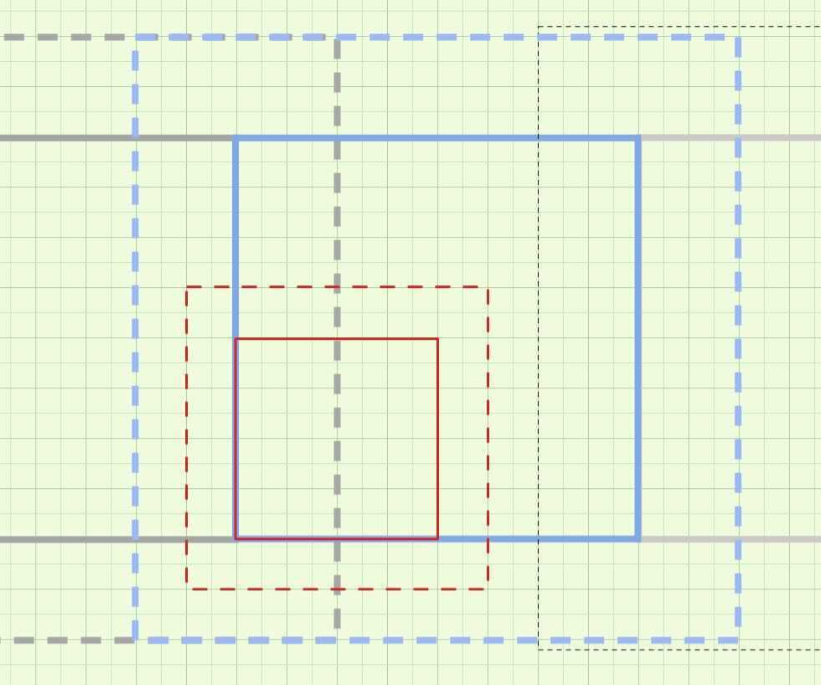
\includegraphics[width=0.5\textwidth]{guardzones.png}
    \caption{Illustration of guard zones related to overlapping patches at two levels of refinement.  The full drawn red square marks the zone of authority of the higher level patch, and the dashed red square marks the extent including the guard zones, which are assumed to be two cells on each side. Correspondingly, the blue full drawn and dashed squares show the parent patch at the lower level, from which the red patch was spawned.}
    \label{fig:guardzones}
\end{figure}

An accelerated form of the list of actions is
\begin{enumerate}
    \item A thread updating a level $L+1$ task creates a level $L+2$ child task
    \item Because it was formed with complete guard zone data, the thread can update the level $L+2$ task immediately.
    \item The thread then creates a new nbor list for the $L+2$ task.   
    \item Next the thread calls \Code{check\_support} on the new task, to discover if support is missing, and if so, which level $L$ task it is that needs to be refined, in order to create support.
    \item The thread then sets array entries in \Code{patch\%frefine(:,:,:)} for the level $L$ task.
    \item If that nbor list has a level $L$ nbor in a different MPI process, the level $L+2$ task is a virtual task and gets copied over to the other MPI process.
    \item In that other process, one of the actions of a virtual task is to also generate an nbor list, and run a \Code{check\_support}, which discovers that the task is unsupported (also seen from the no-support bit), and hence sets the request bits in the level $L$ task
    \item If instead that level $L$ task is local, the thread adds entries to its '\%request' array.
    \item The level $L$ nbor refines, creates the missing level $L+1$ task, updates it, adds an nbor list to it, and sends a copy as a virtual task back to the 1st MPI process, which owns the level $L+2$ task.
    \item The new level $L+2$ task updates for the 2nd time.
\end{enumerate}

The list of actions that a thread should go through is
\begin{enumerate}
    \item Refine the level $L+1$ patch being updated, if required
    \item Update the child patch, which is born with filled guard zones
    \item Add an nbor list to it
    \item Run \Code{check\_support} on the task, and add requests to the appropriate level $L$ nbor(s).
\end{enumerate}

In this scheme, there are two types of check for support: 1) checking from the $L+2$ level if a patch has support, and if not to notify the level $L$ level patch that needs to be refined, and 2) checking from the level $L+1$ patch if support requirements prevent it from being derefined.

Checking if a level $L+1$ patch may be derefined without any level $L+2$ patch loosing support requires only checking if it has any level $L+2$ nbors that depend on it (\Code{nbor\%needs\_me==.true.}), because if that is the case, that nbor would instead have a level $L$ patch in its place. 
%%%%%%%%%%%%%%%%%%%%%%%%%%
\subsection{Task addition}
When tasks are added due to refinement there is no risk that the same task is attempted to be added by two different threads at the same time, since only one thread at-a-time can check for refinement of the parent task.   But when threads are added because of a need to add support, two threads could indeed attempt to add the same task, for different reasons, at the same time.   To prevent this, the addition of tasks to the task list should use a protocol that relies on the OpenMP lock associated with the hash table.  When a thread has decided that it wants to create and add a new task at a certain position and level, it should
\begin{enumerate}
    \item attempt to make a reservation in the hash table for the new task key, under lock
    \item if the reservation succeeds, prepare the task and add it to the task list, replacing the hash table entry for the task key
    \item in the mean time other threads can acquire the lock briefly, check existence and release or add their proposed task, depending on existence
\end{enumerate}
In order to keep the lock for as short a time as possible, the lock can be released as soon as a valid task ID and a valid \verb|task%link| have been created (along with other properties that will exist at the time such as position and refinement level).  Pseuo-code:
{\small\codecolor\begin{verbatim}
call refine%lock%set ()
if (hash_table%reserve(key)) then
  ...
  call task%pre_init ()
  call refine%update(key,link)
  call hash_table%lock%unset ()
  ...
  call task%init()
  ...
else
  call refine%lock%unset ()
  ... abandon ...
end if
\end{verbatim}}
A problem is that if the normal \verb|hask_list%get_link(key,link)| does not return \verb|null()|, other procedures may attempt to used the link, before it points to a valid task link.  On the other hand, the protocol in the meantime only needs the \verb|hash_table%reserve(key)| functionality, which may be constructed to return true when the key entry exists, but is not pointing to a valid task link.   Specifically, the hash table entry for the preliminary key could be an integer,or (better) could be a pointer to an easily recognizable skeleton task link

%%%%%%%%%%%%%%%%%%%%%%%%
\subsection{Task removal}
Task that are removed by derefinement cannot be immediately removed, since parallel task updates where the task is included in the nbor lists may already be committed to the queue.  The \verb|list%remove_and_reset()| procedure handles this, in collaboration with the \verb|link%garbage_collect()| and \verb|link%garbage_remove()| procedures.  Tasks that should be removed are tagged with \verb|bits%remove|, and are immediately removed from the task list and task hash list, which prevents them from being included in future nbor lists created by \initnbors{}.  Tagged tasks are still included in halo operations (but see below), but are not considered in \checkready{} or \checknbors.  Since \initnbors{} is called after AMR task updates the tagged tasks will at most participate in updates that were already queued or active when the remove tag was added, except the fact that they are ignored in \checkready{} may have the result that additional tasks that have them in their nbor lists schedule them.  This is a potential problem, since time constraints are then not considered, which may result in excessive time extrapolation (but see below).

\def\nneeded{\Code{task\_\%n\_needed}}
\def\needsme{\Code{nbor\_t\%needs\_me}}
Tasks are removed from the garbage list and deleted when the reference count \nneeded\ reaches zero.  The reference count is incremented by one whenever nbors are added to the nbor list, and are decremented by one when the task is removed from an nbor list.

Assume that task A need task B, but task B does not need task A.  Then task A is still in the nbor list of task B, and needs to exist as long as it on the list.  The reference counts of both A and B should be one, if no other tasks are involved.  If task A at some point is marked for removal in AMR, it needs to be kept as longs as it is in the nbor list of B, even if it is not needed by B, because when task B updates, it needs to still refer to task A, particularly because task B needs to discover that task A is marked for removal, and hence should not be included in a renewed nbor list.

This simple example show that the reference count for a task musts be incremented whenever the task is added to an nbor list, for whatever reason, and it must be decremented whenever the task is removed from an nbor list.

Reference counts to a task can, if counted correctly, only reach zero when its task list has been removed and a new one has not been added.  The nbor list is removed when the task is removed from the task list and has the \Code{bits\%remove} bit set in its status word.  The task could then still be included in the nbor lists of other tasks, and must remain in existence as long as there are \Code{nbor\%task} pointers that point to it.  Tasks with the remove bit set could still be used in guard zone operations, even though they have the remove bit set.  Tasks that have it in their nbor lists with the \Code{nbor\%needed} flag set may need it in guard zone loading operations.

\verb|task%n_needed| should not hit zero until the task no longer appears in any nbor list.  Task \verb|n_needed| can only decrease when a task has first been marked for removal (does not change \verb|n_needed|), which prevents it from being added in the next \verb|add_nbor()| call, so the \verb|n_needed| is not incremented then, and is subsequently decremented to zero, when the last nbor list the task is present on is removed by \verb|link_t%remove_nbor_list()|, which has write-lock protection.  If all use of nbor lists is protected by at least a read lock, the count can thus never reach zero during such a use.

%%%%%%%%%%%%%%%%%%%%%%%%%%%%%%%%%%%%%%%%%%%%
\subsubsection{Ignoring tasks under removal}
Tasks that are removed have their nbor lists removed immediately after being marked for removal, and hence the \verb|task%n_needed| is decremented for every task in that nbor list that was marked \verb|%needed|.  But the main mechanism that decrements the \verb|task%n_needed| count is that after a task has had its \verb|%remove| bit set, it will be removed from the nbor lists of all tasks that have it in their nbor lists.  Therefore, a task marked for removal should be up for final deletion as soon as all the tasks in its nbor list have updated once.

Since the nbor list is removed immediately, the \verb|bits%remove| should in principle be used to prevent any attempt to use the nbor list, but on the other hand such use is typically a loop over the list, and if skipping the loop is sufficient response there is no need to check the remove-bit.  This is the case inside \checkready{}, and \checknbors{}, while in \verb|halo%update()| a test is needed at the top, to trigger an immediate return.

%%%%%%%%%%%%%%%%%%%%%%%%%%%%%%%%%%%%%%%%%%%%%%%%%%%%%%%%%%%%
\subsubsection{Task deletion based on \Cod{\%n\_needed} counts}
With this method (handled by data type \Code{garbage\_t} in \File{link\_mod.f90}, the access count of tasks (\verb|task%n_needed|) is used to decide when to delete tasks (after deallocating their various resources).

The principles at work is that every task that is added to an nbor list with the attribute \verb|%needed| set has the count incremented, and every task removed from an nbor list has the count decremented.   Since nbor lists are updated by first building a new list (no lock needed), and then swapping the pointer and removing the previous nbor list under lock, a task that survives has its access count unchanged, while a task that is removed results in a decrement of the access count.

The nbor list of the removed task does not need to be removed, and in fact it may be used to check and reconcile the \verb|%n_needed| counts of itself and its nbors.  At the point in time when a task A is marked for removal, and is removed from the task list, one should use the nbor list to make sure the count is correct.  To do this, one runs through the task A nbor list, counting the number of tasks that needs it (incrementing a counter by one if \verb|nbor%needs_me| is true).  To ensure that the count is correct, the counting should be done before setting the remove bit, to avoid that the nbor tasks start removing task A from their nbor lists during the count.

If the task relations are ensured to be symmetric at all times (task A marked as needed by task B means task B is marked "needs me" by task A), the count should match \verb|taskA%n_needed|.  After the remove bit is set, other threads may start removing the task from other nbor lists, while atomically decrementing the task A counter.

Every time the garbage list is reviewed for potential task deletion, one can do an authoritative update of the reference count, but looping over nbors nbors, counting how many times task A turns up as needed in the nbor lists of nbors marked with \verb|%needs_me|.
{\small\codecolor\begin{verbatim}
    for nbor in nbors:
        if nbor.needs_me:
            n0 += 1
            for nbornbor in nbor.link.nbors:
                if nbornbor%needed:
                    if nbornbor%task%id == task%id:
                        n1 += 1
\end{verbatim}}

%%%%%%%%%%%%%%%%%%%%%%%%%%%%%%%%%%%%%%%%%%%%%%%%%%%%%%%%%%%%%%%%
\subsubsection{Task deletion based on \Code{\%needs\_me} counts}
Since a task can have a larger number of \verb|%needs_me| counts than \verb|%needed| counts, and since counting \verb|%needs_me| is done on the task itself, while \verb|%needed| is counted on the nbor lists of its nbors, it is simpler and more correct to base task deletion on \verb|%needs_me| counts.  This means the counting can in principle be done based on single task attributes; i.e.\ the counting could be done exactly where it is needed, namely in the \verb|link_t%garbage_remove()| procedure.

Using this alternative method requires, however, that tasks not only keep, but also \textit{update} their nbor lists after removal.   With this method, a task A with the \verb|%remove| bit set matures towards removal when tasks B that had it on their nbor lists remove it from their nbor lists, set the \verb|%init_nbors| bit on tasks in their nbor lists, and then only if the removed task A actually updates it nbor list.   This would thus require substantial changes to the action decision for task with the \verb|%remove| bit set.

%%%%%%%%%%%%%%%%%%%%%%%%%%%%%%%%%%%
\subsubsection{Code considerations}
Tasks to be removed should be immediately marked with \verb|task%set(bits%remove)|. The setting should be done under lock, and procedures that test for the remove-bit should do so under the same (read-)lock (which must be held until the task is no longer referenced).  Tasks marked with the remove-bit   
\begin{itemize}
    \item should be skipped when \verb|%check_nbors()| walks an nbor list
    \item should immediately return in \verb|%check_ready()| (in case the remove-bit was not set under lock)
    \item should be skipped in \verb|%init_nbors()| (eg. to prevent seg faults if testing for overlap), so they are not included in new nbor lists, but they
    \item must \textit{not} be skipped in \verb|halo%update()| or any other context where the task is \verb|%needed|, since their removal from nbor lists may not yet have taken place, and they are thus actually needed
    \item tasks in the garbage bin must have tasks marked for removal removed from their nbor lists, which implies their nbor lists must be updated, even though they are in the garbage bin
\end{itemize}
One should be able to assume that a tasks nbor list, when including all \verb|%needs_me| entries, includes all tasks that could possibly have \verb|%needed| set for the task.   Therefore,
\begin{itemize}
    \item one can handle the last item above by walking the nbors nbor list, removing references to tasks marked for removal.   Tasks marked for removal are allowed to exist precisely because, and only if, they are needed by still active tasks; they should never need to exist in the nbor lists of tasks marked for removal.  Hence
    \item when a task is added to the garbage list, the procedure should walk through the garbage list and either remove the task from those nbor lists, or else (simpler) mark them \verb|%needs_me=.false.|, so the next time the task is checked for actual deletion, the count is correspondingly decreased.
\end{itemize}

%%%%%%%%%%%%%%%%%%%%%%%%
\subsection{Guard zones}
As illustrated by \Fig{guardzones}, computing the two layers of guard zones for the red patch requires three layers from the blue patch; its two guard zone layers, and one internal layer.

In general, obtaining guard zones from neighboring patches requires first time interpolation and then interpolation in three dimensions, and here information from two different patches are required at each cell.

The procedure may be simplified considerably by first filling in the guard zones from the neighboring patch at the lower level, e.g. from the patch (L) to the left of the blue (P = parent) patch.  This requires nothing more than a guard zone fill at the same level, which is an already existing operation involving only time interpolation.

Since actually updating the memory values of the parent patch would require intricate memory locking, since it would risk interfering with another threads work on the same parent patch.  Therefore, it is better to create a clone of the parent patch, and load it with the relevant guard zone and restricted values.  Note that the corresponding loop should be over the child neighbor list, not the (longer) parent neighbor list.  

The relevant part of the blue patch is then obtained by restricting the values from the red patch---this is also an operation that is required in other contexts, so it already exists.

One could achieve this as a normal halo operation, by defining a task link and attaching to it the child nbor list.  It requires in principle only
{\codecolor
\begin{verbatim}
    allocate (halo_t:: link)
    link%task => clone
    link%nbor => child%nbor
    call link%update
    deallocate (link)
\end{verbatim}}

The final operation then consists of prolonging the blue patch values into the relevant part of the red patch guard zones.  In summary, here is pseudo-code for the operations:
{\codecolor
\begin{verbatim}
   subroutine %update (self)
     class(halo_t):: self
     ...
     if (self%needs_clone()) then
       call self%make_clone ()
       call self%clone%guard_zones_from (child%link%nbor)
       call self%guard_zones_from (clone)
     else
       call self%guard_zones (self%nbors)
     end if
\end{verbatim}}
Here we need one (normal) operation, which takes a patch (or clone) as one argument, and a neighbor list as another argument:
{\codecolor
\begin{verbatim}
   subroutine guard_zones_from (self, patch, nbors)
     class(halo_t):: self
     class(patch_t):: patch
     class(guard_t):: nbors
     ...
     nbor => nbors
     do while (associated(nbor))
       call nbor%task%update (patch)
       nbor => nbor%next
     end do
     ...
\end{verbatim}}
and we can use the very same procedure for the final guard zone fill of the child, by allocating a guard data type which has the clone as the task to pick up values from.
{\codecolor
\begin{verbatim}
     class(guard_t):: nbor
     ...
     nbor%source => clone
     nbor%target => child
     call nbor%update()
     ...
\end{verbatim}}

%%%%%%%%%%%%%%%%%%%%%%%%%%%%
\subsubsection{Index ranges}
To compute the index ranges relevant in the source and target patches one first finds the intersection of the internal part of the source patch with the guard zone part of the target patch.  In the case with the parent (P) and child (C) patch, the intersection is the red dashed square.

The corners of that square is converted to target index space by computing floating point index values and rounding up, while to compute to source patch index values one converts the corner coordinates to floating source index values, rounding down to integers.

%%%%%%%%%%%%%%%%%%%%%%%%%%%%%%%%%%%%%%%
\subsubsection{Prolong contexts}
Prolonging (interpolating to a larger resolution) is used in three contexts in DISPATCH:
\begin{enumerate}
    \item \textit{When creating new tasks in AMR:}  In this case the source patch is the parent patch, and all source cells can be used, since the parent task is by definition ready to be updated when the \verb|refine%check()| call is made.  In this case the target time is the same as the source time.
    \item \textit{When prolonging the gravitational potential:} This is also a case where the source patch is the parent patch, and where all source patch cells are valid, since they were interpolated to, at the correct time, and those guard zone values are not overwritten.
    \item \textit{When prolonging the `coarse clone':} The temporary clone of the parent patch is used to fill all guard zone values of the target patch in the \verb|halo%make_coarse()| call, so in this context the prolongation occures together with \verb|all_tgt| set to true.
\end{enumerate}
In context 2, only the gravitational potential is involved, so one can make use of the fact that it's a single unstaggered variable, all source cells are valid, and all target cells are to be used.  The \verb|interp%in_xyzt_stg()| procedure takes advantage of this special case.  It also used to prolong the gravitational potential, if it is present, in contexts 1 and 3.

In contexts 1 and 3 all \verb|%nv| variable indices are used, so the procedure needs to be able to cope with staggered variables.  The case is handled by the  \verb|guards%prolong()| procedure, which used to calls \verb|conserve%prolong| for the HD variables (to conserve mass, momentum, and thermal energy per unit volume) as well as possible), and calls \verb|guards%differ()| for the magnetic field (staggered) components.

The \verb|interp%in_xyzt_stg()| procedure is capable of dealing with staggered variables, and has been shown to agree exactly (bitwise) with the \verb|guard%differ(...,linear=.true.)| call in the case where the source patch contains the target patch, which as discussed above is the case of interest.

If one uses \verb|guards%differ| for HD variables, without the \verb|linear=.true.| option, it uses \verb|interp%in_t| to do time interpolation (in the log for \verb|%unsigned| variables, and variables transformed to per-unit-mass for \verb|%pervolume| variables), and the procedures \verb|%in_{x,y,z}| to do interpolation in space.  Variables that have been transformed to per-unit-mass or log values are transformed back in \verb|guards%unwind()|.

To summarize:  All three contexts concern cases where \verb|all_src| is true, which simplifies the necessary procedures a lot.  In context 1, one can also cut the cost in half, by utilizing that no time interpolation is needed.  Context concerns a single variable, while context 1 and 3 concerns all five HD variables.  They are in unstaggered in Ramses-like solvers, but staggered in Stagger/Bifrost-like solvers.

We can choose to call, generically, \verb|guards%prolong| explicitly, and let that procedure decide which method to use.  The procedure that is chosen by \verb|guards%prolong()| must respect staggering, and must respect the \verb|all_tgt| flag, which decides whether to fill also the ROA with values (context 1 and 2), or only fill the guard zones (context 3).

We can decide to use \verb|interp%parent_to_child| in contexts 1 and 2, and \verb|interp%in_xyzt()| in context 3.

%%%%%%%%%%%%%%%%%%%%%%%%%%%%%%%%%%%%%%%
\subsubsection{Prolong using all cells}
Interpolation to a patch at a higher level (not necessarily corresponding to a factor of 2 refinement) is allowed to use all cells in the source (parent) patch always, since such interpolations occur in only two situations:
\begin{enumerate}
    \item Since refinement is considered immediately before a task update, the parent patch already has guard zones filled in and all of its cells may thus be used when creating the child patch.
    \item When loading guard zones of a child patch, at any level, and where some of the neighbors of the child patch are not yet refined, the first step in the process is to create a clone of the parent patch and fill its relevant guard zones from the neighbors of the child patch, and hence again all cells that are relevant are also valid. 
\end{enumerate}
Note that in the 1st case the interior target cells are included, while in the 2nd case they are not. Therefore, there is an optional \Code{all\_tgt} argument, which controls if the interior is included or not.

%%%%%%%%%%%%%%%%%%%%%%%%%%%%%%%%%%%%%%%%%%%%%%%%%%%%%%%%%%%%%%%%%%
\subsubsection{Prolong in the context of reading RAMSES snapshots}
After reading in all RAMSES octs and using the values to partially fill the larger DISPATCH patches, there are many unfilled cells in those patches that need to be filled by prolonging from lower level patches.  The root grid level is the highest level that is guaranteed to be filled, and hence one can start a recursive process from this level, filling in (only) the cells at the next level that are not already filled.  Continuing the process to the highest level, one ends up with filled cells at all level
This process differs marginally from the process of filling new AMR patches with values for the first time, in that one must prevent the already existing values from being overwritten, using the \Code{\%filled} attribute that is also used in other contexts.

%%%%%%%%%%%%%%%%%%%%%%%%%%%%%%%%%%%%%%%%%%%%
\subsubsection{Handling pointer allocations}
To avoid that the child task inherits pointers pointing to the same object as in the parent task, it is important that all allocations that are made when calling \Code{experiment\_\%init} do \textbf{\textit{not}} check if the pointer is already associated.  The code should be such that the allocation takes place without testing, and any deallocation should be performed  programmatically and intentionally.   If this is adhered to it is not necessary to nullify a lot of pointers when a child task has been created.  

The code structure should of course be such that permanent allocations are only done once per task.  Memory that is only used temporarily should be explicitly deallocated when a task has finished updating, and should be allocated at the start of each task update, without testing if the pointer is associated.   A test is only allowed (while still being redundant) if the pointer is explicitly nullified upon deallocation.  Note that only the original pointer is actually nullified automatically when deallocating, so it is a good idea to explicitly nullify pointers that are to be tested.  But since this just adds redundant work it is simpler to not test, and not nullify.

%%%%%%%%%%%%%%%%%%%%%%%
\subsubsection{Example}
If the patches are $8\times 8\times 8$, with 2 guard zones, the full array has 12 elements in each direction, which we number from 1 to 12.

The steps outlined above are thus, with specific index ranges:
\begin{itemize}
    \item perform a same-level guard-zone load from path L to patch P, covering the x-index range 1-2 in P, corresponding to 9-10 in L, and covering at least the range 3-8 in y-index (which are the same in L and P).  Correspondingly, the range between corners (3,1) and (8,2) from the patch below (B), and the range (1,1)-(2,2) from patch (LB) in the lower left corner.
    
    Together, these guard zones and restrictions cover the entire range needed, which extends from (1,1) to (8,8) in P index space.
    
    \item After performing both the guard one loading and the restriction from the child patch (C) there is enough support to evaluate all cells in the range spanned from (1,1) to (12,12), while skipping the interior square (3,3)-(10,10).
    
    In 3-D, with $16^3$ patches, the ratio of all points to internal points is $(20/16)^3 = 8000/4096 \approx 2$, and hence it is probably more efficient to compute all values in a vectorized loop, marking out the interior with a \Code{merge(guardzone, internal, outside)}

    \item The x-index ranges relevant for the prolong operations are 1-3 in the source and 1-2 in the target on the left hand side, and 6-8 in the source giving 11-12 in the target, while in the y-direction index 1-8 in the source gives the range 1-12 in the target.
    
    The procedure starts with an $12\times 12\times 12$ array, which gives rise to a $12\times 12\times 20$ array by z-interpolation, and then y-interpolation gives a $12\times 20\times 20$ array, while finally x-interpolation gives the final $20\times 20\times 20$ array.  The number of cell interpolations is thus $12\times 12\times 20 + 12\times 20\times 20 + 20\times 20\times 20$, each involving two source points.
    
    Especially for larger, more realistic size patches, the gain is considerable, compared to $20\times 20\times 20$ operations, each involving 8 source points.
\end{itemize}

%%%%%%%%%%%%%%%%%%%%%%%%%%%%%%%%%%%%%%%%%%%%%%%
\subsection{Neighbor lists and synchronization}
The nbor list of a task is updated once per task update, to ensure that all tasks that are needed to provide guard zone information are included in the list, with the correct flags and statuses set.

The first time a task is introduced it may lack support, and if so it is marked with \Code{bits\%no\_support}, and is ignored until this status has changed, except for checking if the status has changed.  This is done by nbor tasks, when they update.  There is one particular nbor task that is the only one that needs to bother, namely the one that needs to make a refinement to add the lacking support.

An efficient method to handle this without constantly checking for support is to let the new task, which discovers that it lacks support, briefly acquire a task lock on the guilty nbor and set a status bit that triggers a refinement on support, the next time that task checks refinement.

The only other context in which the need for support must be checked is when a task is a candidate for removal; then it must be checked if it can be removed, without any of its nbors loosing support.   By putting that potential check last in the sequence, and skipping it if it is already clear it won't be removed, one can minimize the number of tests.

With the method indicated above, there is no need to ever include L+2 or L-2 tasks in the nbor lists.  A need for support can only arise when either a new level L+1 child task is created, in which case that task can figure out which level L-1 task that needs to know, and set the required bit on it.  That task can then figure out for itself which part of it that needs to be refined.  Apart from that, tasks need to check that support will not be list when they derefine.

Given that the parent level L task has all its level L-1 nbors in its nbor list, the parent level L task is indeed the one that is in the best position to find and signal the relevant level L-1 task that it needs to refine to provide support.

\begin{enumerate}
    \item Does this task need to be refined, in order to provide support.
    \item If "yes", then refine it, and do not add the L+2 task
    \item If "no", just ignore the L+2 task; do not add it to the nbor list
\end{enumerate}

The task nbor list must be updated after the task update, in order for the next round of check\_nbors() to include its nbors, and so the decision to add a task to the queue is always consistent with the actual status (uses the same nbor list) at the time when it gets attention and is to have its guard zones updated.

Hence the sequence of calls that a task link goes through must be 
{\codecolor
\begin{verbatim}
    call link%update                        ! loads guard zone values
    call refine%check_current (link)        ! check for refinement
    if (.not. derefined) then               ! if the task still exists
        call link%task%update               ! update the task
        call task_list%init_nbors (link)    ! update the nbor list
        call task_list%check_nbors (link)   ! check if any nbors are ready to update
        call task_list%check_ready (link)   ! check if the task itself is ready to update again
    end if
\end{verbatim}}
An nbor that is unrelated, except for being a new added nbor to the new task, may updated one more time before it detects the new nbor, via the {\initnbors} call.  This is OK, since the nbor was already OK with the parent L-1 task of the new level L nbor.

%%%%%%%%%%%%%%%%%%%%%%%%%%%%%%%%%%%%
\subsubsection{Temporary task lists}
It is possible (but perhaps a bit confusing) to add tasks to a temporary task list, e.g. for the purpose of doing subsequent processing.  To do so, one allocates a task list, and adds the tasks to it, while specifically avoiding to modify \Code{task\%link}, which should point to the link in the normal task list.  The \Code{\%next} and \Code{\%prev} links in the temporary task list, on the other hand, connect together the tasks in the temporary task list. For this to work, without doing damage to the permanent task list, it is crucial that the temporary task list add and removal procedures do not tamper with the \Code{task\%link} pointers. This is achieved by setting the optional \Code{keep} argument.

A safer and more transparent method is to use a doubly-linked list (\Code{dll\_t}) temporary list, pointing to the \Code{link} pointers with the anonymous \Code{dll\%car} pointer.

%%%%%%%%%%%%%%%%%%%%%%%%%%%%%%%%%%%%%%%%%%%%%%%%%%%%%%%
\subsubsection{Neighbor-list behavior for moving tasks}
When tasks are moving the nbor list needs to be updated for every timestep, since new tasks may be rotating into support need.  We therefore need a cheap and fast method to generate task lists, while leaving as few as possible in the list.

Running through the nbor lists of nbors is an efficient method to visit all possible new or obsoleted nbors.   One can either save their task IDs in a hash table, or else use a sorted list, where the \Code{add} method skips entries that are already there---this is very cheap if a linear sort is anyway employed.

%%%%%%%%%%%%%%%%%%%%%%%%%%%%%%%%%%%%%%%%%%%%%%%%%%%%%
\subsubsection{Simple logics to ensure level support}
\begin{itemize}
    \item The parent task generates the child patch, fills it with prolong, and generates an nbor list for it

    \item The parent calls the \hassupport\ procedure, which sets the \nosupport\ bit, and notifies nbors that need to refine (this requires that the child nbor list has been generated)

    \item The parent task then adds the child task to the ready queue, and otherwise proceeds as other tasks

    \item Tasks that update generate new nbor lists, which include the new child task

    \item Tasks with the no-support bit are ignored in \checkready, and hence do not get added to the ready-queue.  They are also ignored as nbors in \checkready, so tasks can keep updating

    
    \item Tasks that find non-zero \Code{target\%request} values refine, creating the support needed
    
    \item When a \Code{check\_nbor()} encounters an nbor-task with the \nosupport\ bit they execute the \hassupport\ procedure on it, and this eventually leads to success, including the clearing of the \nosupport\ bit---possibly as early as before the parent task runs its \initnbors\ and  \checknbors, if other threads have made the refinements needed in the mean time.   
    
    \item Optionally, tasks may remember whether they did a refine because of a refine request, and only run the \hassupport\ procedure if that was the case
    
    \item When the child task updates the very first time the halo-update procedure detects istep=0, and does not need to do more; this holds for IC-generated tasks, as well as for child tasks that have already been prolonged
    
\end{itemize}
These actions require the following hooks in a few procedures:
\begin{itemize}
    \item The \Code{check\_nbors} procedure needs to know if refinement was done due to a support request, and 
    \item it needs to detect the \Code{no\_support} bit, and make a call to \Code{nbor\%link\%has\_support()}, 
    \item which needs to set and clear the \Code{no\_support} bit
\end{itemize}

%%%%%%%%%%%%%%%%%%%%%%%%%%%%%
\section{Support}
A task at level L must have its guard zones covered by tasks at level L-1, L, or L+1.  If that is not the case, the task is not ready to be updated, so checking this could / should, directly or indirectly, be part of \checkready.  Since the presence of support can only change when the tasks nbor list is updated, it is logical to place the check for support immediately after the nbor list generation.

NOTE:  Many of the sub-sections below are out-of-date and redundant.  The current code is the result of a significant simplification, resting on the fact that if support is created immediately and recursively, by the thread that discovers the missing support, the process is much simpler.

This, in turn, relies on the fact that all parent tasks, needed to create the respective support tasks, must already exist on the rank, as real or virtual tasks.  Therefore, the one thread that discovers the missing support can do it all, as part of the \verb|refine%check()| call that created the level L+1 task, which turned out to have a missing level L nbor.

In pseudo-code:
{\small\codecolor\begin{verbatim}
refine%selective_refine:
  make_child_patch():                   ! just create the task (with parent pointers)
    create_patch():
      allocate(patch,link)
      patch%pre_init()
      patch%init()
      if parent%time>0:
        guards%prolong(parent,patch)
      else:
        task_list%init_task(patch)
  dll_list%append(child%link)           ! add to list of new tasks
  task_list%add(child_link)             ! add to the task list (makes visible)
    hash_table_add()                    ! adds the task to the hash table
  create_support(child):                ! create support tasks (recursively)
    loop over 8 corners:
      if not patch exists:              ! requires presence in hash table
        create_patch()                  ! call inside call (recursive)
        dll_list%append(patch)          ! add to list of new tasks
        task_list%add(patch)            ! add to task list
          hash_table_add()              ! add to hash table
        create_support(patch)           ! recursive call
\end{verbatim}}
So, in general, one AMR call can lead to the creation of large number of new tasks, which are initially added to a dll list, and which are also in the process added to the task list and the hash table.

If several threads were working on this at the same time, more than one thread could try to create the same new support patch.  This is prevented by adding tasks to the hash table under lock, and checking in the hash table if a task already exists.

Other tasks, being updated while the support is being added, could discover the new tasks prematurely, when using the hash table to look for nbors, and since one does not wants to halt all task processing while creating support, one needs to mark the tasks in such a way that they are not included and used prematurely; until they are fully incorporated (by having had nbor lists added, etc), these tasks should be ignored in the \verb|%init_nbors()| procedures.

Once the creation of support tasks is complete, the dll list of new tasks is processed, leading to the incorporation of the new tasks in the normal task cycle.  This is done in the \verb|refine%post_process()| procedure.  Pseudo-code:
{\small\codecolor\begin{verbatim}
refine%post_process():
  for each task in dll-list:
    clear(bits%update_nbors)
    task%init_nbors()
    task%set_update_nbors()
  for each task in dll-list:
    clear(bits%ignore)
  for each task in dll-list:
    check_ready(task%link)
  for each task in dll-list:
    dll_list%remove(task)
\end{verbatim}}
In words:  First create nbor lists for all new tasks, then check if any of them are ready to update, and finally remove them from the dll list.

Some of the newly created tasks may be boundary tasks.  If they are, then upon their first task update a copy will be sent to rank nbors, where they then appear for the first time, as new virtual tasks.

%%%%%%%%%%%%%%%%%%%%%%%%%%%%%%%%%
\subsection{Checking for support}
The only occasion where support is an issue is when AMR tasks are created and removed, so there is no need for a general method to check support for all tasks.  In the \verb|rerfine%create_support|, one uses the fact that any patch at level L+1 is contained inside a `parent' patch at level L, which is the patch from which it was first created by AMR (or else a parent patch created by \Code{list\_t\%make\_nbors}).  The level L+1 patch must lie in one of the 8 corners of the parent patch, and there are 7 other level L places surrounding that corner.  Hence, to check if a task has support or not, one just needs to check whether all of the 8 level L places around that corner are occupied or not.

%%%%%%%%%%%%%%%%%%%%%%%%%%%%%%%%%%%%%%%%%%%
\subsection{Immediate support mechanism}
This is the method of choice to ensure that all patches end up with support, while being essentially ignored until this is the case.  To see how it works, consider a task (C) created at level L+1 by a task (P) at level L.  If one or more of its required 8 nbors at level L is missing, the task lacks support.   The missing task(s) at level L need to be created from a grandparent task (G) at level L-1.  The grandparent task is not necessarily the parent of task (P), but it is for sure one of the tasks in the neighbor list (P-N) of patch (P).

With factor two refinement (assumed for now), each new child patch lies at one of the eight corners of its parent patch.  That corner is surrounded by up to 8 patches, on all levels below the child patch level. The 8 patches can be owned by up to 8 different ranks.\footnote{Note that a high level patch has 8 nbors on all levels only if it lies in a corner of the root grid.  In most cases most support levels have fewer patches, often only one.}

The location of the 8 support tasks on each level can be found easily by using the hash keys, with which one also can check if a task already exists there, or if one needs to be created.  To create the tasks does not require direct access to the level (L-1) tasks, only the same kind of time slice access that is normally used when downloading guard zones---and in fact those very procedures can and should be used to load the initial data.

One can create the necessary (S) tasks without lock conflict with other tasks, then find their parent tasks, add them to the task list, create their nbor lists, and (only) then activate them (to prevent them from becoming road blocks their status should exclude them from consideration in \checkready). 

Since the same thread that started to update task (P) also "owns" the new (S) tasks, it can download data to them with normal \Code{link\%update()} calls (although to cause prolongation into interior points, calls should have \Code{all\_tgt=.true.}).

In pseudo-code, creating a new task in AMR and ensuring that it has support:
{\codecolor\small
\begin{verbatim}
  check refinement criteria
    create child task
    do i=-1,1,2
    do j=-1,1,2
    do k=-1,1,2
      position = task%hash_position (key)
      key = task%hash_key (size=parent%size, level=parent%level)
      !... create missing tasks needed for support
    end do
    end do
    end do
\end{verbatim}}
\begin{figure}
    \centering
    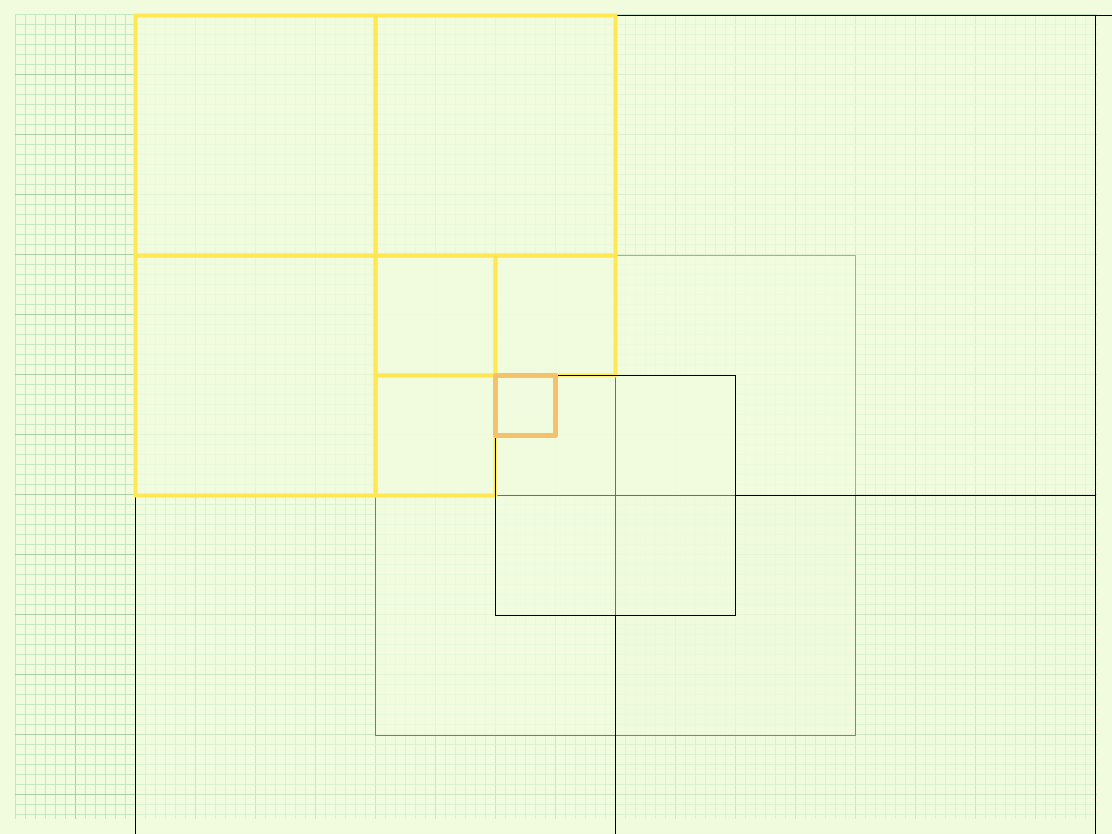
\includegraphics[width=0.7\textwidth]{RecursiveSupport.png}
    \caption{Figure illustrating the need for recursive generation of support.  The initial distribution of patches is symmetric; i.e., the upper left corner is identical to the other corners, with legal support for all patches, and with the arrangement continuing to larger scales as well.  Adding the small patch outlined with fat orange border results in the need to add three neighboring support patches, which in turn generate the need for three larger ones, \textit{etcetera}, over as many levels as there are missing patches in the upper left corner.}
    \label{fig:RecursiveSupport}
\end{figure}

\def\addnewlink{\Code{refine\_t\%add\_new()}}
\def\createpatch{\Code{refine\_t\%create\_patch()}}
\def\checksupport{\Code{list\_t\%check\_support()}}
\def\createsupport{\Code{refine\_t\%create\_support()}}
\def\createsupports{\Code{refine\_t\%create\_supports()}}
\def\suppportachieved{\Code{support\_acheived()}}

As illustrated by Fig.\ \ref{fig:RecursiveSupport}, the support generation mechanism needs to be recursive, with each new patch generating up to 7 new patches at the next lower level.  This is arranged by having a (recursive) \createsupports{}{} procedure, which creates the patch, adds an nbor list, classifies the patch, and then calls itself again.

The figure also illustrates, indirectly, that new patches will always be generated on top of already existing parent patches.

%%%%%%%%%%%%%%%%%%%%%%%%%%%%%%%%%%%%%%%%%%%%%%
\subsubsection{Potential dead-lock situations}
One of the risks of dead-lock comes from the fact that, even though nbor-lists are in principle symmetric, they are not updated simultaneously. This leaves potential possibilities for dead-lock.

One example is that AMR may create a new child task (A) that has another task (B) at the same level as an nbor, and that will therefore, sooner or later, rely on that nbor (B) to be the one that puts the task (A) back into the ready queue.  But if task (B) is derefined and removed before it has done that, task (A) would not be put back into the ready queue, unless task (B) on the one hand actually already has it on its nbor list, and on the other hand actually checks that nbor list for ready tasks, before it is removed.   Since tasks normally only update their nbor list after they update, but decide to be derefined before being updated, they must generate a new nbor list as the next-to-last thing, before checking the same nbor list as the last thing.

%%%%%%%%%%%%%%%%%%%%%%%%%%%%%%%%%%%%%%%%%
\subsubsection{Avoiding update dead-lock}
In general, there should be symmetry between the source and target, in the sense that when an nbor task B is marked as \Code{\%needed} in the nbor list of task A (which means task B is included when \checkready{} is run on task A), then task A must be marked \Code{\%needs\_me} in the nbor list of task B (which means running \checkready{} on task A is included when task B runs \checknbors{}), and vice versa.

When a new AMR task (N) is created, its nbor list is the first one that gets created, with a number of tasks marked as `needed'.  If the task is immediately subjected to \checkready{} and fails, it is depending on the tasks in its nbor list to eventually schedule it.  Each one of these task may be in an either idle, ready, or busy state at the time task (N) is created.  During the creation, their task status word is updated (atomically) with the init-nbors bit, so by the time they finalize their next update, they will generate new nbor lists that include task (N) with \Code{nbor\%needs\_me} set, and the subsequent \checkready{} on the task will eventually schedule it.

Since \Code{\%needs\_me} controls which tasks get checked for ready state, it is OK to have tasks marked as \Code{\%needs\_me}, even if the corresponding task does not have \Code{\%needed} set.  But since the \Code{\%needed} part is generally created before the corresponding \Code{\%needs\_me}, this is not of much significance.

The procedure to follow is basically
{\codecolor \begin{verbatim}
    def check_nbors(task):
        for nbor in task.nbors:
            if check_ready(nbor):
                if nbor.task.is_set(no_support):
                    nbor.task.clear (no_support)
                    nbor.needed = True
            queue_by_time(nbor.task)

    def check_ready(task):
        ok=True
        for nbor in nbors:
            if nbor.task_is_clear(no_support):
                if not nbor.task.is_ahead():
                    ok=False
\end{verbatim}}

Note that on the virtual task side, the task must also have the \Code{\%no\_support} bit set.  The bit will be cleared when one of the nbors to the real task discovers that it is ready to update.  Those nbors include the virtual nbors, which indeed also execute the \checknbors\ procedure.



%%%%%%%%%%%%%%%%%%%%%%%%
\section{Load balancing}
%%%%%%%%%%%%%%%%%%%%%%%%
There are two types of load balancing; initial and dynamic.  Initial load balancing is what is needed when changing the number of MPI ranks, and dynamic load balancing is what should be going on continuously, at least in cases with active adaptive mesh refinement (AMR).

%%%%%%%%%%%%%%%%%%%%%%%%%%%%%%%
\subsection{Naming conventions}
Tasks that are owned and updated by a given process are called \textit{real} tasks, while tasks owned by other processes that are neighbors to real tasks are called \textit{virtual} tasks.  Real tasks that have virtual neighbors are referred to as \textit{boundary} tasks, and tasks that are owned by other processes and are not virtual tasks are referred to as \textit{external} tasks.

Processes that own virtual tasks are called \textit{neighbor processes}, while other processes are called \textit{external processes} --- both of course relative to any given \textit{owner} process.

%%%%%%%%%%%%%%%%%%%%%%%%%%%%%%%%%%%
\subsection{Initial load balancing}
When restarting with a different number of parallel processes ("ranks" in MPI lingo) the distribution of processes over ranks can and should be redistributed, and it is in general not optimal to rely on the dynamic load balancing for this.   A job could for example need to be restarted with many more parallel processes, and if the previous rank-assignment was used initially, many processes would start out empty, and could become filled with rather unrelated tasks, "sold" to it by other processes during dynamic load balancing.

During restart with the \File{restart\_mod.f90} code it is easy to perform initial load balancing, because
\begin{itemize}
    \item the metadata of all processes that wrote a snapshot are initially read in, but no memory is allocated.  In the next step, the initial load balancing algorithm, which is the same in all processes, decides on a rank distribution, and all processes also compute the neighbor lists of all tasks.
    \item Each process then keeps both a) the (real) tasks that are assigned to it, and b) all (virtual) tasks that are on the nbor list of one of the real tasks, and then deletes all remaining tasks
\end{itemize}

%%%%%%%%%%%%%%%%%%%%%%%%%%%%%%%%%%%%%%%%%%
\subsubsection{Nearest neighbor algorithm}
In this algorithm, the load balancer assigns a position to each process, in a predictive way that results in the same position outcome in all processes.  Each process also computes the total cost of all processes, using the \Code{task\%cost} as a measure of the cost of each task, and the total cost is divided into equal shares for each process.  

The load balancer algorithm then finds the process that is nearest to each of the "process points", and adds it as the first process in the task list of the corresponding process.  It then assigns additional tasks to each process, by adding neighbors of the already assigned tasks, taking care to use a predictive method that results in the same choices in all processes.  The algorithm stops when either the assigned cost is reached, or else when there are no more nbors available to assign.  In the latter case there are other processes that still have nbors left to assign, after reaching the shared cost goal.  The process is then continued until there are no nbors left.

The resulting imbalance can be left to the dynamic load balancing to take care of, or one could add another step in the initial load balancing process, where task are reassigned from ranks with below-average load, from ranks that have above-average load.

%%%%%%%%%%%%%%%%%%%%%%%%%%%%%%%%%%%
\subsection{Dynamic load balancing}
A dynamic load balancing module is implemented, with the only remaining work to fine tune which parameters to use to control the swapping of tasks.  There are several candidate metrics, and it may be better to combine several of them than to rely on only one:
\begin{itemize}
    \item[a)] The actual update cost per task, which can be measured or computed.  This is a very stable metric, and the experience from unigrid runs with near-perfect load-balancing shows that obtaining cost balance may well be enough.
    \item[b)] The size (or cost) of the ready-queue, which reflects if an MPI process is oversubscribed or starved for work, is another obvious metric. This is a metric that can fluctuate wildly and rapidly, but one can use a running mean of the value, optionally with provisions to use a non-linear mapping that emphasizes periods of very short queue lengths.
    \item[c)] The fraction of time that the ready-queue is empty
    \item[d)] The total number of neighbors (virtual tasks), relative to the total number of tasks on a rank
    \item[e)] The number of neighbors of a process that are virtual tasks -- under circumstances where the number of tasks on a rank should be reduced, choosing tasks that have already have several neighbors on a different rank is advantageous, since it will tend to reduce the communication load.
\end{itemize}
A good compromise is to rely mainly on a), and use b) as a correction, which takes care of unforeseen cost effects.  After deciding to change the balance one can then let c) and --- in particular --- d) influence with which neighbor rank one should make a trade.

The decision is always taken by the owner rank, which after deciding to "sell" one of its boundary tasks changes the \Code{task\%rank} and status bits, and sends it to the new owner, which recognizes that the task has been swapped from a virtual task to a boundary task, and takes the necessary action (creating new nbor lists, etc).

As a secondary consequence, tasks on the receiving rank that were previously internal tasks may become boundary tasks, which implies that the tasks need to be sent as virtual tasks to their corresponding neighbor ranks.

%%%%%%%%%%%%%%%%%%%%%%%%%%%%%%%%%%%%%%%%%%%%%
\subsubsection{Communicating load conditions}
Messages are already sent between ranks at exactly the relevant moments in time, namely when boundary tasks have just been updated, so it is natural and convenient to let rank load measures `piggy back' on that communication, by adding measures of task-list cost and task-list queue cost to those packages.  To make this information immediately available to all tasks, the unpacking of it should go to two arrays indexed by rank.

%%%%%%%%%%%%%%%%%%%%%%%%%%%%%%%%%%%%%%
\subsubsection{Load-balance decisions}
Decisions whether to change rank ownership of a task must be taken by the thread that updates task, with the decision effectuated by changing the \Code{task\%rank} value, and setting the \Code{bits\%swap} status bit.

A decision to pass ownership to one of the ranks in the neighbor list is based on the combination of two criteria; 1) passing over load from a rank with higher load to a rank with lower load, and 2) improving, or at least not deteriorating, the communication load.

The instantaneous load on all ranks is available in \Code{mpi\%load(0:mpi\%size)}, where the choice of exactly what measure to copy to that array is a different topic.

The communication criterion is most simply evaluated by computing how many nbors a task has with the same rank as itself on the one hand, and the number of nbors it has with any other given rank, on the other hand. If a task has more nbors with a rank that agrees with a particular nbor candidate task, then changing ownership will reduce the communication needs, while if the number of nbors is the same, the communications needs will remain the same.  

To compute the effect of changing the rank of a task, compute the number of neighbors that are owned by rank A and how many are owned by rank B (ignoring nbors owned by other ranks).  All tasks owned by rank B need communication before a swap, while all nbors owned by rank A need communication after the swap.  So, if more nbors are owned by B, the task has a tighter affiliation with B, and the number of communications will be reduced by a swap.

%%%%%%%%%%%%%%%%%%%%%%%%%%%%%%%%
\subsection{Task status changes}
A task can change from internal to boundary for two different reasons: 1) because it is discovered that it has a virtual nbor, or 2) because an nbor task is aspiring to make a swap from boundary to virtual, and forces its internal nbors to boundary status.  In the 2nd case the transition could be cancelled by the 1st rule, unless the 1st change is a one-way only change.

One could impose that any task that has an nbor with a virtual nbor is also a boundary task.  This would however roughly double the number of boundary and virtual task, and thus also the MPI bandwidth.  A better approach is to disable automatic status determination (\Code{link\_t\%check\_status}), and rely instead on event-driven status change.  Tasks could then be changed from internal to boundary before a load-balancing swap, and tasks could be changed from boundary to internal due to the explicit removal of its last virtual nbor. 

%%%%%%%%%%%%%%%%%%%%%%%%%%%%%%%%%%%%%%%%%%%%%%%%%%%%%%%%%%%%%%%%
\subsection{Typical conditions in jobs with many cores per rank}

Typical updates times with AN-family solvers are 0.5--1 core-microseconds.  With typical patch sizes somewhere between 4k and 32k cells, this gives update times of order 2 to 30 milliseconds per task, or 30 to 500 tasks per seconds per core, or up to 3000 tasks per seconds for 64-core ranks.  With typically 10\% of the tasks being boundary tasks, several hundred boundary tasks are updated per second.  

With ideally of order 100 tasks per core, the number of tasks per rank is of the order up to 5000, which means that an update of all tasks takes from a fraction of a second to a couple of seconds, depending mainly on the number of cells per patch.  If the queue of tasks ready to update is of order 5-10 tasks per core, or of order 5--10\% of all tasks, the queue can in principle go to zero size in less than 0.1 second, and load-balancing should be able to change the load significantly---say by a few percent---on such time scales, so it should be able to add or remove hundreds of tasks per second.   Since load-balancing operates on a task-by-task basis, this means it should be able to make decisions for basically every boundary task update, so the cadence should not be larger than a few, and a cadence of one should be acceptable.

This basically excludes scanning the whole task list for every load-balance call, and hence measures of the load should either be based on easily available attributes, such as queue size, or else tasks should maintain a measure of the total task load as part of their normal task updates.  The \Code{task\%cost} attribute is maintained by each task, and especially when using AMR it is crucial to only consider actually swapping ranks on task with significant cost, while on the other hand avoiding the fragment clusters of tasks with affinity in space onto many different ranks. 

To avoid scanning task lists, one can let each task update a rank-wide running mean (an instance of the \Code{running\_mean\_t} data type), which can be done using atomic arithmetic, and hence avoids the need for locks.

Each boundary task should also maintain an attribute that measures its suitability for reducing surface area, and each virtual task should be exposing the same attribute to its nbors.  The attribute should basically be the number of nbors with a given different rank, relative to the number of nbors with the same rank.  If each task message contained that attribute for each virtual task nbor, relative to the boundary task itself, then one can decide that swapping is favorable if the number of virtual nbors will decrease as a result of the swap.

It is crucial to use a load measure that takes the actual cost of each task into account, since otherwise a random occurrence of a large number of cheap tasks could trigger useless swapping of them.  The rank load is therefore expressed as a function of the ratio of the total cost of the tasks in the ready queue, relative to (a running mean of) the total cost of all tasks.

Another crucial aspect is to swap ownership of a task \textit{before} it updates, rather than after it updates.  If it sent to the nbor rank after it updates, it will take on the average about 100 task updates times before it adds to the load of the nbor rank, while if it swapped before updating, and the handling of swapped tasks is capable of launching it immediately, the load appears right away.

This requires that the \Code{task\_mesg\_t\%unpack()} procedure is able to either queue the task for immediate execution, or actually takes the necessary steps.  These include filling the guard zones of the new task (which since it is up-to-date has valid nbors), updating the task, and triggering new  nbor lists or status updates among the nbors.  Calling \Code{task\_list\_t\%update()} would cover the necessary steps, except for the fact that virtual tasks do not have complete nbor lists; they only retain nbors that are active tasks, while the new boundary task also needs new virtual nbors.

The new virtual nbors will however not be created until the nbors of the now virtual task on the original rank update their task status, in connection with creating new nbor lists. The new boundary task on the other rank can only update after those tasks update and are sent---for the first time---to that other rank.   Sequence of events:

{\footnotesize\codecolor\begin{verbatim}
On rank A                                          On rank B
-------------------------------------------------  --------------------------------------------------
task 1 changes from boundary to virtual -> sent    task 1 is received, and is added to the task list
task 1 generates a new nbor list, removing some    task 1 generates a new nbor list, some missing
task 1 nbors update, get new nbor lists & status   nbors of task 1 update & get new nbor lists
some bors become boundary tasks -> are sent        virtual task received may allow task 1 to updates
\end{verbatim}}

%%%%%%%%%%%%%%%%%%%%%%%%%%%%%%%%%%%%%%%%%%%%%%%%
\section{Positions, distances, and task overlap}
%%%%%%%%%%%%%%%%%%%%%%%%%%%%%%%%%%%%%%%%%%%%%%%%
For several reasons most operations should be based on relative positions rather than absolute positions,  Examples:
\begin{itemize}
    \item Periodic systems, where the same task may appear on two sides
    \item General relativity experiments, where absolute positions do not make sense
\end{itemize}
All tasks have positions (\Code{task\%position}), but these are to be interpreted as distances relative to the origin of some local coordinate system.  Positions in planet related objects (e.g. planet atmospheres) are given relative to the planet center (or the center of gravity of the planet and moons).   Positions in the solar system are given relative to the center of gravity of the system, etc.

The complexity added when using periodic coordinate systems can and should be hidden by using periodic mapping of positions only when computing nbor distances, while relying entirely on distances when computing task overlap.

Information of relative positions is carried by \Code{link\%nbor\%distance}, which is the distance of the neighbor \Code{link\%nbor} from the task \Code{link\%task}.  The distance is computed using \Code{task\_t\%distance\_to (task)}, which \textit{should be the only procedure in the entire code that knows about and implements periodic wrapping}. This allows, for example, a task to refer to another task as two distinct neighbor tasks.  

Procedures that decide overlaps of tasks and their guard zones must rely on distances instead of positions.  Hence the procedure signature must be similar to
{\codecolor \begin{verbatim}
    LOGICAL FUNCTION overlaps (self, nbor)
      class(link_t):: self
      class(nbor_t):: nbor
      ...
\end{verbatim}}
rather than
{\codecolor \begin{verbatim}
    LOGICAL FUNCTION overlaps (self, task)
      class(task_t):: self, task
      ...
\end{verbatim}}

%%%%%%%%%%%%%%%%%%%%%%%%%%%%%%%%%%%%%%%%%%%%%%%%%
\subsection{Periodic boundary condition wrapping}
The use of periodic boundary conditions causes challenges when mapping distances between points inside tasks.  To handle these challenges systematically one can rely on a few basic principles:
\begin{itemize}
    \item After rescaling the periodic box to occupy the interval [0,box) in all dimensions, a point that might otherwise be outside the interval is ensured to be inside my taking \verb|point=modulo(point,box)|, followed by remapping back to the absolute position of the box (known as \verb|task_list%position|, or \verb|patch%origin+patch%box/2|)
    \item Patches smaller than half the box size can have only a single periodic wrapping inside the the box, while patches with half the box size or the full box size are wrapped back in more than one way, potentially causing confusion and incorrect mapping
    \item However, mapping single points is safe and unique, and while it typically results in less efficient code, this is normally not a concern, since such large patches are updated infrequently.
\end{itemize}
Hence code that has significant performance impact should have separate sections for those large patches, while most patches can rely on mappings of corners to determine unique index ranges in overlapping source and target patches.  The optimized sections can rely on mapping the position of source patches to a relative distance from the target patch, when doing interpolations or conservative prolongation or restriction.

The optimized code can be used when both target and source patch are smaller than half the box size, while the non-optimized code should be used when both target and source patches are half the box size or larger.  If (in prolongation) the target patch is smaller than half the box size, then the larger source patch still can have only a single, unique distance from the target patch.  The same is true for restriction from a source patch smaller than half the box size.  In general, a patch smaller than half the box size can only overlap with a neighbor patch in a single, unique way, so the optimized code versions should be OK in all such cases. Since this pertains to all prolongation and restriction cases, it is important for optimal performance.

%%%%%%%%%%%%%%%%%%%%%%%%%%%%%%%%%%%%%%%%%
\subsection{Staggered mesh consideration}
When the source and target meshes are staggered by half a cell, the mapping of indices between source and target is correspondingly modified.  The periodic mapping is not modified \textit{per se}, but the index bounds and index mappings in general become different for each staggered memory component.  Mapping index ranges separately for each component, while maintaining fixed iteration offfsets and increments should make it possible to maintain optimized code.

For unstaggered meshes the mappings for prolongation and restriction inside the ROA are always 1-to-2 or 2-to-1: one ROA point is mapped to 8 ROA points, or 8 ROA points are mapped to 1 ROA point.  But staggered meshes lead to (net shift) of half a cell, which on ROA boundaries can cause 1 ROA cell to be mapped to for example 4 ROA cells and 4 ROI cells.

In practice staggered variables always represent fluxes in the staggered direction, and conservation then has a different meaning;  Values in the perpendicular direction should still be averaged 4-to-1, while in the staggered direction every 2nd value should be discarded when restricting, while being interpolated (rather than duplicated) when prolonging.  Hence completely different implementation is needed for staggered variables in any case.

%%%%%%%%%%%%%%%%%%%%%
\subsection {Regions}
Regions are defined by the floating point lower (\Code{l}) and upper (\Code{u}) coordinates of their corners in 3-D space.
{\codecolor \begin{verbatim}
  type, public:: region_t
    real(8), dimension(3):: l=0d0, u=0d0
  contains
    procedure:: volume
    procedure:: union
    procedure:: overlaps
    procedure:: covers
  end type region_t
\end{verbatim}}
Two regions overlap if the volume of the union of their regions is non-zero.  A region covers another region completely if the volume of the union is the same as the volume of that other region.

Examples of regions:
\begin{itemize}
\item The internal region of a patch
\item The guard zone that covers one face of a patch
\item The guard zone that touches an edge of a patch
\item The guard zone that touches a corner of a patch
\item The union of the internal region of a source patch and a target guard zone
\end{itemize}
All tasks have two basic regions defined: \Code{task\%authority} is the region relative to \Code{task\%position} over which the task has authority, and \Code{task\%interest} is the region of interest, over which the task may need information from neighboring tasks.  For patches, the internal region is the region of authority, while that plus the guard zones make up the region of interest.

As an example of using regions, while relying entirely on neighbor distances, here is a code snippet from \Code{halo\_t\%has\_support}:
{\codecolor \begin{verbatim}
    ...
    nbor_authority%l = nbor%distance + nbor%task%authority%l
    nbor_authority%u = nbor%distance + nbor%task%authority%u
    region = self%task%interest%union (nbor_authority)
    nbor2 => self%nbor
    request_refine = .true.
    do while (associated(nbor2)) 
      if (nbor2%task%level == self%task%level-1) then
        nbor_authority%l = nbor2%distance + nbor%task%authority%l
        nbor_authority%u = nbor2%distance + nbor%task%authority%u
        if (nbor_authority%covers(region)) then
          request_refine = .false.
          ...
\end{verbatim}}
The \Code{self\%task\%interest} region has no position offset, and neighbor task authority regions are defined using \Code{nbor\%distance}, allowing simple logic to determine if a task has support at \Code{self\%task\%level-1} or not.

%%%%%%%%%%%%%%%%%%%%%%%%%%%%%%%%%%%%
\subsection{Slightly tilted regions}
Slightly tilted regions should be placed in such a way the target ROI corner that extends the least distance into the source ROA hits cell \Code{mesh\%li}, while the corner that extends the furthest into the source ROA hits a fraction of a cell less than one further in, so its index location is \Code{mesh\%li + p}, where \Code{p < 1}.  With this choice the index range used for interpolations is the same as if the two patches were exactly aligned, and the index ranges of target and source may be obtained from
{\codecolor\begin{verbatim}
  call target%overlap (lt ,ut, source, ls, us)
\end{verbatim}}
Internally, the call uses only the target and source regions, and the distance from the target to the source, expressed in the target coordinates.


%%%%%%%%%%%%%%%%%%%%%%%%%%%%%%%%%%%%%%%%%%%%%%
\subsection{Coordinate system transformations}
\def\src{\mathrm{source}}
\def\tgt{\mathrm{target}}
Coordinate system transformations are performed with the help of \textit{rotation matrices} ($\rot$) (in the code \Code{patch\_t\%erot(3,3)}) associated with each patch.  These matrices have the unit vectors of the local patch coordinate system expressed in global Eulerian coordinates as columns, and the unit vectors of the global coordinate system expressed in local coordinates as rows.  In cylindrical shell geometry, this means that a patch at azimuth $\phi$ has a rotation matrix
\begin{equation}
\rot = 
\begin{bmatrix}
\ \cos(\phi) & -\sin(\phi) & 0\ \\
\ \sin(\phi) & \ \ \,\cos(\phi) & 0\ \\
         0 &          0 & 1\ 
\end{bmatrix}
\end{equation}
In conventional mathematical notation the matrix elements $e_{ij}$ have columns over which index $i$ varies, and rows over which index $j$ varies.  Index $i$ thus enumerates different rows, while index $j$ enumerates different columns, and hence, perhaps somewhat confusingly, $i$ is `row index' and $j$ is `column index'.

In the volleyball geometry, the rotation matrices are defined in \Code{sphere\_point\_t\%unit\_vectors} as
{\codecolor\small\begin{verbatim}
  self%e(:,3) = normalize(p)                               ! unit vector up
  self%e(:,2) = self%north_proxy                           ! vector with north component
  self%e(:,1) = normalize(cross(self%e(:,2),self%e(:,3)))  ! unit vector east
  self%e(:,2) = normalize(cross(self%e(:,3),self%e(:,1)))  ! unit vector north
\end{verbatim}}
These vectors are indeed column vectors, and hold the local unit vectors, expressed in global coordinates.
    
In the cylindrical arrangement the rotation matrices are defined in \Code{cylinder\_t\%finalize\_tasks}, by
{\codecolor\small\begin{verbatim}
  task%erot(1,:) = [ cos(phi),-sin(phi), 0d0]
  task%erot(2,:) = [ sin(phi), cos(phi), 0d0]
  task%erot(3,:) = [      0d0,      0d0, 1d0]
\end{verbatim}}

Vectors in the local patch coordinate system can be transformed to vectors in the global coordinate system by noting that each component in the global coordinate system is the scalar product of the local vector with the global unit vectors in the local system, which encourages that local vectors are considered to be column vectors, while global vectors are considered to be row vectors.  The transformations may thus be written
\begin{equation}
    \begin{bmatrix}
    g_1 & g_2 & g_3 
    \end{bmatrix}
    = \rot \cdot
    \begin{bmatrix}
    l_1 \\
    l_2 \\
    l_3
    \end{bmatrix} \,,
\end{equation}
while the transformation from global to local coordinates correspondingly is
\begin{equation}
    \begin{bmatrix}
    l_1 \\
    l_2 \\
    l_3
    \end{bmatrix}
    = 
    \begin{bmatrix}
    g_1 & g_2 & g_3 
    \end{bmatrix} 
    \cdot \rot \ .
\end{equation}
Note that both Fortran and Python have a \Code{matmul(a,b)} operation, where either \Code{a} or \Code{b} (or both) may be a matrix.  In Fortran, the operations above thus correspond to 
{\codecolor\small\begin{verbatim}
    global = matmul(erot,local)
    local = matmul(global,erot)
\end{verbatim}}

If coordinates in the global and local coordinate systems share a common origin these transformations are complete, while of they are relative to the centers of the local patches, the distance between the patch centers need to be taken into account, by being added either before (if given in the local coordinate system) or after the matrix multiplication (if given in the local coordinate system).

%%%%%%%%%%%%%%%%%%%%%%%%%%%%%%%%%%%%%%%%%%%%%%%%%%%
\subsubsection{Relative coordinate transformations}
To transform from one local coordinate system to another, for example in the context of guard zone interpolations, one could transform from one local system to a global system and then from their to another local system.  It is more convenient, however, to make use of a \textit{relative transformation matrix}, which has the local unit vectors of the `source' patch, expressed in the `target' coordinate system as columns, and correspondingly has he local unit vectors of the `target' patch expressed in the `source' coordinate system as rows.  It is thus clear that \textit{the `source' coordinates take the role of the `local' coordinates above, while the `target' coordinates corresponds to the `global' coordinates above} (common to a number of different `sources' that contribute to the same `target'). Useful ``rules of thumb'' are thus that
\begin{itemize}
    \item \textbf{local} and \textbf{source} vectors are \textbf{column vectors}, while
    \item \textbf{global} and \textbf{target} vectors are \textbf{row vectors}.
\end{itemize}

The equations that correspond to the ones above are then
\begin{equation}
\rot = 
\begin{bmatrix}
\ \,\cos(\phi_\src-\phi_\tgt) & \sin(\phi_\src-\phi_\tgt) & 0\ \\
   -\sin(\phi_\src-\phi_\tgt) & \cos(\phi_\src-\phi_\tgt) & 0\ \\
             0 &          0 & 1\ 
\end{bmatrix} \,,
\end{equation}
\begin{equation}
    \begin{bmatrix}
    t_1 & t_2 & t_3 
    \end{bmatrix}
    = \rot \cdot
    \begin{bmatrix}
    s_1 \\
    s_2 \\
    s_3
    \end{bmatrix} \,,
\end{equation}
and
\begin{equation}
    \begin{bmatrix}
    s_1 \\
    s_2 \\
    s_3
    \end{bmatrix}
    = 
    \begin{bmatrix}
    t_1 & t_2 & t_3 
    \end{bmatrix} 
    \cdot \rot \ .
\end{equation}
Since the transformation from source to target can also be achieved by first translating the source coordinates to global coordinates and then go from there to target coordinates, it follows that the relative transformation can be obtained as the product of the transposed target rotation matrix and the source rotation matrix:
\begin{equation}
    \begin{bmatrix}
    g_1 & g_2 & g_3 
    \end{bmatrix}
    = \rot_\src \cdot
    \begin{bmatrix}
    s_1 \\
    s_2 \\
    s_3
    \end{bmatrix} \,,
\end{equation}
\begin{equation}
    \begin{bmatrix}
    t_1 \\
    t_2 \\
    t_3
    \end{bmatrix}
    = \rot_\tgt^T
    \cdot
    \begin{bmatrix}
    g_1 & g_2 & g_3 
    \end{bmatrix} \,,
\end{equation}
Hence
\begin{equation}
    \begin{bmatrix}
    t_1 \\
    t_2 \\
    t_3
    \end{bmatrix}
    = \rot_\tgt^T \cdot \rot_\src
    \cdot
    \begin{bmatrix}
    s_1 \\
    s_2 \\
    s_3
    \end{bmatrix} \,,
\end{equation}
and
\begin{equation}
    \rot_{\src\rightarrow\tgt} = \rot_\tgt^T \cdot \rot_\src
\end{equation}
The \Code{matmul} standard Fortran procedure has the same convection as the corresponding procedure in Python; multiplication uses the index in a matrix that is ``closest'' to the vector, so when multiplying with the matrix on the left, the index that runs over the vector components also runs over the 2nd index of the rotation matrix, and thus follows common mathematical conventions.

As per the equations above, source vectors are `column vector', which combine with rows in the matrix (2nd index varying), while target vectors are `row vectors', which combine with columns in the matrix (1st index varying).

The code procedure \Code{task\_t\%get\_position} is consistent with the discussion above \textit{if} the call sequence below is used:
{\codecolor\small\begin{verbatim}
    call target%get_position (source, p=position, e=rotation)
\end{verbatim}}
Transformation of a point \Code{p} in target coordinates to the source coordinate system is done by using the position of the source center in target coordinates, and the rotation matrix:
{\codecolor\small\begin{verbatim}
    call target%get_position (source, p=p, e=e)
    src_p = matmul(e,tgt_p-p)
\end{verbatim}}
while the reverse transformation is
{\codecolor\small\begin{verbatim}
    call target%get_position (source, p=p, e=e)
    tgt_p = matmul(src_p,e) + p
\end{verbatim}}
In the 1st case one must adjusts for the location of the source while still in target coordinates, before the rotation to source coordinates.
In the 2nd case one must first rotate to target coordinates, before one can add the distance, which is known in target coordinates.

%%%%%%%%%%%%%%%%%%%%%%
\section{Input/Output}
%%%%%%%%%%%%%%%%%%%%%%
The ideal I/O method should
\begin{enumerate}
    \item not require synchronization between different ranks
    \item ideally write binary data from all ranks to one file per snapshot 
    \item not rely on knowing exactly how many tasks that will eventually be written for each snapshot
    \item use only a single thread on each rank to do the actual writing to disk -- thus avoiding slowing down the simulation during snapshot writing
    \item use a linked list of buffers to accept input from a large number of threads, which need to spend only minimal time adding it's buffer to the list
    \item allow output files corresponding to more than one snapshot to be open simultaneously
    \item allow any type of task output or input
\end{enumerate}

%%%%%%%%%%%%%%%%%%%%%%%%%%%%%%%%%%%%%%%%%%%%
\subsection{Attribute names and conventions}
The \Code{task\_t} data type contains these I/O related attributes:
{\small\codecolor\begin{verbatim}
    integer:: iout       ! the I/O sequence number, incremented by 1 for each new snapshot
    real(8):: out_time   ! cadence; the time difference between snapshots
    real(8):: out_next   ! the next output time for this task
    real(8):: start_time ! the first I/O time
    real(8):: end_time   ! the last I/O time
\end{verbatim}}
When a job restarts, possibly with a new I/O cadence, the \Code{task\%iout} is set to the same value for all tasks (typically \Code{io\%iout} or whatever is used by a task-specific restart module), and \Code{task\%out\_next} is set to the next multiple of \Code{out\_time}.

%%%%%%%%%%%%%%%%%%%%%%%%%%%%%%%%%%%%%%%%%%
\subsection{Snapshot output and data type}
Writing snapshot output in a context with task-local timesteps, and with task being created and removed by AMR on multiple threads creates some challenges; specifically related to 1) when a task should be written out, and 2) to decide when a snapshot is complete.

Each task type involved in an experiment that supports writing out snapshots needs to have a dedicated instance of the \verb|snapshots_t| data type, which is an extension of a double-linked list (DLL, \verb|class(dll_t)|).  Each member of that list is an instance of the \verb|snapshot_t| data type, with attributes that allow keeping track of for example how many tasks that have passed a given snapshot time.   The members of the list are indexed by snapshot number (\verb|snapshot%iout|), allowing a task that should do I/O at that snapshot number to find the associated file unit numbers for binary and metadata output, by searching in the list for a \verb|snapshot%iout| that matches its own \verb|task%iout|.  Tasks need to search only once for each snapshot time interval, since the result the search is saved as \verb|task%snaphost| (a DLL is simpler and has less organizational overhead than a hash table, and since the search is only done once speed is not an issue).  Once a task has reached the end of the interval, the output procedure detects this, does the I/O, increments the \verb|task%iout|, and finds (or creates) the next \verb|%snapshot| instance.

To decide when a snapshot is complete is challenging, especially when AMR is actively adding and removing tasks on multiple threads. However, a simple criterion can be used:  Since tasks are ordered by time in the ready queue, a snapshot is complete when the first task in the queue passes the corresponding \Code{out\_next} time, and the next task in the queue has already passed it.  Since (or if) all task output is rank-local, there is no need to synchronize this across ranks.

Different types of tasks (\eg\ patches, sink particles, and particle-in-cell tasks) may need to have separate output cadences, and hence different \Code{out\_time} values.

More generally, a snapshot of a particular task type is characterized by a file name, a data unit associated with the file name, possibly a record size and a record counter, etc..  Hence it is convenient to collect all attributes related to a snapshot into a \Code{snapshot\_t} data type, which could in principle also be a task, but is at least currently handled outside of the dispatcher normal task loop.

Multiple snapshot instances are handled by the \Code{snapshots\_t} data type, which is an extension of the doubly-linked-list (\Code{dll\_t}) data type.  It is thus able to hold an unlimited number of simultaneously open files.  The I/O module for a particular task type, \eg\ the \Code{sinks\_io\_mod.f90}, should contain an instance of \Code{snapshots\_t}, to hold the information required to handle several simultaneously open snapshot files for that particular data type.   For patches, the corresponding module is \Code{data\_io\_mod.f90}.

In order to allow for any number of different task type, each with their own cadence, the data structure should be changed to
{\codecolor\small\begin{verbatim}
data/run/00000/snapshot_00000.dat
                       snapshot_00000.nml
                       snapshot_00001.dat
                       snapshot_00001.nml
                       ...
data/run/00001/snapshot_00000.dat...
                       ...
...
data/run/pic/00000/snapshot_00000.dat
                   snapshot_00000.nml
                   ...
data/run/pic/00001/snapshot_00000.dat...
                   ...
...
data/run/sinks/00000/snapshot_00000.dat
                     snapshot_00000.nml
                     ...
data/run/sinks/00001/snapshot_00000.dat...
                     ...
...
\end{verbatim}}
The responsibility to create the \Code{data/run/pic/} and similar directories lies with the \Code{\%init()} procedure of the \Code{extras/} feature, assisted by a \Code{snapshot\_t} procedure.

%%%%%%%%%%%%%%%%%%%%%%%
\subsection{Stream I/O}
We need these data types and methods:
{\codecolor\begin{verbatim}
  snapshot_t:
    attributes: ntask, ...
    procedures:
  io_item_t:
    attributes: pos, buffer
  item_list:t
    attributes: head
    methods: append, remove
  stream_io_t
    methods: open, write, flush, close

stream_io_t:
  write
    call task%pack()
    call task%snapshot%list%append (task%mesg%buffer)
  flush
    item => snapshot%list%head
    do while (associated(item))
      next => item%next
      call item%write ()
      dealloate (item%buffer, item)
      item => next
    end do
snapshot_t:
packet_list_t:
  append
  remove
task_t:
  pack
  unpack
\end{verbatim}}

The  \verb|io/stream_io_mod.f90| module supports writing snapshots with I/O packet size varying between task.  The I/O packets should be completely analogous to, and interchangeable with, the MPI packets used to transmit copies of tasks between ranks.  Hence they must contain information not only about the packet size, but also about the task type, to allow both the snapshot reader and the message unpack procedure to identify the task type, and hence pick the correct task read/unpack procedure.  Both then reading I/O and receiving MPI, the steps thus are
{\codecolor\begin{verbatim}
    1. get the buffer
       *) when reading both offset and size should be in metadata
       *) when receiving MPI, the MPI_Improbe method gets the size and buffer
    2. find the task type and allocate an instance
       *) register task type; we need a task_factory_mod
       *) this cannot rely on knowing all possible task types
    3. call the task%unpack
\end{verbatim}}

%%%%%%%%%%%%%%%%%%%%%%%%%%%%%%%%
\subsection{High cadence output}
Some extras require separate output sequences, typically with higher cadences than the normal MHD snapshots.  Examples include dust particle and sink particle output.  These data types thus have their own \Code{\%out\_time} attributes, which specify the (instantaneous) output cadence.

It is desirable to allow the cadence to be changed during runs; e.g. at restarts, or through the interactive `flag'-mechanism.  This should happen without resulting in breaks of the snapshot number, so whenever the cadence changes, a calculation such as the one below needs to be used to compute the next output time:
{\codecolor \begin{verbatim}
    task%out_next = ceiling(task%time/task%out_time)*task%out_time
\end{verbatim}}
When that time arrives, the task needs to refer to increment the snapshot number it is writing to, with a code snippet similar to
{\codecolor \begin{verbatim}
    task%iout = task%iout + 1
    task%out_next = task%out_next + task%out_time
\end{verbatim}}
When actually doing the writing, the task needs information about which open file unit to write to for that snapshot number, and possibly also a record number or position information for the file.
If the task is the first task to reach this particular output time, the file also needs to be opened, and given a unit number etc.

\def\snapshot{\Code{snapshot\_t}}
\def\snapshots{\Code{snapshots\_t}}
These services are offered by the \Code{snapshots\_mod} module, which defines the \snapshot\ and \snapshots\ data types.  The \snapshot\ data type has the required attributes that define a snapshot (snapshot number, filename, file unit number, position in file, ...).  The \snapshots\ data type is a simple extension of the a doubly linked list which can hold any number of \snapshot\ instances.

The current definitions of these data types should be embellished slightly, with for example a specific filename part added to the \snapshots\ data type, to be combined with the always available 

\subsection{Calling sequence}
Here's the actual calling sequence when doing I/O, from a run with \verb|do_trace=.true.|:
{\codecolor \begin{verbatim}
 solver_t%update begin                      ! generic call
   gpatch_t%output begin                    ! actual responder
     data_io_t%write begin                  ! select method
       background_t%write begin             ! specific method
         io_list_t%write begin              ! add to I/O list
         io_list_t%write end
       background_t%write end
       data_io_t%output_nml begin           ! select namelist format
         data_io_t%open_nml_files begin     ! common namelist output
         data_io_t%open_nml_files end  
         data_io_t%output_nml_v6 begin      ! specic namelist output
         data_io_t%output_nml_v6 end   
       data_io_t%output_nml end
     data_io_t%write end
     gpatch_t%write end
     snapshot_t%count begin                 ! decrement iout count
     snapshot_t%count end
     gpatch_t%get_snapshot begin            ! same snapshot ?
       snapshots_t%get begin                ! change snapshot
       snapshots_t%get end
     gpatch_t%get_snapshot end
     snapshot_t%count begin                 ! increment iout+1 count
     snapshot_t%count end
   gpatch_t%output end
\end{verbatim}}

%%%%%%%%%%%%%%%%%%%%%%%%%%%%
\subsection{Volume data I/O}
To read volume data, do

{\codecolor \begin{verbatim}
import dispatch as dis
help(dis)

sn=dis.snapshot([io,][run,][data,]...)
pp=sn.patches
p=pp[0] 
d=p.var('d')
u=p.var('(ux**2+uy**2+uz**2)**0.5')

import dispatch.select as dse
help(dse)

d=dse.unigrid_volume(dn,'d')

import dispatch.graphics as dgr
help(dgr)

dgr.unigrid_plane(sn,'d',z=0.1)
dgr.amr_plane(sn,'d',x=0.1)
...
\end{verbatim}}
Use the normal Python self-documentation mechanisms to figure out the structure of what is being returned.  TAB-expansion is also very helpful.

%%%%%%%%%%%%%%%%%%%%%%%%%
\subsection{Particle I/O}
To read particle data, do

{\codecolor \begin{verbatim}
import dispatch.particles as dpa
help(dpa)

pp=dpa.open([data='../data'],[run=''],[slots=False])
pp.insert(slots='10-11')
...
pp.insert(slots='8,12')
...
\end{verbatim}}
Since particle data is often very voluminous, one does not want to read everything at once, so the \Code{dpa.open()} just reads some metadata, while the \Code{pp.insert()} inserts individual time slots (the cadence of particle I/O is separate from the volume data snapshot cadence).

%%%%%%%%%%%%%%%%%%%%%%%%%%%%%%%%%%%%%
\subsection{Restarting}
Restarting from a previous snapshot is handled by \File{components/restart\_mod.f90}.  A restart consist of a few steps, arranged by \verb:dispatch_mod.f90:. The following three cases may occur:
\begin{itemize}
    \item[IC]: No restart is specified; the \verb:component%init(): constructs the \verb:task_list:
    \item[RE]: Old snapshots, with matching position and key, are copied into place 
    \item[IN]: Old snapshot, partially overlapping, are interpolated into nbor list of new tasks
\end{itemize}
The parameters {\inputcolor\verb:&restart_params snapshot={-1|n} last={f|t} interpolate={t|f} ... /: } decide between the cases. 
{\codecolor \verb|restart%init| } either does nothing (IC), copies into existing tasks (RE), or interpolates from old task (IN).  
Calling sequence:
{\small\codecolor\begin{verbatim}
call component%pre_init (task_list)  ! create empty task list, with attributes
call restart%pre_init   (task_list)  ! allocate task list if restarting
call component%init     (task_list)  ! non-existing task list => initial values (IC)
call restart%init       (task_list)  ! ignore (IC), copy (RE) or interpolate (IN) old tasks
call dispatcer%execute  (task_list)  ! run
\end{verbatim}}
To be able to continue AMR tasks smoothly, the whole task-list must be possible to reconstruct, by recognizing and positioning tasks via their specific metadata, written to the snapshot metadata file.   To allow the snapshot metadata file to be read and processed sequentially, the first namelist record for a task must identify the type of task, allowing the framework to call upon the reader for the specific type of task.  The simplest and most  versatile identifier of the type and kind of task are the two text labels \verb|task%type| and \verb|task%kind|.  These labels have default values that may be modified by overloading in the \verb|task%pre_init| phase.  The basic type of HD/MHD task is set by  \verb|mhd%pre_init|, which sets \verb|%type='task_t'| and \verb|%kind='task'|.  The MHD solver \verb|pre_init| sets for example \verb|%kind='hlls'|, before calling \verb|self%extras_t%pre_init|, which can pile on specifics, such as \verb|+rt+sinks|.

Extras modules should pile on specific identifiers if and only if they have a \verb|%read_nml| procedure that reads meta-data written by a \verb|%write_nml| procedure.  Only a few extras modules need to add specific metadata information; in particular this is necessary when that metadata must be known in order to read the binary snapshot data correctly.  A task that has radiative transfer may, for example, still write out only the MHD part of \verb|patch%mem|, or one may choose to write outa all or only a fraction of the extra memory allocated for radiative transfer in \verb|patch%mem|.  The actual choice must be available in the snapshot metadata, since it may not always be possible (or too complicated) to deduce it from the generic metadata.

Upon restart, the metadata reader in the framework should recognize a \verb|+| in the \verb|%kind| string, read the next word, and decide which extras module to call read that metadata.  A \verb|+rt| should, for example, result in a call to \verb|self%rt%read_nml|, and the \verb|mv| value in that metadata should then be used to decided how much to read from the binary data file.

Snapshots handled by this general metadata format (\verb|nml_format=5|) should have record offsets counted in units of 3D arrays; i.e., the increment should be 8 for plain MHD tasks, and correspondingly larger for RMHD tasks.

%%%%%%%%%%%%%%%%%%%%%%%%%%%
\subsubsection{MPI aspects}

\begin{enumerate}
    \item Reading in metadata for all task, including rank in previous run, position, time, etc., and adding all tasks to a preliminary task list, on all new ranks.
    \item Building neighbor lists and neighbor relations between all tasks
    \item Using an initial load-balancing scheme to choose tasks (internal, boundary, and virtual) that will be allowed to remain on each rank
    \item transferring the remaining tasks to the final task list
\end{enumerate}

%%%%%%%%%%%%%%%%%%%%%%%%%%%%%%%%%%%%%
\subsection{Validation and Debugging}

To output diagnostics into a file \File{data/run/rank\_00000.val}, add lines of the type
{\codecolor \begin{verbatim}
    ...
    call patch%validate (patch, scalar, 'comment')
    call patch%validate (patch, array, 'comment')    ...
\end{verbatim}}
to the code.  The \Code{array} can have rank 1-4.

The output is only happening if the input file contains
{\filecolor \begin{verbatim}
&validate_params mode='write' /
\end{verbatim}}

In a Python notebook, the commands
{\codecolor \begin{verbatim}
from dispatch import validate
...
v=validate()\end{verbatim}}
 will read in patch-related things into a dictionary, with patch-ID as the key, where each value is a list of items, in the same order as calls are encountered in the code.  The items have attributes \Code{.time}, \Code{.label}, and \Code{.value}, where the value is an N-dim array, with N=0-4


%%%%%%%%%%%%%%%%%%%%%%%%
n\section{Communication}
%%%%%%%%%%%%%%%%%%%%%%%%
The communication principle is extremely simple and robust:  Each boundary task must send a copy of itself to rank nbors, upon completion of an update, and each such nbor rank contains a virtual copy of the boundary task, which receives the package, unpacks it, and requests the next package.

The standard communication package uses MPI, which now often is based on UCX, but a package that instead uses UCX directly has been developed by Marcin at UiO.

%%%%%%%%%%%%%%%%
\subsection{MPI}
The mechanism used in communication with MPI are very simple and robust, using only \Code{MPI\_Send/Recv/Test} (after methods using \Code{MPI\_IMProbe} turned out to have subtle problems).  The functionality is controlled by the \Code{task\_mesg\_mod.f90} module, with supporting MPI procedures in \Code{mpi\_mesg\_mod.f90}, which also defines the message and message list data types.

%%%%%%%%%%%%%%%%%%%%%%%%%%%%%%%%%%%%%%%%%%%%%%%%%%%%%%%%%%%
\subsubsection{Communication methods and package protocols}
It is possible to run MPI-communication with fixed-size packages in experiments that only use MHD tasks, or with variable-size packages, suitable for particles-based tasks.  Variable-size packages supported by either using \verb|IM_Probe| protocol, which however sometimes have not been supported by some implementations, or had subtle errors.  As a backup, there is a 2-step method, which first sends a small package with the information about the size of the main package.

The default method for an experiment should be set by the experiment, not by an input parameter, with the possibility to override (but only to choices that make sense).  There is no need to make this choice part of the MPI startup communication, since all processes go through the same startup, and do not need to communicate in that connection.

Variable size packages are also necessary in experiments that use variable size hash keys, since in the legacy MHD protocol, the key is part of a fixed size communication header, which is declared as \verb|sequence|.  A general package protocol must be able to deal with this, and a simple and robust method is to introduce a protocol \verb|version| number (as is done in other DISPATCH contexts as well).

The package packing / unpacking protocol should be entirely independent of the MPI communication protocol, except for the fact that some protocol versions are only meaningful when using variable size MPI buffers.

Extending the capabilities with for example variable size hash keys should be made by structuring the MPI buffer into sections.  The buffer is in any case loaded into memory by MPI, before any unpacking takes place, so the internal structuring is freely configurable, with the main goal to make unpack simple, and yet flexible.

An important aspect of keeping it simple is to avoid unnecessary efforts to make the packages self-describing.   The size of the package is already known from the MPI protocol, and the internal structure is known by the coder, who just needs to make the unpack procedures correspond one-to-one to the pack procedures.

The task part of the MPI buffer should consist of a mixture of \verb|sequence| strucuters, and \verb|mpi_buffer%| procedure calls, mainly used to pack / unpack small and large arrays, and a few scalar parameters.  \verb|seuquence| structure are a simple way to pack and unpack a large number of task parameters, saving time and coding relative to packing and unpacking every single parameter with calls to \verb|mpi_buffer_t%| procedures, but they do require sections of code that copy parameters from the sequenced structures to the full data type objects.   Many task parameters are static, and once could be re-initialized when creating new tasks as part of communications, but live paramters sich as time and timestep need to part of the communicated packages.

%%%%%%%%%%%%%%%%%%%%%%%%%%%%%%%%%%%%%
\subsubsection{MPI package structure}
The package structure should serve the unpack procedure, and make it maximally simple. It should therefore contain the following sections:
\begin{enumerate}
    \item A section that identifies the package protocol version.  The information there should only inform the MPI code, and should not influence the contents of the next sections.
    \item A section that identifies task type, allowing the generic \verb|task_mesg_t%unpack()| procedure to choose which task unpack procedure to pass the rest of the package on to.  The kind of task is identified by \verb|task%kind|, which should be unique for each task data type, being set when it pre-initializes.  The task kind is a fixed size string (and the size must remain fixed to ensure backwards compatibility of I/O, which should use exactly the same protocol to save snapshots with, as for sending MPI messages with.
    \item The task part of the package, which is what the task pack/unpack procedures needs to deal with, in a symmetric fashion: the \verb|task%unpack()| procedure should just go through exactly the same sequence of unpack commands as is used when packing in the \verb|task%pack| procedure.
\end{enumerate}
\textbf{Detailed considerations:} The MPI part of the receiving leaves a pointer into the buffer to the next step, which makes that step just see a clean buffer.  The task identification part of the package then needs to be able to identify the task kind, and then pass the buffer on to the task unpacking.  At that point, the exact ID of the task does not need to be known.  It can easily be found be the generic task unpack procedure (eg. \verb|rt%unpack()|), which knows the size of the task hash key, can therefore read it from the package, and can pass the rest of the unpacking to the specific task instance, which it has either localized via the hash table, or created from scratch, and initialized

%%%%%%%%%%%%%%%%%%%%%%%%%%%%%%%%
\subsubsection{Task requirements}
\begin{itemize}
    \item All tasks in the task list are required to have a \Code{task\%pack()} procedure, which produces a message with a buffer where the task information is packed, and corresponding \Code{task\%unpack()} procedure that can unpack the data.  The format of the data in the buffer is unspecified and may be chosen freely, but a set of utility procedures are offered in the \Code{mpi\_buffer\_t} extended data type.
    \item A \Code{task\%unpack\_id()} function must also be present, returning the task ID of unsolicited packages (cf. below)
    \item Support for general exchange of task messages requires that the MPI sub-system supports messages of variable size -- both variable between task types, and variable withing the same task type (e.g. to pass along bunches of dust or charged particles).
\end{itemize}
The low-level method of communication used is \verb:MPI_Isend/Irecv:, and on top of that an optional two-step method is implemented, where the 1st message basically just gives the size of the 2nd message.  The 2nd message generally starts with metadata that allows the receiving side to determine for which task type the message is intended, and then the task is assumed to have an \verb:%unpack(): method capable of dealing with the full message.

Since messages with a single, fixed size can be more efficient (e.g.\ allowing `eager mode' communication), it should be possible for each task type to choose between the 1-step and 2-step modes of communication.  The choice should be via a \verb:mesg%use_2step: message attribute.

The general protocol allows for sending new messages to (possibly) new rank neighbors, who always should have a designated receiver process, listening for the next rank-specific new message.

%%%%%%%%%%%%%%%%%%%%%%%%%%%%%%%%%%%%%%%
\subsubsection{Protocol and procedures}
All boundary tasks are send to the neighbor processes that need a copy, using the pack/unpack to encode and decode.  The packages are sent with a tag that is essentially a running sequence number, separate for each other rank, ensuring that all packages will be received in the correct order.  The maximum tag value, \Code{mpi\_t\%tag\_max}, is obtained by an MPI call at startup.

The thread that updates a boundary task also sends it, and as part of the send procedure puts the sent message on a task-private ``sent messages'' list.  That list is checked after sending, and messages that have been received by all ranks that the message was sent to are removed from the list and deallocated.

The receipt of packages is handled by \Code{mesg\_t} instances in a list (\Code{mpi\_mesg\%recv\_list}), with
\begin{enumerate}
    \item one instance for each virtual task, created initially from the ICs, each one always waiting for only the next tag, and
    \item one extra instance for those ranks that do not currently have any virtual tasks present, listening for the first one to arrive, with \Code{tag==0}.
\end{enumerate}

This is complemented with a single rule that says:
\begin{itemize}
    \item For every update of a task (existing or new), launch a request for the next tag.
\end{itemize}
Messages that relate to unexpected (non-existing) tasks will result in creation of a new receiver, accompanied by launching a request for the next tag for that task (according to the rule above).

When tasks are removed from the list of virtual tasks, their receivers are removed from the list of active receivers, with the exception that the number of receivers per rank may never drop below one.

%%%%%%%%%%%%%%%%%%%%%%%%%%%%%%
\subsubsection{MPI tag issues}
Unless one uses a message tag that is unique for each combination of task ID and message sequence number one will sooner or later receive messages for the same task in time reversed order.  Therefore, it is simplest and best to rely on a message tag that is indeed unique.  Such a tag can be constructed by combining a boundary tag sequence number, stored in \Code{task\%tag}, with a message sequence number stored in \Code{task\%seq}, wrapping the latter with a small integer number, which just needs to be larger than \Code{task\%nt}.

Communications are initiated automatically, when boundary tasks are detected and sent to rank nbors.  When a task passes by \Code{task\_mesg\_t\%send\_to\_vnbors} and has \Code{task\%seq=0} the value is changed to the boundary task index, after it has been incremented. On the receiver side tasks are first received with \Code{mesg\%tag==0}, but when the task has been unpacked the \Code{task\%seq} is available, and the next tag can be computed, after incrementing the \Code{mesg\%seq} value.

We need one extra reader for each rank, which was message tags based on \Code{task\%tag=0}, to distinguish from other packages.

The message tag for tasks with known \Code{task\%tag > 0} is computed using an incremented, wrapped, task-based sequence number (\Code{task\%seq}, while for new tasks, with \Code{task\%tag=0}, it is computed from an incremented and wrapped rank-based sequence number, \Code{mpi\_mesg\%tags(rank)\%next\_send()}.

To summarize:  The message tag is a combination of a task tag that is unique for each task on a rank (including new tasks), and a sequence number picked from first a rank-based incremental series of numbers, and after a task-based incremental series of numbers.  The switch from the former to the latter on the sender side is done via explicitly using the initial task tag (zero) to detect that a task is being sent for the first time, with actually packing the permanent tag into the message.  The construction in the code is:
{\codecolor\begin{verbatim}
    seq = 1 + mod(seq,tag_wrap)      ! seq = 1...tag_wrap
    tag = seq + task%tag*tag_wrap    ! tag = 1...tag_wrap + task%tag*tag_wrap
\end{verbatim}}
so each tag interval (the first one for new tasks, subsequent ones for existing tasks) consists of integers in the interval \verb'[1+task%tag*tag_wrap, (task%tag+1)*tag_wrap'.  The sequence numbers for each task start out as the number of boundary tasks that have been created on the rank where it is born, and then increase by one (and occasionally wrap back) for each message.

On the receiver side, a single receiver starts out with a message tag consistent with vanishing task tag and the first message tag value, receives and unpacks the first boundary task message sent to the rank, which after unpacking reveals the permanent task tag.  After receiving such a message the original message instance has been assigned with the correct task, and can now issue a request with a message tag based on the permanent task tag, and the initial value if the task sequence number.  In addition, upon receipt of such a "new" message, a new mesg instance must be allocated, sending a request again based on a vanishing task tag, but the next rank-based sequence number. 

%%%%%%%%%%%%%%%%%%%%%%%%%%%%%%%%%%%%%%%%%%%
\subsubsection{Multi-thread considerations}
While the message sending is task-private, and hence is not subject to any issues in a multi-thread environment, message receipt is slightly less straight-forward.  Two simple strategies are possible:
\begin{enumerate}
    \item Let one thread (e.g.\ the master thread) handle all receiving, while possibly also participating in the task update work (if the number of threads is below a given value), or
    \item Allow virtual task to be cycled through the ready queue, in line with other tasks.  In this case a ``task update'' consists of waiting for, and unpacking, an MPI message, and the task post-processing is basically the same as for real task
\end{enumerate}
An advantage with the latter strategy is that the update is only asked for when needed, and at that time it is likely that the message has indeed already been sent.  After the update, the normal post-processing will check if the task is ready for another update, and if no message had arrived the task will by definition immediately be ready for another update, with a placement at the very head of the queue.

Another advantage is that the work is shared, without causing thread conflicts. This is better than having the master thread handle all receive work, which is overkill with few tasks and too much work for many tasks.

The current mechanism adheres to the first strategy, with now up to several cores dedicated to receiving MPI messages, with the goal to kerp the latency well below the task update time.

To set the issue of task- or function-based MPI into perspective, first take a case where on average only one out of ten tasks on a rank is a virtual task.  A virtual task needs to be updated about every several hundred milliseconds, and on the sender side it will indeed take about that time before it is updated.  Some of its nbors are local, while some are remote.  The local nbors have immediate access to the new status, while the remote nbors suffer a delay, due to the MPI communication time.  The data is sent immediately, and if it can be sent eagerly it will be available on the virtual nbor ranks with only a minimal delay, and tasks there will get immediate and positive replies to MPI tests.

Whether the data can be sent eagerly depends on if the remote rank has already requested the data, and has provided a dedicated buffer.  This will be the case if the receiving side protocol is to both request the first (tiny) package, as well as the actual data package. When package size varies, this cannot be done (unless one allows for oversized constant buffers, in which case MPI can do it more efficiently with its internal buffers).  So, let's ignore that perspective and focus on the logical protocol.

A package from a remote owner is only time critical if it is the last one to be made available, and in this case (only!), a core should be asking at least every fraction of a millisecond for it, which requires a core doing busy-wait.  In all cases where a local task update is the last one, any nbor update event could have tested and confirmed the presence of the virtual task update.

Hence, the protocol for a virtual task could be: Every time another task on its nbor list updates, the resulting \checknbors\ calls \checkready\ on it, which when a task has the virtual bit set results in an MPI test, and the task being updated if the package had already arrived.  If, and only if, that \checknbors\ call determines that the virtual nbor is the last and missing update, then the thread doing the \checknbors\ will go into busy-wait, after finishing its normal work.
.
To summarize, a thread updating a task should set the task into idle mode after finishing the update, and then do \checknbors, in which it collects those virtual tasks that are showstoppers, if any.  In the process, it should do MPI tests on the virtual tasks it encounters in check ready, and receive the ones that have arrived.  After the sweep it should busy-wait on showstoppers.

A virtual task can be a showstopper for one task, while not being it in another context. One can organize the busy-wait on a task basis, or on a task list basis. If more than one thread is busy-waiting for the same virtual task, each of them must check it the virtual task is in fact still a showstopper. This argues in favor of the procedure being an overloaded check-ready procedure. A check-ready that finds a showstopper spawns a task that busy-waits. After receiving the oldest showstopper, it checks again, because in the meantime other tasks may have updated.

{\codecolor\small\begin{verbatim}
    if task.check_ready():
        task.queue()
    else:
        showstopper=task.find_showstopper():
           spawn:
               showstopper.busywait()
                   while:
                       if self.iscomplete():
                           if task.check_ready():
                               task.queue()
                            else:
\end{verbatim}}
Since a spawned task is independent, one can let it spawn new similar tasks, so once it finds a showstopper it with continue trying to find more.

A showstopping task is by definition a virtual task, whose update time and status will be constantly needed by other threads, doing \checkready\ on some of its nbor task.  Any one of those tasks could cause a task-unpack, thus updating the task time and potentially removing its showstopper status.   The spawned background task should therefor interleave check-ready calls with checks for completed, outstanding MPI messages.

Each check-ready call on task A can have three possible outcomes:
\begin{enumerate}
    \item It succeeds, and queues the task, or
    \item it fails on a real task B, which will run another check-ready on task A when it updates, or
    \item it fails on an virtual task C, which should cause the spawning of an OMP thread that keeps busy-waiting on task C, running check-ready on task A again, when task C is updated.
\end{enumerate}
Since other threads may be doing the same (busy-waiting on the next MPI message to task C), on must be careful with multi-threading aspect.  An incoming task C message will cause up to several threads to get a positive answer on the is-complete test. They must then compete for a suitable OMP lock, and once the lock is obtained (could be after the first one releases it), it should check again it task A is now ready to be queued.

If a generalized check-ready procedure always checks for new messages on all virtual tasks in its nbor list, and spawns a busy-wait (only) if virtual task is a showstopper, then there should be no chance that the code fails to discover that a task that depends on one or more virtual nbors has become ready to update.

This MPI strategy needs only two procedures in \File{task\_mesg\_mod.f90}:  An overloaded \checkready\ procedure, which either succeeds, fails on a real task, or fails on a virtual task, and then spawns a \Code{task\_mesg\%busy\_wait(link)}, which keeps checking outstanding MPI messages, and finishes when there is no remaining MPI showstopper, and thus either queuing task A, or else exiting, leaving the remaining real task B to come back with a check, once it updates.

Both these two procedures can use the existing procedure \Code{task\_mesg\%check\_mesg()} to check for incoming messages to the virtual task, and take appropriate action.  When an incoming message is detected, a lock should prevent further action until the message is processed in \Code{task\_mesg\%unpack()}.  As part of the unpack actions, a request for the next MPI message is made, but now in a state where the task may no longer be a showstopper.  The OMP locking during updates should use the same lock (the \Code{task\%lock for task C} that is used to protect other changes of metadata, while also using the \Code{task\%mem\_lock} on the particular memory slot that is being udpdated.

%%%%%%%%%%%%%%%%%%%%%%%%%%%%%%%%%%%%% 
\subsubsection{Communication startup}
Whether or not virtual tasks exist initially (after ICs or reading a snapshot) does not matter with the current startup protocol.  The initial state after \verb|task_mesg%init| is that each rank has made a request after (started a "receiver" for) a message from any other rank.  The metadata of the message contains the hash-key of task, and if the task exists the message will be attached to it, for unpacking.  If the task does not exist a new task is created, based on the metadata information.  The metadata also contains a \verb|task%tag| that---in combination with the sender rank---uniquely identifies the sending task, and allows the first task-directed request to be sent bag, using a task-specific tag, which is incremented for each new message (based on incrementing \verb|task%seq|), wrapping around after after \verb|task_mesg%wrap| (an input parameter of order 10---the smaller it is the more task can be accommodated in the total tag-domain (a system dependent parameter \verb|task_mesg%max_tag| that is retrieved with an MPI call at startup).

Task sequence numbers are always be updated ``after the action''; after sending the package on the sender side, and after unpacking the package on the receiving side (but of course before making the next request).

To not exhaust the limited number of new boundary tasks that can be accommodated, a new \verb|task%tag| number should only be created when actually needed; \ie\ when AMR creates new boundary tasks.  When such tasks are removed, the slots could be reused, by drawing from a list of freed \verb|task%tag| values.

To startup communications in eager mode, all ranks should start by 
\begin{enumerate}
    \item requesting, in a loop over all virtual tasks, one message to every virtual task, with an allocated receive buffer.  The tags are assumed to be sequential for every pair of sender and receiver rank, so the tag/rank combination is unique, and allows no room for confusion.
    \item In a subsequent loop over all boundary tasks, each rank should send the correspondingly tagged messages to all receiving ranks.   Since the requests have been posted, these should be received 100\% eagerly.
    \item After having received a rank-tagged message, the receiving thread posts a renewed request for the next rank-based message --- this will normally not arrive until AMR or load-balancing creates the need for it. 
    \item Each thread that has received a message finds the task ID as part of the message, attaches the message buffer to that tasks, unpacks the message, and immediately requests the next message, with a unique task tag determining the message tag.
    \item After updating the boundary tasks for the first time (which takes of order several milliseconds), the 2nd message is sent for each boundary task.
    \item Since the unpacking of the eagerly received messages takes much less time than the typical cadence of task updates (with each core handling 30--100 task updates, the typical cadence is of order a second), the requests for the 2nd message is already posted when the send happens, which again allows for an eager mode transmission.
\end{enumerate}
From this point on, the last couple of items are repeated, which most of the time results in eager mode transmissions.
As a result of two requests being made for every rank-tagged message received, the process ends up with as many requests pending as there are virtual tasks, plus one request for every other rank.

%%%%%%%%%%%%%%%%%%%%%%%%%%%%
\subsubsection{Task factory}
When an experiment contains several different task types one needs to know what type of task to allocate when restarting, and when creating new virtual tasks.  By construction, the \verb|task%type| attribute is immutable, experiment-local, and uniquely identifies the concrete task class (within the same experiment).  One can therefore base creation of new tasks solely on that attribute.

The experiment module has by definition access to all possible task types in an experiment, so it is simple to construct a \verb|task%factory(type)| procedure there that allocates and returns an associated polymorphic pointer to a \verb|class(task_t)| task of that type, owned by the caller.  Subsequent calls to \verb|task%pre_init()| and \verb|task%init()| will thus automatically find the procedures associated with that task type.

Once a task has been allocated and pre-initialized, one can fill in the positional metadata, initialize the task (which allocates arrays that depend on geometry and task settings), and then fill in dynamic state from either MPI packages or I/O packages.  Pre-initialization establishes all static attributes (including allocating a hash key), but performs no allocation that depends on package contents.  Subsequently the \verb|task%init()| step allocates the arrays whereto the dynamic data in the package can be unpacked.

Storing tasks with varying memory array sizes and different collections of attributes in snapshots is best done by using packages with exactly the same layout as MPI messages.  To locate the relevant part of a file and read an I/O package (using stream-I/O) it is sufficient to get the file offset and the package size from the metadata.

It follows that we need three key metadata attributes, both when reading snapshots and when receiving MPI messages: 1) the task type, 2) the file offset, and 3) the package size.  In MPI the message size is known (requires \verb|use_improbe| or \verb|use_2step|), and the package header begins with a fixed-size field encoding the task type (currently the first 12 bytes).

The metadata file should contain both the file offset and the record size, so one can allocate and read the message buffer without needing to know the task type.  The first words of the message then reveal the task type, so the task can be allocated, pre-initialized, and initialized, at which point its \verb|task%unpack()| procedure has everything it needs to finish the creation of the task.

For both I/O and MPI one only needs to pack dynamically varying attributes into the packages, while all static attributes will be automatically initialized during pre-initialization.  The experiment authors are the source of this knowledge: they must explicitly classify each attribute correctly as static or dynamic.  Misclassifying a dynamic attribute as static can lead to silent restart inconsistencies.

%%%%%%%%%%%%%%%%%%%%%%%%%%%%%%%%%%%%%%%%%%%%%%%%%%%%%%
\subsection{Communication protocol for load-balancing}
The treatment of status bits in swap operations is handled by \Code{task\_mesg\_mod.f90}; specifically in \Code{task\_mesg\_t\%send\_to\_vnbors} on the send side, and \Code{task\_mesg\_t\%unpack()} on the receive side.  On the sender side, the \Code{bits\%swap\_request} bit is set, while the normal boundary bit is kept as is.  On the receiver side, the treatment of incoming messages by \Code{patch\_t\%header\_to\_patch} is to clear the boundary bit and set the virtual bit, while also clearing the ready and busy bits, which are not relevant on a virtual task.   Therefore, if the task has the swap request bit set, it arrives to list\%swap with the virtual bit set.

%%%%%%%%%%%%%%%%%%%%%%%%%%%%%%%%%%%%%%%%%%%%%%%%%%%%%%%
\subsubsection{Task creation and update considerations}
On a rank where a boundary task is under consideration for refinement new child tasks might be created.  If some of these are boundary tasks they will be sent to rank nbors as new tasks, together with possibly related support tasks that were created by the same thread, along with child tasks.  These new tasks may not arrive in any particular order, so the child tasks could happen to arrive before the support tasks, unless one specifically avoids this.

When a new task arrives at an nbor rank, it goes through the same sequence of processing as on the owner rank, via a call to \Code{list\_t\%add\_new\_link()}.  The results is that the task is added to the task list as a virtual task, and that it gets an nbor list that consists of the currently existing nbors.  Each time it updates its nbor list is renewed, so it discovers any new tasks that may have appeared.

Part of the processing of new tasks is to set \Code{bits\%init\_nbors} on all nbor tasks, triggering them to generate new nbor lists (but this is done in any case !?).

Tasks that were already in the queue, or were already actively being updated, are not aware of the new tasks that arrive in the meantime, but become aware of any new overlapping tasks after having updated, so these are taken into account when the task list update procedure checks for adding the task back into the queue.


%%%%%%%%%%%%%%%%%%%%%%%%%%%%%%%
\subsubsection{Types of events}
The types of events that require special actions on the sender and receive side in connection with adaptive mesh refinement and load-balancing are:
\begin{enumerate}
    \item \textit{Existing tasks are updated}. On the sender side this is followed by a call to \Code{\%check\_nbors()}, with  the purpose to discover if the update lead to making one or more of the neighboring tasks ready-to-update.  The same action is triggered on the receiver side, with the only differences that any neighbor tasks that are internal on the sender side do not exist on the receiver side (and \textit{vice versa}).

    \item \textit{New tasks are created as a result of adaptive mesh refinement or relative motion}.  New tasks are sent with tag zero, and are detected by a receiver request for that tag and any sender.  On the sender side, they a) have an nbor list generated, and b) the nbors on that list have their \Code{\%init\_nbors} status bit set, which triggers new nbor lists to be generated (after) the next time they update, and consequently they perform \Code{\%check\_nbors()} which generate \Code{\%check\_ready()} calls that include the new task, among other tasks; this is the (only) way that the new task can enter into the normal update cycle.

    \item \textit{Tasks are deleted as a result of adaptive mesh refinement}.  Such tasks must linger around, with possibly somewhat different behavior triggered by \Code{bits\%remove} being set, until they are no longer needed by any of the nbors they had at the time it was decided to delete them.  This is handled by a reference counter, \Code{task\%n\_needed}, which is incremented when tasks are added to nbor lists, and decremented when tasks are deleted, or nbor lists are deleted.  When boundary tasks are deleted they are passed on to the received side(s) one last time, with a "suicide note" in the form of a \Code{bits\%remove} status bit.  The basic order of events are as follows:
{\filecolor \small \begin{verbatim}
SENDER SIDE                                     RECEIVER SIDE
                                                * requested the next message
* discovers boundary -> internal change
* sets %remove_sent+boundary on the task
* sends suicide message to the vnbors
* %remove_sent presence -> clear %boundary
* removes the %sent_list when empty
* clears the bits%remove_sent
                                                * receives the suicide message
                                                * sets bits%removed on the task
                                                * removes it from the task list
                                                * adds it to the garbage list
                                                * delete when not referenced
\end{verbatim}}

    \item \textit{Tasks change ownership from one process to another process}.  The swapping of sender / recv roles is described in the next sub-sub-section.  The load balance procedure may in general decide to swap another task than the one just being update, e.g.\ to reduce the surface size of domains.  This is achieved by briefly locking the task in question, while setting the \Code{bits\%swap\_request} bit. The next time that task updates and sends itself to the nbor ranks the action will be triggered.  Note that, since a task may have virtual copies on several neighbor ranks, only the one singled out by having the same MPI rank should act on that bit, while the other ones should treat the package as a normal update message.  The fact that the task rank is now a different one (having been changed on the sender side) will automatically direct the next receive request to the correct sender. 
    
    \item \textit{Tasks that have been internal tasks become boundary tasks}.  When internal tasks become boundary tasks they are automatically sent to the receiver processes, but with the same zero tag as when entirely new tasks are sent.   The treatment on the receiver side is identical to the one when new tasks are sent.
    
    \item \textit{Tasks that have been boundary tasks become internal tasks}.   When boundary tasks become internal tasks their virtual copies in other processes need to be deleted, but they must be allowed to remain as long as they are needed by neighboring tasks, whose `ready' status was decided before one or more of their nbor tasks was removed.   The procedure is identical to the one when tasks are actually deleted, except it only occurs on the receiver side.  In both cases it is triggered by setting by \Code{bits\%remove} being set in the package sent to the receiver(s).
\end{enumerate}
One can thus identify three procedures that are to be chosen between and followed on the receiver side:
\begin{itemize}
    \item{R1} \textit{Add a task}. This may happen as a result of adaptive mesh refinement, or as a result of load balancing.  On the sender side, the task must have the \Code{bits\%new} set---this must be cleared on the receiver side. Procedure:
{\codecolor\begin{verbatim}
  call task_list%init_nbors (link)
  call task_list%set_init_nbors (link)      ! trigger new nbor lists
\end{verbatim}}
    \item{R2} \textit{Delete a task}. This is embodied in the \Code{list\_t\%remove\_and\_reset()} procedure:
{\codecolor\begin{verbatim}
  call link%task%set (bits%remove)          ! cf. check_ready()/unpack()
  call task_list%remove_link (link)         ! remove from task list
  call task_list%check_nbors (link)         ! now link is removed
  call task_list%set_init_nbors (link)      ! trigger new nbor lists
  call link%garbage_collect (link)          ! add to garbage bin
\end{verbatim}}
    \item{R3} \textit{Update a task}
{\codecolor\begin{verbatim}
  call task_list%init_nbors (link)          ! new nbor list
  call task_list%check_nbors (link)         ! check nbors for readime
  call task_list%set_init_nbors (link)      ! trigger new nbor lists
\end{verbatim}}
\end{itemize}

%%%%%%%%%%%%%%%%%%%%%%%%%%%%%%%%%
\subsubsection{New virtual tasks}
A new virtual task is created when a mesg is received with a task ID that does not match a known task on the rank (detected by searching a hash table with task ID as key).  The task is unpacked into a new task instance, with attributes taken from first of all the generic task initialization, and secondly from the unpacked MPI message header.  There is no need to create a task beforehand---it can be created ``on the fly'', with a call to \Code{task\_mesg\_t\%create\_new()} in the \Code{task\_mesg\_t\%find\_link()} procedure.

For each existing virtual task that receives a message a new request is issued, with the \Code{mesg\%seq} incremented as part of the procedure.

When a new virtual task has been created, a new \Code{mesg} instance needs to be added to the virtual task receive list, with an outstanding request for the next message tag from the same rank.  The contexts where a receiver needs to bee added are
\begin{enumerate}
    \item For each virtual task in the ICs
    \item One extra per rank, to discover new tasks
    \item For each new virtual task being created, to pick up the next
    \item For each task that changes from boundary to virtual, to start up receiving updates
\end{enumerate}

New AMR tasks are created by a procedure inside the \Code{refine\_t\%} data type, and in case it is deemed to be a boundary task it will be sent as a new task to neighboring ranks.

A new virtual task on a neighbor rank should in its evolution reflect that of the real task on the owner rank.  It gets engaged by being added to the task list, by having an nbor list generated, and by becoming a member of nbor lists of nbors.  It becomes added to those nbor lists as a consequence of the \Code{bits\%init\_nbors} being set on those tasks, or if those tasks generate new nbor lists for other reasons.  To avoid dead-locks happening because of those nbor lists memberships, it is important that the nbors are `informed' about the virtual task updates, by being checked as a result of the updates.  The required sequence of events are:

\begin{itemize}
    \item The task is unpacked, and an nbor list is created as part of the post-processing after the arrival of the new task.  At that time the new virtual task is not yet on the nbor lists of the nbors, so there is no reason to run \checknbors{} at this point, but the nbor list should be used to set \Code{bits\%init\_nbors} on the nbor tasks.
    \item When the nbor tasks update, their nbor lists will be re-computed, after the update, and will come to include the new virtual task, potentially blocking their evolution, if the virtual task is still behind in time.
    \item However, the next time the virtual task is updated, it's nbor list should be used in a \checknbors{} call, \textit{before} the tasks nbor list is re-computed (to ensure the original nbors are still the same).
    \item After the virtual task has its nbor list updated, it may have developed new nbors, or some nbors may have been removed, due to motions of the tasks.  To account for this, the nbor list attributes should be set such that \checknbors{} is applied to a generous nbor list, while \checkready{} on those nbors is applied to only the tasks that actually overlap at the exact time of the call.
\end{itemize}

%%%%%%%%%%%%%%%%%%%%%%%%%%%%%%%%%%%%%%%%%%
\subsubsection{Swapping send / recv roles}
Sequence of events when normal tasks are sent:
{\codecolor
\begin{verbatim}
task_list_t%update
  task_mesg_t%send_to_vnbors
    list_t%send_to_vnbors
      task_t%pack
        task_t%allocate_mesg
      mesg%send
      task%sent_list%add (mesg)
....
  task_mesg%check_sent
    mesg%is_complete
    send_list%remove
    send_list%dealloc
  deallocate (mesg)
\end{verbatim}
}
Messages sometimes need to be longer, even from the same task.  So, allocation of the message buffer should always be the responsibility of the message sender.

Sequence of events on sender side when swap tasks are sent:
{\codecolor
\begin{verbatim}
task_list%update
  task%update                           ! might decide to swap
  load_balancing_t%check_queue
    list_t%swap (sender)
  task_mesg_t%send_to_vnbors
    list_t%send_to_vnbors
      task_t%pack
        task_t%allocate_mesg
      mesg%send
      task%sent_list%add (mesg)
    task%sent_list%add (task%mesg)
    task%allocate_mesg
    task%request
    task%clear (bits%boundary)
    task%set   (bits%virtual)
    list_t%count_status
    list_t%init_nbors
    list_t%set_init_nbors
  ...
  task_mesg%check_sent
    mesg%is_complete
    task%sent_list%remove
    task%sent_list%dealloc
    deallocate (mesg)
\end{verbatim}}

Sequence of events on receiving side when swap tasks are received:
{\codecolor
\begin{verbatim}
task_list%update
  task_mesg%check_mpi
    task_mesg%check_rcv
      mesg%is_complete
      task%mesg%unpack
        task%unpack
        list_t%swap
      task%clear (bits%swap_request)
      task%clear (bits%virtual)
      task%set   (bits%boundary)
      task%mesg%dealloc
      deallocate (task%mesg)
      list_t%count_status
      list_t%init_nbors
      list_t%set_init_nbors
  ... unrelated ...
  task%update
\end{verbatim}}

\Code{task\%mesg} is a pointer, so a new allocation on it is at a new memory location, and is independent.  The previous \Code{task\%mesg} remains in the \Code{sent\_list} until cleared.

Hence the send mesg needs to stay in the sent list until the mesg has been received, after which the mesg is deallocated.  But already before that, a new mesg is allocated to the task, and a request to receive to it is posted.  The boundary bit needs to be swapped to a virtual bit only after this is done, to prevent threads on the swap sender side from trying to receive messages ahead of time.

On the swap receiver side the arrival of the swap message means the boundary bit must be set and the virtual bit must be cleared. This should note be done immediately on arrival -- it should wait until the receive mesh has been allocated, in cases where that is needed, since otherwise the \Code{task\_mesg\%check\_recv()} might be invoked prematurely.  The new task needs to have a new nbor list, and the tasks on that nbor list need to be told to generate new nbor lists as well.   One of these tasks will eventually decide to add the new task to the queue, and after the first update the standard procedure will send the first mesg to the already waiting request on the swap sender side.

To summarize: the most important aspect is to set and clear the virtual bit at the right time.  When sending a swap message, the virtual bit must not be set until a new mesg has been allocated, ready to receive packages.   When receiving a swap message, as long as the swap bit prevents issuing a new receive request, the virtual bit can be cleared anytime before the thread finishes the processing, since only the same thread could possibly revisit the same task ID for receiving.  Hence there is no need to do bit processing---other than the normal boundary-virtual swap---in connection with the task unpacking; the code becomes more readable if all the swap-processing---both on the sender and receive side---is taking place in \Code{task\_mesg\_mode.f90}.

%%%%%%%%%%%%%%%%%%%%%%%%%%%%
\subsection{Multi-threading}
Sending is handled entirely by the updating thread, so that part should not have multi-threading implications. Receiving is handled by the master thread, which in a similar sense owns all virtual tasks, so multi-threading issues are limited to procedures that need access to neighboring tasks, which may be undergoing updates.  Procedures involved:
{\codecolor\small\begin{verbatim}
init_nbors      :
check_nbors     :
check_ready     :
\end{verbatim}}
However, as long as these procedure are also called in the context of normal task updates, the multi-threading issues should be the same, and should be OK if they are OK in single-rank stress-tests.

%%%%%%%%%%%%%%%%%%%%%%%%%%%%%%%%%%%%
\section{Debugging and Optimization}
%%%%%%%%%%%%%%%%%%%%%%%%%%%%%%%%%%%%
Debugging hybrid MPI/OpenMP code can be difficult, especially when problems occur only very infrequently.  To help make this easier the DISPATCH code contains mechanisms that allow tracing calls and tracking OpenMP locks on a thread-by-thread basis,

General pieces of advice:
\begin{itemize}
    \item Compiling without MPI (\verb|make MPI= ...|) may give more informative multi-thread trace-back messages
    \item Turn on task logging (choose a relevant cadence for file swapping)
    \item Turn on lock locking at level 3, with the same cadence for file swapping).  Consider using \verb|&lock_params ... use_stdlog=.true. /|, which steers lock logging output to the thread log files, reducing impact on runtime.
    \item If in doubt about call sequences, turn on call tracing, but be aware that it can generate huge amounts of log file output, so only run long enough to figure out the call sequences, and then turn it off again
    \item Escalate debugging step-by-step, testing
    \begin{enumerate}
        \item on one rank, with one thread
        \item on one rank, with two threads (catches lock problems better than using more threads)
        \item on two ranks, with one thread
        \item on two ranks, with two threads
        \item on multiple ranks, with one thread
        \item on multiple ranks, with multiple threads
    \end{enumerate}
\end{itemize}

%%%%%%%%%%%%%%%%%%%%%%
\subsection{Compiling}
Controlled by \Text{OPTS=bundle} options to \Cmd{make}, defined in e.g.\ \File{config/compiler/ifort/}\Text{debug.mkf}. The main ones are
\begin{itemize} 
    \item{\Text{quick:}} shortest compile time, for syntax checking
    \item{\Text{full\_debug:}} debug access to all variables at the cost of generally slow code
    \item{\Text{vscode:}} faster code, with some loss of variable access
    \item{\Text{debug:}} faster code, with limited variable access
    \item{\Text{devel:} (or omitted)} limited or no debug options, breakpoints may still be supported
    \item{\Text{optimized:}} full optimization (longer compile time), no breakpoint access
    \item{\Text{optimized\_diagnostics:}} full optimization + generating optimization reports
\end{itemize}
Example compile times on astro02.hpc.ku.dk
\begin{itemize} 
    \item{\Text{quick:}} Intel 15s, GCC 20s
    \item{\Text{debug:}} Intel 45s, GCC 38s
    \item{\Text{devel:}} Intel 38s, GCC 30s
    \item{\Text{optimized:}} Intel 90s, GCC 60s
\end{itemize}

%%%%%%%%%%%%%%%%%%%%%%%%%
\subsection{Optimization}
For detailed control and interpretation of optimization diagnostics, see the Intel and GCC documentation, specifically
\begin{itemize}
    \item{Intel} \href{https://www.intel.com/content/www/us/en/developer/articles/technical/capitalize-on-intel-compiler-optimization-reports.html}{ifort diagnostics}
    \item{GCC} \href{https://gcc.gnu.org/onlinedocs/gcc/Developer-Options.html}{gfortran diagnostics}
\end{itemize}
To produce an optimization report for a only a specific module, use something similar to:
{\small\cmdcolor\begin{verbatim}
make OPTS=optimized clean
make OPTS=optimized COMPILER=gcc interp_mod.o
touch ../../interpolation/interp_mod.f90
make OPTS=optimized COMPILER=gcc OPT="-Ofast -fopt-info-vec=gcc-info.log" interp_mod.o
make OPTS=optimized COMPILER=gcc   
\end{verbatim}}

%%%%%%%%%%%%%%%%%%%%%%%%%%%%
\subsection{Call tracing}
To get call traces do
{\inputcolor
\begin{verbatim}
&io_params ... do_trace=t omp_trace=t ... /
\end{verbatim}
}
The output goes to the files \File{data/run/rank\_rrrrr.log} for single-thread runs, while for multi-thread runs it goes to \File{data/run/thread\_rrrrr\_ttt.log}, where (\Code{rrrrr} is the MPI rank and \Code{ttt} is the thread number. 

For \Code{omp\_trace=f} single-thread output goes to the standard output, while multi-thread output goes to \File{data/run/thread\_rrrrr\_ttt.log} for all threads.

Note that, sine the trace lines start with the clock time, you can sort events by time, using a Linux pipe-line similar to
{\cmdcolor
\begin{verbatim}
cat data/run/thread_*.log | sort -nk 1
\end{verbatim}
}

%%%%%%%%%%%%%%%%%%%%%%%%%%%%
\subsection{Task locking}
To debug task locking, including reasons for dead-locks and stalling, turn on lock logging, by setting for example
{\inputcolor
\begin{verbatim}
&lock_params ... verbose=2 log_interval=120 ... /
\end{verbatim}
}
The log output goes alternatingly to the files \File{data/run/rank\_rrrrr.lock[12]}, with lines showing the type of lock, a unique lock ID, the times the lock is requested, obtained, and released, the thread number, and the depth of nested locks.

To do logging only for a given time during job start, specify \Code{verbose\_time} instead of \Code{log\_interval}. 

%%%%%%%%%%%%%%%%%%%%%%%%%%%%
\subsection{Task scheduling}
To debug task scheduling, enable task logging, by setting for example
{\inputcolor
\begin{verbatim}
&io_params ... task_logging=2 log_interval=120 ... /
\end{verbatim}
}
which turns on level 2 logging, switching output from each process every 120 seconds between the files \File{data/run/rank\_rrrrr.task[12]}, where \File{rrrrr} is the process number (MPI rank).  The level of detail in the logging increases with log level, with levels
\begin{enumerate}
    \item giving only the time of dispatch of each task
    \item adding queuing of tasks, creation of new nbors lists, and change of task status
    \item adding setting of ready/busy bits, and details about AMR processing
    \item adding details about scheduling; \checknbors{} and \checkready{} actions
    \item adding incomplete MPI (failed \Code{MPI\_test} calls)
\end{enumerate}

%%%%%%%%%%%%%%%%%%%%%%%%%%%%%%%%%%%%%%%%%%
\section{GIT work flows}
%%%%%%%%%%%%%%%%%%%%%%%%%%%%%%%%%%%%%%%%%%

Use the often excellent tutorials that you can find on the net --- specifically at GIT repository sites such as \URL{bitbucket.org} and \URL{github.org} --- to get into the basics of using GIT (terminology, daily use, best practices, etc).   The time it takes is well invested!

For basic advice on using GIT, see the DISPATCH User Guide, which also has a brief section about how to deal with some common GIT problems.

%%%%%%%%%%%%%%%%%%%%%%%%%%%%%%%%%%%%%%%%%%%%%%%
\subsection{GIT branches and Work flows}
We use the \Git{development} branch for active development with frequent updates, and the \Git{master} branch for more infrequent updates of stable versions of the framework.

To add new experiments, or otherwise add files that cannot impact the functionality of the general framework and other experiments you are welcome to commit to a local copy of the \Git{development} branch, and push the commits to the repository after checking that everything works as expected, including in the case of new experiments a Jupyter notebook, by convention called something like \File{Python/Validate.ipynb}.  These notebooks are intended to show how to access the data generated, including plots and images that document the general properties of the data---enough to discover if major discrepancies develop at some later point in time.

Please make sure that your commits are pushed on top of the current tip of the development branch.   If other commits have been made in the mean time, use \Git{git rebase ...} (rather than \Git{git pull} or \Git{git merge}) to add your own commits after all previous ones:

{\gitcolor
\begin{verbatim}
git checkout development        # checkout development branch
git pull                        # make sure to start from current repository version
git add file.f90 ...            # add new files
git commit                      # add commit message
git fetch                       # check for new commits from remote repository
git status -uno                 # new commits give (".. have diverged ...")
git rebase origin/development   # if conflicts; follow GIT directions 
git push                        # pushes your commits to the remove repos
\end{verbatim}
}

%%%%%%%%%%%%%%%%%%%%%%%%%%%%%%%%%%%%%%%%
\subsubsection{Some useful GIT commands}
To show GIT commits on all branches in date order and tree-form:
{\gitcolor\begin{verbatim}
git log --graph --tags --decorate --date-order --all
\end{verbatim}}

\noindent
To find out which branch a given commit belongs to, copy \& paste the commit hash into
{\gitcolor\begin{verbatim}
git branch -a --contains hash
\end{verbatim}}


%%%%%%%%%%%%%%%%%%%%%%%%%%%%%%%%%%%%%%%%%%%%%
\subsection{Commit message label conventions}
By convention, start each commit message with a three letter acronym from the examples here;
{\gitcolor\begin{verbatim}
    SYN a message about syntax
    FIX a message about some fix that is not a bug
    BUG a message about a bug (affected actual experiments)
    DEV a message about some development
    ORG a message about organizational changes
    DBG a message about debugging
    DIA a message about diagnostics
    VIZ a message about visualization
\end{verbatim}}

%%%%%%%%%%%%%%%%%%%%%%%%%%%%%%%%%%%%%%%%%%%%
\subsection{Creating and using temporary work branches}

If/when doing development work it is often a good idea to create a local, temporary branch, to have a place to commit a lot of intermediate versions while something is being developed.  At the end of the day, one can then consolidate the changes to one or a few well organized commits, where most of the intermediate steps e.g. related to debugging) have been cancelled or cleared.
{\gitcolor\begin{verbatim}
    git checkout -b 20-11-04      # create and enter work branch
    git commit ...                # commit often
    git commit ...
    ...                           # at end of day:
    git checkout 20-11-04         # switch back to your branch
    git reset development         # get the sum of your commits, uncommitted 
    git checkout development      # switch to development branch
    git add ...                   # add files to be committed
    git commit                    # commit, with descriptive messages
    ...                           # repeat if more than one commit
    git push                      # attempt to push; if it fails, see below
\end{verbatim}}

At the point one does \git{checkout development} one has the sum of all edits through the day, uncommitted, and ready for a clean up, (re-)test, and commit to the development branch.

The purpose of the work branch used throughout the day is to have frequent backups of the work done.  After those changes have been consolidated, tested, committed, and pushed, one can typically delete the work branch, which has served its purpose.  Note that there is usually no reason to push the local branch to the repository---except possibly when working in more than one context (e.g. both on your laptop and on a cluster or frontend).

If other commits have been made to the \Git{development} branch in the meantime, the final push will fail, with a message.  In that case, use the procedure shown below:

%%%%%%%%%%%%%%%%%%%%%%%%%%%%%
\subsection{Rebasing updates}

In case you have committed changes to the \Git{development} branch (or another branch maintained in the cloud repository), the recommended protocol for pushing these back to the repository is
{\gitcolor\begin{verbatim}
    git fetch
    git status -uno
    ... check the output ...
\end{verbatim}}
If there is no message about diverging versions, do
{\gitcolor\begin{verbatim}
    git push
\end{verbatim}}
but if there are such messages, do instead
{\gitcolor\begin{verbatim}
    git rebase origin/development
    ... fix any potential conflicts ...
    git push
\end{verbatim}}
The \git{rebase origin/development} command has the consequence that all edits (commits) become relative to the current state of the online repository, thus minimizing the "outstanding" differences.

Avoid using \git{merge}, since it results in a messy GIT history.   Using the \git{rebase} method requires that you keep the code closely in sync with the version on the repository (cf. the concept "Continuous Integration").  Do NOT let your local working copy of the code begin do deviate for days or weeks or even months from the repository version, since this makes maintenance difficult (for both you and others).  For more on this, see the next sub-section:

%%%%%%%%%%%%%%%%%%%%%%%%%%%%%%%%%%%%%%
\subsection{Feature branch work flows}
When developing more extensive features, where the time scales is weeks or longer, it is a good idea to do that on a "feature branch", starting with something similar to
{\gitcolor\begin{verbatim}
    git checkout development
    git pull
    git checkout -b yy-mm-dd-featurename
\end{verbatim}}
The feature branch allows you to make changes---perhaps trying out several different alternatives---that would otherwise threaten to disturb work based on the \Git{development} branch.  However, it is nevertheless extremely important to "keep in sync" with changes on the \Git{development} branch, because otherwise it will rapidly become increasingly difficult to merge the results of your work back into the \Git{development} branch.

Therefore, make sure to often do
{\gitcolor\begin{verbatim}
    git rebase origin/development
\end{verbatim}}
on a branch, and
{\gitcolor\begin{verbatim}
    git rebase upstream/development
\end{verbatim}}
on a fork.

Before merging the results of work on a feature branch back into the \Git{development} branch it is important to both check that your added feature still works after rebasing, and also to check that your work does not break other experiments; i.e., to test that other experiments still work as before.  The Jupyter notebooks \File{experiments/*/python/Validate.ipynb} mentioned above are useful in this context.

Merging the results back can be done with essentially the procedures described in Section 14.3, although it may be a good idea to create a separate \Git{yy-mm-dd-featurename-rebase} branch, and use it to consolidate, check the functionality of other experiments, and possibly make small corrections, while also keeping the last version of \Git{yy-mm-dd-featurename} as a reference.

%%%%%%%%%%%%%%%%%%%%%%%%%%
\section{Code conventions}
%%%%%%%%%%%%%%%%%%%%%%%%%%
A number of code conventions are recommended, and while not mandatory, the code becomes more readable and understandable if these conventions are followed.  Most of the conventions have some background in editing functionality and/or visibility, as illustrated by some of the commented examples below.

One of the central naming conventions in DISPATCH is to use a base name plus an extension, separated by an underscore, to avoid name space conflicts. Some examples of the extensions and their use are
{\codecolor\begin{verbatim}
  MODULE halo_mod                           ! _mod for modules
  type, public, extends(link_t):: halo_t    ! _t for data types
  type(halo_t), public:: halo               ! no extension for static instance
  real(var_k):: mem(:,:,:,:,:,:)            ! _k for kind
\end{verbatim}}

Another general convention is to use a length of 80 characters in comment separator lines, and generally try to avoid extending lines more than a few characters beyond that same length.  The purpose of this is to allow as many editor windows (e.g. VScode editor instances) as possible across the screen.  On laptops this typically allows two editor panels side-by-side, and on wide screen monitors 3-4 panels.

%%%%%%%%%%%%%%%%%%%%%
\subsection{Modules}
Modules should start with a several line long description, with comment lines formatted so they are automatically interpreted by \Cmd{doxygen} and included in the auto-generated documentation (cf. \URL{dispatch.readthedocs.io}), followed by USE of the modules needed, and an implicit none (that applies also to all proceduress in the module):
{\codecolor\begin{verbatim}
!===============================================================================
!> Module description ...
!> ...
!===============================================================================
MODULE some_mod
  USE io_mod
  USE kinds_mod
  USE ...
  implicit none
  private
  ...
\end{verbatim}}

All variables and procedures in the module should by default be private, the purpose of which is to provide access inside the module to private, static parameters, set for example from a namelist, and often also given as default values to instances of the data type.  Data type definitions that are referred to in other modules need to be explicitly declared public.

All public access to variables and procedures should, with very few exceptions (e.g. \Code{stdout,stderr}) be via modules that are \Code{USE}d at the top of other modules.  This makes it abundantly clear when and from where references are to variables outside of the current module.

Most modules also contain a static instance of the data type, with the same base name as the module and main data type.  The purpose of this static instance of the main data type in a module is to allow access to procedures that are generic, and do not need specific instance data, allowing a functionality similar to \Code{import some\_mod} in Python:
{\codecolor\begin{verbatim}
  ...
  private
  type, public:: some_t
    integer:: verbose
  contains
    procedure:: init
    procedure:: update
  end type
  integer:: verbose=0
  ..
  type(some_t), public:: some
CONTAINS

!===============================================================================
!> Initialization
!===============================================================================
SUBROUTINE pre_init (self)
  class(some_t):: self
  namelist /some_params/ verbose, ...
  ...
  if (first-time) then
    read (io%input, some_params)
  end if
  self%verbose = verbose
  ...
END SUBROUTINE pre_init

!===============================================================================
!> Update
!===============================================================================
SUBROUTINE update (self)
  class(some_t):: self
  ...
  if (verbose > 1) &
    write (stdout,*) ...
  ...
END SUBROUTINE update
...
END MODULE some_mod
\end{verbatim}}

%%%%%%%%%%%%%%%%%%%%%%%
\subsection{Procedures}
Procedures should follow this template, with a dotted line separating argument declarations from local variable declarations, and with dashed lines separating code and comment blocks::
{\codecolor\begin{verbatim}
!===============================================================================
!> Procedure description (picked up by doxygen)
!===============================================================================
SUBROUTINE update (self, aux)
  class(some_t):: self
  integer:: aux
  !............................................................................
  integer:: local_variables, ...
  real(var_k), dimension(:,:,:), pointer:: d, ...
  real(var_k), dimension(:,:,:), allocatable:: w, ...
  !----------------------------------------------------------------------------
  call trace%begin ('some_t%update)
  ...
  !----------------------------------------------------------------------------
  ! Comment block
  !----------------------------------------------------------------------------
  ...
  var = expression                                    ! in-line comment
  ...
  call trace%end ()
END SUBROUTINE update
\end{verbatim}}

or, if the procedures should be timed::
{\codecolor\begin{verbatim}
!==============================================================================
!> Procedure description ...
!==============================================================================
SUBROUTINE update (self, aux)
  class(some_t):: self
  integer:: aux
  !............................................................................
  integer:: local_variables, ...
  integer, save:: itimer
  !----------------------------------------------------------------------------
  call trace%begin ('some_t%update, itimer=itimer)
  ...
  call trace%end (itimer)
END SUBROUTINE update
\end{verbatim}}

%%%%%%%%%%%%%%%%%%%%%%%%%%%%
\subsection{Capitalizations}
Capitalization of some keywords, such as:
{\codecolor\begin{verbatim}
MODULE ...
  USE xxx
  ...
CONTAINS

SUBROUTINE sub
  ...
END SUBROUTINE sub

FUNCTION fun
  ...
END FUNCTION fun
\end{verbatim}}

serves the purpose of enhanced readability and allowing case-sensitive editor search patterns such as \Code{'USE xxx', 'E sub'}, or \Code{'N fun'}.

%%%%%%%%%%%%%%%%
\subsection{Code}
For consistency, and to maintain good readability even with many levels of indentation, code should be indented with (only) two characters per level, as in this template::

{\codecolor\begin{verbatim}
SUBROUTINE proc (self, arg1, arg2, ...)
  class(type_t):: self
  ...
  select type (arg1)
  class is (solver_t)
    n = ...
  class is (extras_t)
    n = ...
  class default
    n = ...
  end select
  do i=1,n
    a(i) = ...
    if (a(i) > 0.) then
      b(i) = ...
    else
      b(i) = ...
    end if
  end do
\end{verbatim}}


%%%%%%%%%%%%%%%%%%%%%
\subsection{Comments}
Comment in procedures should be either multi-line, single-line or in-line comments, serving different purposes:

{\codecolor\begin{verbatim}
!-------------------------------------------------------------------------------
! Multi-line comments or comments that delineate major sections of the code
! should be formatted like this
!-------------------------------------------------------------------------------
  ...
!--- Short single line comments like this ---
  ...
  ... ...              ! in-line comments might be useful in some contexts
\end{verbatim}}

Blank lines should be avoided, to maximize the active code visible in editor windows, but if deemed absolutely essential to increase readability, they should have a leading comment sign, flush with surrounding lines, to allow fast skipping to the next procedure in editors that allow "skip to next blank line (try for example \Code{\{\}} in \Cmd{vim}):

{\codecolor\begin{verbatim}
    code ...
    !
    code ..
\end{verbatim}}


%%%%%%%%%%%%%%%%%%%%%%%%%%%
\subsection{Debug printout}
The code  contains a lot of optional debugging and diagnostic print messages, typically controlled by a local \Code{verbose} parameter, similar to:
{\codecolor\begin{verbatim}
if (verbose > 0) then
  write (stdlog,'(....)') &
    wallclock(), ...
  if (verbose > 1) &
    write (stdout,'(....)') &
      wallclock(), ...
end if
\end{verbatim}}

Because too many such code blocks can be detrimental to code readability many such constructs will be gradually removed, in favor of adding ad hoc statements of the type (fully left-adjusted, to stand out):
{\codecolor\begin{verbatim}
write (stderr,*) wallclock(), mpi%rank, omp%thread, 'message', task%id
\end{verbatim}}
specifically tracing some action through various pieces of the code, to be removed after filling their function. Such lines should be removed in a dedicated commit, so they are recoverable via a simple git revert, w/o introducing other changes.

The unit names have the following functionality
\begin{itemize}
    \item \Code{stderr} goes to the terminal output or batch job output file, irrespective of MPI rank.
    \item \Code{stdout} goes to the terminal output or batch job output file from the master rank (rank 0), and to \File{data/run/rank\_rrrrr.log}, where \File{rrrrr} is the MPI rank number, for other ranks.
    \item \Code{stdlog} goes to the thread-private log file \File{data/run/thread\_rrrrr\_ttt.log}, where \File{ttt} is the thread number.
\end{itemize}

%%%%%%%%%%%%%%%%%%%%%%%%
\section{Best Practices}
%%%%%%%%%%%%%%%%%%%%%%%%
This section contains advice about best coding, development, and running practices in the context of the DISPATCH code framework.

%%%%%%%%%%%%%%%%%%%%%%%%%%%%%%%%%%%%%%%%%%%%%
\subsection{Tuning performance of large jobs}
Optimal performance is a balance of several factors:
\begin{enumerate}
    \item Sufficient number of tasks per rank, so the queue is almost never empty.  The sweet spot is often in the range 30--100 tasks per core, but this depends on the type of experiment.
    \item Sufficient load balancing, for the same purpose
    \item Sufficiently small MPI latency, relative to task update cadence; this is controlled with the input parameter \verb|&task_mesg_params mpi_thread=N ...|, with N=2-4, for example.
    \item Number of cells per patch, given constant cell size.  Try \verb|&patch_params n=3*N ...|, with N equal to 16, 20, 24, or 32, for example.   Larger values typically give lower update cost per cell, while smaller values give better OpenMP load balancing, and larger benefits from local time stepping.  The \verb|advance| measure printed in the log file gives code time advance per wall-clock second.
\end{enumerate}

%%%%%%%%%%%%%%%%%%%%%%%%%%%%%%%%%%%%%%%%%%%%%%%%
\subsection{Naming and merging of side-branches}
Side branches may be useful for developing, to prevent impacting work going on on the main branch (master or development). They should be temporary---existing only for a day at a time---and named in way that is easily sorted with \Cmd{git branch -a | sort}, so something similar to \Cmd{23-04-01-topic}.  Best practices:

\begin{itemize}
\item don't use temporary branches for more than a day; validate and consolidate at the end of each workday, after testing and validating that there is no impact on the main branch.
\item if the first rule is broken, leaving a side-branch with many differences to the main branch, don't even try to use \Cmd{git merge} or \Cmd{git rebase} to merge the efforts from overdue branches with many irrelevant differences; the results will be a mess
\item instead, cherry-pick as many of the commits as possible---in both directions, and even while the branch is active---to remove all irrelevant differences that would otherwise accumulate
\item if the actual reason for the side branch resulted in remaining differences in a limited number of files with the specific functionality, import those files verbatim from the side branch, reset, and commit the differences as easily reviewed logical pieces, for better readability
\item finally, check that the tip of the branch is identical to the point current state in the main branch (master or development)
\end{itemize}
All of this to serve the dual purposes to leave the many changes on the side-branch both available (there) and away from littering the main branch into being unreadable
by doing so; encourage yourself into committing very often while doing side-branch work

%%%%%%%%%%%%%%%%%%%%%%%%%%%%%%%%%%%%%%%%%%%%%%%%%%%%%%%%%%%%%
\subsection{Make (and retain) valid GIT commits in time order}
To allow for hunting bugs with \verb|git bisect ..| or similar manual searches make sure each commit that is included in a series of commits in a push can actually compile and run the experiment you are working on (and those in the Jenkins' tests).  Be particular careful when merging or re-ordering commits with \verb|git rebase ...| so this important aspect is preserved.

%%%%%%%%%%%%%%%%%%%%%%%%%%%%%%%%%%%%%%%%%%%%%%%%%%%
\subsection{Spell check GIT commits before pushing}
Before pushing, use \Cmd{git log} to read through your commit messages and check for typos and misspellings.  If any are found, and you have for example 5 commits pending, use
{\cmdcolor\small\begin{verbatim}
    git stash                # in case there are code changes pending
    git rebase -i HEAD~5
    ... mark the ones to edit with "r" (cf GIT's comments) and correct the messages
    git stash pop            # to recover the pending code change
\end{verbatim}}

%%%%%%%%%%%%%%%%%%%%%%%%%%%%%%%%%%%%%%%%%%
\subsection{OPTS packages for development}
The \File{config/compiler/some\_compiler/bundle.mkf} files contain bundles of compiler parameters selected for different purposes, as summarized below:

\begin{itemize}
\item \Code{OPTS=quick:} While leaving all other OPTS alternatives commented in experiment \File{Makefile}'s, leave this \verb'OPTS' uncommented, so it is the default one.  Advantages:
\begin{itemize}
    \item Syntax checking is maximally fast with this setting, the whole code compiles in typically less than 30 seconds
    \item In VScode, all variables are visible, and the code is not as slow as with \Code{OPTS=full\_debug}, which can be reserved for more stringent tests
    \item A successful \Cmd{make} allows getting a list of all source files via \Cmd{make src}, which allows pipelines such as the very useful
    \begin{verbatim}
        make src | tail -n +2 | egrep -n 'some pattern'
    \end{verbatim}
    which searches through the source associated with the current experiment (as opposed to e.g.\ all Fortran files in the repos, or all files open in VScode)
\end{itemize}

\item \Code{OPTS=debug:}
This option bundle takes slightly longer to compile and results in somewhat slower code, but contains more options to detect problems.  Use it to track down problems that only occur after a significant time (if run time is not an issue, use \Code{OPTS=full\_debug} instead).

\item \Code{OPTS=full\_debug:}
This option bundle takes slightly longer to compile and results in significantly slower code, but contains a lot of options to detect problems.  Use it at least once after developing a new  piece of code, letting the run continue for a sufficiently long time to visit all parts of the code many times.  Also, use it in \verb'VScode', to get full access to all variables.

\item \Code{OPTS=vscode:} This bundle retains some of the power to detect problems, and leaves most variables still visible in VScode, but results in significantly faster code than \Code{OPTS=full\_debug} (at least with the Intel compioler).  Use this bundle in \verb'VScode' when \Code{OPTS=full\_debug} results in too slow code.

\item \Code{OPTS=devel:} Use this bundle for relative fast iterative compilation and running, when the goal is to repeatedly try some new piece of code for non-trivial amounts of time, until it works properly.  The bundle is good compromise between time to compile and time to run.

\item \Code{OPTS=optimized:} Use this bundle for max performance, when compile time (which can be several minutes) is an insignificant factor.

To see the actual compiler options that are chosen in the bundles, use \verb|make OPTS=... info|.

\end{itemize}

%%%%%%%%%%%%%%%%%%%%%%%%%%%%%%%%%%%%%%%%%%%%%%%%%%%%%%
\subsection{Use thread-private, static scratch arrays}
Avoid dynamic allocation and deallocation of large scratch arrays.  Use instead thread-private, static scratch arrays, via code such as
\begin{verbatim}
  real, save, allocatable:: tmp(:,:,:,:)
  !$omp threadprivate(tmp)
  ...
  call os%allocate (tmp, [n,n,n,nv])
  ... [do not call os%deallocate] ...
\end{verbatim}
The \verb|os%allocate| does not re-allocate the array when it has been allocated once.

The procedures in \verb|os_mod.f90| will be upgraded to automatically share such scratch arrays, and for cases where that is possible, the syntax should instead be
\begin{verbatim}
  real, pointer, contiguous:: tmp(:,:,:,:)
  ...
  call os%allocate (tmp, [n,n,n,nv])
  ...
  call os%deallocate (tmp)
\end{verbatim}
The \verb|os%allocate()| will either allocate or reuse (point to) an already existing but unused thread-private array, and the \verb|os%deallocate| will in  fact not deallocate the array, but only mark it free for reuse.


%%%%%%%%%%%%%%%%%%%%%%%%%%%%%%%
\subsection{Attribute locality}
When handling attributes of some object, do as much as possible of related actions in the most visible way, if possible avoiding distributing related settings and logics over several procedures.  Example:
{\codecolor\small\begin{verbatim}
    call task%set (bits%whatever)
    call some%procedure ()
    call task%clear (bits%whatever)
\end{verbatim}}
Rather than clearing bits inside the procedure, which may appear natural at that point, the code becomes more clear if setting and clearing bits are done in the same procedure (or at least file).

%%%%%%%%%%%%%%%%%%%%%%%%%
\bibliography{references}
%%%%%%%%%%%%%%%%%%%%%%%%%

%%% End document
\end{document}
